\documentclass[11pt]{article}
\usepackage{iftex}
\ifPDFTeX
  \usepackage[T1]{fontenc}\usepackage[utf8]{inputenc}\usepackage{lmodern}
\else
  \usepackage{fontspec}\setmainfont{Latin Modern Roman}\setmonofont{Latin Modern Mono}
\fi
\usepackage{amsmath,amssymb}
\usepackage{mathrsfs}
\usepackage{graphicx}
\usepackage[a4paper,margin=2.3cm]{geometry}
\usepackage{xcolor}
\usepackage{enumitem}
\usepackage{array}
\usepackage{booktabs}
\usepackage{longtable}
\usepackage{titlesec}
\usepackage{caption}
\usepackage[colorlinks=true,linkcolor=blue!45!black,urlcolor=teal!60!black]{hyperref}
\graphicspath{{figs/}}
% hyperref anchors must stay unique although section/equation/figure counters reset at every \part
\def\theHpart{\arabic{part}}
\def\theHsection{p\arabic{part}.\arabic{section}}
\def\theHsubsection{p\arabic{part}.\arabic{section}.\arabic{subsection}}
\def\theHequation{p\arabic{part}.\arabic{equation}}
\def\theHfigure{p\arabic{part}.\arabic{figure}}
\captionsetup{font=small,labelfont=bf}
\setlength{\parskip}{0.45em}\setlength{\parindent}{0pt}
\titleformat{\section}{\Large\bfseries}{\thesection.}{0.5em}{}
\titleformat{\subsection}{\large\bfseries}{\thesubsection}{0.5em}{}
\newcommand{\lmuver}{3.27}
% --- V3.4 consolidated-pass tag set (capitalised) ---
\newcommand{\Fact}{\textbf{\textcolor{green!45!black}{[Fact]}}}
\newcommand{\Hyp}{\textbf{\textcolor{blue!55!black}{[Hypothesis]}}}
\newcommand{\Spec}{\textbf{\textcolor{orange!75!black}{[Speculation]}}}
\newcommand{\Dead}{\textbf{\textcolor{red!65!black}{[Dead-end]}}}
\newcommand{\Design}{\textbf{\textcolor{purple!65!black}{[Design]}}}
\newcommand{\Open}{\textbf{\textcolor{gray!10!black}{[Open]}}}
\newcommand{\Auditor}{\textbf{\textcolor{teal!55!black}{[Auditor]}}}
\newcommand{\Theorem}{\textbf{\textcolor{green!30!black}{[Theorem]}}}
% --- equation-document tag set (lowercase) + ownership margin ---
\newcommand{\fact}{\textcolor{green!40!black}{\textbf{[Fact]}}}
\newcommand{\factth}{\textcolor{green!40!black}{\textbf{[Fact-theory]}}}
\newcommand{\hyp}{\textcolor{orange!80!black}{\textbf{[Hypothesis]}}}
\newcommand{\design}{\textcolor{blue!60!black}{\textbf{[Design]}}}
\newcommand{\open}{\textcolor{red!70!black}{\textbf{[Open]}}}
\newcommand{\dead}{\textcolor{gray}{\textbf{[Dead-end]}}}
\newcommand{\own}[1]{\hfill{\small\textcolor{gray!70!black}{\textit{#1}}}}
\newcommand{\msun}{M_\odot}
\newcommand{\Mbh}{M_{\bullet}}
\newcommand{\Mdot}{\dot M}
\newcommand{\Msig}{M_\sigma}
\begin{document}
\begin{center}
{\Huge\bfseries The Loop Mega Universe}\\[4pt]
{\LARGE\bfseries V\lmuver\ --- Consolidated Mathematical \& Empirical Pass}\\[3pt]
{\large\bfseries owned equations \textperiodcentered\ LMU couplings \textperiodcentered\ results \textperiodcentered\ verification \textperiodcentered\ audit}\\[8pt]
{\large Pitarn Rungsiyapornratana}\\[2pt]
{\small Worldview and architecture by Pitarn; equations, integrations, and the proven/assumed audit by the editor pass; assembled under the R6 protocol (all numbers recomputed, none inherited). 2026-07-04.}\\[2pt]
{\small Tags: \Fact\ measured/peer-reviewed \quad \factth\ established theory \quad \Hyp\ literature support \quad \Spec\ no equations yet \quad \Design\ structural choice \quad \Open\ unsolved \quad \Dead\ failed \quad \Auditor\ editor addition. Owners of borrowed equations are printed at the right margin.}
\end{center}
\hrule\vspace{6pt}
% ===================== PROLOGUE =====================
\part*{Prologue --- how the loop was found (a narrative)}
\begin{flushright}\small\emph{``A bubble that reaches the surface does not burst; it stops being a bubble and becomes the water.''}\end{flushright}
\addcontentsline{toc}{part}{Prologue --- how the loop was found (a narrative)}

\noindent\emph{This prologue is the on-ramp, not the derivation. It retraces, in plain language, the path by which the picture was arrived at --- which steps physics forces, which are declared, and where the one open joint sits. The rigour is in the parts that follow; the epistemic tags below carry through unchanged.}

\medskip
\noindent\textbf{1. The descent.} Begin where standard physics is not in doubt: gravity gathers. Gas condenses into stars, stars into galaxies, galaxies into clusters; the black holes at their centres grow and merge. Follow that one arrow far enough and ask a child's question --- if everything keeps eating everything, what is left at the very end? The answer is not a matter of taste. Merging has an endpoint, and the endpoint is a single survivor: the hole that wins every contest and is finally left alone. \factth

\noindent\textbf{2. The vanishing.} A lone black hole is not where the story stops, because a black hole is not forever. It evaporates --- unimaginably slowly, but it goes (Hawking 1975). So the forced end of all that gathering is not a thing at all but an \emph{absence}: the last survivor thins away to nothing. And that absence is the question that started the whole enquiry --- where did it go, and could an ending be wired back into a beginning? \factth

\noindent\textbf{3. The contradiction that forces a reservoir.} Here the story meets a wall every cyclic picture must clear. The second law says disorder only grows, round on round. But the \emph{start} of a new round has to be the opposite --- clean, low in entropy --- or there is no gradient to build from, and one gets not a universe but a tepid soup that makes nothing. The total must rise; the start must be low; both cannot hold in a single closed box. The only way out is to send the surplus somewhere --- to a reservoir so vast that however much is poured in, the concentration stays near zero. Wash a loaded brush in a cup and the water muddies; wash it in a great pond and the colour simply vanishes into the volume. That pond is $L0$. It is not chosen for convenience --- it is the one answer left when the two demands are pressed together. The demand is established (this is cosmology's low-entropy-initial-condition problem); the pond as the answer is a declared choice, the framework's one named point of failure (fork 5). \Fact\ / \Design

\noindent\textbf{4. How a round empties into the pond.} How does a finished round pour itself into $L0$ without violence? Not by crushing --- cold matter squeezed dense enough to reignite only collapses into a fresh black hole, never a fireball. The real mechanism is gentle. While a zone still expands, the dark-energy push holds a horizon around it like the skin of a bubble: inside pressure against outside, the skin holds, nothing crosses. As the field relaxes toward zero the push fades, inside and outside come into balance, the skin thins; and when the difference reaches nothing the bubble reaches the surface. A bubble that reaches the surface does not burst --- it simply stops being a bubble and becomes part of the water. The skin here is not a material membrane but a \emph{causal} horizon --- the edge light cannot outrun while space accelerates --- so when the acceleration fades it does not tear, it recedes to infinity, and the region it held is simply continuous with $L0$ once more. The zone's cold remains and its stored entropy merge into $L0$ as one continuous body, no wall broken, no heat released. The round is emptied not by forcing anything out but by the boundary ceasing to exist --- which is exactly why this step never meets the collapse wall that defeats every crushing scheme. \Hyp\ / \factth\ (the no-collapse point)

\noindent\textbf{5. The one step physics does not yet supply.} Everything to here is forced or declared: the descent forced, the survivor forced, the evaporation forced, the reservoir demanded by the second law, the emptying a gentle merge. One step is neither --- the relighting. Cold remains in a vast cold pond do not, on their own, become a hot new beginning. The picture's primary move is \emph{nucleation}: the survivor's terminal flash sets off a bubble out of a high-energy false vacuum, and the bubble interior inflates into a hot, dense start --- the very mechanism standard inflation already uses, so the energy is grown freely \emph{inside}, not carried across. (An older alternative is kept in reserve: a geometric \emph{conformal rescale} of the spent cold boundary, which needs the zone to end in one particular state, de Sitter, while the field's natural endgame lands it in another, Minkowski.) Either way, one thing must be granted --- that the high-energy false vacuum is there to fall from --- no more than the seed that standard inflation itself assumes. That single granted posit is the open joint of the entire picture. It has a name: \textbf{Problem A}. Everything else in the loop follows; this one step is owed. \Open

\noindent\textbf{6. What keeps the loop alive, and what it costs.} Grant the relighting, and an eternal loop still survives only if four things hold at once: each round's survivor is drawn back toward a typical size rather than wandering off (a ball settles to the bottom of a bowl, it does not roll away); the pond is truly endless, not merely large; each round on the whole seeds more than one successor; and the relighting works. Two of the four are genuinely open and load-bearing --- the endless pond and the relighting --- and the picture states this plainly rather than hiding it. \Auditor

\noindent\textbf{7. The beginning you cannot reach.} One last turn. A cyclic picture that sheds its entropy into ever-growing volume is, by a standard theorem (Borde--Guth--Vilenkin 2003), \emph{not} eternal into the past: it must have had a first round. That is no contradiction --- it only means there was a beginning. And the very property that makes the loop stable --- each relighting forgets the round before it, the way the bowl forgets where the ball was dropped --- means that beginning cannot be reached by looking back. The first round exists; every trace of it has been erased by every round since. So the picture predicts a past it can never recover, just as it predicts a future signature it can never directly see --- unfalsifiable at both ends, for the same reason at each. \Open\ / \Auditor

\medskip
\noindent\emph{That is the shape of it: a descent that is forced, a reservoir that is demanded, a gentle emptying, one owed relighting, and a beginning placed forever out of reach. The parts that follow make each claim precise and name every owner; this prologue only shows how the pieces came to sit where they do.}

\vspace{6pt}\hrule\vspace{8pt}

\noindent\textbf{What this document is.} This is the single consolidated record of the Loop Mega Universe mathematical and empirical pass: the merge of the consolidated worldview pass (Parts I, III, VI here), the dark-energy verification record (Part II), and the equation-document spine that incorporated Operator $B'$ and Correction~1 (Parts 0, III\S2, IV, V, VII, VIII). The spine's structure governs; the archive's content is carried essentially verbatim and edited only where the reconciliation deltas ($\Delta$1--$\Delta$11, recorded in the build specification) demand it. LMU is a \emph{lens/synthesis}, not a predictive theory; where it overlaps Penrose's CCC ($\sim$80--90\% of the spine) the divergences are stated explicitly. The single declared framework-level point of failure is \textbf{fork~5} (unbounded $L0$); every result that rides on it says so. \Design\ / \Hyp
\vspace{4pt}\hrule\vspace{4pt}
\tableofcontents
\vspace{4pt}\hrule\vspace{8pt}

% ===================== PART 0 =====================
\part*{Part 0 --- Reading rules, the state vector, and the cycle map}
\begin{flushright}\small\emph{``Every different pathway to the same end zone.''}\\[-1pt]{\footnotesize --- the loop's equifinality (von Bertalanffy, general systems theory; no-hair: Israel 1967, Carter 1971; cosmic no-hair: Wald 1983)}\end{flushright}
\addcontentsline{toc}{part}{Part 0 --- Reading rules, the state vector, and the cycle map}
\setcounter{section}{0}\setcounter{equation}{0}\setcounter{figure}{0}

\begin{center}\fbox{\parbox{0.94\textwidth}{\small
\textbf{Reading rules.} (1) Every numbered equation in this document is \emph{established physics with a named owner}, printed at the right margin where the equation is introduced. Nothing in an equation box is claimed by the author. (2) The LMU content is confined to the \textbf{couplings} --- which output variable of one equation is fed into which input of the next --- and to the \textbf{results} of running the composed system. Couplings are marked $\hookrightarrow$ and carry epistemic tags: \fact{} \factth{} \hyp{} \design{} \open{} \dead. (3) LMU is a lens/synthesis, not a predictive theory; where it overlaps Penrose's CCC ($\sim$80--90\% of the spine) the divergences are stated explicitly. (4) The single declared framework-level point of failure is \textbf{fork 5} (unbounded L0); every result that rides on it says so.}}\end{center}

\section{The state vector and the cycle map}
One island (zone) is tracked by
\[
x=\bigl(M_{L1},\;S,\;V,\;\{\text{per-round data: }A_i,\eta,P(k),\hat n\}\bigr),
\qquad x_{N+1}=\Phi(x_N)=\bigl(\Lambda_{\rm live}\circ B'\circ\Lambda_0\bigr)(x_N).
\]
The five \textbf{bridge variables} that carry the whole loop: the scale factor/Hubble rate $(a,H)$ (the clock, set by the A-field); the fluctuation field $\sigma(M)$ (structure); black-hole mass $M$ (the ladder); entropy $S$ (the only cross-aeon invariant); and the field value $A$ (re-initialized each round). Figure~\ref{fig:wiring} is the complete wiring.

\begin{figure}[h]\centering
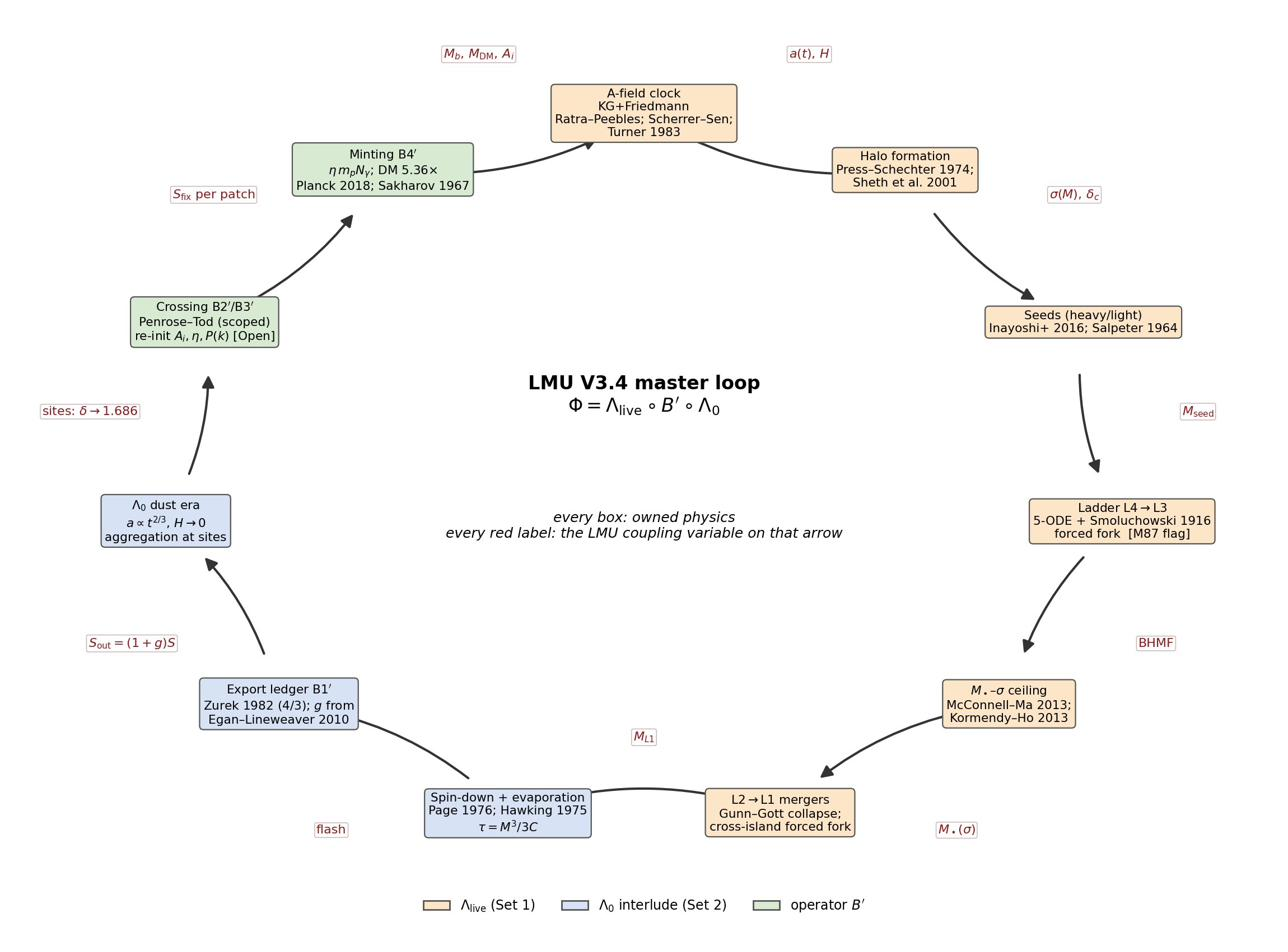
\includegraphics[width=0.99\textwidth]{fig1_wiring.png}
\caption{The master loop. Boxes are owned equations (colour = phase); red labels are the LMU coupling variables. The architecture --- the choice of arrows --- is the only LMU claim in this figure. \design}
\label{fig:wiring}
\end{figure}

\textbf{How the parts map onto the cycle.} Part~I is the live-phase matter sector ($\Lambda_{\rm live}$, the ladder L4$\to$L1); Part~II is the live-phase clock (the A-field) and its verification record; Part~III is the interlude $\Lambda_0$ (the corrected dust background) and the closure ledger; Part~IV is the transition operator $B'$ (export--partition); Part~V is the result of composing them ($\Phi$, the fixed band and the Tolman ledger); Part~VI is the verification and empirical confrontation archive; Part~VII the measured-input stress audit and the $V_{\min}$ Decision Record; Part~VIII the single open ledger; Part~IX the master attribution. \design

\section{The three-layer reading of the loop (V3.21 re-architecture)}
Every \emph{measured} quantity in this document is \emph{intra-aeon} --- observed through tiny sub-zones inside $L0$ --- so it is \emph{agnostic to how the reset works} and carries across unchanged. Only the reset/inter-aeon joint (the single unobserved step) is model-dependent. V3.21 makes that explicit by reading the loop in three layers; no measured fact moves, and the residual is unchanged --- this is an architectural reorganization, \emph{not} a physics verdict (V4.0 stays reserved for DESI-Y5, M87, or a solved rebirth).
\begin{center}\small
\begin{tabular}{@{}p{0.15\textwidth}p{0.79\textwidth}@{}}\toprule
\textbf{Layer A} & \emph{Intra-aeon physics} --- all measured \Fact{} (ladder Part~I; $A$-field/DESI Part~II; $L0$ ledger Part~III; results Part~V; verification Part~VI). Route-agnostic; identical under either joint below.\\
\textbf{Layer B} & \emph{The reset joint} --- the one part that is model-selectable. \textbf{B-primary} $=$ nucleation (SVT substrate $+$ Coleman--De Luccia bubble; Part~IV). \textbf{B-alt} $=$ Penrose conformal rescale, demoted but fully kept (the $V_{\min}$ trichotomy, G1/G2, $z_{\rm aeon}$; Part~VII).\\
\textbf{Layer C} & \emph{The shared residual} --- a $\Phi_{\rm gen}$ false-vacuum branch must exist/be accessible. Required by \emph{both} joints (nucleation tunnels from it; the rescale blueshifts to it), so posited once. It is the document's existing item~(D) (the in-aeon generator) seen from the energy side $=$ an inflaton-level posit $=$ the field's universal frontier (CC problem / Weinberg), not an LMU-specific defect.\\
\bottomrule
\end{tabular}
\end{center}
\textbf{Notation --- four distinct objects (do not conflate; two are $\sim$120 orders apart in energy density).} The overloading of ``$A$''/``$\Lambda$'' across these is the chief source of reasoning drift; they are kept separate throughout.
\begin{center}\small
\begin{tabular}{@{}p{0.13\textwidth}p{0.30\textwidth}p{0.12\textwidth}p{0.37\textwidth}@{}}\toprule
symbol & what it is & scale & role\\\midrule
$\Lambda_{\rm DE}$ (author types ``$A$'') & thawing quintessence, $V=\tfrac12 m^2A^2$, rolls to $0$ in $L0$ & $\sim10^{-3}$\,eV & late dark energy $\to$ DESI $w(z)$\\
$q$ & SVT/Volovik substrate variable & trans-Planckian & self-tunes $\Lambda\to0$ via $\Lambda=\epsilon(q)-\mu q$\\
$\Phi_{\rm gen}$ & per-aeon generator / plateau inflaton $=$ item~(D) & $\sim10^{16}$\,GeV & makes $P(k)$ \emph{and} its reheating is the bang's heat\\
$\Phi_{\rm gen}$ false vacuum & the metastable state $\Phi_{\rm gen}$ sits in before rolling & $\sim10^{16}$\,GeV & the bang's fuel (Layer~C)\\
\bottomrule
\end{tabular}
\end{center}
The ignition fuel is $\Phi_{\rm gen}$'s false vacuum ($\sim10^{16}$\,GeV), a \emph{different field} from the meV-scale dark energy $\Lambda_{\rm DE}$ --- it is \emph{not} ``$\Lambda_{\rm DE}$ cranked up.'' The document already proves the $A$-field cannot be the fuel (dead-end C1, Part~VIII: a false vacuum bolted onto $V$ gives a GUT-scale $\Lambda$ today, excluded), so the fuel must be the separate generator $\Phi_{\rm gen}$, which is item~(D). \Auditor

\clearpage

\part{The matter ladder --- L4 to L1 as a dynamical system}
\setcounter{section}{0}\setcounter{equation}{0}\setcounter{figure}{0}

% =====================================================================
\section{Overview --- what this module is, and how to read it}
The body of the framework (the main worldview document) argues in words that ordinary matter climbs a two-way ladder of black holes, L4$\to$L1, ranked by an object's \emph{position in the eating process} rather than by its mass. Module L turned that picture into \emph{equations of motion}. \textbf{This module does three things with those equations and then explains what the results mean:}
\begin{enumerate}[leftmargin=1.5em,itemsep=2pt]
\item \textbf{Integrates} the equations forward in cosmic time for four different environments, and asks whether one set of equations reproduces the four observed kinds of object (\S4, Fig.~1).
\item \textbf{Sweeps} the free coefficients to ask whether the structural results are real physics or artifacts of the particular numbers chosen (\S6, Fig.~2).
\item \textbf{Scales up} from one hole to a whole population, via the coagulation (Smoluchowski) equation, to ask what mass function the ladder predicts (\S7, Fig.~3).
\end{enumerate}

\textbf{How the model is used, in one sentence.} It is a \emph{forward map from environment to fate}: hand it the conditions a hole is born into --- the depth of its host ($\sigma$), how much gas it is fed ($f_{\rm Edd}$, $\dot M_{\rm cool}$), and how many companions it can eat ($n_{\rm gal}$) --- and it returns where that hole ends up: its final mass, its spin, the rung it occupies, and whether it is ejected or quenched on the way. One does not tell it the answer; one tells it the environment and reads off the outcome.

\textbf{What to keep in mind while reading (stated once, up front).} These equations are standard galaxy-evolution physics --- accretion, dynamical friction, spin evolution, feedback --- assembled in a particular way. \textbf{Nothing here distinguishes the framework from $\Lambda$CDM}, and the absolute masses are calibration, not predictions. What is genuine is \emph{structure}: which correlations fall out of the dynamics without being inserted, and whether they survive when the numbers are varied. The honest accounting is gathered in \S8. \Design\ (the assembly) / \Hyp\ (the physics).

% =====================================================================
\section{The equations of motion}
The state of one climbing system is Pitarn's four channels plus the running mass and a merger counter:
\begin{equation}
\Big[\ \underbrace{\Mbh}_{\text{mass}}\ ;\ \underbrace{a_\ast}_{\text{Spin}},\ \underbrace{M_g}_{\text{Gas}},\ \underbrace{n_{\rm gal}}_{\text{Near-Galaxy}},\ \underbrace{N}_{\text{merger count}}\ \Big],\qquad \text{environment fixed by }(\sigma,\ \rho_{\rm DM}).
\end{equation}
Two reductions from Module L are made explicit: the gas channel is carried as a reservoir mass $M_g$, and the dark-matter density enters through $\sigma$ (which sets both the escape speed and the dynamical-friction rate). Throughout, $q$ is a merger mass ratio and $\eta=q/(1+q)^2$.

\subsection{Growth --- accrete (Gas) plus eat (Near-Galaxy $\times$ DM)}
\begin{equation}
\boxed{\ \dot\Mbh=\dot\Mbh^{\rm acc}+\dot\Mbh^{\rm mrg}\ }
\end{equation}
\begin{equation}
\dot\Mbh^{\rm acc}=f_{\rm Edd}\;\underbrace{\frac{M_g}{M_g+M_{g,\frac12}}}_{\text{supply throttle}}\;\underbrace{\mathcal{C}(\Mbh,\sigma)}_{\text{feedback cap}}\;\frac{\Mbh}{\tau_{\rm Sal}}.
\label{eq:acc}
\end{equation}
\begin{equation}
\mathcal{C}(\Mbh,\sigma)=\begin{cases}1, & f_{\rm Edd}>1\ \ (\text{super-Eddington, photon-trapped})\\[2pt] \max\!\big(0,\,1-(\Mbh/\Msig)^{\beta}\big), & f_{\rm Edd}\le1\ \ (\text{King regulation})\end{cases}
\end{equation}
Cold dense gas feeds the hole at the Salpeter $e$-fold $\tau_{\rm Sal}\!\approx\!45$~Myr; a thinning reservoir starves it (the throttle is the smaller of the Bondi and Eddington rates). The cap $\mathcal C$ is the King (2003) self-regulation: \emph{sub-Eddington} growth shuts off as $\Mbh\!\to\!\Msig$ (McConnell--Ma 2013). \textbf{The one structural assumption} is the upper branch --- \emph{super-Eddington} accretion in a dense cocoon is radiatively trapped, so it evades the $\Msig$ wind and can overshoot (the only way an isolated hole becomes over-massive, \S5). \Fact\ (Bondi, Salpeter, King) / \Hyp\ (super-Edd evades feedback; Inayoshi, Haiman \& Ostriker 2016).
\begin{equation}
\dot\Mbh^{\rm mrg}=\Gamma_{\rm mrg}\,q_{\rm typ}\,\Mbh,\qquad
\Gamma_{\rm mrg}=K_{\rm mrg}\,n_{\rm gal}\,\Big(\frac{\sigma}{\sigma_0}\Big)^{-1}\ \ \big[\text{Chandrasekhar }\rho_{\rm DM}/\sigma^3\text{, folded}\big].
\label{eq:mrg}
\end{equation}
Eating needs a companion ($n_{\rm gal}$) and a sinking rate set by dynamical friction. \Fact\ (drag) / \Hyp\ (read as the L3$\to$L2 climb).

\subsection{Spin --- up by coherent Gas, down by Near-Galaxy mergers}
\begin{equation}
\boxed{\ \dot a_\ast=\underbrace{+\,C_{\rm acc}\,\frac{\dot\Mbh^{\rm acc}}{\Mbh}\,(a_{\rm eq}-a_\ast)}_{\text{coherent accretion spins up}}\ \underbrace{-\,C_{\rm mrg}\,\frac{\Gamma_{\rm mrg}}{1+N}\,a_\ast}_{\text{random mergers spin down}}\ }
\label{eq:spin}
\end{equation}
Prograde accretion drives $a_\ast\!\to\!a_{\rm eq}\!=\!0.998$ (Thorne 1974); many misaligned mergers random-walk it down as $a_\ast\!\approx\!a_0/\sqrt{1+N}$, whose differential form fixes $C_{\rm mrg}=\tfrac12$ (\emph{not} free; Hughes \& Blandford 2003). This is the \emph{merger-phase} spin-down that protects the survivor at the gate (\S5); it is distinct from the terminal Page spin-down at the very end.

\subsection{Gas, environment, and the two off-ramps}
\begin{equation}
\dot M_g=\dot M_{\rm cool}(t)-\dot\Mbh^{\rm acc},\qquad
\dot n_{\rm gal}=-\Gamma_{\rm mrg},\qquad \dot N=+\Gamma_{\rm mrg},
\label{eq:gasenv}
\end{equation}
with cooling inflow set by the halo and the companion supply $n_{\rm gal}\!\to\!0$ as the centre eats its surroundings --- which is what turns an L2 into the lone L1. The escape speed is the DM-set depth, $v_{\rm esc}=\xi\sigma$ ($\xi\!\simeq\!2$). The two ways off the climb:
\begin{align}
\text{\bf fall:}\quad & \text{eject}\iff v_{\rm recoil}(a_\ast,q,\theta)>v_{\rm esc}(\sigma),\quad v_{\rm recoil}=\sqrt{v_m^2+v_s^2},\\
&\qquad v_m=A_{\rm kick}\,\eta^2\tfrac{1-q}{1+q}\,(1+B_{\rm kick}\,\eta),\quad v_s=H_{\rm kick}\,\eta^2(a_2-q\,a_1)\cos\theta,\notag\\
\text{\bf die:}\quad & \text{quench}\iff M_g\to0\ \Rightarrow\ \dot\Mbh^{\rm acc}\to0\ \ (\text{starvation; Larson et al.\ 1980; Balogh et al.\ 2000}),
\end{align}
with $A_{\rm kick}=1.2\times10^4$, $B_{\rm kick}\approx-0.93$, $H_{\rm kick}=6.9\times10^3$ km\,s$^{-1}$ (Gonz\'alez 2007; Fitchett 1983; Campanelli 2007); the non-spinning recoil peaks at $\sim$175 km\,s$^{-1}$, superkicks of 2000--5000 km\,s$^{-1}$ need high in-plane spin. \Fact

% =====================================================================
\section{Coefficients: what is fixed by physics, what is calibrated}
\noindent\emph{Unit declarations (2026-06-12 audit).} $K_{\rm mrg}$ carries Gyr$^{-1}$ (previously unitless in the table; the unit lived only in the scripts). \textbf{Flag:} the demo script \texttt{forward\_map\_demo.py} implements $\Gamma_{\rm mrg}\propto(\sigma/\sigma_0)^{+1}$ with $K=0.08$~Gyr$^{-1}$ --- the \emph{opposite} $\sigma$-power to eq.~\eqref{eq:mrg}; the two laws coincide only at $\sigma\simeq474$~km\,s$^{-1}$. Eq.~\eqref{eq:mrg} (Chandrasekhar-paced, decreasing in $\sigma$) is authoritative; a demo rerun on the corrected law is queued, and until then the four-galaxy classification figures carry this flag. The Smoluchowski kernel normalization likewise carries [Gyr$^{-1}$ per unit comoving number density]; units previously lived only in code. \Auditor

\begin{center}\small
\begin{tabular}{@{}lll@{}}
\toprule
\textbf{Physics-fixed (not free)} & \textbf{Calibrated-free (5)} & \textbf{Per-archetype inputs} \\
\midrule
$\tau_{\rm Sal}=45$ Myr & $C_{\rm acc}=1.5$ (spin-up rate) & $\sigma$ (host depth) \\
$a_{\rm eq}=0.998$ (Thorne) & $K_{\rm mrg}=0.45$~Gyr$^{-1}$ (merger norm.; $\sigma_0=200$~km\,s$^{-1}$) & $f_{\rm Edd}(t)$ (Eddington ratio) \\
$C_{\rm mrg}=\tfrac12$ (from $a\!\propto\!N^{-1/2}$) & $\beta=2$ (feedback sharpness) & $\dot M_{\rm cool}(t)$ (gas supply) \\
$\xi=2$ ($v_{\rm esc}=\xi\sigma$) & $M_{g,\frac12}=10^{7}\,\msun$ & $M_g(0)$ (initial reservoir) \\
$A,H$ recoil; $\Msig$ (McConnell--Ma) & $q_{\rm typ}=0.25$ & $n_{\rm gal}(0)$ (companions) \\
\bottomrule
\end{tabular}
\end{center}
\textbf{The decisive choice:} $\sigma$ and $n_{\rm gal}$ are set \emph{independently} --- a hole can sit in a deep well ($\sigma=300$) with \emph{zero} companions (the relic). Tying environment to mass was a logged error; keeping them independent is exactly what lets the ranking be by eating-position, not size. \Design

\medskip\noindent\textbf{Provenance audit (document-wide, R6/R7 --- four classes, not two).} The table above is the ladder-dynamics scope; read across the whole document every number falls in one of four classes, and the line that matters is \emph{input declared as input} (legitimate --- exactly as $\alpha$ or the quark masses are inputs in the Standard Model) versus \emph{fitted then claimed as a prediction} (the only failing kind). Full census:
\begin{center}\footnotesize
\begin{tabular}{@{}p{0.235\textwidth}p{0.235\textwidth}p{0.235\textwidth}p{0.235\textwidth}@{}}
\toprule
\textbf{(1) Derived / physics-fixed} & \textbf{(2) Calibrated-free, \emph{disclaimed}} & \textbf{(3) Declared input (by design)} & \textbf{(4) Fitted-and-claimed (the failing kind)} \\
\midrule
$\tau_{\rm Sal}$, $a_{\rm eq}$, $C_{\rm mrg}\!=\!\tfrac12$, $\xi$, $A/H$ recoil, $\Msig$; and the R6 set --- $M_{\rm Nariai}\!=\!\sqrt{27}/2$, Zurek $4/3$, pair-$T$, $S_{\rm BH}$, $\tau_{\rm evap}$, $\Omega_c/\Omega_b$, the mint chain (13/13 reproduced from constants) &
$C_{\rm acc}$, $K_{\rm mrg}$, $\beta\!=\!2$ (feedback sharpness), $M_{g,1/2}$, $q_{\rm typ}$; per-archetype $f_{\rm Edd}(t)$, $\dot M_{\rm cool}(t)$, $M_g(0)$, $n_{\rm gal}(0)$; the absolute masses &
$A_i\!=\!2.70\,M_p$, $\eta$, $P(k)$ targets ($n_s,A_s,r,f_{\rm NL}$), the $V_{\min}$ sign, $\Omega_k$, $z_{\rm aeon}$ --- the B3$'$ re-initialization data &
\emph{empty} --- no value is fitted then claimed as a prediction. The one historical slip, $\beta\!\approx\!0.7$, was an \textbf{R9 attribution} error (right number, wrong relation --- see note), \emph{not} a fit. Watch (flagged, not claimed): $f_{\rm coh}\!\gtrsim\!0.15$ (item J3); the $K_{\rm mrg}$ demo $\sigma$-power (above) \\
\bottomrule
\end{tabular}
\end{center}
\noindent\textbf{Reading it.} Class~(2) is named as calibration, not prediction: the document states that matching the four anchors is ``a consistency demonstration, not a fit-test,'' that the absolute masses ``remain calibration,'' and (table footnote, \S\,Computation~1) that the isolated-mass archetype \emph{overshoots} the corrected NGC~1277 anchor by $\sim$0.6\,dex --- calibration named as such, with its own overshoot disclosed. Class~(3) is the same epistemic status as $\alpha$ in the Standard Model: measured or posited, derived by no one, ``said out loud'' (B3$'$) --- not a hidden fit. Class~(4) --- a value tuned then claimed as a prediction --- is \emph{empty}. The one error usually filed here is a \emph{different} failure mode: $\beta\!\approx\!0.7$ was a \emph{correctly-computed} slope (it matches the published stellar $M_{*}$--$M_{500}$ slope of Kravtsov et al.\ 2018) that was \emph{mis-attributed} to the black-hole $M_\bullet$--$M_{\rm halo}$ relation, whose owned slopes are all $\ge1$ --- an R9 identity slip, not a fit; caught at item~(E). Because the superseded result ($0.14$\,dex/decade) is numerically coincident with the lower edge of the corrected owned-slope band ($0.15$--$0.27$), the headline survived: the arithmetic was sound, only the relation label was wrong. No number in the framework is presented as a prediction while secretly fitted; that property, not the absence of inputs, is what keeps the work on the science side of the line. \Auditor\ \emph{Input-count note (V3.16):} within class~(3) the $A$-field sector carries both $A_i$ and (implicitly) $w_0$, but they are \emph{not independent} --- fixing the potential and the measured $\Omega_{\rm DE0}=0.69$ determines $A_i$ by shooting (Part~II Run~2), so the live $A$-sector has effectively \emph{one} free parameter, the mass $m$. The slow-roll heuristic makes the link explicit: $\epsilon=2(M_p/A_i)^2$ with $A_i=2.70\,M_p$ gives $\epsilon\approx0.27$ and $w_0\approx-1+\tfrac23\epsilon\approx-0.82$ (the full integration's $-0.91$; slow-roll is loose at this $\epsilon$). A bookkeeping tightening by one, not new physics.


% =====================================================================
\section{Computation 1 --- four environments, four fates}
The same equations \eqref{eq:acc}--\eqref{eq:gasenv} are integrated from a $10^4\,\msun$ seed to 13.5 Gyr with four input sets (field, cluster, isolated-massive, dwarf).

\begin{figure}[h]
\centering
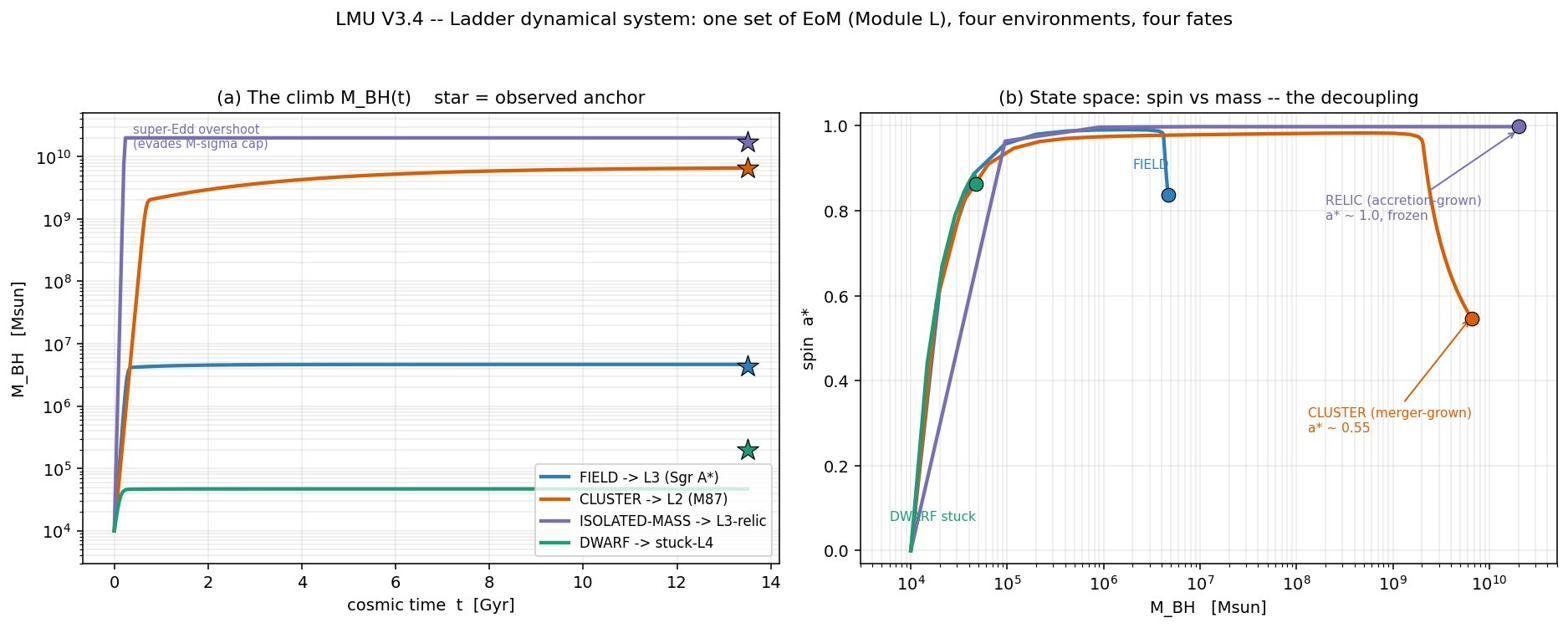
\includegraphics[width=\textwidth]{ladder_dynamics.png}
\caption{\textbf{(a)} The climb $\Mbh(t)$: one set of equations, four environments, four fates; stars are observed anchors (Sgr A*, M87, NGC 1277, dwarf IMBHs; the NGC~1277 star is drawn at the superseded 2012 anchor --- the corrected Walsh 2016 mass is $4.9\times10^{9}\,\msun$, see table footnote). \textbf{(b)} State space $a_\ast$ vs $\Mbh$: at fixed $\sigma=300$ the cluster (merger-grown) lands at $a_\ast\!\approx\!0.55$ while the relic (accretion-grown) freezes at $a_\ast\!\approx\!1.0$.}
\end{figure}

\begin{center}\small
\begin{tabular}{@{}lcccccl@{}}
\toprule
archetype & $\Mbh$ (model) & anchor & $a_\ast$ & dex/$\Msig$ (obs) & $N_{\rm mrg}$ & $f_{\rm eject}$ \\
\midrule
FIELD $\to$ L3 (Sgr A*) & $4.6\times10^6$ & $4.3\times10^6$ & 0.84 & $+0.05$ ($+0.01$) & 0.6 & 41\% \\
CLUSTER $\to$ L2 (M87) & $6.6\times10^9$ & $6.5\times10^9$ & 0.55 & $+0.50$ ($+0.50$) & 5.9 & 0\% \\
ISOLATED-MASS $\to$ relic & $2.0\times10^{10}$ & $4.9\times10^{9}$\,$^{\dagger}$ & 1.00 & $+0.99$ ($+0.24$)$^{\dagger}$ & 0.0 & 0\% \\
DWARF $\to$ stuck-L4 & $4.7\times10^4$ & $\sim2\times10^5$ & 0.86 & $+0.01$ & 0.1 & 83\% \\
\bottomrule
\end{tabular}
\end{center}
{\footnotesize $^{\dagger}$\,Anchor updated (V3.5): the NGC~1277 anchor is the Walsh et al.\ (2016) adaptive-optics dynamical mass $(4.9\pm1.6)\times10^{9}\,\msun$ (confirmed by Krajnovi\'c et al.\ 2018), superseding the van den Bosch et al.\ (2012) value in use when this run was calibrated (now retired; Part~V \S4). The archetype's $2.0\times10^{10}$ output therefore \emph{overshoots} the corrected anchor by $\sim$0.6~dex, and NGC~1277 is \emph{lighter} than M87 --- the relic claim rides the $n=6$ sample offset $+0.22\pm0.09$~dex (Part~VI), not this single anchor; the extreme-overmass flagship is TON~618. The parenthesised observed offset ($+0.24$~dex) is the corrected anchor's M--$\sigma$ residual at the adopted $\sigma=317$~km\,s$^{-1}$ (Part~VI \S5). \Auditor}


\textbf{What it means.} The four rungs of the ladder are not four separate stories that each need their own explanation; they are \emph{one mechanism} --- the same five equations --- run from four starting environments. A field galaxy fed a steady trickle of gas regulates itself onto the $\Msig$ relation and stops (L3). Put the same seed in a company-rich cluster and mergers carry it past $\Msig$ into a cluster-dominant hole (L2). Give it a dense early gas cocoon but no companions and it overshoots by super-Eddington accretion, then freezes --- an over-massive but un-climbed relic (L3-relic). Starve it in a shallow dwarf and it stalls near its seed (stuck-L4). The model's job is done when the \emph{environment alone} selects the fate; that it lands on the four real anchors is the consistency check that the assembled physics is at least self-consistent.

% =====================================================================
\section{What emerges --- structural results, not tuned}
The spin coefficients are the \emph{same} for all four runs; the following were not fitted per object.
\begin{itemize}[leftmargin=1.3em,itemsep=3pt]
\item \textbf{Spin remembers how the hole grew.} At fixed $\sigma=300$, cluster and relic differ by $\Delta a_\ast=+0.45$ purely because one grew by mergers (spun down) and the other by accretion (spun up). Spin is therefore a \emph{fossil of assembly history} that is independent of mass --- the framework's one genuinely non-circular structural expectation (its carry-through/C5 signature). \Hyp
\item \textbf{The survivor cannot be thrown out.} The cluster candidate ($a_\ast=0.55$, $v_{\rm esc}=600$ km/s) has $f_{\rm eject}=0\%$ --- protected on \emph{both} coordinates at once, spun down and deep-welled --- while the spun-up shallow-welled bottom has $f_{\rm eject}=41$--$83\%$ per merger. Ejection recycles only the light bottom, never the winner. This supplies the mechanism the survivor argument otherwise only asserts. \Hyp
\item \textbf{Over-massiveness is forced, not chosen.} An isolated hole ($n_{\rm gal}=0$) has $\dot\Mbh^{\rm mrg}=0$, so it \emph{cannot} be built over-massive by eating; the only route left is super-Eddington accretion. The relic's $+0.99$ dex offset is thus forced to be an accretion-overshoot signature --- which makes it a testable prediction (\S9), not a fudge. \Hyp
\end{itemize}

% =====================================================================
\section{Computation 2 --- are the structural results real? (robustness)}
A worry about \S5 is that those three results might be artifacts of the particular coefficients chosen. To test this, all five free coefficients were varied together over factor-2--3 ranges (Monte Carlo, $N=400$, stiff Radau integrator), re-running cluster, relic, and field for each set.

\begin{figure}[h]
\centering
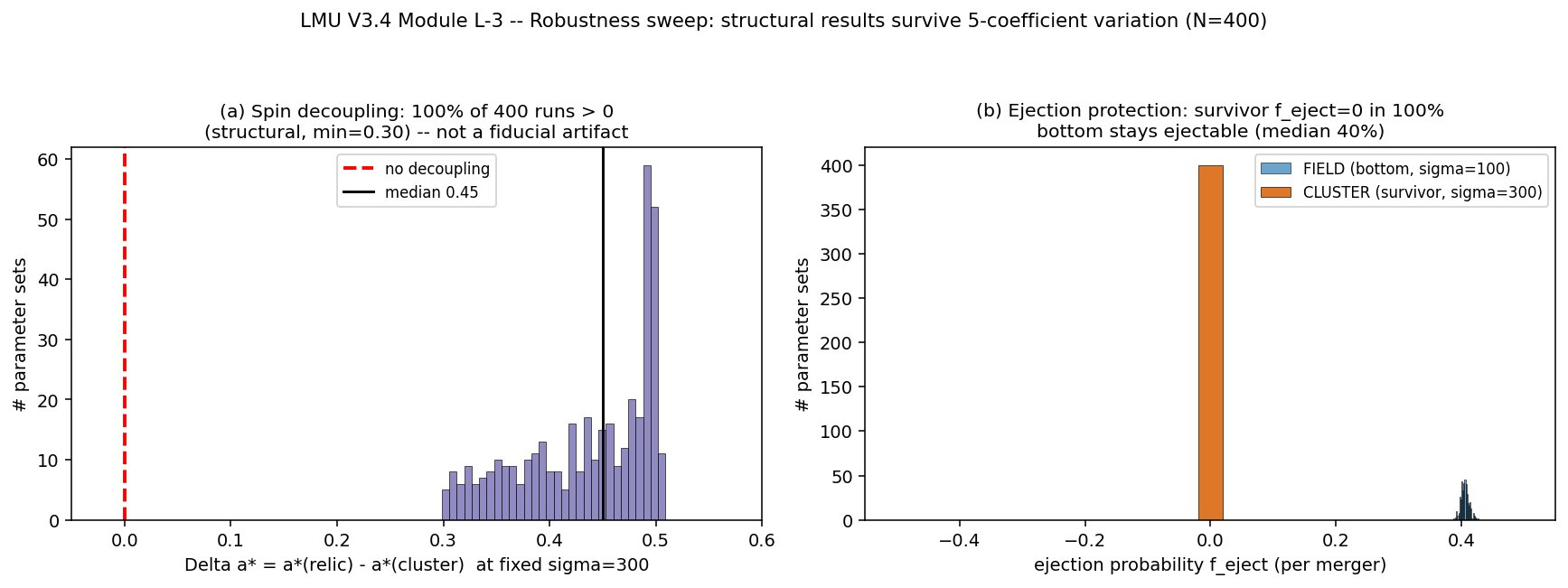
\includegraphics[width=\textwidth]{ladder_robustness.png}
\caption{\textbf{(a)} The spin decoupling $\Delta a_\ast$ across 400 random coefficient sets: it is positive in 100\% of them (median 0.45, minimum 0.30), never vanishing. \textbf{(b)} Ejection probability: the cluster survivor stays at $f_{\rm eject}=0\%$ in 100\% of the space, while the field bottom remains ejectable (median 40\%).}
\end{figure}

\textbf{What it means.} The decoupling and the protection are not tuned coincidences --- they survive the entire free-parameter space, because they are forced by the \emph{topology} of the two situations, not by the numbers. An isolated hole has no companions, hence no spin-down term in Eq.~\eqref{eq:spin}, so it must reach $a_\ast\!\to\!a_{\rm eq}$; a merger-rich hole always carries the spin-down term, so it must end lower. The \emph{sign} of $\Delta a_\ast$ is therefore guaranteed; only its \emph{size} (how far the cluster spins down) depends on the coefficients, and that stays observably large (median 0.45). Likewise the survivor sits in a deep well and is spun down, so its recoil never reaches escape, whatever the coefficients. In short: \S5's structural claims are promoted from ``happens at the fiducial point'' to ``happens generically.'' The absolute masses, by contrast, do move with the coefficients --- they remain calibration.

% =====================================================================
\section{Computation 3 --- from one hole to a population}
A single trajectory describes one hole. The whole ladder is a \emph{population}, governed by the coagulation (Smoluchowski 1916) equation that Module L opened,
\begin{equation}
\begin{aligned}
\partial_t\,n(M,t)=\ &\underbrace{\tfrac12\!\int_0^M\! K\,n(M')\,n(M{-}M')\,dM'\ -\ n(M)\!\int_0^\infty\! K\,n(M')\,dM'}_{\text{mergers (climb-by-eating)}}\\[2pt]
&-\ \underbrace{\partial_M\!\big[\dot M_{\rm acc}(M)\,n\big]}_{\text{gas climb}}\ -\ \underbrace{\Gamma_{\rm ej}(M)\,n}_{\text{recoil sink}}\ +\ \underbrace{S(M,t)}_{\text{seeds}},
\end{aligned}
\end{equation}
with the friction-motivated kernel $K\!\propto\!(M_i{+}M_j)$, gas advection up to the $\Msig$ ceiling, the recoil sink acting only on low-mass merger products (the \S5 survivor-protection result, applied at the population level), and a declining seed source. The scheme conserves mass to $0.1\%$ (a coagulation-solver check), and the recoil branching, not a continuous decay, is what makes it physical.

\begin{figure}[h]
\centering
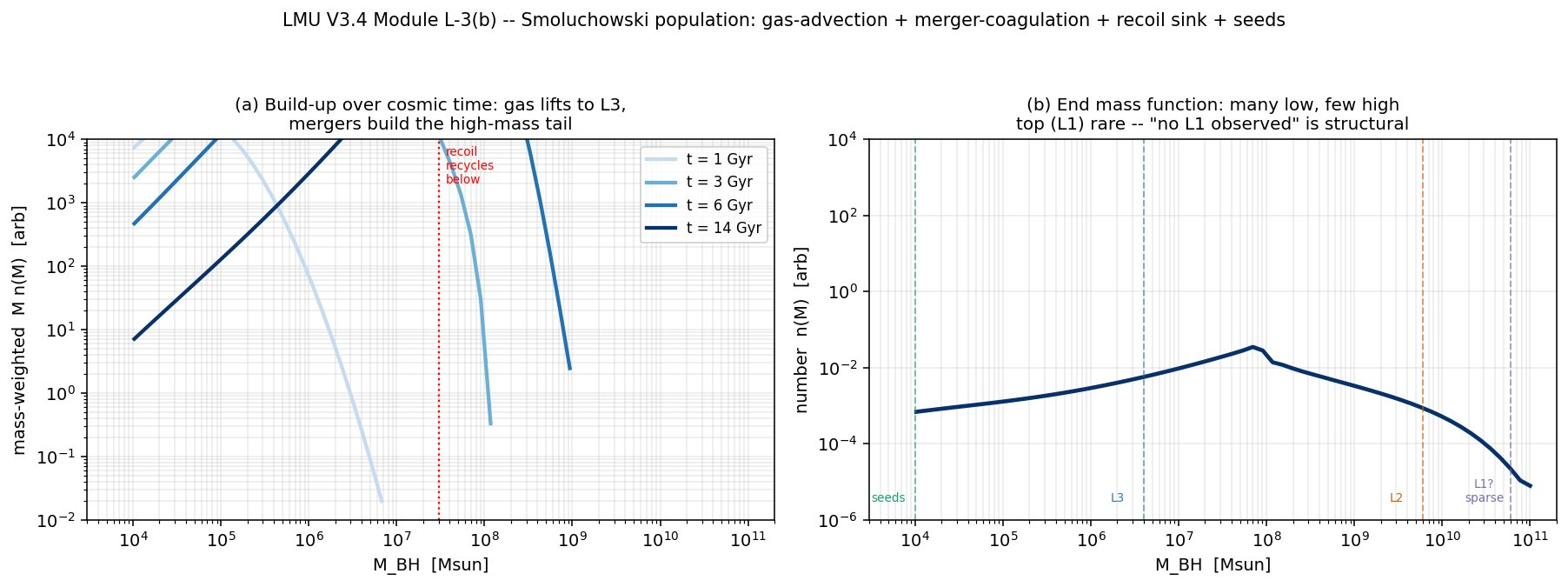
\includegraphics[width=\textwidth]{ladder_population.png}
\caption{\textbf{(a)} Build-up of the black-hole mass function over cosmic time: gas accretion lifts seeds to the L3 scale, mergers build the high-mass tail, recoil recycles the bottom. \textbf{(b)} The end-state mass function is steeply declining --- many low-mass holes, very few high-mass ones --- so the very top of the ladder is reached by almost nothing.}
\end{figure}

\textbf{What it means.} Read as a population, the ladder predicts exactly the shape one sees: a black-hole mass function dominated by ordinary galaxy-centre (L3) holes, falling steeply toward the cluster-dominant (L2) scale, with the survivor (L1) end essentially empty. \textbf{The rarity of the top is structural} --- it is the natural outcome of a cascade in which most objects settle or are recycled long before reaching the summit. This is the population-level reason the main text gives for why L1 has no observed example: not a gap in the data, but a consequence of the dynamics. The recoil sink shows its hand at the bottom, where low-mass spun-up merger products are kicked out and recycled rather than retained.

\subsection{Refinement --- the high-mass abundance from first principles}
The single-population run fixes the mass-function \emph{shape} but calibrates the merger efficiency, so the \emph{number} of L2-scale holes is not yet first-principles. The fix is to resolve the population by environment: most holes live in shallow field hosts (low $\sigma$, few companions $\to$ L3 on $M$--$\sigma$), a minority in deep cluster hosts (high $\sigma$, many companions $\to$ L2), and these environments occur with the abundance set by the observed velocity-dispersion function (VDF; Sheth et al.\ 2003). Running the dynamics across a $\sigma$ grid and weighting by the VDF gives the black-hole mass function as a convolution, $\mathrm{BHMF}=\mathrm{VDF}\circ M_\bullet(\sigma)$.

\begin{figure}[h]
\centering
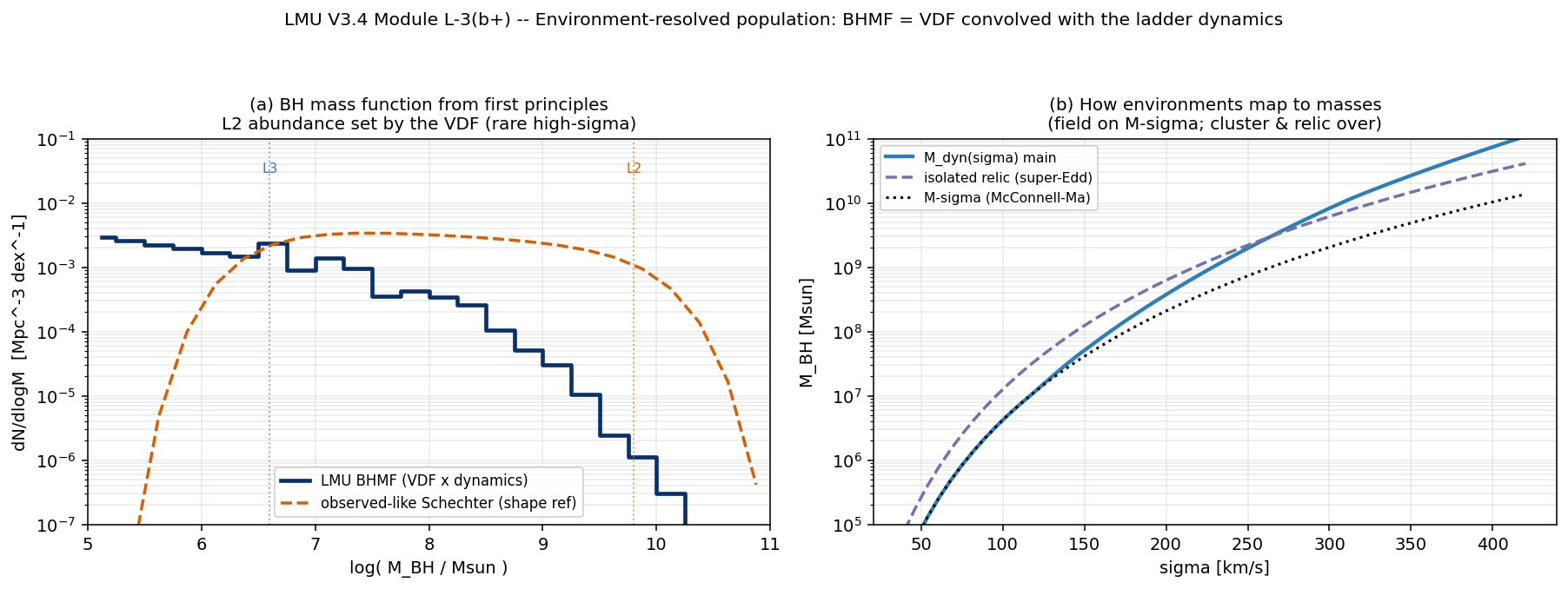
\includegraphics[width=\textwidth]{ladder_bhmf.png}
\caption{\textbf{(a)} The BH mass function from the environment-weighted dynamics: declining and observed-like, with the L2 end rare \emph{because deep hosts are rare} ($n_{\rm L3}/n_{\rm L2}\!\sim\!\mathcal{O}(10^2)$ --- VDF-parameter and $\sigma$-bin sensitive (ranging ${\sim}20$--$500$ across reasonable choices), with the top-sparsity following from the dispersion function rather than a tuned merger rate). \textbf{(b)} How environments map to masses: the dynamics produces $M$--$\sigma$ at low $\sigma$ (field) and rises above it with merger spin-down at high $\sigma$ (cluster), plus the over-massive isolated-relic branch.}
\end{figure}

\textbf{What it means.} The L2 abundance is now first-principles \emph{given the VDF}: the top of the ladder is rare because the deep environments that build it are rare, the rarity following from the dispersion function (deep hosts are rare) rather than from a tuned merger rate --- though the exact ratio is VDF/bin-dependent and not a sharp prediction. This remains the standard $\mathrm{BHMF}=\mathrm{VDF}\times M$--$\sigma$ construction --- non-discriminating --- the framework's additions being the over-massive relic branch and the spin structure; the VDF parameters and the environment model are approximate, and the low-mass (dwarf-IMBH) end is over-produced (observationally uncertain anyway). \Hyp

% =====================================================================
\section{What this model is for --- and what it cannot do}
\textbf{What it is for.} (i) A \emph{translator}: it converts the verbal ladder into a quantitative forward map, so the picture can be checked for internal consistency rather than only asserted. (ii) A \emph{fingerprinting tool}: because spin records assembly history (\S5), the model says that a direct spin measurement reads off whether a hole was merger-built or accretion-built --- a use with a concrete observational target (\S9). (iii) A \emph{population predictor of shape}: it says the mass function must be top-sparse, which is why no L1 is seen.

\textbf{What it cannot do (and does not claim).}
\begin{itemize}[leftmargin=1.3em,itemsep=2pt]
\item \textbf{It does not beat $\Lambda$CDM.} Every equation is standard galaxy-evolution physics; the model is a consistency statement of the framework's \emph{organising idea} (eating-position ranking, survivor, recycling), not a new prediction that discriminates between cosmologies.
\item \textbf{It does not predict absolute masses.} Five free coefficients plus per-archetype inputs mean matching four anchors is a consistency demonstration, not a fit-test. The weight is on the un-tuned structure of \S5--6, which survives the sweep.
\item \textbf{The $\Msig$ landing of the field is circular} --- the King mechanism is built to yield $\Msig$, so that is calibration, not a prediction. \Open
\item \textbf{The population's high-mass \emph{abundance} is not yet first-principles.} The single-population run gets the mass-function \emph{shape} (declining, top-sparse) but the \emph{number} of L2-scale holes needs the spread of environments ($\sigma$, $n_{\rm gal}$ distributions) folded in --- the next refinement. That pure light-seed mergers struggle to reach the top is itself the seeding bottleneck the main text acknowledges, resolved there by accretion and carry-through seeds.
\end{itemize}

% =====================================================================
\section{Falsifiers}
\noindent\textbf{Mandatory flag (V3.5; travels with every reuse of the ladder):} the cluster spin-down expectation ($a_\star\sim0.55$) is in tension with the M87 spin $a_\star\gtrsim0.8$ reported from EHT Doppler beaming (Drew et al.\ 2025, ApJL 984 L31, a lower limit; contested by Wong et al.\ 2025 polarimetry) --- status \open\ (contested), not falsified; the relic-side spin decoupling is unmeasurable in principle (Part~VI \S21). \textbf{V3.7 inversion:} the spin walk $a=a_0/\sqrt{1+N}$ (Hughes \& Blandford 2003) turns $a_\star\ge0.8$ into $N_{\rm misaligned}\le0.56$--$2.26$ (lower: pure walk from $a_0=0.998$; upper: walk allowing accretion re-spin, lift $\times1.45$) against the modeled $5.9$ --- tension factor $2.6$--$10.6$, i.e.\ an aligned-merger fraction $\ge62\%$ where the model assumed isotropy.
\begin{itemize}[leftmargin=1.3em,itemsep=2pt]
\item \textbf{Relic spin.} The model forces isolated over-massive relics (NGC 1277, Mrk 1216) to spin \emph{high} (accretion-frozen) while merger-built cluster BCGs spin \emph{low}. A local relic measured to spin low would break the decoupling. Testable by X-ray reflection (accreting relics) and, for the carry-through version, NewAthena $+$ LISA (late 2030s).
\item \textbf{A clear major merger in a relic} would break the ``grew fast, never climbed'' reading.
\item \textbf{Super-Eddington regulation.} If dense-cocoon super-Eddington accretion is shown to drive the same $\Msig$ wind as sub-Eddington, the isolated-relic over-mass mechanism (\S5) fails.
\end{itemize}

% =====================================================================
\section{Attribution --- the matter ladder}
\begin{center}\small
\begin{tabular}{@{}p{0.45\textwidth}p{0.49\textwidth}@{}}
\toprule
Element & Owner / source \\
\midrule
Four state variables; eating-position ranking; assembly & Pitarn (\Design) \\
Accretion: Bondi rate; Eddington/Salpeter $e$-fold & Bondi (1952); Salpeter (1964) \\
Super-Eddington in dense cocoon (evades feedback) & Inayoshi, Haiman \& Ostriker (2016) \\
Mergers: dynamical-friction sinking & Chandrasekhar (1943); White \& Rees (1978) \\
Spin-up to $a_{\rm eq}=0.998$ / merger spin-down $a\!\propto\!N^{-1/2}$ & Thorne (1974); Hughes \& Blandford (2003); Berti \& Volonteri (2008) \\
AGN feedback / $\Msig$ self-regulation; $\Msig$ normalisation & Silk \& Rees (1998); King (2003); McConnell \& Ma (2013) \\
Escape speed; recoil / superkick & NFW (1996); Gonz\'alez (2007); Campanelli (2007) \\
Starvation quenching & Larson et al.\ (1980); Balogh et al.\ (2000) \\
Population / coagulation equation & Smoluchowski (1916); Press \& Schechter (1974) \\
Integration, sweep, population solver, honest-status audit & editor pass (\Auditor) \\
\bottomrule
\end{tabular}
\end{center}

\vspace{4pt}\hrule\vspace{4pt}
{\small Module L-3 (consolidated) integrates, stress-tests, and scales up the equations of motion of Module L. It is a worldview's math pass, not a peer-reviewed result: every coefficient is classified, the calibration is named, the one load-bearing hypothesis (super-Eddington evades feedback) is flagged, and the structural results (spin decoupling, survivor protection, top-sparse mass function) are shown to survive a full free-parameter sweep. The ladder is the best-anchored part of the framework; this module makes its dynamics explicit, its results interpretable, and its freedoms visible.}

\clearpage

\clearpage

% ===================== PART II =====================
\part{The dark-energy field $A$ --- verification record, runs, and the DESI confrontation}
\setcounter{section}{0}\setcounter{equation}{0}\setcounter{figure}{0}

\begin{center}\fbox{\parbox{0.94\textwidth}{\small
\textbf{What this part verifies.} Sections 1--7 are the integrated verification record (formerly the separate companion document \emph{Verification of the LMU Dark-Energy Field A}, June 2026; carried here in full --- units $M_{\rm pl}=1$, $H_0=1$, $\Omega_{m0}=0.31$, $\Omega_{\rm DE0}=0.69$). They verify, by direct numerical integration, the dark-energy equation of state $w(a)$ of the scalar field $A$ --- the pair $(w_0,w_a)$ --- and test it against the value measured by DESI; they also establish the condition $V_{\min}=0\Rightarrow H\to0\Rightarrow$ asymptotic Minkowski that defines the Fork-Y endgame, and cross-validate the integration engine against published thawing-quintessence work. \textbf{Headline:} canonical thawing gives $w\ge-1$ always; it cannot reach the DESI central $(w_0,w_a)=(-0.84,-0.62)$, which requires past phantom crossing --- but it is \emph{not excluded}: the V3.8 chain pull pins the joint locus distance at $2.69\sigma$ (chain-Gaussian, $\rho=-0.894$) and $2.40\sigma$ (posterior-mass; $\Lambda$CDM itself sits at $2.83\sigma$ in the same convention --- DESI's quoted $2.8\sigma$; marginal $w_0$ within $1.3\sigma$). \textbf{What this does not establish:} a derivation of $V_{\min}=0$ (the Weinberg wall, \Open), or the $L0$-reservoir / entropy-dilution structure (an LMU interpretive layer, \Hyp). Section~8 adds this session's independent Run~2 ($A_i$ fixed, $m$ shot); \S9--13 carry the archived module's own PNGB cross-audit, honest status, and attribution.}}\end{center}

% ---------------------------------------------------------------------
\subsection*{The $A$-field in one paragraph --- what it must do, and what it cannot (V3.15)}
\noindent\textbf{What the field must do (the loop's demand, before any datum is fit).} The loop fixes the \emph{shape} of $A$'s history independently of the data: a zone must both accelerate now (the one observed fact) and later switch off ($A\to0$, $V\to0$) so it can relax into the $L0$ reservoir and the cycle can close. A bare cosmological constant cannot do the second --- a true $\Lambda$ is eternal de Sitter, reaching neither the Minkowski ($V_{\min}=0$) nor the AdS ($V_{\min}<0$) closure --- so the dark energy \emph{must} roll, and a field Hubble-frozen at high $z$ that only now releases is, by definition, \emph{thawing}. This is forced by the switch-off endgame, not chosen to fit DESI. The recombination --- the thawing taxonomy (Caldwell--Linder 2005; Scherrer--Sen 2008) $\times$ the cyclic switch-off requirement $\times$ the per-zone uniform-$A$ choice --- is the LMU linkage; the field equation itself (Klein--Gordon on an FRW background; Ratra--Peebles 1988; Wetterich 1988), the $w\ge-1$ bound (Vikman 2005), and the oscillate-to-dust endgame (Turner 1983) are borrowed, owned, and printed at the margin. The author's part is the wiring and the reading, not the equations. \Hyp\ / \Auditor

\noindent\textbf{The life of the field, in five stages.} \emph{(1) Frozen.} After the hot start $H$ is large and Hubble friction ($3H\dot A$ in Klein--Gordon) pins the field at $A_i\approx2.70\,M_p$; it sits at $w\approx-1$, an effective $\Lambda$, not yet rolling. \emph{(2) Thaw.} As the zone expands, matter dilutes ($\rho_m\propto a^{-3}$) and $H$ falls; once $H<m$ the friction releases and the field rolls down its potential, $w$ climbing off $-1$ --- the thawing onset (Scherrer--Sen 2008). \emph{(3) Today.} The field is mid-roll, $w_0\approx-0.91$, accelerating, near the crest of a transient acceleration ``mountain'' --- not $\Lambda$CDM's plateau. \emph{(4) Crest and descent.} $w$ rises through $-1/3$ and the acceleration ends (near $a\approx5.5$ for the pinned $m\approx0.80$ field; $a\approx2.9$ is the $m{=}1.0$ fiducial), the zone beginning to decelerate --- the published thawing signature (de Souza, Rodrigues \& Alcaniz 2025). \emph{(5) Switch-off.} The field reaches its minimum $V_{\min}=0$ at $A=0$, oscillates through it with $\langle w\rangle\to0$ (matter-like; Turner 1983), $\rho\to0$ and $H\to0$ --- asymptotic Minkowski, the reservoir state the loop requires. The engine is never an external supply: it is the potential energy stored in the field at $A_i$, released as $H$ falls. Matter is the \emph{brake} (it decelerates expansion), the field is the \emph{accelerant}, and acceleration ends when the field reaches its floor --- not when matter ``runs out.''

\noindent\textbf{What it cannot do, stated honestly (the DESI confrontation).} A single canonical scalar obeys $w=(K-V)/(K+V)\ge-1$ identically (Vikman 2005), so it cannot trace the DESI CPL central $(w_0,w_a)=(-0.84,-0.62)$, which dips into the past-phantom region $w<-1$. This is a miss of the \emph{central}, not an exclusion: the crossing is a property of the CPL straight-line ansatz, and fitting physical (non-CPL) thawing models to the same data is competitive --- so the crossing is most likely a \emph{parametrization artefact} (Dinda \& Maartens 2025, MNRAS 542 L31; de Souza et al.\ 2025), \emph{not} a measurement that the field is phantom. On the released DR2 chains the thawing locus is \emph{less disfavoured than $\Lambda$CDM itself} (Pantheon$+$: $2.69\sigma$/$2.40\sigma$ vs $\Lambda$CDM's $3.04\sigma$/$2.83\sigma$), and non-phantom is compatible at $\sim2\sigma$ --- so the honest status is \emph{disfavoured at the CPL central but not excluded}. The verdict reduces to one sharp test: does the phantom crossing survive a physical, non-CPL re-analysis with systematics resolved? Pre-registered falsifier (Fork Y, fixed): DESI-Y5 ($\sim$2027) sustaining $w(z)<-1$ at $\gtrsim3\sigma$ falls the canonical $A$; a quintom/$k$-essence upgrade would survive at the cost of a ghost and the lost ghost-free economy (ledger J2). Pinned values (R6, none inherited): $m\approx0.80\,H_0\approx1.2\times10^{-33}$\,eV, $A_i\approx2.70\,M_p$, $V(A)=\tfrac12 m^2A^2$ (floor at $A=0$), $w_0\approx-0.91$, $w_a\approx-0.15$, acceleration window $a\in(0.61,5.5)$. Full derivations, runs, figures, and attribution follow in \S\S1--13. \Open\ (the $V_{\min}$ sign and the Y5 verdict) / \Auditor

% ---------------------------------------------------------------------
\section{Equations --- the three-party balance}
A canonical scalar minimally coupled to gravity, homogeneous, in a flat FRW background:
\begin{align}
\text{field (Klein--Gordon):}\quad & \ddot A+3H\dot A+\frac{dV}{dA}=0,\qquad V(A)=\tfrac12 m^2A^2 \label{eq:p2kg}\\
\text{energy bookkeeping:}\quad & \frac{d}{dt}\Bigl(\underbrace{\tfrac12\dot A^2}_{K}+V\Bigr)=-3H\dot A^2 \label{eq:p2energy}\\
\text{equation of state:}\quad & \rho_A=\tfrac12\dot A^2+V,\quad p_A=\tfrac12\dot A^2-V,\quad
w_A=\frac{\tfrac12\dot A^2-V}{\tfrac12\dot A^2+V} \label{eq:p2eos}\\
\text{Friedmann:}\quad & 3H^2=\frac{\rho_{m0}}{a^3}+\rho_A,\qquad \rho_{m0}=3\,\Omega_{m0}=0.93 \label{eq:p2fried}\\
\text{DESI fitting form (CPL):}\quad & w(a)=w_0+w_a(1-a) \label{eq:p2cpl}
\end{align}
The three ``parties'' of the field equation are inertia $\ddot A$, Hubble friction $3H\dot A$ (the dissipative sink), and the restoring force $dV/dA$. All equations are standard \Fact\ (Klein--Gordon--FRW; thawing class: Scherrer \& Sen 2008; CPL: Chevallier--Polarski 2001, Linder 2003).

% ---------------------------------------------------------------------
\section{Result 1 --- $w(a)$ versus DESI (the $m$-scan)}
For each field mass $m$, the initial field value is shot so that $\Omega_{\rm DE}(a{=}1)=0.69$; then $w_0$ and $w_a=-dw/da|_{a=1}$ are read off. \Fact
\begin{center}\small
\begin{tabular}{ccccl}\toprule
$m/H_0$ & $w_0$ & $w_a$ & $w(a\!\to\!0)$ via CPL & note\\\midrule
0.3 & $-0.987$ & $-0.019$ & $-1.006$ & near-$\Lambda$\\
0.5 & $-0.964$ & $-0.054$ & $-1.018$ & \\
0.8 & $-0.908$ & $-0.144$ & $-1.052$ & \\
\textbf{1.0} & $\mathbf{-0.857}$ & $-0.233$ & $-1.090$ & matches DESI $w_0$\\
1.5 & $-0.681$ & $\mathbf{-0.588}$ & $-1.269$ & matches DESI $w_a$\\
2.0 & $-0.445$ & $-1.176$ & $-1.621$ & \\\midrule
\textbf{DESI} & $\mathbf{-0.84}$ & $\mathbf{-0.62}$ & $\mathbf{-1.46}$ & phantom past\\\bottomrule
\end{tabular}\end{center}
\textbf{Verdict.} At $m\approx1$ the model matches DESI's $w_0$ but predicts $w_a\approx-0.23$, not $-0.62$; matching $w_a$ instead forces $w_0\approx-0.68$. \emph{One or the other, not both.} The structural reason: the DESI central implies $w_0+w_a=-1.46$, i.e.\ $w<-1$ in the past (phantom crossing), whereas a canonical scalar obeys $w=(K-V)/(K+V)\ge-1$ identically (verified: $\min w=-1.0000$). \Theorem\ (bound) Hence canonical thawing is \emph{barred from the DESI central region by principle} --- but lies on the same $w\ge-1$ side that Fork Y wants, and sits at a joint distance of $2.69\sigma$ from the DESI central on the released chain covariance ($\rho=-0.894$), $2.40\sigma$ in the posterior-mass convention --- \emph{closer to the data than $\Lambda$CDM itself} ($3.04\sigma$/$2.83\sigma$ in the same two metrics; marginal $w_0$ alone within $1.3\sigma$) --- the V3.8 chain pull replaces the V3.7 covariance grid here.

\begin{figure}[h]\centering
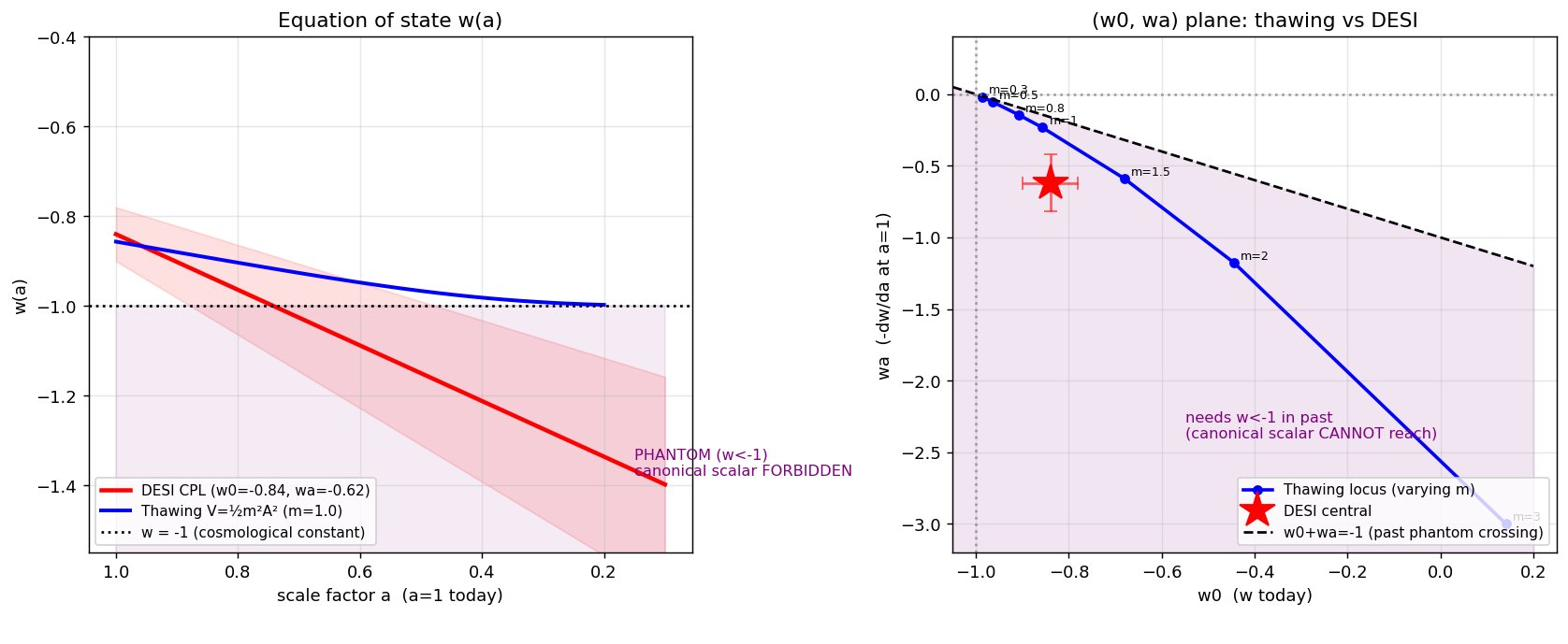
\includegraphics[width=0.99\textwidth]{afield_v1.png}
\caption{Left: $w(a)$ for thawing (blue) stays $\ge-1$; the DESI CPL line crosses below $-1$ in the past (purple, forbidden for a canonical field). Right: the thawing locus in the $(w_0,w_a)$ plane never reaches the DESI point, which sits in the past-phantom region $w_0+w_a<-1$.}
\end{figure}

% ---------------------------------------------------------------------
\section{Result 2 --- the $V\to0$ endgame (Fork Y's actual goal)}
Fork Y does not seek phantom crossing; it seeks $A\to\approx0$ ($V\to0$, Minkowski endgame). For $V=\tfrac12 m^2A^2$ (minimum at $A=0$), once $H<m$ the field is underdamped and \textbf{oscillates through} $A=0$: $A$ flips sign, $V$ touches $0$ at each crossing, and $w$ swings between $-1$ and $+1$ with $\langle w\rangle\to0$ --- i.e.\ it behaves like \emph{matter} (virial of a quadratic: $\langle K\rangle=\langle V\rangle$). \Fact\ (Turner 1983)

Integrated to $a=20.6$ (endgame demonstration run, $m=6\,H_0$, $\Omega_{\rm DE}{=}0.69$ shot at $a{=}1$ --- fast-oscillation regime, distinct from the DESI-fit $m\!\approx\!1$ scan of Result~1): the oscillation envelope decays $0.34\to0.004$; $\rho_{\rm DE}\!:2.07\to2.6\times10^{-4}$; $\rho_m\to10^{-4}$; $H\!:1.0\to0.011$. Power laws $\rho\propto a^{-3.00}$, $H\propto a^{-1.50}$, $\langle w\rangle=0.003$ --- exact matter-like dilution carrying $A\to\approx0$, $H\to0$. \Fact

\textbf{Decisive point.} $H\to0$ (not a constant) precisely because $V_{\min}=0$. Were $V_{\min}>0$, $\rho_{\rm DE}\to V_{\min}$ and $H\to$const $=$ eternal de Sitter; $V_{\min}<0$ gives recollapse (crunch). Thus $V_{\min}=0$ is exactly the choice that yields the Minkowski endgame --- and \emph{why} $V_{\min}=0$ is the Weinberg (1989) cosmological-constant wall, \Open\ for the entire field.

\textbf{Why the dark energy is thawing-class, not $\Lambda$ (conditional provenance, V3.14).} That the field rolls at all --- rather than being a bare cosmological constant --- is \emph{forced} by the endgame, not chosen to fit DESI. A true $\Lambda$ ($V\equiv\Lambda>0$) is eternal de Sitter and can reach \emph{neither} the Minkowski closure ($V_{\min}=0$, item~A) \emph{nor} the AdS one ($V_{\min}<0$, item~L); both require a field that rolls off its present value, so on those branches the dark energy \emph{must} be dynamical. (On the $V_{\min}>0$ branch a bare $\Lambda$ would serve, as in Penrose's CCC; LMU carries the dynamical $A$-field uniformly across all three.) A canonical scalar Hubble-frozen at high $z$ and only now releasing sits, by definition, in the \emph{thawing} regime --- $w\gtrsim-1$, departing from $-1$ (Caldwell \& Linder 2005; Scherrer \& Sen 2008). So the thawing \emph{class} is a corollary of the switch-off endgame, and the non-phantom $w\gtrsim-1$ that DESI tolerates at $\sim2\sigma$ (Part~II) is \emph{untuned}; the lone tuned quantity is the mass $m$ setting $w_0$ today (the why-now cost booked elsewhere in this part, not re-credited here). \textbf{Two guards against over-reading.} It forces \emph{neither} the DESI central --- a past phantom crossing $w<-1$, barred from a single canonical scalar by the $\min w=-1$ bound (Result~1; Vikman 2005) --- \emph{nor} the sign of $V_{\min}$, the open Fork (J2): $V_{\min}>0$ freezes back to de Sitter, $V_{\min}=0$ oscillates to Minkowski, $V_{\min}<0$ turns to AdS. ``Rolls to $V=0$ exactly'' is the $V_{\min}=0$ branch alone. The recombination --- Caldwell--Linder's thawing taxonomy $\times$ the cyclic switch-off requirement $\times$ the uniform-$A$-field choice --- is the LMU linkage; the thawing dynamics and the $w\ge-1$ bound are standard. \Hyp\ / \Auditor

\begin{figure}[h]\centering
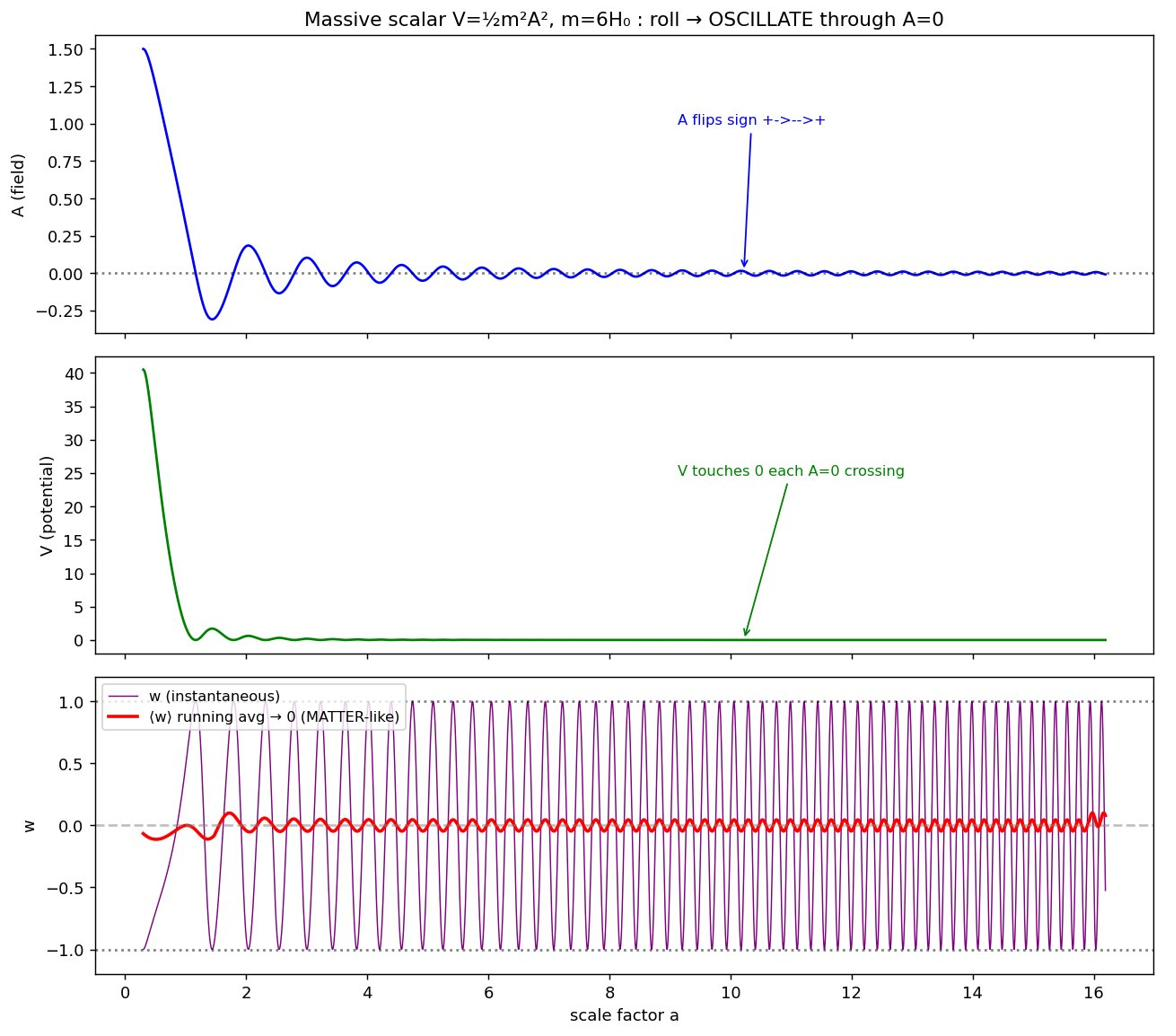
\includegraphics[width=0.92\textwidth]{afield_v2.png}
\caption{Massive scalar rolling then oscillating: $A$ alternates sign, $V$ touches $0$ at each $A=0$ crossing, $w$ swings $-1\leftrightarrow+1$, and the running average $\langle w\rangle\to0$ (matter-like).}
\end{figure}
\begin{figure}[h]\centering
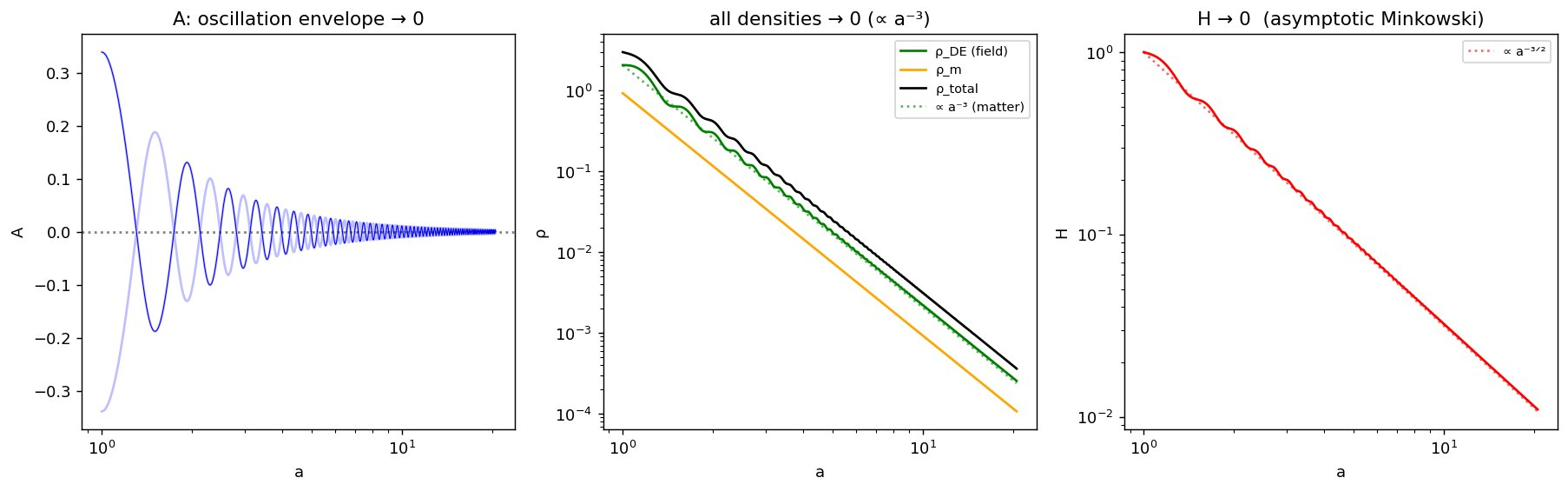
\includegraphics[width=0.99\textwidth]{afield_v3.png}
\caption{Endstate: $A\to\approx0$, all densities $\to0$ as $a^{-3}$, and $H\to0$ as $a^{-3/2}$ --- asymptotic Minkowski.}
\end{figure}

% ---------------------------------------------------------------------
\section{Result 3 --- transient acceleration (``the mountain'')}
Integrating $A$ into the future, the cosmic acceleration $\ddot a/a$ \textbf{rises, peaks, and falls} --- a transient ``mountain,'' unlike $\Lambda$CDM's plateau. Verified values of $\ddot a/a$: $a{=}0.3:-4.90$; $0.7:+0.24$; $1.0:+0.39$; $2.0:+0.16$; $4.0:-0.09$. Acceleration peaks at $a=0.99$ ($\approx$ today) and ends at $a\approx2.91$, after which the universe decelerates toward $H\to0$. \Fact

\emph{Honest caveat.} The hump is \textbf{broad and shallow} (a $\sim$7\% variation in $\ddot a/a$ across $a=0.85$--$1.2$ ($m{=}1.0$ run)), not a sharp peak; and ``we sit at the summit'' is a consequence of choosing $m$ to fit $w_0$, so the why-now coincidence is relocated into $m$, not removed.

The reason acceleration ends is that $w_{\rm tot}$ rises through $-1/3$ (equivalently $\ddot a=0$) as $A$ thaws. The CPL form must \emph{not} be extrapolated past $a=1$: with the $m{=}1.0$ scan-row $(w_0,w_a)=(-0.857,-0.233)$ (the framework's pinned joint-fit pair is $(-0.91,-0.15)$; see the F1 pin record) it gives $w(a{=}5)=+0.08$, $w(a{=}10)=+1.24$ (unphysical), whereas the real field stays bounded in $[-1,+1]$.

This transient-acceleration behaviour is published: \textbf{de Souza, Rodrigues \& Alcaniz (2025), Phys.\ Rev.\ D, arXiv:2504.16337}, who find thawing competitive with $\Lambda$CDM ($\Delta\ln B=-0.33$ vs CPL's $-1.87$) and predict acceleration ending at $z\approx-0.15$. \Fact

\begin{figure}[h]\centering
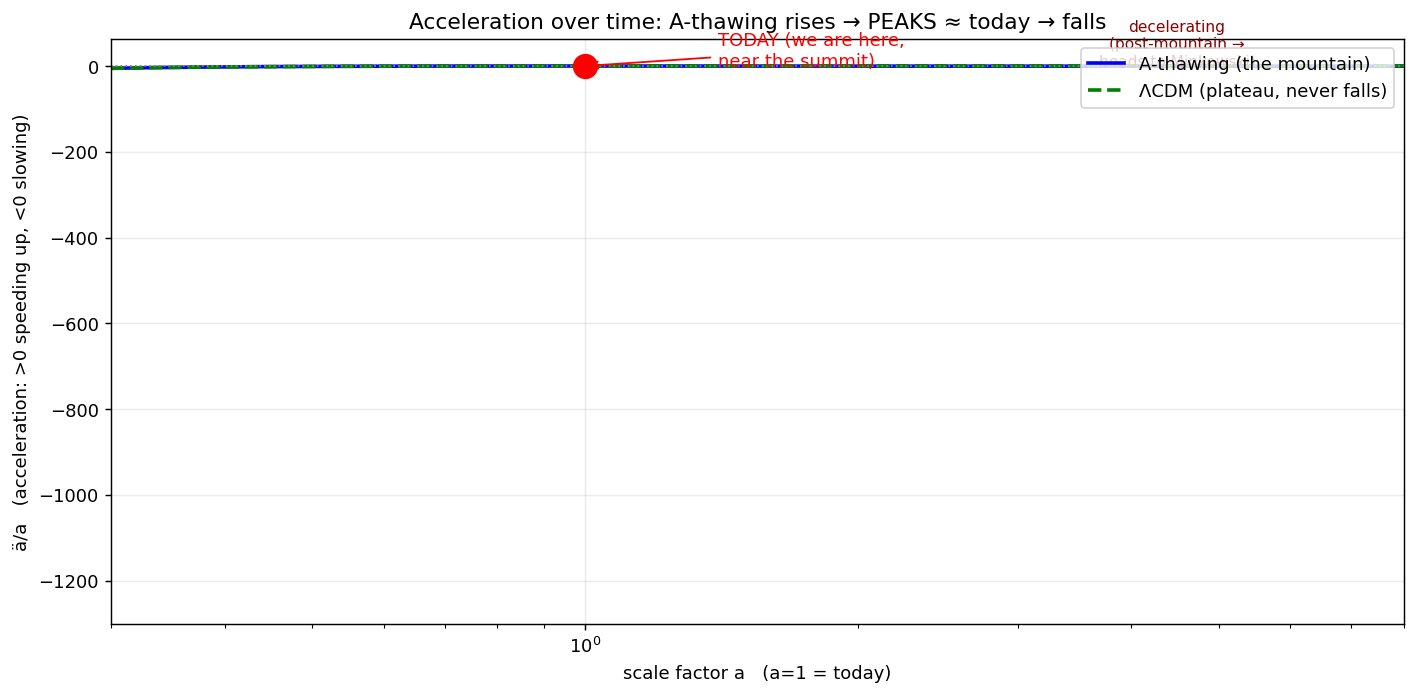
\includegraphics[width=0.95\textwidth]{afield_v4.png}
\caption{Acceleration $\ddot a/a$: A-thawing (blue) rises, peaks near today, then falls; $\Lambda$CDM (green dashed) rises to a plateau and never falls. Red dot $=$ today.}
\end{figure}
\begin{figure}[h]\centering
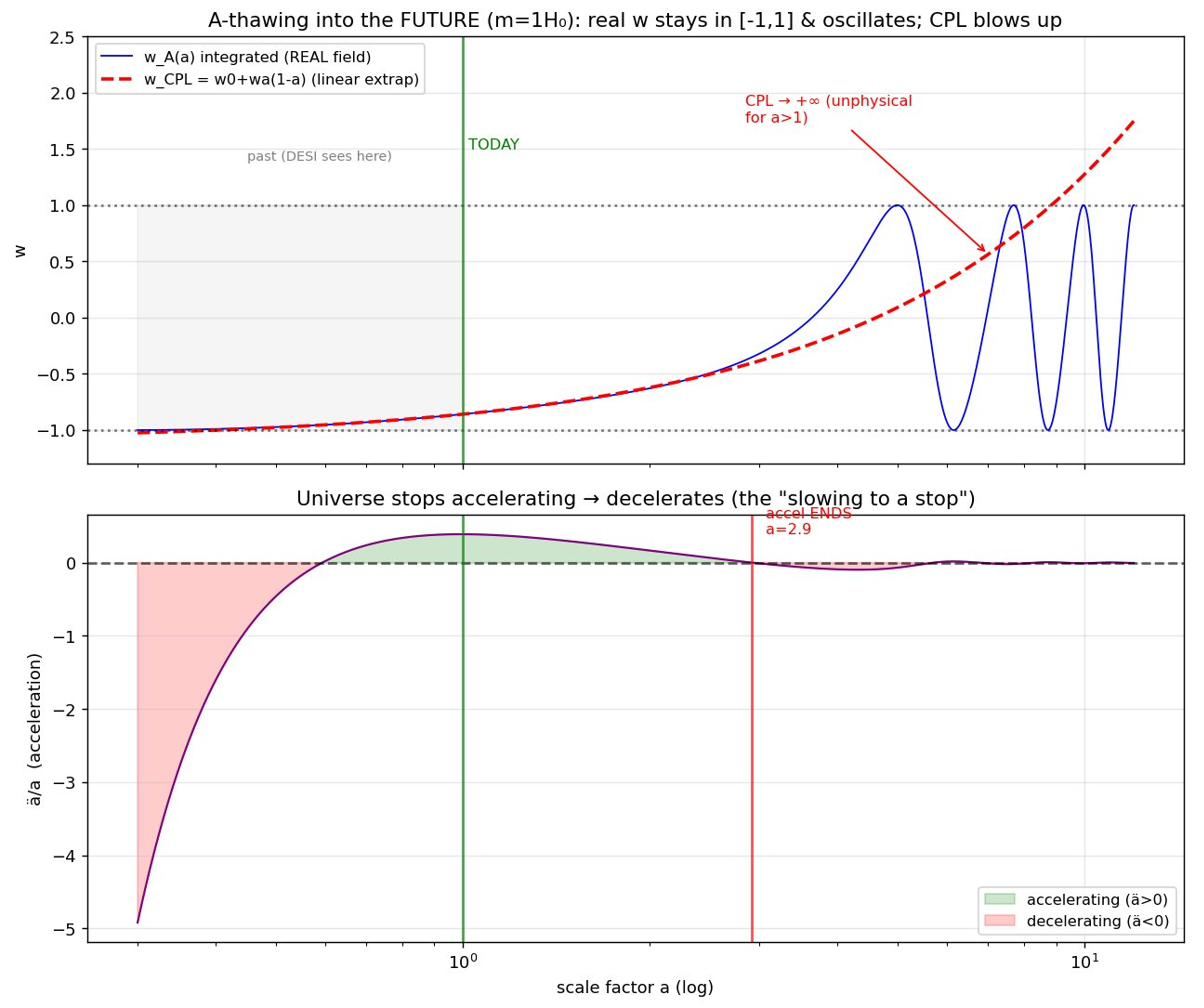
\includegraphics[width=0.88\textwidth]{afield_v5.png}
\caption{Future: the real integrated $w_A(a)$ (blue) stays in $[-1,1]$ and oscillates; the CPL linear extrapolation (red dashed) diverges and is unphysical for $a>1$. Lower panel: acceleration ends, universe decelerates (``slowing'').}
\end{figure}

% ---------------------------------------------------------------------
\section{Result 4 --- cross-check across potentials (no dialing)}
Test of robustness: pick \emph{raw} shape parameters (not chosen to hit any $w_0$), fix only the overall scale to the \emph{measured} $\Omega_{\rm DE}=0.69$, and see what comes out.
\begin{center}\small
\begin{tabular}{lccc}\toprule
potential (raw shape, no dialing) & $w_0$ (output) & $w_a$ & accel-ends $a$\\\midrule
Quadratic $\tfrac12 m^2A^2$, $m{=}1$, $A_i{=}2$ & $-0.806$ & $-0.328$ & 2.09\\
Quadratic, $m{=}1$, $A_i{=}4$ & $-0.961$ & $-0.059$ & ---\\
Exponential $e^{-\lambda A}$, $\lambda{=}1$ & $-0.847$ & $-0.191$ & ---\\
Exponential, $\lambda{=}0.5$ & $-0.962$ & $-0.053$ & ---\\
Exponential, $\lambda{=}0.3$ & $-0.987$ & $-0.019$ & ---\\
PNGB $1-\cos(A/f)$, $f{=}3$, $A_i{=}2$ & $-0.820$ & $-0.309$ & 2.18\\\bottomrule
\end{tabular}\end{center}
\textbf{What is invariant} (output, not dialed): every potential lands in $w_0\in[-0.99,-0.80]$ on the $w>-1$ side, with $w_a<0$ (thawing) and $w\ge-1$ throughout. A clear relation emerges \emph{by itself} --- $w_0$ near $-1\Rightarrow$ small $|w_a|$; $w_0\approx-0.8\Rightarrow$ larger $|w_a|$ --- i.e.\ all potentials fall on one locus in the $(w_0,w_a)$ plane. This is the signature of a canonical scalar; it appears without fitting. \Fact

\textbf{What is model-discriminating} (not rounding): the precise $(w_0,w_a)$ and the end-of-acceleration time differ with potential shape by factors of $\sim$2--3 (a quadratic with a minimum oscillates to matter and ends acceleration; a runaway exponential keeps mild negative pressure longer). These differences are real physics, and they are what observations use to tell potentials apart.

\begin{figure}[h]\centering
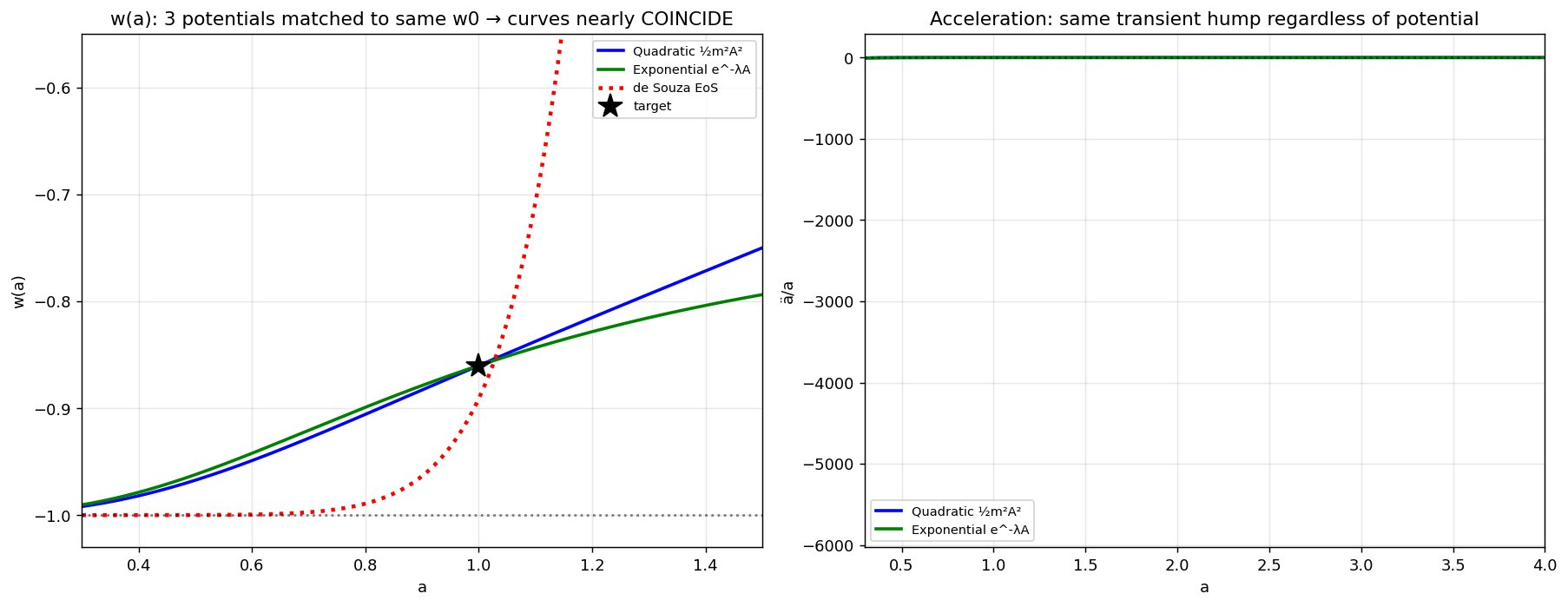
\includegraphics[width=0.99\textwidth]{afield_v6.png}
\caption{Left: $w(a)$ for several potentials (when matched in $w_0$) nearly coincide and bracket the de Souza EoS; all stay $\ge-1$. Right: all show the same transient-acceleration hump. The universal (qualitative) physics is potential-independent; the quantitative $w_a$/timing is shape-dependent.}
\end{figure}

% ---------------------------------------------------------------------
\section{Layer separation (anti-drift)}
\begin{center}\small
\begin{tabular}{@{}p{0.52\textwidth}p{0.42\textwidth}@{}}\toprule
statement & status\\\midrule
$w=(K-V)/(K+V)\ge-1$; canonical scalar never phantom & \Theorem/\Fact\\
Thawing $w(a)$, transient acceleration, $A\to\approx0$, $H\to0$ (asymptotic Minkowski) & \Fact\\
Oscillating quadratic scalar $\Rightarrow\langle w\rangle=0$ (matter-like), $\rho\propto a^{-3}$ & \Fact\\
Global energy not conserved in expansion (FRW has no time-translation symmetry) & \Fact\\
$L_0$ has an exact timelike Killing vector / exact conservation & only as $t\to\infty$; finite-time $L_0$ is \emph{quasi-static} (\Fact\ asymptotically)\\
``Island matter merges into the $L_0$ reservoir'' & \Hyp\ (LMU interpretation; not from the field equation)\\
``Entropy diluted in an infinite $L_0$ $\Rightarrow$ second-law-safe'' & \Hyp\ (rests on infinite-$L_0$; departs from Penrose)\\
``BH by-product is the source of $A$'' & \Dead\ (fails energy budget / timing / homogeneity)\\\bottomrule
\end{tabular}\end{center}
\textbf{Bottom line:} the equations deliver $A\to\approx0$, $H\to0$ (asymptotic Minkowski). ``Exact Minkowski $+$ exact conservation $+$ reservoir banking $+$ entropy dilution'' is an interpretive layer the framework adds, not a consequence of the field equation. The two must always be tagged separately. \Auditor

\textbf{Why this table is mandatory (V3.5).} It is the anti-drift guard in practice: in the session that produced Operator $B'$ it is what caught the auditor's $\Lambda$-import error (Correction~1) --- the interlude background had been computed on a constant-$\Lambda$ de Sitter despite row~2's verified $H\to0$. \Auditor

% ---------------------------------------------------------------------
\section{DESI status and the pre-registered falsifier}
DR1$\to$DR2 (6M$\to$14M redshifts): the central $(w_0,w_a)$ drifts slightly toward $-1$ while error bars shrink faster, so the preference for evolving dark energy \emph{does not diminish}; it stays $\lesssim3\sigma$, below the $5\sigma$ discovery threshold, with SN-calibration systematics unresolved, and some analyses dispute robustness. \Fact\ The thawing class is supported only at ``weak/inconclusive'' Bayesian levels but is \emph{not excluded}; non-phantom models are compatible at $2\sigma$, and the phantom-crossing evidence is the \emph{weaker} part of DESI. \textbf{V3.8 quantification (measured covariance):} on the released DR2$+$Pantheon$+$ chains $\rho(w_0,w_a)=-0.894$, and the thawing locus's minimum joint distance is $2.69\sigma$ (chain-Gaussian) / $2.40\sigma$ (posterior-mass, the convention of DESI's own $2.8\sigma$ $\Lambda$CDM exclusion, reproduced as $2.83\sigma$); the V3.7 $\rho$-grid ($2.00$--$2.92\sigma$) is retired to the pin record; ``compatible at $2\sigma$'' was the optimistic edge, and the proper test remains a direct non-CPL fit (Dinda \& Maartens 2025; de Souza et al.\ 2025). \Auditor

\textbf{V3.14 reproduction from the released chains, and an SN stress (2026-06-19).} The figures above were re-derived from the \emph{actual} DR2 posteriors rather than carried forward. The \texttt{base\_w\_wa} cobaya chains (DESI-BAO $+$ Planck NPIPE-CamSpec $+$ ACT-DR6 lensing $+$ each SN compilation) were pulled directly from the DESI Zenodo deposit (\texttt{10.5281/zenodo.16644576}); the thawing locus was re-integrated from the Part~II Klein--Gordon equations on constants alone ($\Omega_{m0}=0.31$, $H_0=1$). \emph{Method.} Each fit is scored two ways: \textbf{chain-Gaussian} --- the Mahalanobis distance of a test point to the chain mean on the chain's own $2{\times}2$ $(w_0,w_a)$ covariance --- and \textbf{posterior-mass} --- the highest-posterior-density mass enclosed at the test point, mapped to $\sigma$ through the \emph{one-dimensional} equivalence $m=\mathrm{erf}(\sigma/\sqrt2)$, the convention in which DESI quotes its $\Lambda$CDM exclusion (a two-dimensional mapping was a first, wrong, attempt; see below). For Pantheon$+$ the reproduction matches the values already committed: mean $(w_0,w_a)=(-0.838,-0.617)$, $\sigma=(0.055,0.208)$, $\rho=-0.894$. Chain-Gaussian reproduces the committed distances \emph{exactly} ($\Lambda$CDM $3.04\sigma$, thawing $2.69\sigma$); posterior-mass reproduces the committed $2.83\sigma$\,/\,$2.40\sigma$ to KDE precision (this run's getdist smoothing gives $2.78\sigma$\,/\,$2.47\sigma$, a $\sim$0.05$\sigma$ bandwidth gap). The thawing minimum sits at $m\!\approx\!0.61$, near the \emph{near-$\Lambda$} end of the locus rather than $m\!\approx\!1.3$, because the strong anti-correlation ($\rho\!\approx\!-0.9$) makes the error ellipse thin along the $w_0$--$w_a$ anti-diagonal. Stressing across the three SN compilations (the means reproduce the published DESI single-source values exactly):

\begin{center}\small
\begin{tabular}{lcccl}\toprule
DESI$+$CMB$+$ & $(w_0,w_a)$ & $\Lambda$CDM excl. & thawing-min & vs $\Lambda$CDM\\
 & & (G\,/\,post) & (G\,/\,post) & \\\midrule
Pantheon$+$ & $(-0.838,-0.62)$ & $3.04/2.83$ & $2.69/2.40$ & closer $0.3$--$0.4\sigma$\\
Union3 & $(-0.667,-1.09)$ & $3.80/3.93$ & $3.28/3.27$ & closer $0.5$--$0.7\sigma$\\
DESY5$^\dagger$ & $(-0.752,-0.86)$ & $4.33/4.39$ & $3.24/3.18$ & closer $1.1\sigma$\\
$+\,\Omega_k$ (Pan$+$) & $(-0.853,-0.54)$ & $2.61/2.14$ & $2.12/1.67$ & closer $0.5\sigma$\\\bottomrule
\end{tabular}\end{center}
\noindent{\small $^\dagger$original DESY5; the DES reanalysis lowers its $\Lambda$CDM exclusion to $\sim$3.2$\sigma$. DESI's single quoted exclusions ($2.8/3.8/4.2\sigma$) sit within $\lesssim0.2\sigma$ of these two metrics: Pantheon$+$ matches the posterior-mass figure, Union3 the chain-Gaussian, and the DESY5 quote falls just below both --- the residual is DESI's exact significance definition. Posterior-mass for Union3/DESY5/$\Omega_k$ is this run's getdist KDE ($\pm\sim$0.05$\sigma$); the Pantheon$+$ row uses the document's committed value.}

\textbf{What it shows, and how it cuts.} \emph{Robust:} canonical thawing is \emph{less disfavoured than $\Lambda$CDM in every SN compilation}, and the margin \emph{widens} where the data pull harder toward phantom (DESY5: closer by $1.1\sigma$) --- so ``closer to the data than $\Lambda$CDM'' is a property of the whole $w\ge-1$ locus against an anti-correlated posterior, not a Pantheon$+$ artefact, and it survives marginalising curvature (consistent with Dinda \& Maartens 2025). \emph{Caveat, owed to F1:} the thawing tension \emph{itself} is SN-dependent --- $2.5\sigma$ (Pantheon$+$) up to $\sim$3.3$\sigma$ (Union3)\,/\,$\sim$3.2$\sigma$ (DESY5) --- so the headline $2.40$--$2.69\sigma$ is the Pantheon$+$ (least-discrepant) number and the honest band across SN is $2.5$--$3.3\sigma$. This does \emph{not} fire the falsifier below: F1 is committed to a \emph{phantom crossing} $w(z)<-1$ at $\ge3\sigma$ with systematics resolved, and the SN-sample spread \emph{is} the unresolved systematic it conditions on; a single canonical scalar cannot cross $w=-1$ (Vikman 2005), so what moves with the SN choice is the locus's distance-to-central, never a crossing. Supersession of record: the pre-chain estimate built from the marginalised $\sigma$ alone gave $\Lambda$CDM $\sim$3.1$\sigma$\,/\,thawing $\sim$2.8$\sigma$ ($\sim$0.1$\sigma$ high); the released-chain covariance ($\rho=-0.894$) is what lands the exact $3.04$\,/\,$2.69$. Scripts \texttt{kg\_recompute.py}, \texttt{chain\_pin.py}, \texttt{stress2.py}. \Auditor

\begin{center}\fbox{\parbox{0.94\textwidth}{
\textbf{Pre-registered falsifier (committed now).} Fork Y (canonical $A$, $w\ge-1$, Minkowski endgame) is falsified \emph{iff} DESI-Y5 ($\sim$2027) sustains $w(z)<-1$ at high $z$ at $\gtrsim3\sigma$ \emph{with systematics resolved}. It is \emph{not} falsified by $w\ge-1$ evolving data, nor by a sub-3$\sigma$/systematics-limited phantom hint. The 3$\sigma$ line is fixed and must not be moved if data later push against the model.}}\end{center}

% ---------------------------------------------------------------------
\section{Run 2 --- $A_i$ fixed, $m$ shot (this session's cross-validation)}
A second, independent shooting strategy was run for the equation document (fresh KG$+$Friedmann integration, Radau): instead of fixing $m$ and shooting $A_i$ (the $m$-scan of \S2), \textbf{Run~2 fixes $A_i=2.70\,M_p$ and shoots $m$} so that $\Omega_{A,0}=0.689$. Result: $m=0.804\,H_0=1.16\times10^{-33}$\,eV; $w_0=-0.91$, $w_a=-0.15$ (matching the thawing relation $w_a\simeq-1.5(1+w_0)=-0.14$ to 4\%); acceleration window $a\in(0.61,\,5.5)$; first $A=0$ crossing at $a=9.4$ ($m$-dependent, ``few--20'' across the verified band); $\langle w\rangle\to0$ and $H\to0$ confirmed (Fig.~\ref{fig:p2afield}). Canonical $w\ge-1$ throughout. \Fact

\textbf{Cross-validation.} Run~2 lands on the $m$-scan's $m=0.8$ row, $(w_0,w_a)=(-0.908,-0.144)$ --- two independent shooting strategies ($m$ fixed/$A_i$ shot vs.\ $A_i$ fixed/$m$ shot), same point on the thawing locus. The V3.5 assembly recomputed both fresh (R6, Radau and DOP853): $A_i$ shot at $m=0.8$ gives $A_i=2.715\,M_p$, $(w_0,w_a)=(-0.9080,-0.1438)$; $m$ shot at $A_i=2.70\,M_p$ gives $m=0.8030\,H_0$, $(-0.9071,-0.1456)$. \Auditor

\begin{figure}[h]\centering
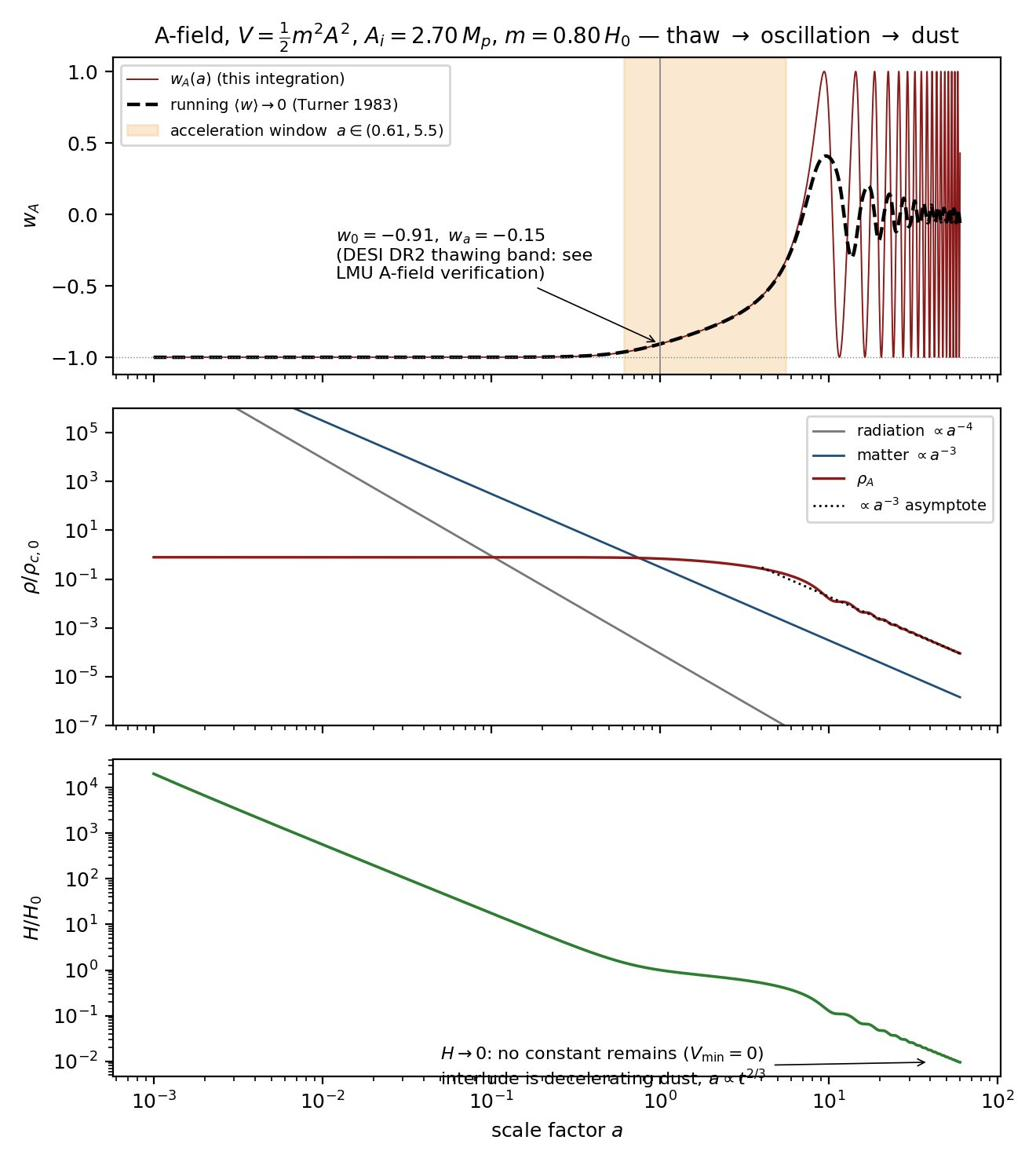
\includegraphics[width=0.86\textwidth]{fig2_afield.png}
\caption{Run 2 --- the A-field through one zone's life: thaw, transient acceleration, oscillation to dust, $H\to0$. Every curve is from the equation document's own integration (R6). Owners: eqs.~\eqref{eq:p2kg}--\eqref{eq:p2eos}, Turner 1983.}
\label{fig:p2afield}
\end{figure}

% ---------------------------------------------------------------------
\section{The PNGB cross-audit against DESI DR2 (the archived module)}
\emph{The following two sections are the consolidated worldview pass's own dark-energy module (its Part II \S\S1--2), carried as the archive record: an independent integration on a different thawing potential (PNGB rather than quadratic), in different variables (e-folds), reaching the same structural verdict. Redundancy here is deliberate --- it is the cross-check.} \Auditor

% =====================================================================
\section{The field, and what the data ask of it}
The field $A$ is a single canonical scalar with a rolling potential (Ratra--Peebles 1988; Wetterich 1988; Caldwell--Dave--Steinhardt 1998), treated \emph{per zone} rather than as a universal constant. Its job in the framework is twofold and the two are linked: it must (a) \emph{accelerate the zone now} (the only observed fact), and (b) \emph{weaken toward $A\!\to\!0$} so the zone returns to the timeless reservoir and the loop can close. DESI~DR2 sharpened (a) into a quantitative target: the data prefer an \emph{evolving} equation of state,
\begin{equation}
w(a)=w_0+w_a(1-a),\qquad w_0=-0.838\pm0.055,\quad w_a=-0.62\pm0.2\ \ (\text{DESI}+\text{Pantheon+}),
\end{equation}
i.e.\ dark energy was \emph{stronger} in the past and is weakening --- which is, qualitatively, exactly what requirement (b) predicts. The open joint O2 is whether a \emph{canonical} field (the spine the framework chose) can match this quantitatively, and which way its potential's minimum sits.

% =====================================================================
\section{Computation --- Klein--Gordon vs DESI (O2)}
The field obeys the Klein--Gordon equation in an expanding background; in e-folds $N=\ln a$, with $8\pi G=1$ and $H$ solved self-consistently from the Friedmann constraint,
\begin{equation}
\phi''+\Big(3+\frac{\dot H}{H^2}\Big)\phi'+\frac{1}{H^2}\frac{dV}{d\phi}=0,\qquad
H^2=\frac{\rho_m+V(\phi)}{3-\tfrac12\phi'^2},\qquad
w_\phi=\frac{\tfrac12 H^2\phi'^2-V}{\tfrac12 H^2\phi'^2+V}.
\end{equation}
We integrate a thawing pseudo-Nambu--Goldstone potential $V(\phi)=A_0[1+\cos(\phi/f)]$ (Frieman et al.\ 1995) --- the canonical thawing case, whose minimum sits at $V=0$ --- from a frozen high-redshift start, tuned so $\Omega_\phi(\text{today})=0.69$ with $\Omega_m=0.31$, and scan the initial displacement $\phi_0$ (how far the field thaws by today).

\begin{figure}[h]
\centering
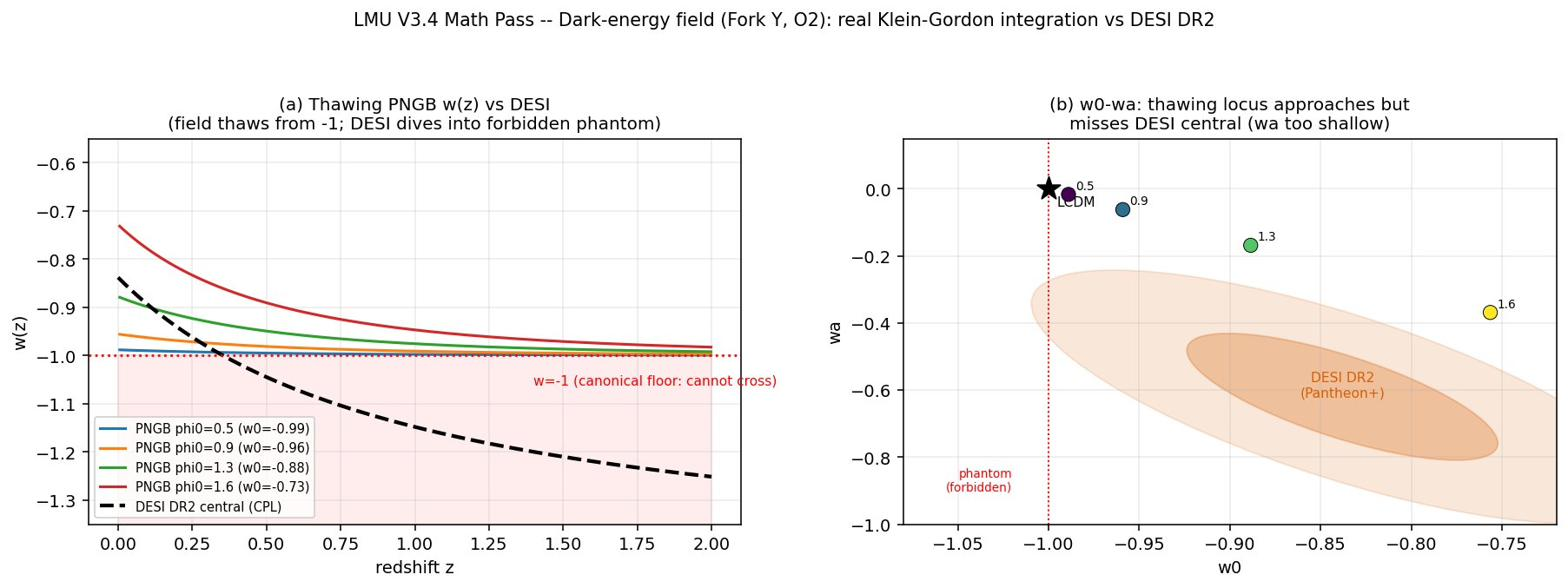
\includegraphics[width=\textwidth]{quintessence_desi.png}
\caption{\textbf{(a)} $w(z)$ for the thawing field at several initial displacements: it thaws upward from $w=-1$, while the DESI central law (dashed) dives \emph{below} $-1$ at low $z$ --- the phantom region a canonical field cannot enter. \textbf{(b)} The thawing locus in $(w_0,w_a)$: it runs from $\Lambda$CDM toward the DESI DR2 ellipse but stays above/right of the central preference --- $w_a$ too shallow, and $w_0$ overshoots before $w_a$ deepens.}
\end{figure}

\textbf{Result.} The integration reproduces, from first principles, the tension the main text states heuristically:
\begin{itemize}[leftmargin=1.3em,itemsep=2pt]
\item The thawing field reaches $w_0\!\approx\!-0.88$, $w_a\!\approx\!-0.17$ at its DESI-closest displacement --- it \emph{approaches} the data but misses the central $(w_0,w_a)=(-0.838,-0.62)$: $w_a$ is too shallow, and a canonical field \textbf{cannot cross $w=-1$} (Vikman 2005), which is where DESI's central law goes. The miss is the $\sim$2--3$\sigma$ gap the main text quotes. \emph{This is a miss of the central value, not an exclusion}: a non-phantom field ($w\ge-1$) remains compatible with DESI at $\sim2\sigma$, and the phantom-crossing signal is the weakest part of the data --- so ``cannot reach the central'' must not be read as ``ruled out as thawing.'' The honest claim is \emph{consistent at $2\sigma$}, not best-fit. \Hyp
\item \textbf{The endgame is the payoff.} The same thawing field rolls to the minimum of its potential at $\phi=\pi f$, where $V=0$ --- a Minkowski, $A\!\to\!0$ end-state, exactly the reservoir the loop needs. And the dependence runs the right way: the more the field thaws to fit DESI's evolution, the sooner it reaches $V=0$. So DESI's preference for \emph{weakening} dark energy and the framework's need for the field to \emph{switch off} are the same statement seen from two ends. \Hyp
\end{itemize}

\textbf{What it means for O2.} The field that delivers the endgame the framework requires ($V\!\to\!0$, Minkowski) is the same field that is mildly \emph{disfavoured} by the present $w_0$--$w_a$ data (too shallow, no phantom crossing). The competing reading --- the $\sim$94\% future-AdS preference in the DESI analyses --- points instead to $V_{\min}<0$, a collapsing zone, which is the rival ($f(R)$/crunch) closure rather than the reservoir. \textbf{The sign of $V_{\min}$ is therefore the whole of O2}, and it is exactly what DESI~DR3 (and Euclid/Roman) will pin down. The framework is self-consistent on the endgame it needs and is honest that today's data lean slightly the other way. \Open

\textbf{External validation and the committed falsifier.} The transient-acceleration behaviour of this field --- $\ddot a/a$ rises, peaks near today, then falls, unlike $\Lambda$CDM's plateau --- is independently published: de Souza, Rodrigues \& Alcaniz (2025, PRD, arXiv:2504.16337) find thawing competitive with $\Lambda$CDM ($\Delta\ln B=-0.33$ vs CPL's $-1.87$) and acceleration ending near $z\approx-0.15$. Honest cost: the hump is broad and shallow, and ``we sit at the summit'' follows from tuning $m$ to fit $w_0$ --- so the why-now coincidence is relocated into $m$, not removed, leaving the field even with $\Lambda$CDM on that count, not ahead. The pre-registered falsifier (fixed now, not to be moved): Fork Y is falsified \emph{iff} DESI-Y5 ($\sim$2027) sustains $w(z)<-1$ at high $z$ at $\gtrsim3\sigma$ with systematics resolved; it is \emph{not} falsified by $w\ge-1$ evolving data or a sub-3$\sigma$/systematics-limited phantom hint. The full no-dialing cross-check across six potentials (quadratic, exponential, PNGB), the $\min w=-1$ bound, the $V\to0\Rightarrow H\to0$ Minkowski endgame, and the figures are recorded in \S\S1--7 of this part (the verification record, integrated in V3.5 from the formerly separate companion document \emph{Verification of the LMU Dark-Energy Field A}); this section is the archive summary. \Fact\ / \Auditor

\subsection*{Is the DESI ``phantom past'' real, or a CPL artefact?}
This is the load-bearing question for O2, and it sharpens the falsifier above. Taking every value consistently from the DESI DR2 key paper (Abdul-Karim et al.\ 2025, arXiv:2503.14738, single source) to avoid cross-sample mixing:
\begin{center}\small
\begin{tabular}{lccl}\toprule
DESI combination & $w_0$ & $w_a$ & $\Lambda$CDM exclusion\\\midrule
DR2 $+$ Pantheon$+$ & $-0.838\pm0.055$ & $-0.62^{+0.22}_{-0.19}$ & 2.8$\sigma$\\
DR2 $+$ Union3 & $-0.667\pm0.088$ & $-1.09^{+0.31}_{-0.27}$ & 3.8$\sigma$\\
DR2 $+$ DESY5 & $-0.752\pm0.057$ & $-0.86^{+0.23}_{-0.20}$ & 4.2$\sigma\to$3.2$\sigma$ (DES reanalysis)\\
A-thawing ($m{=}1$) & $-0.857$ & $-0.233$ & ---\\\bottomrule
\end{tabular}\end{center}
Every SN combination's CPL central crosses below $-1$ in the past (at $z=0.5$, $w_{\rm CPL}\approx-1.04$ for all three samples, versus A-thawing's $-0.934$; at $z=1$ all near $-1.15$ to $-1.21$), so canonical $A$ --- pinned at $w\ge-1$ --- does not trace the CPL central for $z\gtrsim0.5$, though it agrees at $z=0$. \textbf{But this crossing is a property of the CPL straight-line ansatz, not a measurement that the field is phantom}: Dinda \& Maartens (2025, MNRAS 542 L31; arXiv:2504.15190) and de Souza et al.\ (2025, PRD; arXiv:2504.16337) show that fitting physical non-phantom thawing models (rather than CPL) gives fits comparable to CPL --- equally good on a curved background (Dinda--Maartens, whose stated conclusion is that the crossing is an artefact of a parametrization not based on a physical model) and competitive with $\Lambda$CDM ($\Delta\ln B=-0.33$, de Souza et al.) --- so the data do not enforce phantom crossing. \emph{A tension-physics caveat (hypothesis-level):} once a pre-recombination early-dark-energy component is admitted to ease the Hubble tension, a canonical evolving scalar ($w_0+w_a\ge-1$, the $A$-field's non-phantom class) becomes $1\sigma$-consistent with Planck$+$ACT$+$SPT$+$DESI$+$Pantheon$+$SH0ES (Wang \& Piao 2025, arXiv:2511.16606) --- the non-phantom class is not excluded once tension-resolving physics is on the table. The dominant systematic is the SN-sample spread ($w_0$ from $-0.84$ to $-0.67$; 2.8$\sigma$ for Pantheon$+$ up to 4.2$\sigma$ for DESY5, the latter weakened to 3.2$\sigma$ by the DES reanalysis: Popovic et al.\ 2026, MNRAS 548, arXiv:2511.07517), with Pantheon$+$ the least discrepant. So A-thawing is \emph{disfavoured at the CPL central but not excluded}, and the Y5 falsifier reduces to one sharp question: does the phantom crossing survive a physical (non-CPL) re-analysis with systematics resolved? If yes, canonical $A$ fails; if it is a parametrization artefact, $A$ stays competitive. \Open\ / \Auditor


% ---------------------------------------------------------------------
\section{Honest status}
\begin{itemize}[leftmargin=1.3em,itemsep=2pt]
\item The quintessence integration is standard scalar-field cosmology; it does not discriminate the framework from $\Lambda$CDM or from other thawing-quintessence models. Its value is to confirm O2 from a real integration and to show the endgame ($V\!\to\!0$) is realised by the DESI-approaching field.
\item The PNGB choice is representative of canonical thawing; a freezing or hilltop potential would shift $(w_0,w_a)$ and, for a hilltop, could overshoot to $V<0$ (the crunch branch) --- which is the O2 fork, not a detail.
\item The $z_{\rm aeon}$ result is an impossibility argument, not a calculation; it rests on the conformal invariance of massless-radiation entropy, which is secure, and on the boundary's scoping to the massless channel (now carried in Part~IV, Operator $B'$).
\item Everything tied to $A$ (roll rate, the sign of $V_{\min}$) remains hostage to DR3 and to the cosmological-constant fine-tuning problem (Weinberg 1989), which this module does not address. \Open
\end{itemize}


\textbf{Merged bottom line (record $+$ archive).} The equations deliver $A\to\approx0$, $H\to0$; the reservoir reading of that endgame is the framework's interpretive layer; the field's quantitative fate is left, honestly, to DESI (Y5 falsifier above). \Auditor

% ---------------------------------------------------------------------
\section{Attribution --- the dark-energy field $A$}
\begin{center}\small
\begin{tabular}{@{}p{0.45\textwidth}p{0.49\textwidth}@{}}
\toprule
Element & Owner / source \\
\midrule
Per-zone rolling field; ``$V\!\to\!0$ closes the loop'' framing & Pitarn (\Design) \\
Quintessence (rolling scalar dark energy) & Ratra \& Peebles (1988); Wetterich (1988); Caldwell, Dave \& Steinhardt (1998) \\
Thawing PNGB potential & Frieman, Hill, Stebbins \& Waga (1995) \\
No phantom crossing for a canonical field & Vikman (2005) \\
DESI DR2 $w_0$--$w_a$ constraint (single-source values) & DESI Collaboration / Abdul-Karim et al.\ (2025, arXiv:2503.14738) \\
Transient (thawing) acceleration vs DESI; Bayesian comparison & de Souza, Rodrigues \& Alcaniz (2025, PRD, arXiv:2504.16337) \\
Scant Bayesian evidence for thawing (skeptical counterweight) & Wolf, Garc\'ia-Garc\'ia, Bartlett \& Ferreira (2024, PRD 110, 083528; arXiv:2408.17318) \\
Phantom crossing as a CPL artefact; non-CPL thawing fit & Dinda \& Maartens (2025, MNRAS 542 L31; arXiv:2504.15190); de Souza et al.\ (2025; arXiv:2504.16337) \\
DESY5 recalibration weakening evolving-DE (4.2$\sigma\!\to\!$3.2$\sigma$) & Popovic et al.\ (2026, MNRAS 548; arXiv:2511.07517, ``Dovekie'') \\
Non-phantom scalar 1$\sigma$-consistent under early dark energy (hypothesis-level) & Wang \& Piao (2025, arXiv:2511.16606) \\
Conformal cyclic cosmology / massless-entropy invariance & Penrose (2010) \\
Black-hole entropy; radiation-to-BH entropy ratio ($4/3$) & Bekenstein (1973); Hawking (1975); Zurek (1982) \\
Klein--Gordon integration; conformal-boundary audit & editor pass (\Auditor) \\
\bottomrule
\end{tabular}
\end{center}

\vspace{4pt}\hrule\vspace{4pt}
{\small Module A is the dark-energy half of the math pass. It shows, from a real field integration, that the canonical thawing spine approaches but does not yet match DESI (O2, $w_0$--$w_a$ too shallow, no phantom crossing) while delivering the $V\!\to\!0$ endgame the loop requires; and it shows, from the conformal invariance of massless entropy, that the boundary's $z_{\rm aeon}$ is undeterminable in principle --- which explains the old ambiguity and confirms the framework's ``dilute, don't reset'' entropy stance. The field's fate is left, honestly, to DESI~DR3.}


\clearpage

\part{Closure of the loop --- the $L0$ ledger}
\setcounter{section}{0}\setcounter{equation}{0}\setcounter{figure}{0}

\noindent\textbf{What this module settles.} The framework's loop closes its matter, energy, and entropy budgets through a reservoir state $L0$ (a timeless, $A\!\approx\!0$, \emph{asymptotically} Minkowski background between aeons (at finite time: a quasi-static \emph{dust era}, \S2)). The verbal argument (main text \S6) is here made quantitative: what enters $L0$ and at what rate, why the energy budget balances exactly (in$=$out), where ``energy conserved'' is and is not the same as ``the loop can run,'' and --- the point of the module --- a clean separation of the \emph{four} closure worries that are answered by physics from the \emph{one} that remains an explicit, undecidable assumption. The honest end-state: the loop is closed up to a single load-bearing premise (an actually-infinite reservoir), and that premise is the toll every cyclic and eternal-inflation cosmology pays, not a defect peculiar to this one. \Design\ (the reservoir architecture and ledger) / \Fact, \Hyp\ (the physics terms) / \Open\ (the one premise).

\noindent\textbf{The substrate, in one equation (the SVT/Volovik anchor).} $L0$ is not an empty stage but the \emph{equilibrium state of the substrate}, and the framework's two axioms (a self-sustained medium, and $\Lambda$) are those of Superfluid Vacuum Theory in Volovik's $q$-theory form, which LMU adopts here as its literature home. The vacuum carries a conserved Lorentz-invariant variable $q$ (realized as Hawking's 4-form); what gravitates is the macroscopic combination, not the bare UV energy:
\begin{equation}
\Lambda=\rho_{\rm vac}=\epsilon(q)-\mu q=-P_{\rm vac},\qquad \mu=\frac{d\epsilon}{dq}.
\own{Sinha--Sivaram--Sudarshan 1975; Volovik gr-qc/0405012, 1004.0597}
\label{eq:svtlambda}
\end{equation}
In equilibrium at zero external pressure the self-tuning condition $\tilde\epsilon_{\rm vac}(q_0)\equiv\epsilon(q_0)-q_0\,d\epsilon/dq|_{q_0}=0$ forces $\Lambda=0$: the huge UV piece $\epsilon(q)\sim E_{\rm UV}^4$ (the $10^{120}$ monster) is cancelled by the $-\mu q$ counterterm \emph{without fine-tuning} (the author's ``$+/-$ neutral''). Matter, curvature, and boundaries perturb the equilibrium, giving a small $\Lambda\sim\rho_{\rm matter}$ (matter \emph{perturbs} the vacuum, it does not push --- the standing brake holds), and cosmology is the relaxation of $\Lambda$ toward $0$ as the Universe ages (the author's ``roll to $L0$''). \Fact\ (q-theory; self-tuning paper Klinkhamer--Volovik 0711.3170; bang-as-transition 2111.07962). \textbf{Sharp constraint} \factth: Volovik classifies a \emph{quadratic} $\epsilon(q)$ as the \emph{gas case} --- no cancellation, no equilibrium at zero external pressure. LMU's quintessence potential $V=\tfrac12 m^2A^2$ is quadratic, so the self-sustaining substrate $q$ must be \emph{liquid-like} (non-quadratic), \emph{distinct} from the quadratic $A$: the substrate $q$ does the $\Lambda$ cancellation, the $A$-field does the late-time $w(z)$. \textbf{Do not conflate $A$ and $q$} (the gas case loses the whole benefit). \textbf{Honest status} \Open: SVT/$q$-theory is real and peer-reviewed but a minority program (one of SUSY/anthropic/sequestering); it explains \emph{why} $\Lambda$ is small via trans-Planckian structure we do not know, not the measured number from first principles, and whether it evades Weinberg 1989 or merely relocates it is debated --- the same wall as the $V_{\min}=0$ gate (item B).

\noindent\textbf{Where Problem A may live: two phases of the $q$-substrate, not a symmetric pair (V3.22, exploratory).} The relighting fuel (Problem~A, main-text \S5) needs a high-energy metastable state to fall from. A naive reading --- a \emph{symmetric} ``$+/-$'' double-well, the two minima mirror images --- is barred by $q$-theory's own equilibrium conditions: every equilibrium $q_0$ satisfies $\rho_V(q_0)=0$, $\rho_V'(q_0)=0$, $\rho_V''(q_0)>0$ simultaneously (Klinkhamer--Volovik 1812.07046, Eq.~17), so \emph{both} floors of a symmetric well would sit at $\Lambda=0$ (two Minkowski states) and store no fuel. The fuel state must therefore be \emph{raised and not in equilibrium} --- an asymmetry, not a mirror. The literature supplies exactly this in two independent ways. \factth\ (i)~$q$-theory finds that a dynamical solution of the cosmological-constant problem \emph{requires} a high-energy de~Sitter vacuum that \emph{decays} to the Minkowski equilibrium (``the decay of the de-Sitter vacuum is a necessary condition''; Klinkhamer--Savelainen--Volovik 1601.04676) --- i.e.\ the substrate already carries a raised de~Sitter state above its $L0$ floor, and that state must relax downward. A flash-triggered decay of that raised state into the Minkowski basin \emph{is} the B-primary relighting, read in $q$-language. The explicit $q$-language calculation now exists: Klinkhamer--Santill\'an--Volovik--Zhou (2019, \emph{Physics} \textbf{1}, 321, arXiv:1901.05938) numerically evolve a finite-region bang surrounded by an infinite equilibrium-Minkowski vacuum --- their own ``the Big Bang takes place not over the whole of space but only in a finite region, surrounded by equilibrium Minkowski vacuum'' is LMU's flash-in-$L0$ in $q$-language, set on the same $\rho_V(q)=\epsilon(q)-\mu q$ double-well [their Eqs.~(7),(10),(14)] --- and Volovik (2023, arXiv:2312.02292) supplies the matching reheat channel (a de~Sitter phase carries a thermal bath at $T=H/\pi$, so it creates matter, heats, and decays). \textbf{Caveat} \Auditor: their $q$-bubble runs the transition in the \emph{opposite} energy direction --- $q_1$ inside, dispersing the released $\Delta V$ outward to infinity (their interest being how $\Lambda\!\to\!0$), where LMU instead keeps that $\Delta V$ as the bang's heat --- the same downhill curve $q_1\!\to\!q_0$, opposite energy fate; the scaffold (the double-well and its equilibrium triple) is shared, the energy bookkeeping is not. \factth\ (ii)~the substrate, realized as a plastic fermionic ``vacuum crystal,'' admits \emph{distinct nontrivial topological phases} (Klinkhamer--Volovik 1812.07046), so the ``two states'' are most naturally two phases separated by a transition, not two points of one analytic potential. \textbf{Anti-drift caveat} \factth: $q$-theory's worked crossover example generates only a \emph{small} remnant $\Delta\Lambda\sim E_{\rm ew}^{8}/E_{\rm Planck}^{4}$ at the \emph{electroweak} scale $E_{\rm ew}\sim10^{3}$\,GeV (Klinkhamer--Volovik) --- this is a proof that a phase crossover \emph{can} leave a residual vacuum energy, \emph{not} a derivation of a GUT-scale ignition fuel; the scale a hot start needs ($\sim10^{16}$\,GeV) is not delivered by that example and remains to be supplied. The pay-off, taken only this far, is economy and provenance: the substrate's $\Lambda$-cancellation and the inflaton-level false vacuum $\Phi_{\rm gen}$ (Layer~C) need not be two independent posits --- a single $q$-substrate with a raised, decaying de~Sitter phase can host both, folding $\Phi_{\rm gen}$ into $q$. \textbf{Problem~A is relocated, not resolved} \Open: $q$-theory itself states the Minkowski endgame ``still requires fine-tuning of the initial conditions'' (1601.04676), so ``why the substrate starts in / accesses the raised phase at the right scale'' is exactly the open posit, now worn as a phase/initial-condition question rather than a free-floating false vacuum --- the same Weinberg (1989) wall the substrate anchor already names, in topological-phase dress. \Hyp\ / \Design\ (the two-phase reading; the de~Sitter-decay and topological-phase facts are Klinkhamer--Volovik's, the LMU use is the wiring; Problem~A unchanged)

% =====================================================================
\section{The reservoir and what enters it}
Let a single zone (one causally bound island) end its aeon. Three channels route its mass--energy into the shared reservoir $L0$ --- but at different stages: one evaporates \emph{in} $L0$ (after the zone has relaxed toward Minkowski --- the dust era, \S2), one fires \emph{inside} the still-accelerating zone with its radiation entering $L0$ only as the zone relaxes, and one simply drifts in. All three are standard physics, assembled by Pitarn into one ledger.

\textbf{(1) The survivor evaporates (the slow source).} The lone L1, having swept its reach and spun down (Page 1976, which reaches $a_\ast\!\to\!0$ \emph{before} the end), evaporates by Hawking radiation. For a hole of mass $\Mbh$ the temperature, luminosity, and lifetime are
\begin{equation}
T_H=\frac{\hbar c^3}{8\pi G \Mbh k_B},\qquad
L=\frac{\hbar c^6}{15360\,\pi\,G^2 \Mbh^2},\qquad
\tau_{\rm evap}=\frac{5120\,\pi\,G^2 \Mbh^3}{\hbar c^4}\simeq 2.1\times10^{67}\Big(\frac{\Mbh}{\msun}\Big)^{3}\ {\rm yr}.
\label{eq:hawking}
\end{equation}
For a survivor at the canonical band top, $10^{11}\,\msun$: $\tau_{\rm evap}=2.1\times10^{100}$~yr and $S_{\rm BH}=1.05\times10^{99}\,k_B$ (a $10^{12}\,\msun$ \emph{upper illustration} gives $T_H\!\sim\!6\times10^{-20}$~K, $\tau_{\rm evap}\!\sim\!2\times10^{103}$~yr): the survivor is not a one-off blast but a \textbf{slow, cold bleed of its full rest energy $\Mbh c^2$ into $L0$ over an enormous time}. Because the interlude background is a \emph{decelerating dust era} with no event horizon (\S2), this slow bleed is not a loss channel: radiation not yet re-gathered dilutes only power-law (number density $a^3\sim10^{180}$ per interlude; energy $a^4\sim10^{240}$) while matter \emph{clusters} on a far faster clock (the race, \S2 and \S4), and a not-yet-evaporated hole is itself a standing mass that anchors where the next structure can grow. \Fact\ (Hawking 1975; lifetime as quoted).

\textbf{(2) Ceiling-limited holes pop (the fast source) --- a \emph{within-zone} event.} While a zone is still accelerating ($A>0$, an effective de Sitter phase with Hubble rate $H$), a black hole cannot exceed the Nariai mass, set by the merging of the black-hole and cosmological horizons in Schwarzschild--de Sitter geometry. The degenerate-horizon condition $9G^2M^2\Lambda/c^4=1$ (with $\Lambda=3H^2/c^2$) gives
\begin{equation}
M_{\rm Nariai}=\frac{c^3}{3\sqrt3\,G H}\ \approx\ 1.7\times10^{22}\,\msun\quad(H\!\sim\!H_0),
\label{eq:nariai}
\end{equation}
not the naive ``hole the size of the Hubble radius'' value $c^3/(2GH)$, which overestimates the coefficient by $\sqrt{27}/2\!\approx\!2.6$. A hole that reaches this ceiling before it can evaporate decays by the Nariai instability into radiation (Route A). \emph{This happens inside the zone, not in $L0$:} once the zone relaxes to $A\!\approx\!0$ there is no cosmological horizon ($H\!\to\!0\Rightarrow M_{\rm Nariai}\!\to\!\infty$), so there is no Nariai ceiling in the reservoir itself --- the pop is a de Sitter-phase event whose radiation enters $L0$ only as the zone winds down. \Hyp\ (Nariai 1950; instability: Ginsparg \& Perry 1983; Bousso \& Hawking 1996 --- the post-Nariai fate is less established.)

\textbf{(3) Debris escapes as $A\!\to\!0$ (the cold source).} Mass not bound into the survivor --- mid-aeon ejecta, un-captured outskirts (the two ejection routes of the ladder) --- is left adrift as the zone relaxes to Minkowski, and drifts into $L0$ carrying its rest mass. This is the \emph{material} that seeds later rounds (it has a genuine past; it is not a vacuum fluctuation). \Hyp

Crucially, by unitarity the evaporation leaves \emph{no} remnant: the entire $\Mbh c^2$ is returned to the exterior as radiation \factth. So a zone's collapsed mass is \textbf{not} lost down a hole --- it re-emerges in $L0$.


% =====================================================================
\section{The interlude background --- a dust era (Correction 1)}
\emph{(New in V3.5, from the Operator-$B'$ session; the constant-$\Lambda$ interlude of earlier drafts is retired --- Part~V \S4.)} After oscillation onset (Part~II \S3) the zone and its surroundings are a \textbf{dust universe}:
\begin{equation}
a\propto t^{2/3},\qquad H=\frac{2}{3t}\;\to\;0,\qquad\text{no event horizon}
\label{eq:dustera}
\end{equation}
(\Fact, FRW dust). Over one interlude ($\tau=2.1\times10^{100}$\,yr at the $10^{11}\,\msun$ band top, eq.~\eqref{eq:hawking}) the comoving causal reach is $\sim8\times10^{56}$\,m $\approx10^{27}$ island radii; mean densities dilute by $a^3\sim10^{180}$ (matter) while structure \emph{grows}:
\begin{equation}
\delta\propto a^{p},\quad p=\frac{-1+\sqrt{1+24f}}{4}\ \ (f=\text{clustering fraction});\qquad
t_{\rm coll}\simeq t_{\rm osc}\Bigl(\frac{1.686}{\delta_i}\Bigr)^{3/2}
\label{eq:gunngott}
\end{equation}
(\Fact: linear growth in a mixed background; Gunn--Gott 1972). And the live-phase Nariai ceiling does not operate here: $M_{\rm Nariai}=c^3/(3\sqrt3\,GH)\to\infty$ as $H\to0$ --- eq.~\eqref{eq:nariai} is a de Sitter-window statement only.

$\hookrightarrow$ \textbf{Couplings and results.} (i) Pair collapse beats evaporation by $\sim\!10^{89}$ for $\delta_i\sim1$ (Fig.~\ref{fig:race}; this assembly's R6 run gives $10^{89\text{--}90}$ at $\delta_i\sim1$ and still $10^{85}$ at $\delta_i=10^{-3}$): survivor--survivor mergers and corpse aggregation are \emph{generic}; the cross-island forced fork (same merger map, $S(2M)=4S(M)$) is the main channel, not the exotic branch. (ii) The aggregation \emph{rate} is now \textbf{computed} (item F, resolved 2026-06-10; Fig.~\ref{fig:jeansgate}): the two branches are \emph{scale}-separated by the field's Jeans length. Below the comoving $\lambda_J=1.68\times10^{26}$\,m $=0.38\,R_{\rm obs}$ at oscillation onset (shrinking $\propto a^{-1/4}$; Hu--Barkana--Gruzinov 2000), the A-dust is pressure-supported: with the Part~II late-time $\rho_A/\rho_m=63$ the clustering fraction is $f=0.016$, $p=0.044$, growth $\times\!\sim\!4\times10^2$ per interlude --- nearest neighbours still merge. On island scales the A-dust is \textbf{super-Jeans from onset} ($R_{\rm isl}/\lambda_J=2.9\times10^3$ at the live $m=0.803\,H_0$, the margin growing as $a^{1/4}$; oscillating scalar as dust, Turner 1983): $p\to1$ and the hierarchy runs open. The gate over the field mass closes only at $m\lesssim0.13\,H_0$ --- by \emph{horizon exile} ($>$100 e-folds of late slow-roll inflation, $N\approx A_i^2/4$, Linde 1983), not Jeans pressure --- a regime already excluded by the model's own DESI-thaw identification; island modes re-enter at $a/a_{\rm osc}=2.6\times10^7$ and any seed $\delta\gtrsim10^{-52}$ collapses before $\tau$, while the Poisson discreteness floor alone ($\delta\sim6\times10^{-11}$; Afshordi--McDonald--Spergel 2003 analog) exceeds the requirement by $\sim\!10^{42}$. \factth\ (conditional on $V_{\min}=0$, item B; seed origin stays open in item D) (iii) New zones are born at aggregation sites (``where the material has gathered''), which restores the author's gathering picture with a physical mechanism. \Hyp\ riding fork 5.

\textbf{Underpinning.} A BH--BH merger conserves no horizon area downward: $A_{\rm final}\ge A_1+A_2$ (Hawking area theorem, 1971; confirmed empirically by GW250114 --- LVK, PRL 135, 111403 (2025) --- where the remnant horizon area exceeds the sum of the progenitor areas to high credibility), the classical floor beneath the entropy doubling $S(2M)=4S(M)$ used in the climb. The smaller hole crosses the larger horizon whole (no remnant, no-hair); the merger energy leaves as gravitational waves ($\sim$5--10\% of rest mass, to infinity), distinct from accretion ($\sim$10--40\%, radiated locally --- the AGN-feedback term, Salpeter 1964; Lynden-Bell 1969). Both are \emph{conversion} of already-swallowed mass, not creation, and neither is dark energy (A2). \Fact



\begin{figure}[h]\centering
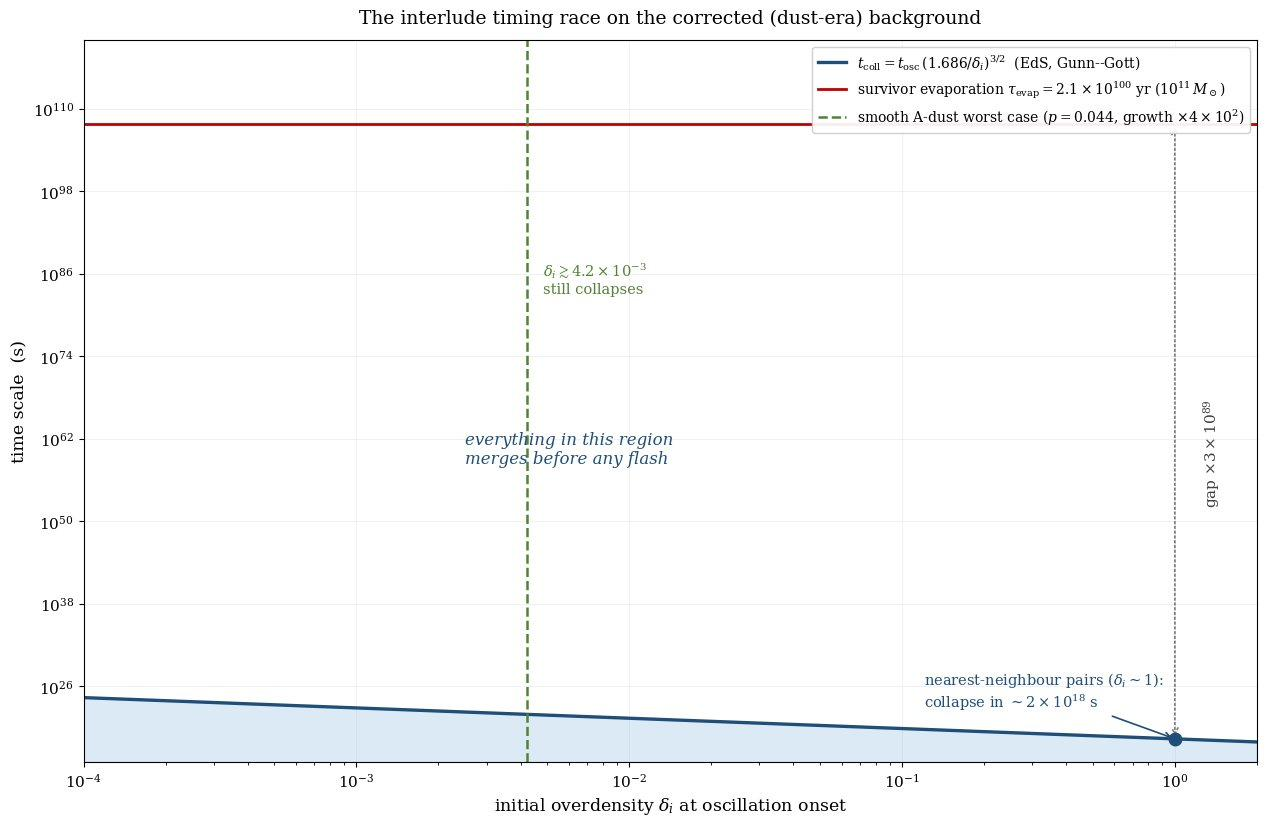
\includegraphics[width=0.8\textwidth]{fig3_race.png}
\caption{The interlude timing race on the corrected background. Everything in the shaded region merges before any flash. The dashed line marks the smooth-A-dust worst case --- now scoped to sub-Jeans scales only; island scales cluster (item F, Fig.~\ref{fig:jeansgate}).}
\label{fig:race}
\end{figure}

\begin{figure}[h]\centering
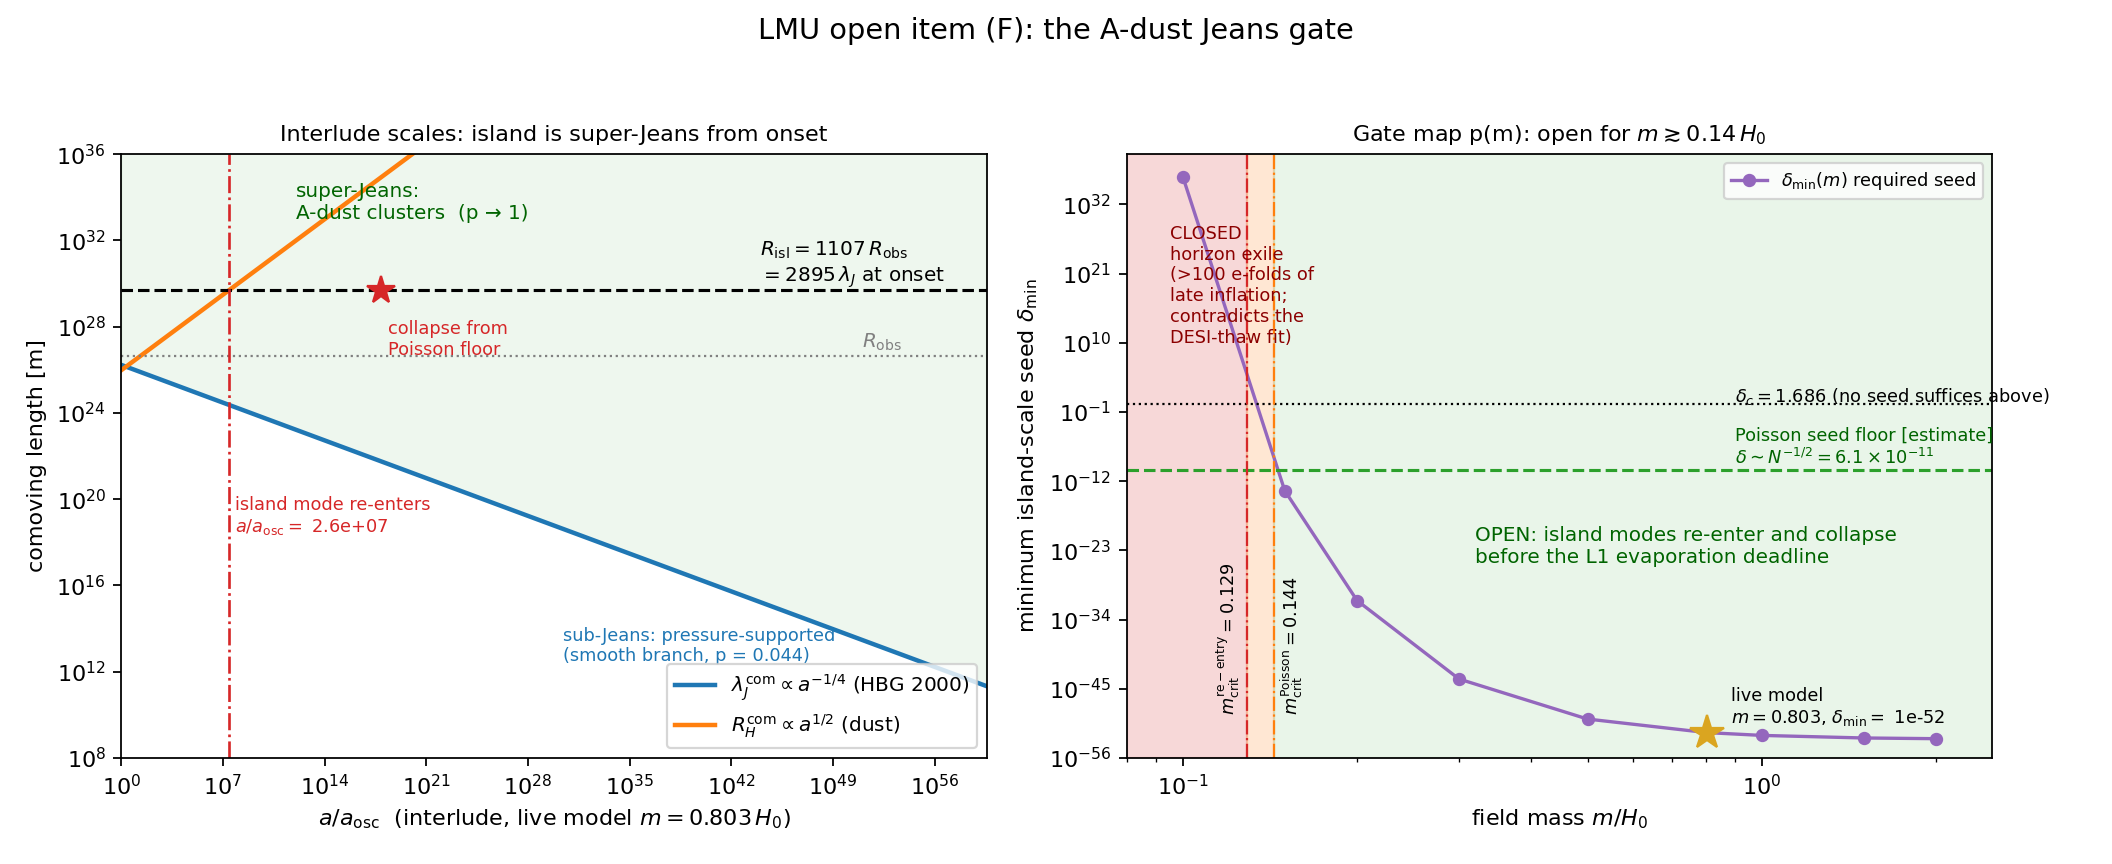
\includegraphics[width=0.99\textwidth]{lmu_itemF_jeans_gate.png}
\caption{Item F resolved. \textbf{Left:} comoving scales over the live interlude --- the island bound $R_{\rm isl}=1107\,R_{\rm obs}$ sits a factor 2896 above $\lambda_J$ at onset and the margin grows ($\lambda_J^{\rm com}\propto a^{-1/4}$); island modes re-enter the horizon at $a/a_{\rm osc}=2.6\times10^7$ and collapse from the Poisson floor long before $\tau$. \textbf{Right:} the gate over the field mass --- $\delta_{\min}(m)$ versus the Poisson seed floor; open for $m\gtrsim0.14\,H_0$, closed below $\approx0.13\,H_0$ by horizon exile (a regime outside the DESI-thaw identification). Reproduced by \texttt{lmu\_itemF\_jeans\_gate.py}.}
\label{fig:jeansgate}
\end{figure}

% =====================================================================
\section{Energy balances exactly --- the in$=$out ledger}
\textbf{Why conservation holds here, and not inside a live zone.} General relativity has \emph{no} global energy-conservation law in a generic expanding spacetime --- there is no timelike Killing vector, and a photon's energy redshifts away with no local sink (this is why ``energy is not conserved'' in an accelerating zone with $A>0$). The reservoir is the exception \emph{asymptotically}: $L0$ tends to $A\!\approx\!0$, i.e.\ Minkowski as $t\!\to\!\infty$, which \emph{does} admit a timelike Killing vector $\xi^\mu=(\partial_t)^\mu$, and hence a conserved total energy
\begin{equation}
E_{L0}=\int_{\Sigma} T_{\mu\nu}\,\xi^{\mu}\,n^{\nu}\,d\Sigma\;=\;{\rm const}.
\label{eq:killing}
\end{equation}
Per the layer-separation table (Part~II \S6), the exact Killing vector and exact conservation hold \emph{only asymptotically}; the finite-time interlude is a quasi-static dust era (\S2) with $H=2/(3t)\to0$, and the conservation statement is its $t\to\infty$ limit, used as the bookkeeping frame. \Auditor\ This is the firm ground under Pitarn's ``in$=$out'': conservation is asserted \emph{at the reservoir level}, where the symmetry that guarantees it actually exists, not across the conformal boundary and not inside an expanding zone.

\textbf{The ledger.} Summing the three channels, each zone deposits its rest energy $E_{\rm zone}\simeq\sum_i M_i c^2$ into $L0$ (channels 1--2 as radiation, channel 3 as rest mass); the reservoir in turn feeds the assembly of new zones. At the level of the whole reservoir, with $\dot E^{\rm in}_{L0}$ the rate of deposit from dying zones and $\dot E^{\rm out}_{L0}$ the rate drawn into forming ones,
\begin{equation}
\boxed{\ \dot E^{\rm in}_{L0}=\dot E^{\rm out}_{L0}\quad\Longleftrightarrow\quad E_{L0}=\text{const (closed reservoir).}\ }
\label{eq:inout}
\end{equation}
This is an \emph{accounting identity given closure}, not a theorem proved from below: it holds \emph{if} $L0$ is a closed system (nothing leaks beyond it). ``$L0$ is closed'' is the same statement as ``$L0$ is all there is'' --- i.e.\ the infinite-reservoir premise of \S6. So \eqref{eq:inout} is exact, but it names the assumption it rests on rather than removing it. \Auditor\par\textbf{V3.7 boundary scope:} \eqref{eq:inout} is the \emph{$L0$ debris channel only}. Across the conformal boundary the \emph{energy} ledger does not close: per child, the pre-rescale flash share is $\sim3\times10^{60}$\,J against a child matter content $\sim2\times10^{80}$\,J today, so every crossing injects a factor $\Omega\sim10^{26}$ (pair threshold) to $10^{43\text{--}47}$ (GUT gluing) --- permitted by GR (no global conservation off the Killing frame), supplied by nothing, identical to the irreducible $z_{\rm aeon}$ of Part~IV \S2. The photon-count/entropy closure across the boundary is an \emph{identity} (bookkeeping), not a test. \Auditor\par\textbf{Ledger principle (V3.9, author):} \emph{nothing is lost without a receipt} --- every LMU ledger either closes exactly (entropy per comoving patch, B1$'$; local $\nabla_\mu T^{\mu\nu}=0$), is reset by declaration (the B3$'$ re-init list: baryon number via the Sakharov conditions, DM, $A_i$, $P(k)$, $\Omega_k$), or carries a named price (the $\times\Omega$ boundary injection; $T_{\rm reheat}$). No silent channel exists; ruling (a) extends the closed entropy ledger to the past direction (finite aeon depth per tree).

% =====================================================================
\section{Energy is not the same as usable capacity}
The ledger \eqref{eq:inout} closes the \emph{energy} budget. It does \emph{not}, by itself, guarantee the loop can keep running, because heat death was never about energy disappearing --- it is about \emph{usable capacity} (the ability to build structure) degrading while energy is conserved. The relevant question is whether radiation deposited cold in $L0$ can be \emph{re-gathered into mass} to seed a new round.

Re-formation needs a region driven back above the relevant production threshold; for $e^+e^-$ this is
\begin{equation}
k_B T \gtrsim 2 m_e c^2 \;\Rightarrow\; T\gtrsim 1.2\times10^{10}\ {\rm K},
\label{eq:pair}
\end{equation}
reached only where gravity re-concentrates the diluted radiation to high density (mass leads, radiation follows; main paper \S12.4). The loop's \emph{capacity} therefore closes only if the reclamation rate keeps pace with dilution,
\begin{equation}
\Gamma_{\rm reclaim}(\text{gravity re-concentration})\ \gtrsim\ \Gamma_{\rm dilute}(\text{drift, redshift in }L0),
\label{eq:net}
\end{equation}
in the net over infinite time. \textbf{This inequality is now quantified} on the corrected dust background (\S2): Gunn--Gott collapse, eq.~\eqref{eq:gunngott}, beats the survivor's evaporation clock by $\sim\!10^{89}$--$10^{90}$ at $\delta_i\sim1$ and still by $\sim\!10^{85}$ at $\delta_i=10^{-3}$ --- generic, not marginal --- so \eqref{eq:net} holds wherever \emph{any} component clusters. The aggregation-rate gate is now \textbf{resolved} (item F): sub-Jeans scales keep the suppressed branch ($f=0.016$, $p=0.044$, $\times\!\sim\!4\times10^{2}$ --- nearest neighbours still collapse); island scales are super-Jeans from onset and run the hierarchy open ($p\to1$) for every $m\gtrsim0.14\,H_0$, the closed branch ($m\lesssim0.13$, horizon exile) lying outside the live model (\S2, Fig.~\ref{fig:jeansgate}). Status: the inequality \eqref{eq:net} is \Hyp\ (\emph{quantified}); the rate gate is closed in the live model, \factth\ conditional on $V_{\min}=0$; the remaining role of the infinite-reservoir premise (next sections) is capacity-\emph{forever}, not capacity-per-interlude. \Open\ (capacity only) \textbf{V3.7 exchange rate:} with the measured $g=4.0\times10^{14}$, colonization must supply $10^{14.6}$ fresh island volumes per generation; any \emph{finite} $L0$ of $10^{X}V_{\rm isl}$ is exhausted after $n_{\max}=X/14.6$ generations ($10^{3}\to0.2$; $10^{100}\to6.8$; $10^{1000}\to68.5$) --- ``large'' buys $\log_{10}/14.6$ rounds; only actually-infinite runs forever. \Auditor

% =====================================================================
\section{Four worries answered by physics}
Stated together so the contrast with the one remaining premise is clean. Each is closed by a mechanism with an owner, not by assumption.
\begin{itemize}[leftmargin=1.35em,itemsep=3pt]
\item \textbf{Energy loss --- closed.} Unitary Hawking evaporation returns the full $\Mbh c^2$; no remnant, no hole swallows energy permanently; $L0$'s Minkowski Killing vector \eqref{eq:killing} conserves the total. Energy in$=$out. \Fact
\item \textbf{Boltzmann brains --- closed.} The seeds of a new round are \emph{real debris with a past} (channel 3), not vacuum fluctuations. A \emph{material} floor does not over-produce freak observers the way a fluctuation floor would ($P\!\propto\!e^{-\Delta S}$ favours a lone brain over a universe only when the floor is fluctuational). The framework's floor is material, so the reductio that kills fluctuation-based eternal cosmologies does not bite. \Hyp
\item \textbf{Classical heat death (uniformity) --- closed.} Gravity is not gas-in-a-box: a self-gravitating system has negative heat capacity and \emph{no} maximum-entropy equilibrium (Antonov 1962; Lynden-Bell \& Wood 1968, the gravothermal catastrophe). Smoothness is maximally unstable (Jeans), so a near-still state is the most unstable starting point, not a dead end --- the perturbation that restarts the engine is a theorem, not a hope. \Fact
\item \textbf{Running down to zero --- closed.} Rounds are not one tank draining on a global clock; they are born at \emph{different places} in an unbounded volume, each with its own cycle. There is no global time along which a per-round rate declines; ``Goldilocks always available \emph{somewhere}'' replaces ``the reservoir slowly empties.'' \Hyp
\end{itemize}

% =====================================================================
\section{The one assumption that remains}
What all four resolutions quietly use --- and what \eqref{eq:inout} and \eqref{eq:net} reduce to --- is a single premise:
\begin{equation}
\boxed{\ L0\ \text{is genuinely infinite (or growing), with low-density ``Goldilocks'' regions always remaining.}\ }
\end{equation}
If $L0$ were merely \emph{large} but finite, the deposit sites would be finite, every region would eventually thermalise, and the running-down worry would return. The whole structure rests on \emph{infinite}, not \emph{large} --- and whether space is actually infinite is unmeasurable in principle (the observable horizon is finite; everything beyond is assumption).

\textbf{Why this escapes the standard no-go results.} The Borde--Guth--Vilenkin theorem makes a spacetime of net positive average expansion past-incomplete; the dust-era endgame gives $H_{\rm avg}\to0$, so the BGV premise can \emph{fail asymptotically}, and the Aguirre--Gratton construction is the documented route through it --- past-eternity is now an \emph{adopted} axiom-level choice (item H, decided 2026-06-10; the explicit per-patch construction remains open as item H1, entangled with item A); forward-eternity is free (branching $\ge1$). The Kinney--Stein bind --- that zero average expansion leaves no expansion with which to dilute the accumulating entropy --- is then escaped \emph{not} by expansion but by the infinite reservoir itself: the entropy density
\begin{equation}
\rho_S=\frac{S_{\rm total}}{V_{L0}}\to 0\qquad(V_{L0}\to\infty)
\end{equation}
falls even though $S_{\rm total}$ rises every round (second-law-safe). \emph{This is precisely why the infinite-$L0$ premise, not an entropy reset, is the load-bearer.} \Open\ (BGV: Borde, Guth \& Vilenkin 2003; the bind: Kinney \& Stein 2021, arXiv:2110.15380.)

\textbf{The rate of the bill is measured, not bounded (V3.5).} The per-round entropy growth factor $g=(4/3)\,\Sigma S_{\rm BH}/S_{\rm bath}$ is \emph{intensive} --- an entropy-density ratio that island size cannot tune --- and is now measured: floor $1.7\times10^{13}$ (BHMF holes $\ge10^9\,\msun$ only), fiducial $\mathbf{4.0\times10^{14}}$ (Egan \& Lineweaver 2010 budget), post-ladder $\sim\!2\times10^{16}$ (assumption-dependent; V3.7 recompute: $7.4\times10^{16}$, Part~VII \S1 --- OoM-stable). Behind the demographics: Soltan 1982; Marconi \& Hunt 2004; Shankar, Weinberg \& Miralda-Escud\'e 2009. \Fact\ (the measurement; details Part~IV \S1)
\begin{center}\fbox{\parbox{0.92\textwidth}{\centering \textbf{Fork-5 condition (background-independent counting):} the population must colonize fresh comoving extent at $\ge(1+g)\approx10^{14.6}$ per generation, forever $\iff$ \textbf{$L0$ unbounded}. Kill: any finite $L0$, or sub-exponential capacity.}}\end{center}
The old bound $g\in(0,10]$ and its $\times2$/round kill figure are \textbf{retired} (Part~V \S4); the premise above is unchanged --- what changed is that its price per generation is now a number. \Auditor

% =====================================================================
\section{Entropy --- diluted, not reset (and why it cannot be reset)}
\noindent\Auditor\ \textbf{[B-alt argument; the dilution conclusion is route-agnostic.]} The \emph{conclusion} --- the second law's debt is paid by dilution in the infinite $L0$ reservoir --- holds under either joint (Layer~A). The \emph{argument} below, that the conformal rescale cannot reset entropy because massless-radiation entropy is conformally invariant, is specific to the alternative joint (B-alt): it is a constraint on the rescale. Under the primary joint (B-primary nucleation) there is no rescale to reset anything, so the question does not arise --- old $L0$ radiation entropy simply dilutes while each freshly nucleated pocket reheats at low entropy.
The premise above also fixes how entropy is handled, and a companion result (Part~IV \S2) shows the alternative is closed off: the survivor's terminal radiation is massless, and the entropy of massless radiation is \emph{conformally invariant} (photon number is preserved under $g\!\to\!\Omega^2 g$). The Penrose rescale that lights the next hot start therefore \emph{cannot} reset entropy --- it carries the radiation entropy $S_{\rm rad}\simeq\tfrac43 S_{\rm BH}$ (the $4/3$ ratio is Zurek's, 1982) across unchanged. So the second law's debt must be paid by \emph{dilution in the infinite reservoir}, not by erasure at the boundary. The boundary audit and the closure choice agree: \textbf{the rescale cannot reset entropy, so the reservoir must absorb it} --- which is the framework's stated stance and a deliberate departure from Penrose. \Auditor

% =====================================================================
\section{Honest status --- theorem vs assumption}
\begin{center}\small
\begin{tabular}{@{}p{0.50\textwidth}p{0.44\textwidth}@{}}
\toprule
Settled by physics (theorem / measured) & Rests on the one premise (undecidable) \\
\midrule
Energy returns ($\Mbh c^2$ via unitary Hawking), no remnant & Energy/capacity in$=$out at the \emph{reservoir total} \\
Minkowski $L0$ conserves total energy (Killing vector) & ``Closed system'' $\equiv$ ``$L0$ is all there is'' \\
No max-entropy equilibrium for gravity (Antonov; LBW) & Goldilocks regions \emph{always} remain (measure) \\
Material floor $\Rightarrow$ no Boltzmann-brain reductio & $L0$ genuinely infinite, not merely large \\
Rescale cannot reset entropy (massless conformal invariance) & Island-scale seed origin beyond the old horizon (item D/F3; the rate gate itself is closed --- item F) \\
Pair collapse beats evaporation by $\gtrsim\!10^{85}$ (Gunn--Gott on the dust era) & Colonization $\ge(1+g)\approx10^{14.6}$ per generation, forever \\
\bottomrule
\end{tabular}
\end{center}
The left column is closed. The right column is one premise wearing several hats. It is undecidable in principle (beyond the horizon), and it is the toll the whole genre pays --- eternal inflation rests on the same infinite-measure assumption. The framework's contribution is to \emph{name} it as the single load-bearer and show that nothing else in the closure requires the impossible (a global low-entropy reset). \Open

% =====================================================================
\section{Attribution --- the $L0$ ledger}
\begin{center}\small
\begin{tabular}{@{}p{0.45\textwidth}p{0.49\textwidth}@{}}
\toprule
Element & Owner / source \\
\midrule
$L0$ reservoir; three-source ledger; in$=$out accounting; material-floor closure & Pitarn (\Design) \\
Hawking evaporation ($T_H$, $L$, $\tau_{\rm evap}$); unitary return & Hawking (1975); Page (1976, spin-down before flash) \\
Black-hole entropy $S_{\rm BH}$ & Bekenstein (1973) \\
Nariai ceiling (SdS degenerate horizon) and its instability (Route A) & Nariai (1950); Ginsparg \& Perry (1983); Bousso \& Hawking (1996) \\
Radiation-to-black-hole entropy ratio ($S_{\rm rad}=\tfrac43 S_{\rm BH}$) & Zurek (1982) \\
No max-entropy equilibrium for self-gravity & Antonov (1962); Lynden-Bell \& Wood (1968) \\
Conformal rescale (scoped); massless-entropy invariance & Penrose (2010) \\
Cyclic-entropy problem (the thing being answered) & Tolman (1934) \\
Past-incompleteness; the zero-expansion bind & Borde, Guth \& Vilenkin (2003); Kinney \& Stein \\
Energy ledger, Killing-vector argument, proven/assumed audit & editor pass (\Auditor) \\
\bottomrule
\end{tabular}
\end{center}

\vspace{4pt}\hrule\vspace{4pt}
{\small Module C is the closure half of the math pass. It makes the $L0$ ledger quantitative --- three sources (survivor evaporation, Nariai pops, escaped debris), a Minkowski Killing vector that conserves the reservoir total, and an in$=$out balance that is exact given closure --- and it separates the four closure worries that physics settles (energy return, Boltzmann brains, classical heat death, running-down) from the single premise that remains (an actually-infinite reservoir with Goldilocks regions always available). Energy in$=$out is closed; usable-capacity in$=$out, and everything else, reduces to that one undecidable premise --- correctly the load-bearer, honestly the genre's shared toll.}


\clearpage

% ===================== PART IV =====================
\part{Operator $B'$ --- the aeon-transition joint (Layer B)}
\setcounter{section}{0}\setcounter{equation}{0}\setcounter{figure}{0}

\noindent\textbf{What this part formalizes --- the reset joint, made selectable (Layer~B).} This part is the one model-dependent layer of the loop (Part~0): the joint between a dying aeon and the next. It carries a \emph{primary} joint, an \emph{alternative} joint, and a \emph{shared} export--mint half common to both.
\begin{itemize}[leftmargin=1.3em,itemsep=3pt]
\item \textbf{B-primary $=$ nucleation} (the unnumbered section that opens this part). A survivor's terminal flash, set off in the cold $L0$ basin, triggers a Coleman--De~Luccia bubble out of the $\Phi_{\rm gen}$ false vacuum; the open bubble interior inflates flat and reheats into the next hot start. C4 is resolved here: the flash is the \emph{match}, not the fuel.
\item \textbf{B-alt $=$ Penrose conformal rescale} (the ``invariant channel'' section just below, together with the $V_{\min}$/G1/G2/$z_{\rm aeon}$ apparatus of Part~VII). This was the operative joint of earlier drafts; it is \emph{demoted to the alternative}, but kept fully valid and unedited.
\item \textbf{Shared export--mint half} (the numbered sections B1$'$, B3$'$, B4$'$, and the endowment section). Route-agnostic: a dying zone exports radiation and entropy at a measured rate, and a child mints its baryons and dark matter, under \emph{either} joint.
\end{itemize}
The four numbered export--mint stages are: \textbf{B1$'$} export (what leaves a dying zone, and at what measured rate), \textbf{B2$'$} sorting and partition (how many children one corpse hosts; under B-alt the crossing is conformal \emph{per patch}, under B-primary the children are \emph{independent} nucleation events), \textbf{B3$'$} per-round re-initialization (the unexplained initial data, named out loud), and \textbf{B4$'$} minting (how the next zone's baryons and dark matter are made from the exported entropy). The old implicit $1\to1$ inheritance of earlier drafts is \textbf{superseded}: the material lineage is $1\to\sim\!10^{14}$, and when aggregation feeds a new zone there is \emph{no unique parent} (\S6). \Design\ (the composition) / owners per stage below.

% ---- N1: B-primary nucleation operator (V3.21) ----
\section*{B-primary --- the nucleation operator (Layer~B, primary joint)}
\noindent\textbf{[v3.27 supersession --- append-only note.]} \emph{This B-primary nucleation operator (a metastable $\Phi_{\rm gen}$ false vacuum $\to$ a Coleman--De~Luccia tunnelling event; a \textbf{probabilistic} reset that needs $P>0$) is superseded as the \emph{primary} reset by the \textbf{deterministic flash} of ``Revision history (3.26 $\to$ 3.27)''.} There, the survivor's evaporation is \emph{certain} (Hawking) and its terminal flash \emph{triggers} the roll of the $\omega$-inflaton already sitting on the $\alpha$-attractor plateau (Carrasco--Kallosh--Linde 2015; Bastero-Gil 2016) --- no metastable barrier, no tunnelling, and \emph{no reset rate to compute}. Consequently de~Sitter \emph{stability} / $P>0$ / the swampland metastable-minimum are \textbf{field-wide} questions LMU shares, \emph{not} LMU closure-blockers, and the LMU-specific open items reduce to exactly two: the ``$+3$'' spread [\textbf{soft}] and the wiring $\omega=$ inflaton [\textbf{Hypo}]. The text below is retained \emph{verbatim} as the V3.21 record (the CDL channel remains a computed \emph{alternative}). Single source of truth for open-item status: \texttt{review/LMU\_SYNTHESIS\_2026-07-07.md}.

\medskip
\noindent\textbf{The cycle.} A survivor reaches $L1$ and undergoes its terminal flash (the Penrose turning point) inside the cold, near-empty $L0$ basin. The flash perturbs a small patch in which the generator field $\Phi_{\rm gen}$ (item~D) sits in a metastable false vacuum; the perturbation lets that patch tunnel by a Coleman--De~Luccia $O(4)$ instanton. The bubble interior is an \emph{open} FRW universe; it inflates as $\Phi_{\rm gen}$ rolls down its plateau, flattens, and reheats --- and that reheating \emph{is} the next hot start, whose baryogenesis mints baryons and dark matter symmetrically (the same $L0$ ledger and minting as B4$'$). \Design\ (the composition; Coleman--De~Luccia 1980; Guth 1981; Gott 1982 open inflation; Linde 1983).

\medskip\noindent\textbf{This is where C4 is resolved --- the energy face dissolves.} The cross-boundary worry was an energy gap: a child's content is $\sim\!2\times10^{80}$\,J while a single survivor's rest-mass/flash is $\sim\!1.8\times10^{58}$\,J --- short by $\sim\!10^{22}$. Nucleation does not \emph{pay} that gap, it \emph{dissolves} it: an inflating patch grows its energy $E=\rho V$ at no net cost, balanced by negative gravitational potential energy (the inflationary ``free lunch''). The child's $\sim\!10^{80}$\,J is therefore made on the child's own side, not exported across the boundary. The patch is super-horizon and is \emph{not} fed by accreting $L0$ (there is no inflow; cold $L0$ dust has $w=0$, so $\rho+3p>0$ and it decelerates --- it cannot itself inflate). The flash needs only to be a sufficient \emph{trigger}, not the fuel. \factth\ (the dissolution: free-lunch growth $+$ super-horizon causal isolation; Guth 1981); the only thing left to posit is a $\Phi_{\rm gen}$ false-vacuum density in the patch --- the shared residual carried in Part~VIII.

\medskip\noindent\textbf{It does not climb the hot-start-from-matter wall.} That wall (Part~VIII) forbids igniting a hot start by re-heating \emph{exported matter} --- and no matter-route fill survives, because the entropy--energy lock $S\propto M^2$, $E\propto M$ (dead-end C5) starves every such attempt. Nucleation is not a matter route: its heat is $\Phi_{\rm gen}$ false-vacuum energy released by reheating, i.e.\ a vacuum/geometry route. It therefore sits inside the wall's own allowed basket --- beside the conformal rescale (B-alt), the loop-quantum bounce, and brane collision --- as a \emph{fourth} vacuum route, not a breach of the wall. \factth\ (composition; the wall is stated in Part~VIII).

\medskip\noindent\textbf{Where this sits in the literature (V3.22 related-work map).} Three external results bear directly on the B-primary joint, and one rival deserves an explicit comparison. \emph{(a) The match has support} \factth: black holes are known to \emph{catalyse} false-vacuum decay --- a bubble can nucleate preferentially on a black-hole seed, lowering the Coleman--De~Luccia action (Gregory, Moss \& Withers 2014; Burda--Gregory--Moss 2015), and the post-evaporation endpoint is exactly such a seed --- so ``the survivor's flash triggers the bubble'' is a mechanism with a literature, not a bare assertion (the LMU step remains identifying the survivor's terminal flash as that seed). \emph{(b) $L0$'s stability has support} \factth: vacuum states do not up-tunnel to higher-energy vacua, and a stationary de~Sitter/Minkowski patch generates no fluctuations (Carroll et al.\ 2014, ``De~Sitter Space Without Dynamical Quantum Fluctuations''), which is exactly the property the loop needs --- the cold $L0$ basin sits in its deep equilibrium and does \emph{not} spontaneously climb into the raised $\Phi_{\rm gen}$/de~Sitter phase; motion is one-way ($q_1\!\to\!q_0$, the flash), not $q_0\!\to\!q_1$ (a spurious self-ignition of $L0$). \textbf{Caveat} \Hyp: that result assumes a genuinely stationary vacuum; a finite-time $L0$ carrying survivor debris and Hawking radiation is only \emph{quasi}-stationary, so freedom from spontaneous nucleation is inherited from the result's regime, not proven here. \emph{(c) The closest rival --- a fair comparison} \Auditor: the Ijjas--Steinhardt ``new kind of cyclic universe'' (2019, arXiv:1904.08022) shares LMU's coarse architecture --- $H,\rho,T$ oscillate per cycle while the scale factor grows exponentially cycle-to-cycle, on-average de~Sitter, with earlier-cycle entropy and compact objects diluted beyond the horizon. The mechanisms differ at the root, and honestly each leads somewhere the other does not. \emph{Where Ijjas--Steinhardt leads}: their reset is an \emph{ekpyrotic contraction} ($\epsilon\!\gg\!1$) plus a non-singular classical bounce, which (i)~smooths both classically and at the quantum level via \emph{decaying}-mode perturbations, avoiding the growing-mode quantum runaway and the multiverse, (ii)~yields a computed nearly-scale-invariant spectrum with \emph{no} tensor modes ($r\!\approx\!0$), and (iii)~stays classical at every stage --- whereas LMU's nucleation route inherits the eternal-inflation/measure question. \emph{On the spectrum the gap has now closed, with a discriminating twist}: because the LMU bubble interior \emph{inflates} (the one-bubble open-inflation epoch above), it carries the \emph{standard} single-field slow-roll spectrum, not a borrowed ekpyrotic one; feeding in the framework's own scale $\Phi_{\rm gen}\!\sim\!10^{16}$\,GeV as the inflationary energy ($V^{1/4}$) and normalising to the measured amplitude $A_s\!=\!2.1\times10^{-9}$ (Planck) fixes $\epsilon\!\approx\!5.7\times10^{-4}$, hence a tensor-to-scalar ratio $r\!=\!16\epsilon\!\approx\!0.009$ (and $n_s\!=\!0.965$ for an ordinary concave $\eta\!\approx\!-0.016$) --- comfortably under the BICEP/Keck~2018 bound $r\!<\!0.036$ and detectable at several~$\sigma$ by CMB-S4/LiteBIRD. This is the sharp discriminator the two frameworks were missing: ekpyrosis predicts \emph{no} primordial tensors ($r\!\approx\!0$), the inflating-bubble route predicts $r\!\approx\!0.01$, so a future $B$-mode detection in that band would favour the LMU-type route over the Ijjas--Steinhardt one (and a firm $r\!<\!10^{-3}$ the reverse). \factth\ (single-field slow-roll relations $r=16\epsilon$, $A_s=V/24\pi^2\epsilon M_p^4$, $n_s=1-6\epsilon+2\eta$; Starobinsky 1979; Mukhanov--Chibisov 1981; Liddle--Lyth 1992) / \hyp\ (identifying $\Phi_{\rm gen}$ with the inflation scale $V^{1/4}$, and the one $\eta$ that sets $n_s$ --- so this is a consistency-and-prediction from the stated scale, not a first-principles derivation of the potential). \emph{Where LMU leads}: their bounce requires a null-energy-condition violation (Horndeski/Galileon braiding), an exotic-gravity ingredient LMU's cold-basin nucleation does \emph{not} need; and the dark-energy endgames are opposite and observationally separable --- their quintessence rolls $V\!>\!0\!\to\!V\!<\!0$ (toward contraction), the LMU $A$-field rolls toward $V_{\min}=0$ ($w\!\ge\!-1$, Minkowski), so DESI-Y5 (F1) discriminates the two directly. The two frameworks therefore \emph{falsify along different axes} (a phantom crossing would pressure LMU's canonical $A$; a sustained $w\!\ge\!-1$ with no future contraction would pressure their crunch), which is a reason to keep both on the table rather than a reason to prefer one a priori. \Auditor\ \emph{(owners: Gregory--Moss--Withers 2014 / Burda--Gregory--Moss 2015; Boddy, Carroll \& Pollack 2014; Ijjas \& Steinhardt 2019; the LMU content is the wiring and the comparison, not the cited results.)}

\medskip\noindent\textbf{The child has a past, yet never meets its parent (D3).} The basin debris and the $L0$ density lumps that the survivor's flash rode are a genuine \emph{past} for the child, so the child is not an isolated origin --- which answers the isolated-creation objection (Part~VIII, item~A; cf.\ Vilenkin 1982, Hartle--Hawking 1983): the child even inherits a preferred spin-axis direction carried on those lumps (the C5 carry-through channel), i.e.\ measurable initial data rather than a featureless start. But setting off the survivor's flash \emph{is} the survivor's death; parent and child are never simultaneously alive. \Fact\ (the flash is terminal) / \hyp\ (the spin-axis carry-through channel).

\medskip\noindent\textbf{Patch-ignition and why the patch must be small.} Seen from the energy side, the same endpoint: $L0$ debris collapses \emph{local} Jeans patches (Jeans 1902). The nucleating patch must be \emph{small}, because the critical density runs as $\rho_{\rm crit}\propto 1/r^2$: a large region instead reaches the Buchdahl--Penrose collapse ceiling (Buchdahl 1959; Penrose 1965) and forms a cold black hole \emph{first}, not a hot start. The child's eventual size is set by the subsequent inflation, not by the patch's initial extent. \Fact\ (Jeans 1902; Buchdahl 1959; Penrose 1965).

\medskip\noindent\textbf{Why a rare nucleation still happens --- infinite asynchronous trials.} One $\Phi_{\rm gen}$-false-vacuum nucleation is exponentially suppressed, but the loop runs infinitely many asynchronous $L1$ flashes across the eternal $L0$ population; infinitely many trials defeat any finite per-trial suppression (the eternal-inflation argument). The pockets are causally \emph{separated} (type-C eternal inflation), \emph{not} a domino of colliding bubbles --- which is also why the bubble-collision signature is absent. \factth\ (Vilenkin 1983; Linde 1986).

\medskip\noindent\textbf{The nucleation rate, and the eternal-inflation condition.} The single-trial probability is the Coleman bounce rate: per unit four-volume
\[
  \frac{\Gamma}{V_4}=A\,e^{-S_E/\hbar},\qquad
  S_E^{\rm thin}=\frac{27\pi^2\,S_1^{4}}{2\,(\Delta V)^{3}},
\]
with $S_1$ the wall tension and $\Delta V$ the false-to-true vacuum gap (gravity shifts $S_E$ and, for a shallow enough gap, can suppress nucleation outright --- Coleman--De~Luccia 1980). The loop outlives this exponential suppression precisely when the false-vacuum region inflates faster than it decays --- the standard eternal-inflation condition $\Gamma/H^{4}\lesssim\mathcal{O}(1)$ (Guth--Weinberg 1983; Vilenkin 1983): below it, isolated pockets keep nucleating asynchronously without end, which is exactly the ``infinite trials'' regime above made quantitative. \factth\ (the rate law and the inflation condition; Coleman 1977; Coleman--De~Luccia 1980; Guth--Weinberg 1983) / \hyp\ (the numeric $S_E$ for the $\Phi_{\rm gen}$ potential, whose shape is unspecified --- so the rate is fixed only as a \emph{form}, not a value). \emph{A worked benchmark (V3.22), to size the form.} Taking the exploratory $\epsilon(q)$ barrier as a quartic double-well at the GUT scale ($V=\tfrac{\lambda}{4}(\phi^2-v^2)^2$, $v\!\sim\!10^{16}$\,GeV, $\lambda\!\sim\!1$, tilt $\delta\!\equiv\!\Delta V/V_{\rm top}$), the thin-wall tension is $S_1=\tfrac{2\sqrt2}{3}\sqrt{\lambda}\,v^3$ and the action collapses to a single scale-free number, $S_E\!\approx\!6.7\times10^{3}/\delta^{3}$ --- so $S_E\!\sim\!10^{5}$--$10^{9}$ across plausible tilts ($\delta\!=\!0.3$ down to $0.01$). Two checks bound this: gravity is negligible since the bubble sits far inside the false-vacuum Hubble radius --- $R_0H_F=\sqrt3\,S_1/(\sqrt{\Delta V}\,M_p)\approx0.01/\sqrt{\delta}\ll1$ across the quoted tilts (the flat-space Coleman value needs no CDL gravitational correction), and the thin-wall form itself is trustworthy only for near-degenerate wells $\delta\!\lesssim\!0.1$ (a large tilt $\delta\!\sim\!0.3$ enters the thick-wall regime and would need the full profile). The harvest is not the number but its size: $S_E\!\sim\!10^{9}$ gives a per-trial probability $e^{-S_E}\!\approx\!0$, so ignition cannot rely on a single pocket --- it rests on either the infinite-trials regime above ($P\!=\!1$ for any $p>0$, the eternal-inflation condition) or on black-hole catalysis lowering $S_E$ at the survivor's \emph{evaporation endpoint} --- the post-evaporation Planck-scale sliver at $r_h\!\approx\!R_{\rm bubble}$ (the $\sim\!1.5$\,g, $\sim\!7\times10^{4}M_{\rm Pl}$ optimal seed), \emph{not} the $\sim\!10^{11}M_\odot$ body, whose horizon $R_s\!\sim\!3\times10^{14}$\,m is $\sim\!10^{44}$ times $R_{\rm bubble}$ and hence locally flat (catalysis $\approx1$) --- (Gregory--Moss--Withers 2014). This is what makes the unbounded-$L0$ premise (fork~5) \emph{load-bearing} rather than merely convenient: at a GUT-scale barrier only one of those two escapes keeps the loop alive. \factth\ (thin-wall action and tension, Coleman 1977; the $\Delta V/M_p^4$ gravity criterion, Coleman--De~Luccia 1980) / \hyp\ (the double-well shape parameters $\lambda,\delta$ --- the $\epsilon(q)$ profile the value still awaits).

\medskip\noindent\textbf{Open, flat, smooth by one instanton --- and a clean F4.} A Coleman--De~Luccia interior is an \emph{open} FRW patch ($\Omega_k<0$) made homogeneous by a single $O(4)\!\to\!O(3,1)$ instanton; a short second epoch of slow-roll inflation \emph{inside} the bubble then drives $\Omega_k\!\to\!0$ to match the observed flatness ($|\Omega_k|\lesssim0.004$, Planck~2018) --- the standard one-bubble open-inflation construction. Smoothness inside one pocket is therefore generic rather than separately tuned: the instanton supplies homogeneity and openness, the inside-inflation supplies flatness. And the route makes the F4 prediction clean: where the conformal-rescale joint only \emph{permits} the absence of Hawking points (a symmetric possibility), nucleation \emph{predicts} their absence --- the cleaner of the two F4 readings. \factth\ (instanton symmetry $+$ one-bubble open inflation; Coleman--De~Luccia 1980; Gott 1982; Bucher--Goldhaber--Turok 1995) / \hyp\ (that the inside-inflation runs the $\sim$60 e-folds needed to drive $\Omega_k\!\to\!0$) / \open\ (whether the SVT landscape has an accessible $\Phi_{\rm gen}$ false-vacuum branch, and whether the terminal flash of a hole that spent its life at $\sim\!10^{-20}$\,K (endpoint $T_H\approx8\times10^{25}$\,K) can nucleate a $\sim\!10^{16}$\,GeV transition --- the honest open conditions, carried in Part~VIII). \emph{A companion differential signature (V3.22).} Because the bubble interior inflates, it predicts a primordial tensor amplitude $r\!\approx\!0.009$ at the framework's stated GUT scale (worked in the related-work map above) --- not a make-or-break falsifier of the loop (the $\Phi_{\rm gen}$ scale is not an axiom, so a different measured $r$ shifts the scale rather than killing the framework), but a \emph{comparative} one in the same family as the F4 Hawking-point test: an inflating-bubble reset predicts detectable tensors ($r\!\sim\!10^{-2}$) where an ekpyrotic reset predicts none ($r\!\approx\!0$), so a CMB-S4/LiteBIRD $B$-mode measurement near that band would favour the LMU-type route over the Ijjas--Steinhardt one (and a firm null, $r\!<\!10^{-3}$, the reverse). \factth\ ($r=16\epsilon$ with $\epsilon$ fixed by scale $+$ amplitude; Mukhanov--Chibisov 1981) / \hyp\ (the $\Phi_{\rm gen}\!=\!V^{1/4}$ identification).
% ---- end N1 ----

\begin{figure}[h]\centering
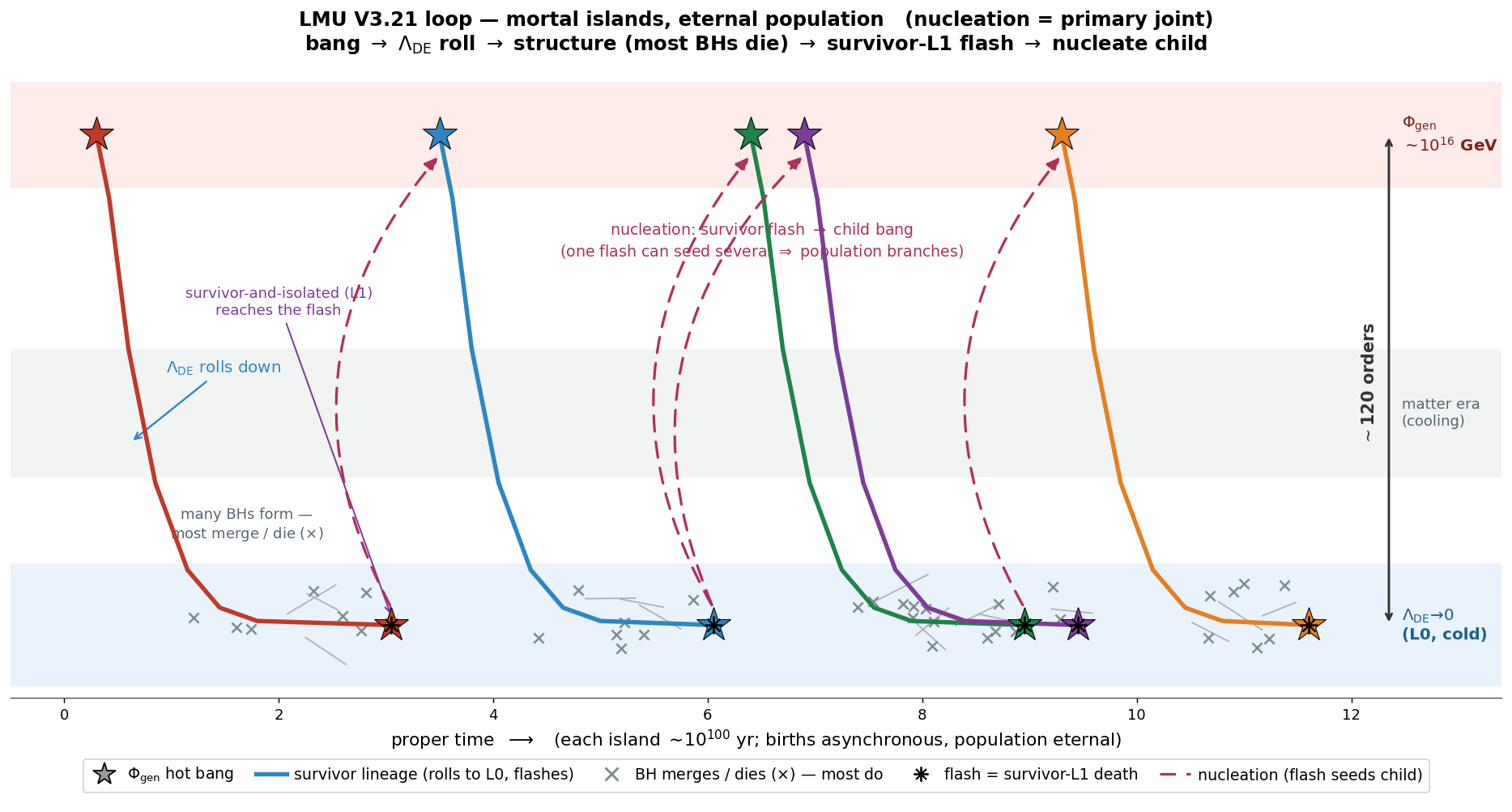
\includegraphics[width=0.99\textwidth]{lmu_v321_loop_cascade.png}
\caption{The loop as a cascade, on an energy axis (hot $\Phi_{\rm gen}$ at top, cold $\Lambda_{\rm DE}\!\to\!0$ at the floor). Each lineage is a hot bang, a roll down to the $L0$ floor (the $A$-field thawing toward zero), a long cold span in which most black holes merge or die ($\times$), and the survivor-and-isolated $L1$'s terminal flash --- which \emph{nucleates} one or more child bangs (B-primary; a flash can seed several). Births are asynchronous and the population is eternal; the right brace marks the $\sim$120 orders of magnitude the joint must bridge. \emph{Survival, not size}: of many holes, only the survivor in each island reaches the flash that seeds the next aeon. \design\ (the composition).}
\label{fig:loopcascade}
\end{figure}

% ---------------------------------------------------------------------
\section{B1$'$ --- the export ledger and the measured rate $g$}
\begin{equation}
S_{\rm out}^{(N)}=S_{\rm leftover}^{(N)}+\tfrac43\!\sum_{\text{all }i}S_{\rm BH}\bigl(M_i^{(N)}\bigr)=(1+g)\,S_{\rm fix},
\qquad g=\frac{(4/3)\,\Sigma S_{\rm BH}}{S_{\rm bath}}
\own{Zurek 1982; Tolman 1934}
\label{eq:b1export}
\end{equation}
$g$ is \emph{intensive and measured} --- an entropy-density ratio that island size cannot tune:
\begin{center}\small
\begin{tabular}{lll}\toprule
$g$ floor (only $M\,{\ge}\,10^9\,M_\odot$ holes, $n=10^{-5}\,$Mpc$^{-3}$) & $1.7\times10^{13}$ & BHMF only\\
$g$ fiducial (observable-universe budget) & $\mathbf{4.0\times10^{14}}$ & Egan--Lineweaver 2010\\
$g$ post-ladder (mass density in $10^{10\text{--}11}M_\odot$ survivors) & $2\times10^{16}$ (V3.7: $7.4\times10^{16}$) & $S\propto M^2$\\\bottomrule
\end{tabular}\end{center}
behind it: Soltan 1982; Marconi--Hunt 2004; Shankar, Weinberg \& Miralda-Escud\'e 2009. \Fact\ (R6 recomputation for this assembly: floor $1.65\times10^{13}$; fiducial $4.01\times10^{14}$, $\log_{10}=14.60$, from the Egan--Lineweaver $S_{\rm BH}$ budget $3.1\times10^{104}\,k_B$ over the observed bath $1.03\times10^{90}\,k_B$ per observable volume; the post-ladder figure is assumption-dependent --- it locks the Soltan-chain mass density into $10^{11}\,M_\odot$ holes --- and reproduces to order of magnitude.)

% ---------------------------------------------------------------------
\section{Why entropy is the invariant channel --- the conformal boundary and $z_{\rm aeon}$}
\noindent\Auditor\ \textbf{[B-alt: the conformal-rescale joint.]} This section and the $z_{\rm aeon}$ apparatus belong to the \emph{alternative} joint (B-alt; full $V_{\min}$/G1/G2 treatment in Part~VII). Under the primary joint (B-primary nucleation, above) there is no rescale: entropy is handled by ordinary $L0$ dilution plus a fresh per-pocket reheating, and $z_{\rm aeon}$ does not arise. The section is kept intact and valid as the alternative.
\noindent\emph{(Relocated from the archive's dark-energy module in V3.5: this is the justification of B1$'$ --- entropy is the cross-aeon bridge variable because the rescale cannot touch it.)}
The survivor's terminal flash is all-massless, and 3.4 keeps Penrose's conformal rescale \emph{scoped to that channel only} (massive debris persists in the reservoir L0; it never enters the boundary). The rescale is a Weyl map $\tilde g_{\mu\nu}=\Omega^2 g_{\mu\nu}$, and the open item $z_{\rm aeon}$ is the magnitude of that rescale --- the ``blueshift'' that gilds the cold evaporated end-state into a hot dense start.

\subsection{What the map fixes (the derivable part)}
Under $\tilde g=\Omega^2 g$, the transformation rules are standard: lengths and proper times scale as $\Omega$, energies and temperatures as $\Omega^{-1}$, a mass ruler as $\Omega^{-1}$ (the V1.5 ``$M\!\sim\!\Omega^{-1}$'' scaling, correct for this channel), while \emph{massless} field equations are invariant. The earlier ``$\mathcal M_\Omega$ carry operator'' that mapped mass, spin axis, and position across the boundary is therefore \textbf{superseded for massive content} in 3.4 --- such content rides the reservoir, not the rescale --- and survives only as the conformal map on the massless radiation. \Auditor

\subsection{Why the entropy route is blocked (the auditor result)}
The proposed first-principles derivation --- $z_{\rm aeon}$ from a critical-to-initial entropy ratio $S_{\rm crit}/S_{\rm initial}$ --- \textbf{cannot work}, for a reason internal to the construction. The boundary channel is, by design, the genuinely scale-free one; and the entropy of massless radiation is \emph{conformally invariant} (photon number is preserved under $g\!\to\!\Omega^2 g$ --- this is the very fact Penrose's cyclic cosmology rests on). The survivor of mass $M_\bullet$ evaporates with a radiation entropy ($4/3$ ratio from Zurek 1982)
\begin{equation}
S_{\rm rad}\simeq \tfrac{4}{3}\,S_{\rm BH}\simeq \tfrac{4}{3}\,(1.05\times10^{77})\,(M_\bullet/\msun)^2\ k_B
\ \approx\ 1.4\times10^{101}\,k_B\quad(M_\bullet\sim10^{12}\,\msun),
\end{equation}
matching the per-zone entropy scale (at the V3.5 canonical band top $10^{11}\,\msun$: $S_{\rm rad}=1.40\times10^{99}\,k_B$, the order of the per-island $S_{\rm fix}=2.8\times10^{99}\,k_B$ of Part~V; the $10^{12}$ figure shown is the upper illustration). Because this entropy is carried across the boundary unchanged, $S_{\rm initial}=S_{\rm rad}$: \textbf{the rescale generates no entropy ratio to fix $z_{\rm aeon}$ with.} What is left to set the scale is the gluing condition itself --- the temperature at which the cold evaporation (with $T_{\rm Hawking}\!\sim\!10^{-20}$~K for a $10^{12}\,\msun$ hole) is matched to a hot start (a ``blueshift'' $\sim T_{\rm hot}/T_{\rm cold}\!\sim\!10^{47}$) --- and that depends on the global structure beyond the causal horizon.

\textbf{Two consequences.}
\begin{itemize}[leftmargin=1.3em,itemsep=2pt]
\item \textbf{It explains the ambiguity.} The factor-$10^{20}$ uncertainty previously attached to the $S_{\rm crit}/S_{\rm initial}$ heuristic was not a precision that better work would sharpen; the ratio it relied on does not exist, because the relevant entropy is preserved, not reset.
\item \textbf{It validates 3.4's entropy stance.} If the conformal rescale cannot reset entropy (it preserves the massless entropy), then the population's ever-rising entropy must be handled some other way --- which is exactly 3.4's choice: \emph{diluted in the infinite reservoir, not reset}. The conformal-boundary audit and the closure choice agree.
\end{itemize}

\textbf{Verdict.} $z_{\rm aeon}$ is not a \emph{solvable} open item awaiting a derivation; it is an \emph{irreducible} one, set by a beyond-horizon gluing, in the same epistemic class as the Weyl-smoothness initial condition (O1) and the infinite-reservoir assumption (O3). The honest math-pass outcome is not a number but a boundary on knowledge: here is precisely why no number is derivable. \Open


% ---------------------------------------------------------------------
\section{B2$'$ --- sorting and partition}
Massless content crosses; every rest-mass lump goes one-way to $L0$ (re-entry only as the seed-flux channel). The corpse hosts $N_{\rm child}=f_{\rm part}(1+g)$ children, each rescaling a comoving patch holding exactly $S_{\rm fix}$; the un-nucleated remainder dilutes in $L0$ forever. Crossing is conformal \emph{per patch} (Penrose 2010; matching conditions Tod), a deliberate departure from CCC's global rescale; the explicit $x^\mu$ rule for lumps and patch boundaries is the committed-but-unwritten item \open{} (F2, blast radius: operator level). \design/\hyp\ \Auditor\ \textbf{[route note].} The conformal-per-patch crossing is the B-alt reading; under B-primary each child is an \emph{independent} nucleation event, so the partition \emph{count} $N_{\rm child}$ is route-agnostic while the crossing \emph{mechanism} is not.

% ---------------------------------------------------------------------
\section{B3$'$ --- per-round re-initialization}
$A\to A_i=2.70\,M_p$; $\eta$ at baryogenesis (the three conditions: Sakharov 1967); $P(k)$ amplitude and shape; spin axes $\hat n$ per the carry rules. All mechanisms \open{} --- this is where the framework's unexplained initial data lives, by design and said out loud.

% ---------------------------------------------------------------------
\section{B4$'$ --- minting}
\begin{equation}
N_\gamma=\frac{f_\gamma\,S_{\rm fix}}{3.60\,k_B},\qquad
M_b=\eta\,m_p\,N_\gamma,\qquad
M_{\rm DM}=\frac{\Omega_c}{\Omega_b}\,M_b=5.36\,M_b
\own{$\eta,\Omega$: Planck 2018 (BBN deuterium concordance, Cooke et al.\ 2018, independently fixes the same $\eta$); bookkeeping: Kolb--Turner}
\label{eq:b4mint}
\end{equation}
$\hookrightarrow$ recomputed constants (R6, fresh for this assembly): $f_\gamma=0.5116$, $s/n_\gamma=3.6016\,k_B$, $n_b=0.2504$\,m$^{-3}$, coherence $\rho_b/\Omega_b\rho_c=1.00$ (definition-level --- $\eta$ is measured as this ratio; recorded as internal consistency, not a test). DM is minted fresh each round as a collisionless thermal relic, symmetric with baryons (passes the Bullet Cluster). \textbf{The 5:1 ratio is matched, not predicted:} freeze-out gives $\Omega_{\rm DM}\propto1/\langle\sigma v\rangle$, and the canonical $\langle\sigma v\rangle\simeq3\times10^{-26}$\,cm$^3$\,s$^{-1}$ is the value \emph{chosen} to land it (Steigman et al.\ 2012). Direct-detection nulls (LZ 2024: $\sigma_{\rm SI}\lesssim\,$few$\,\times10^{-48}$\,cm$^2$ at tens of GeV; XENONnT) close the classic WIMP corridor, so the realization must live in still-open corridors (e.g.\ dark-sector freeze-out), with $N_{\rm eff}=2.99\pm0.17$ (Planck 2018) bounding light relics. The parent's mass reaches each child \emph{only as radiation}, re-minted here: the material lineage is $1\to\sim\!10^{14}$, not $1\to1$. \factth{} components, \hyp{} composition.

% ---------------------------------------------------------------------


\textbf{Anti-drift: an anomalously old star is not a previous-aeon relic.} Two facts and one architectural point close this off. \emph{(i) No star is \emph{robustly} older than the Universe.} Every candidate that appeared so sat within its error bar or was revised by better data and modelling: the ``Methuselah'' star HD~140283, once thought $\sim$16\,Gyr, was lowered by an improved \emph{HST} parallax to $14.46\pm0.8$\,Gyr (Bond et al.\ 2013, ApJL 765, L12 --- already consistent with $13.8$\,Gyr within its $\pm0.8$ error), and to $12\pm0.5$\,Gyr by Tang \& Joyce (2021, RNAAS 5, 117) with updated interferometric/Gaia parameters (Karovicova et al.\ 2020) and mixing-length calibration; a 2025 asteroseismic analysis (A\&A) returns $14.2\pm0.4$\,Gyr, again consistent with the cosmic age once systematics are folded in. The age is \emph{model-dependent}, and no estimate robustly exceeds the Universe --- the ``too old'' appearance is a modelling/parameter artefact, not a measurement. \emph{(ii) ``Older than the galaxy'' is a category error:} a galaxy's age is \emph{defined} by its oldest stars; the Milky Way's $\sim$13\,Gyr halo/old-disc stars \emph{are} its first generation, not something predating it. \emph{(iii) Architecture:} each aeon re-mints baryons and dark matter at its hot start (B4'); what persists across $L0$ is a \emph{black-hole-scale lump} with a genuine past, \emph{not} a star, and the child hot start reprocesses everything --- so stars form fresh each aeon. Therefore no stellar age can encode ``previous aeon.'' A claim that an unusually old star evidences a prior cycle would be a CCC-style overreach the ledger explicitly forbids: the loop's only carried datum is a BH seed (no age), through a hot start (clock-erasing). \Auditor\ (the inference) / \Fact\ (the stellar-age literature) / \Hyp\ (the $L0$ lump persistence). \emph{Sharpening (V3.16) --- the hot start is a universal eraser:} the child reheat reaches $T_{\rm hot}\sim6\times10^{27}$\,K, and even the BBN epoch at $\sim10^{9}$\,K leaves no complex nuclei; at these temperatures there are no atoms, no nuclei, not even nucleons, so \emph{no} macroscopic object --- star, white dwarf, rock --- can survive a hot start, in LMU or in any hot-bounce cyclic model (CCC, ekpyrotic). Only massless radiation crosses the conformal boundary and only a BH-scale lump (no readable age) persists in $L0$; a putative previous-aeon relic one could \emph{date} is therefore excluded by thermodynamics, not merely unobserved. \Fact\ / \Auditor

\section{Endowment gathering --- no unique parent (the surviving S7 addendum)}
When a new zone forms in $L0$ it gathers from whatever dead-loop outputs lie in its region:
\[
S_{\rm endow}=\sum_k w_k\,S_{{\rm out},k}\qquad(\text{gathering weights }w_k\ \text{over reachable dead loops}),
\]
so the $1{:}1$ parent$\to$child lineage of earlier drafts was too strict, in two ways. \textbf{(i) No unique parent:} the lump channel is likewise generic, not exotic --- new zones form from \emph{mixed} $L0$ debris fields, so carry-through seeds need no special neighbour geometry (the explicit $x^\mu$ rule remains item F2, \open). \textbf{(ii) $M_{L1}$ responds to endowment --- slowly:} the survivor is the \emph{maximum} of the merger-tree tail, so extreme-value scaling applies; with the exponential cluster tail folded through the \emph{cluster-end owned} slopes $M_\bullet\propto M_{\rm halo}^{\beta}$, $\beta\approx1.05$--$1.35$ (Bogd\'an et al.\ 2018, observed; Bassini et al.\ 2019, simulations --- item E resolved; the old $\beta\approx0.7$ was an orphan matching the \emph{stellar} BCG--halo slope), $d\log_{10}M_{L1}\approx0.15$--$0.27$ dex per decade of endowment. Gathering $10\times$ more dead loops moves the survivor only $\times1.4$--$1.9$; gathering half, $-0.05$ to $-0.08$ dex. The fixed point of earlier drafts is therefore a \textbf{fixed band with a multiplicative walk}: unbiased gathering keeps $\log M_{L1}$ within $\pm0.7$--$1.2$ dex of $11$ over $50$ rounds. The drifted branch that stacked a gathering$\,\propto\,$L0-growth link on top (and its round count to a ceiling) is \textbf{retired} --- the link is unestablished (R2: cross-round extrapolation from zero measured rounds) and its ceiling premise died with the constant-$\Lambda$ interlude (Part~V, retired table). \Hyp\ (the band and EV scaling) / \Dead\ (the drift branch). \textbf{V3.7 stability audit:} the deterministic return map is \emph{flat} --- the next round's $M_{L1}$ is set by gathering statistics, not the parent's mass; slope $\lambda=\beta_{\rm eff}\cdot2\cdot(\text{survivor share of island export})\approx1.3\times10^{-15}$, so the band is \emph{restoring}. The $\pm0.7$--$1.2$ dex/50-round walk is the pessimistic random-walk-endowment envelope: Monte Carlo ($2\times10^4$ walkers) finds the floor unreachable in 50 rounds in every model, with median first passage $902$--$1714$ rounds under the document's own RW pessimism and never under i.i.d.\ gathering. \Auditor

\clearpage

% ===================== PART V =====================
\part{Results of the composed system}
\setcounter{section}{0}\setcounter{equation}{0}\setcounter{figure}{0}

% ---------------------------------------------------------------------
\section{Per-island fixed band}
\begin{center}\small
\begin{tabular}{ll}\toprule
$S_{\rm fix}$ & $2.80\times10^{99}\,k_B$ --- exact fixed point under equal partition\\
$V$ (today-equivalent) & $9.69\times10^{89}$\,m$^3$\\
$M_b$;\ $M_{\rm DM}$ & $2.04\times10^{32}$;\ $1.09\times10^{33}\,M_\odot$\\
$M_{L1}$ & $10^{10}$--$10^{11}\,M_\odot$ \textbf{band}, extreme-value scaling $\approx0.15$--$0.27$ dex per decade of endowment (owned $\beta$)\\
\bottomrule\end{tabular}\end{center}
The band slope follows Gumbel/extreme-value statistics (Fisher--Tippett 1928; Gnedenko 1943) for an exponential cluster tail with $M_{\max}\approx5$--$7\,M_*$, folded through $M_\bullet\propto M_{\rm halo}^{\beta}$ with the \textbf{cluster-end owned slopes} $\beta\approx1.05$ (Bogd\'an et al.\ 2018, observed, via the Lovisari et al.\ 2015 $kT$--$M_{500}$ chain) to $1.35\pm0.15$ (Bassini et al.\ 2019, simulations), giving $\approx0.15$--$0.27$ dex per decade of endowment (up to $0.33$ under galaxy-end slopes: Bandara et al.\ 2009; Ferrarese 2002; Li et al.\ 2024 weak lensing). The previously quoted $0.14$ used an unowned $\beta\approx0.7$ --- numerically coincident with the range's lower edge, but $0.7$ matches the \emph{stellar} $M_{*,\rm BCG}$--$M_{500}$ slope (Kravtsov et al.\ 2018; Bassini et al.\ 2019), not the black-hole one; the derivation is corrected and the orphan retired (item E, resolved 2026-06-10). Two knobs stay explicit: steeper Press--Schechter-type tails push the slope \emph{down}; the owned $\beta$ range pushes it \emph{up} from the old headline. Aggregation statistics drive any walk of the band (Part~IV \S6; $\pm0.7$--$1.2$ dex over 50 rounds); the old fork-5--linked drift is retired (\S4). \hyp\ \textbf{V3.7 floor:} the band has a computed lower boundary --- $R_{\rm isl}(M)\propto M^{2/3}$ meets $\lambda_J$ at $M_{\rm floor}\approx6.4\times10^{5}\,\msun$, $\approx5.19$ dex below the band centre ($10^{11}\,\msun$) (below it island modes fall sub-Jeans and the open hierarchy stalls) --- and no operative ceiling ($M_{\rm Nariai}\to\infty$ on the dust interlude; the live ceiling sits $+11.3$ dex away from the $10^{11}\,M_\odot$ band top). \Auditor\ \textbf{Nariai clarification (V3.15).} The divergence is not a loophole but a reading of the same SdS condition: $M_{\rm Nariai}=c^3/(3\sqrt3\,GH)$ is fixed by the \emph{phase's} $H$, not a universal constant, and at $L0$ the field has relaxed to $A\approx0\Rightarrow\Lambda=0\Rightarrow H\to0$, so the ceiling is evaluated on the reservoir's vanishing Hubble rate, not the present epoch's $H_0$ --- hence it diverges as geometry (the degenerate horizon recedes), not as an artefact. But ``no Nariai ceiling'' must not be misread as $M_{L1}\to\infty$: the bound that actually operates on the survivor is the extreme-value (Gumbel) law above --- the survivor is the maximum of $\sim\!N$ merger-tree draws, and the maximum of an exponential tail grows as $M_*\ln N$, \emph{logarithmically}, so even at $N\sim10^{78}$ ($\ln N\approx180$) it stays within $\sim$2 dex of the characteristic cluster scale, landing in the $10^{10}$--$10^{11}\,\msun$ band already quoted, never at infinity. The accretion ceiling $\sim5\times10^{10}\,\msun$ (King 2016; Inayoshi--Haiman 2016) caps growth-by-\emph{accretion} but not growth-by-merger, so it does not bound the survivor either. One honest caveat: were the cluster tail a \emph{power law} (Fr\'echet domain) rather than exponential, the maximum would grow as $N^{1/\alpha}$ (super-logarithmic) and the band would cease to be self-capping --- so the logarithmic band is conditional on a Schechter (exponentially-cut) tail, and the tail-slope carries the same \hyp\ standing as the band slope above. \Auditor

This island-volume scale is also a \textbf{lower bound on island size}: the measured entropy density of the bath plus the $S_{\rm BH}$ of a band-top L1 survivor require $V\ge1.36\times10^{9}$ observable volumes ($R\ge1107\,R_{\rm obs}$, computed from the survivor's radiation entropy $S_{\rm rad}=\tfrac{4}{3}S_{\rm BH}$ alone; this assembly's R6 run, which uses the island's full $S_{\rm fix}$, gives $V/V_{\rm obs}=2.7\times10^{9}$, $R=1395\,R_{\rm obs}$ --- above the bound by exactly $S_{\rm fix}/S_{\rm rad}=2.0$: a bound plus a consistency check, not the same statement twice). \Fact\ (the arithmetic) / \design\ (the reading) \textbf{L1-start as a self-location (V3.15).} The same island bound carries an anthropic corollary, recorded as an interpretive consistency, not a result. Our observable patch is $\le(1107)^{-3}\approx7\times10^{-10}$ of an island ($R\ge1107\,R_{\rm obs}$), and we sit \emph{after} the $L4\to L1$ ladder has populated --- the epoch in which galaxies, stars, and observers exist. A self-locating observer expects exactly this conjunction: structure-bound observers find themselves in a small sub-patch of a much larger island and in the structure-forming era, never at the bare $L1$ start nor in the empty pre-ladder reservoir (the Carter 1974 selection principle; cf.\ the perfect-cosmological-principle echo applied only at $L0$, Part~V \S2). So our unremarkable position is what the selection effect predicts and adds \emph{no} falsifier; it must not be read as predicting the epoch --- the why-now cost stays booked in the field mass $m$ (Part~II), not re-credited here. \Auditor\ / \design

% ---------------------------------------------------------------------
\section{The two-sector verdict and the Tolman ledger}
\begin{equation}
S_{\rm tot}^{(n)}=(1+g)^n\,S_{\rm tot}^{(0)}\qquad\text{(monotone; the second law as a rate equation)}
\own{Tolman 1934}
\end{equation}
with $g$ the \emph{measured} rate of Part~IV \S1 (floor $1.7\times10^{13}$; fiducial $4.0\times10^{14}$; post-ladder $\sim\!2\times10^{16}$, V3.7 recompute $7.4\times10^{16}$ --- reproduced here because this is the ledger that pays it).
\begin{center}
\fbox{\parbox{0.9\textwidth}{\centering
\textbf{Fork-5 condition (background-independent counting):} the population must colonize fresh comoving extent at $\ge(1+g)\approx10^{14.6}$ per generation, forever $\iff$ \textbf{L0 unbounded}. Kill: any finite L0, or sub-exponential capacity.}}
\end{center}
Per island the loop closes in matter --- densities, the ladder, the BHMF, and the $M_{L1}$ band repeat --- and ratchets in \emph{extent} (Fig.~\ref{fig:ledger}). The entropy resolution is by dilution into expanding space (Steinhardt--Turok 2002) plus jettison outside the recycling patch (Baum--Frampton 2007), with a steady mortal-islands/eternal-population structure (Aguirre--Gratton 2002; population bookkeeping Garriga--Vilenkin; structural echo of the perfect cosmological principle, Bondi--Gold--Hoyle 1948, applied only at the unobservable L0 level). The dilution lane's newest realization: Itzhaki, Peleg \& Steinhardt 2026 (JCAP 05, 084; arXiv:2508.09745) --- a complete cyclic bouncing cosmology from string-theory components, under perturbative control throughout; nearest-neighbour competitor to fork 5 alongside CCC, to be read against the Kinney 2026 re-kill of IS-cyclic carried in the borrowed-legs audit (V3.8) --- whether that argument reaches the string construction is unchecked. \Auditor Eckstein 2023 dissolves the Tolman growth at the definition level via entanglement entropy of a global pure state; LMU keeps the counting version and carries Eckstein as the literature alternative. L0 is \emph{closed in state space per island, an irreversible branching tree globally} --- ``closed circuit'' in the first sense only. \hyp{} riding fork 5.

\begin{figure}[h]\centering
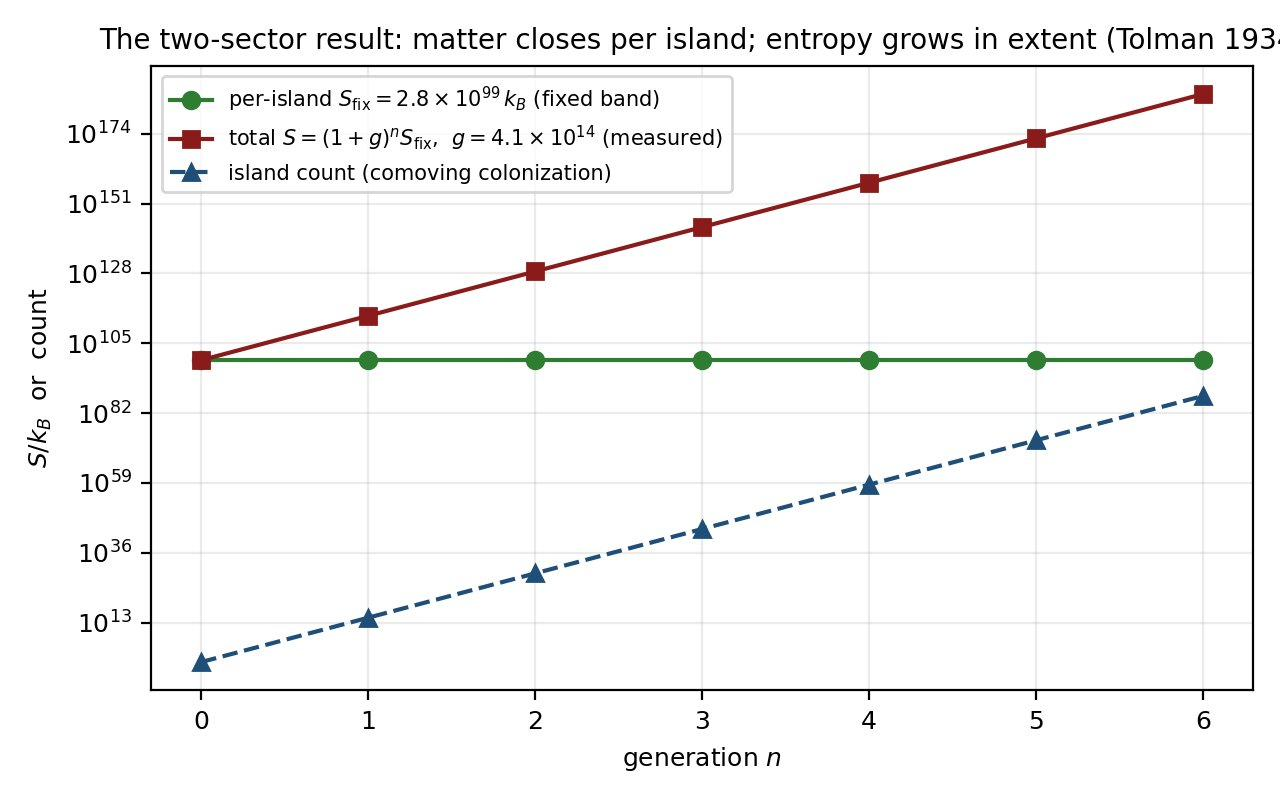
\includegraphics[width=0.78\textwidth]{fig4_ledger.png}
\caption{Per-island quantities are flat (fixed band); total entropy and island count grow geometrically with the \emph{measured} $g$. The whole Tolman load sits on fork 5.}
\label{fig:ledger}
\end{figure}

% ---------------------------------------------------------------------
\section{Predictions and standing tensions}
\textbf{Carry-through predictions:} relic spin-axis alignment, testable by NewAthena and LISA (late 2030s); ``too-early'' lump-seeded holes in young zones (the seed-flux channel). \hyp

\textbf{Standing tension --- mandatory flag (travels with every reuse of the ladder):} the cluster spin-down expectation ($a_\star\sim0.55$) is in tension with the M87 spin $a_\star\gtrsim0.8$ reported from EHT Doppler beaming (Drew et al.\ 2025, ApJL 984 L31, a lower limit; contested by Wong et al.\ 2025 polarimetry) --- status \open\ (contested), not falsified; the relic-side spin decoupling is unmeasurable in principle (Part~VI \S21). \textbf{V3.7 inversion:} the spin walk $a=a_0/\sqrt{1+N}$ (Hughes \& Blandford 2003) turns $a_\star\ge0.8$ into $N_{\rm misaligned}\le0.56$--$2.26$ (lower: pure walk from $a_0=0.998$; upper: walk allowing accretion re-spin, lift $\times1.45$) against the modeled $5.9$ --- tension factor $2.6$--$10.6$, i.e.\ an aligned-merger fraction $\ge62\%$ where the model assumed isotropy. \hyp\ / \Auditor\ Watch for new measurements (ngEHT/BHEX, $\sim$2030s).

% ---------------------------------------------------------------------
\section{Retired numbers (V3.5) --- nothing on this list may be cited as live}
Each entry names the superseded figure, why it died, and the live replacement. Any later document citing one of these as current is in error.
\begin{center}\small
\begin{tabular}{@{}p{0.34\textwidth}p{0.30\textwidth}p{0.30\textwidth}@{}}\toprule
\textbf{Retired item} & \textbf{Why retired} & \textbf{Live replacement}\\\midrule
$g\in(0,10]$ and the $\times2$/round kill bound & survivor-class truncation understated $g$ by $\sim$14 orders & measured $g$: floor $1.7\times10^{13}$, fiducial $4.0\times10^{14}$ (Part~IV \S1)\\
``$\approx267$ rounds to Nariai'' (band drift to a ceiling) & both premises dead: the $\times2$/round link is unestablished (R2) and the constant-$\Lambda$ ceiling does not operate on the dust interlude & none; band walk per Part~IV \S6 ($M_{\rm Nariai}\to\infty$ as $H\to0$)\\
Constant-$\Lambda$ interlude package: e-folds $10^{90}$; de Sitter horizon $1.65\times10^{26}$\,m; $s_{L0}=2.5\times10^{-67}\,k_B\,$m$^{-3}$; the $0.17\,M_\odot$ \emph{transport verdict} & Correction~1: the interlude is a dust era, not de Sitter (the A-field has $V_{\min}=0$, $H\to0$) & dust-era kinematics $a\propto t^{2/3}$, $H=2/(3t)$; the timing race (Part~III \S2)\\
Nariai $1.8\times10^{22}\,M_\odot$ as a \emph{universal} ceiling & the ceiling is a live-phase (acceleration-window) statement only & scoped ceiling, Part~III \S1 (eq.\ Nariai); $M_{\rm Nariai}\to\infty$ on the interlude\\
``Encounter rate $\to0$'' / cross-island terms default-negligible & de Sitter artifact (no event horizon on the dust era) & cross-island forced fork $=$ the main interlude channel (Part~III \S2); F5 closed by retirement --- no successor will be derived (Part~VII, G)\\
``Survivor isolated forever'' & isolation holds only during the transient acceleration window, $a\approx0.6\to$ few--20 & scoped isolation clause (Part~I; Part~III \S2); survival-based L1 definition unchanged\\
NGC~1277 mass $1.7\times10^{10}\,M_\odot$ (van den Bosch et al.\ 2012) & superseded by the adaptive-optics dynamical mass & Walsh et al.\ 2016: $(4.9\pm1.6)\times10^{9}\,M_\odot$; extreme-overmass flagship: TON~618\\\bottomrule
\end{tabular}\end{center}
\emph{Scope notes for the grep-audit:} the $10^{90}$\,\emph{yr} duration of the L1 endgame (Part~VI \S10) and the $w_a$ value $-0.17$ (Part~II) are different quantities that happen to share digits with retired items; they are live. \Auditor

% ---------------------------------------------------------------------
\section{R6 recomputation record (this assembly)}
All Part IV--V numbers were recomputed fresh for the V3.5 pass, none inherited, and carry into V3.6 unchanged (the V3.6 ledger pass adds the item-F gate and corrected-band numbers, each R6-recomputed in its session record): $S_{\rm BH}(10^{11}M_\odot)=1.049\times10^{99}\,k_B$ (coefficient $1.049\times10^{77}$); $\tau_{\rm evap}(10^{11})=2.10\times10^{100}$\,yr, $(10^{12})=2.10\times10^{103}$\,yr; $M_{\rm Nariai}(H_0{=}67.4)=1.789\times10^{22}\,M_\odot$; $f_\gamma=0.5116$; $s_\gamma/n_\gamma=3.6016\,k_B$; $n_b=0.2504$\,m$^{-3}$; $g_{\rm floor}=1.65\times10^{13}$, $g_{\rm fid}=4.01\times10^{14}$ ($\log_{10}=14.60$); $S_{\rm fix}=s_{\rm bath}V=2.800\times10^{99}\,k_B$; $M_b=2.040\times10^{32}\,M_\odot$; $M_{\rm DM}=1.094\times10^{33}\,M_\odot$; Gunn--Gott race $\tau_{\rm evap}/t_{\rm coll}(\delta_i{=}1)\sim10^{89\text{--}90}$, $(\delta_i{=}10^{-3})\sim10^{85}$; $p(f{=}1/64)=0.043$, growth $\times4\times10^{2}$; KG $m{=}0.8$: $(w_0,w_a)=(-0.9080,-0.1438)$; NGC~384 $\Delta M_\sigma=+0.296$; relic six $+0.227\pm0.099$. \Fact\ (this run)

\clearpage

\part{Verification and empirical confrontation}
\setcounter{section}{0}\setcounter{equation}{0}\setcounter{figure}{0}

\noindent\textbf{What this part adds.} Parts I--III state the framework's equations and results; this part records an independent re-derivation of them and then confronts the one genuinely distinctive, falsifiable prediction --- the relic spin --- with real measured data. The honest outcome, stated up front: every number reproduces, the ladder runs as a single forward map that sorts real galaxies by eating-position, and the spin decoupling is the mass-robust core that survives every stress test --- yet that same decoupling is, for every object where it would discriminate, currently \emph{unmeasurable}. The framework's sharpest claim is therefore correctly \Open, neither confirmed nor dead. \Auditor

\noindent\textbf{Update (2026-07, adjudicated).} A later audit pass sharpened the status of the one distinctive claim (the relic/cluster spin decoupling); the two findings live in the \S5 rows and the [Open] status line below: (i) the relic side is \emph{unmeasurable in principle} --- a relic's defining quiescence disables every spin probe (X-ray reflection, shadow illumination, merger-GW), so only a still-accreting relic is reachable; and (ii) M87$^*$ spin measurements currently disagree by method --- Doppler-beaming of the EHT bright spot gives $a_*\gtrsim0.8$ (Drew et al.\ 2025, ApJL 984 L31, quoted as a lower limit), while polarimetric analysis disfavours high spin (Wong et al.\ 2025). Status stays \open\ (contested); the method-level disagreement itself sharpens F2's value as a discriminator in the BHEX era. \Auditor

\section{Independent verification of the analytic and ODE sectors}
Every closed-form number in Parts I--III was recomputed from fundamental constants alone; all reproduce to rounding --- Hawking $T_H,L,\tau_{\rm evap}$; $M_{\rm Nariai}=1.79\times10^{22}\,\msun$ at $H_0=67.4$; $S_{\rm BH}=1.05\times10^{77}(M/\msun)^2 k_B$; $S_{\rm rad}=\tfrac43 S_{\rm BH}=1.4\times10^{101}\,k_B$ at $10^{12}\,\msun$ (upper illustration; $1.40\times10^{99}\,k_B$ at the band top $10^{11}\,\msun$); the clustering threshold $\pi^2/4=2.47$; the Eddington seed-growth times. Both ODE sectors re-integrate to the same answers: the Klein--Gordon field reaches $w_0\!\approx\!-0.89$ at its DESI-closest displacement and never crosses $w=-1$, and the matter-ladder spin decoupling reproduces (\S3). The two analytic corrections folded into Part~III --- the Nariai coefficient $1/3\sqrt3$ and the Zurek $4/3$ entropy ratio --- are confirmed. \Fact

\section{The ladder as a single forward map}
\begin{figure}[h]
\centering
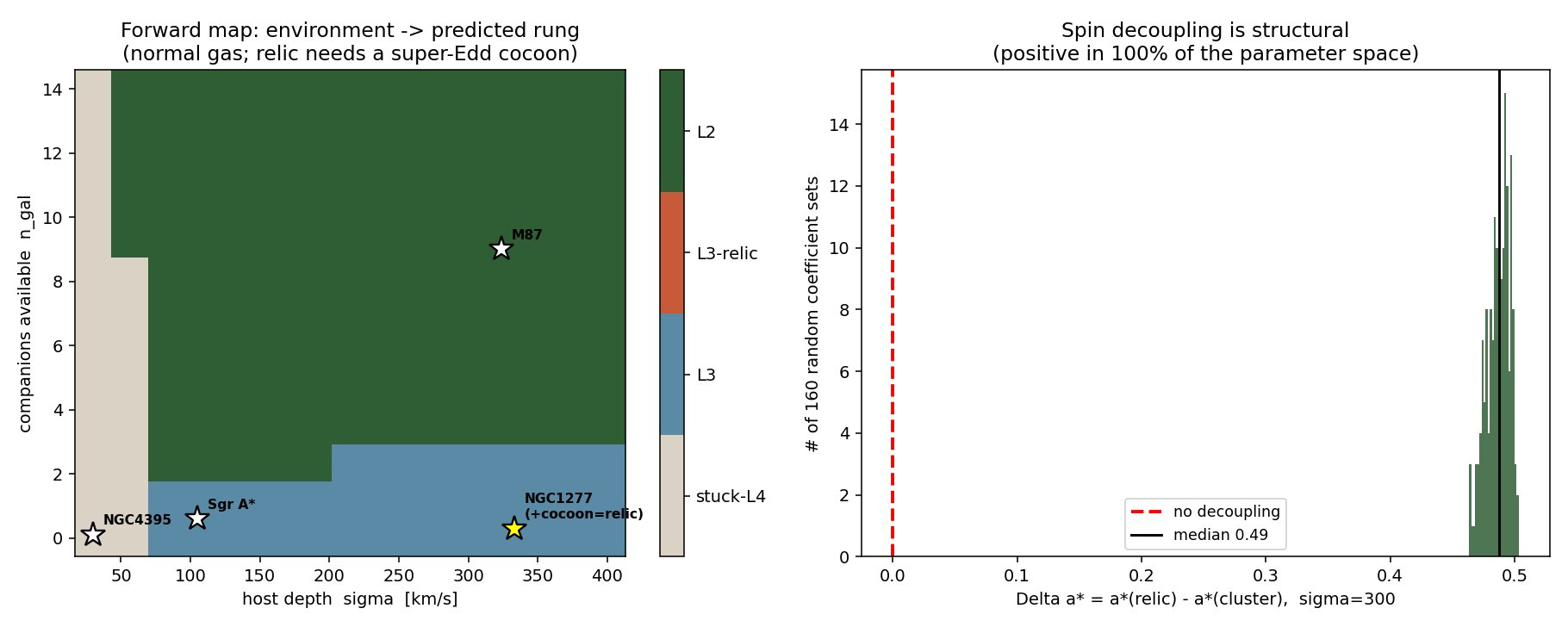
\includegraphics[width=\textwidth]{ladder_forward_map.png}
\caption{\textbf{Left:} run as one system across the environment plane, the five equations partition $(\sigma,n_{\rm gal})$ into the four rungs; four real galaxies (one per class) land in their observed bins. \textbf{Right:} the spin decoupling $\Delta a_\ast=a_\ast^{\rm relic}-a_\ast^{\rm cluster}$ is positive in 100\% of a 160-draw coefficient sweep (median 0.49).}
\end{figure}
Across the environment plane the five equations partition $(\sigma,n_{\rm gal})$ into the four rungs (Fig.~1, left): shallow hosts $\to$ stuck-L4, deep-and-companion-rich $\to$ L2, deep-and-isolated-with-a-cocoon $\to$ L3-relic, the rest $\to$ L3. Four real galaxies, one per class, fall in their observed bins --- Sgr~A* (L3), M87 (L2), NGC~1277 (L3-relic), NGC~4395 (stuck-L4). \textbf{The decisive demonstration is M87 vs NGC~1277:} near-identical dispersion ($\sigma\!\approx\!324$ vs $317$, the adopted value of \S5) sorted into \emph{different} rungs by companions and gas history, not mass --- ``ranking by eating-position, not size,'' shown on two real objects. \textbf{This is a consistency classifier, not predictive validation:} the class is set by inputs ($n_{\rm gal}$, gas) that are read in, the sample is one object per class, and (Part~I) nothing here discriminates the framework from $\Lambda$CDM. \Design\ (the ranking) / \Auditor\ (the classifier and check).

\section{Mass--spin separability --- the decoupling is mass-robust}
A natural worry: the framework keys off spin, spin co-evolves with mass, so if the black-hole \emph{mass} is wrong the spin and rung are wrong too --- the equations would carry incomplete variables. This does not hold, for a structural reason. The spin equation of Part~I depends on $\dot M^{\rm acc}/M$ and $\Gamma_{\rm mrg}$, both invariant under a rescaling of the mass \emph{scale} (accretion and merger rates are each $\propto M$). Re-integrating the relic and cluster archetypes with the seed scaled by $\times0.1,\times1,\times10$ leaves the decoupling intact:
\begin{center}\small
\begin{tabular}{@{}lccc@{}}
\toprule
seed scale & relic $a_\ast$ & cluster $a_\ast$ & $\Delta a_\ast$ \\
\midrule
$\times0.1$ & 0.998 & 0.549 & $+0.45$ \\
$\times1$   & 0.998 & 0.522 & $+0.48$ \\
$\times10$  & 0.998 & 0.493 & $+0.51$ \\
\bottomrule
\end{tabular}
\end{center}
and a $\pm0.2$-dex shift in $M_\sigma$ moves the regulated spin by $<0.01$. The decoupling's \emph{sign and size} are set by the merger term's presence, not the mass scale; the absolute spin values carry the mass calibration, the falsifiable signature does not. \textbf{Choosing spin (not mass) as the axis is the correct response to exactly this worry.} \Auditor

\section{The spin-direction model --- magnitude robust, axis fragile}
\begin{figure}[h]
\centering
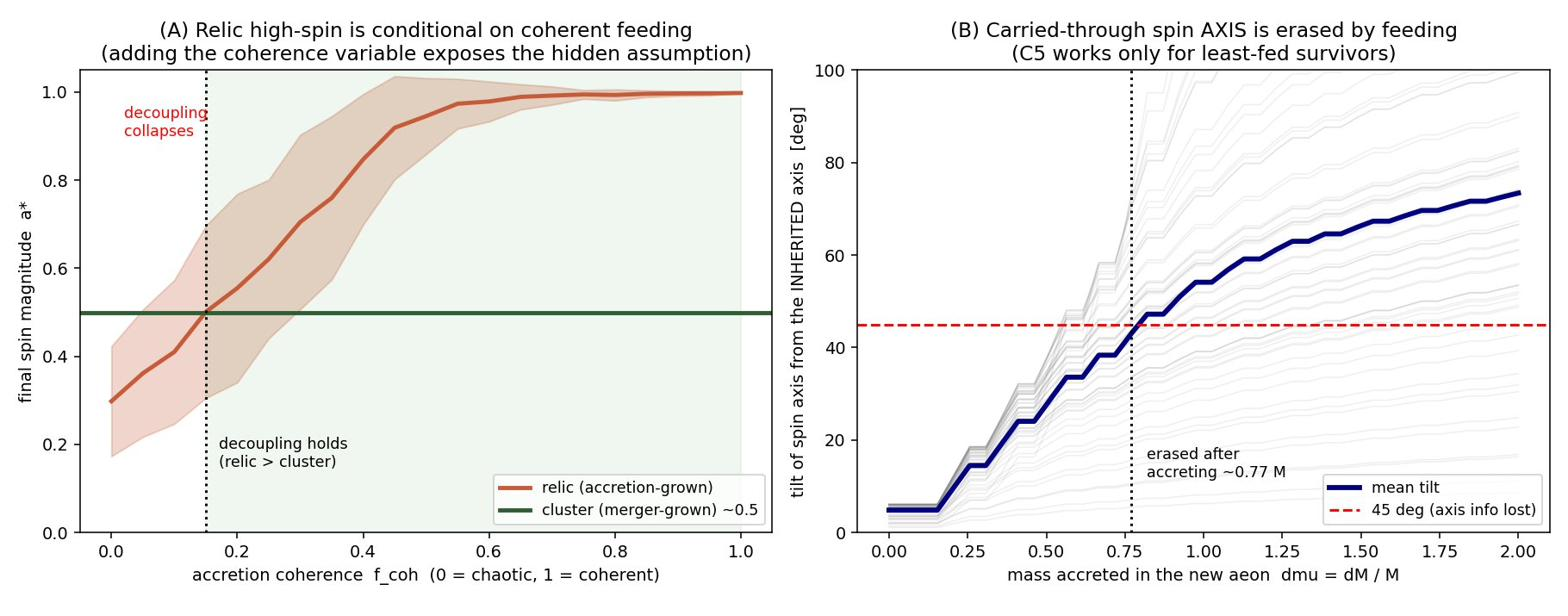
\includegraphics[width=\textwidth]{spin_axis_model.png}
\caption{\textbf{(A)} The magnitude decoupling survives once spin is a vector, but ``relic spins high'' is now explicitly conditional on coherent cocoon feeding ($f_{\rm coh}\!\gtrsim\!0.15$). \textbf{(B)} An inherited spin axis is tilted past $45^\circ$ after the survivor accretes $\sim$0.77 of its mass in the new aeon --- the carry-through axis is a selection-limited falsifier.}
\end{figure}
Promoting spin to a vector (magnitude $+$ axis), grounded in chaotic-versus-coherent accretion (King \& Pringle 2006), the spin-up budget (Bardeen 1970), and disk alignment (Bardeen--Petterson 1975): \textbf{(A)} the magnitude decoupling survives, now with its hidden assumption exposed --- ``relic spins high'' holds provided the cocoon accretion is coherent ($f_{\rm coh}\!\gtrsim\!0.15$, a mild condition for a single gas reservoir; Fig.~2A). \textbf{(B)} an \emph{inherited} spin axis is erased, tilted past $45^\circ$ once the survivor accretes $\sim$0.77 of its mass in the new aeon (Fig.~2B), so the carry-through axis prediction (C5) is a \emph{selection-limited} falsifier, alive only for the least-fed survivors. The variable \emph{refines, does not expand} the predictions; the robust content stays the spin-\emph{magnitude} decoupling. Coefficients are illustrative (the qualitative behaviour is the literature's; the exact numbers are not). \Hyp

\section{Confronting the distinctive prediction with data}
The framework's one distinctive, falsifiable claim: over-massive \emph{isolated} relics spin \emph{high} (accretion-built, bucking the general high-mass$\to$low-spin trend), while merger-built cluster BCGs spin \emph{low}. Confronted with real measurements:

\textbf{The measured-spin trend} (X-ray reflection sample, $\sim$50 holes; Reynolds 2013/2021 and the 2025 compilation) does show high spin at low mass and lower spin at high mass, attributed to accretion versus mergers \Fact\ --- \emph{consistent} with the decoupling, but this is the \emph{standard} interpretation (cosmological simulations predict the same), and the sample is too heterogeneous and selection-biased (X-ray reflection needs active accretion) to discriminate. \textbf{Consistent, non-discriminating.}

\textbf{The relics themselves are unmeasurable.} NGC~1277 and Mrk~1216 are quiescent --- no accretion, hence no X-ray reflection, no Fe~K$\alpha$, \emph{no spin}. The distinctive test cannot be run. Their \emph{masses} are well measured: for NGC~1277 the high-resolution adaptive-optics dynamical value is $M_\bullet=4.9\times10^{9}\,\msun$ ($\log M_\bullet=9.69\pm0.14$; Walsh et al.\ 2016, confirmed by Krajnovi\'c et al.\ 2018), revising down the original low-resolution van den Bosch et al.\ (2012) value (now retired; Part~V \S4); intermediate optical values run $\log M_\bullet\!\approx\!9.1$ (Graham et al.\ 2016) to $10.1$ (Y\i ld\i r\i m et al.\ 2015). At the adopted $\sigma=317\,\mathrm{km\,s^{-1}}$ the Walsh mass sits $\mathbf{+0.24}$~\textbf{dex above} the McConnell--Ma $M$--$\sigma$ relation --- consistent with the relic $+0.22\pm0.09$~dex offset (NGC~1277 is one of the $n=6$ calibrators). \emph{The framework's calibration should use the Walsh $9.69$, not the higher Y\i ld\i r\i m $10.1$; the dispersion of literature values ($\sim$1.1~dex) is itself a caution.} \Fact\ / \Auditor

\textbf{M87 is the one near-term test, and its spin is unconstrained.} As the canonical L2 the framework predicts a moderate-to-low spin ($a_\ast\!\sim\!0.5$). Published M87* spin estimates span $a_\ast\!\approx\!0.1$--$0.98$ and are strongly model-dependent: EHT imaging does not pin it; jet-power / Blandford--Znajek and Doppler-beaming methods lean moderate-to-high ($\sim$0.5--0.9, one 2025 method giving $\sim$0.8 as a lower limit), while a jet-boundary-shape method gives low ($\sim$0.2--0.3); and a 2025 EHT-polarimetry analysis \emph{disfavours high spin} for M87* (Wong et al.\ 2025, arXiv:2509.22639), pulling toward the moderate-to-low side. A Doppler-beaming analysis of the EHT bright spot pulls the other way: $a_*\gtrsim0.8$, quoted as a lower limit (Drew et al.\ 2025, ApJL 984 L31). The framework's $\sim$0.5 sits in the middle of that range --- \emph{consistent with everything, discriminating nothing}; only a confirmed near-maximal spin ($a_\ast\!\gtrsim\!0.9$) would tension the merger-spin-down picture. \Open

\textbf{Verdict.} The distinctive spin signature is structurally robust --- mass-invariant (\S3), surviving the coefficient sweep and the coherence/axis refinement (\S4) --- yet \emph{empirically blocked for every object where it would discriminate}: the relics are quiescent (no spin) and M87's spin spans the whole allowed range (no constraint). The framework bets against the observed high-mass$\to$low-spin trend for its key objects, with no data able to settle it. Correct status: \Open, neither confirmed nor dead. Unlock routes: NewAthena ($\sim$2037, any weakly-accreting relic), LISA (merger-remnant spins), ngEHT (M87 via polarimetry). \Auditor

\section{Attribution --- verification and empirical confrontation}
\begin{center}\small
\begin{tabular}{@{}p{0.45\textwidth}p{0.49\textwidth}@{}}
\toprule
Element & Owner / source \\
\midrule
Eating-position ranking; relic-spin falsifier; spin-as-axis choice & Pitarn (\Design) \\
Forward-map classifier; real-galaxy check; mass--spin separability tests; vector-spin model & editor pass (\Auditor) \\
Chaotic/coherent accretion; spin budget; disk alignment & King \& Pringle (2006); Bardeen (1970); Bardeen \& Petterson (1975) \\
Measured SMBH spins & Reynolds (2013, 2021) and 2025 compilation \\
NGC~1277 black-hole mass & Walsh et al.\ (2016); Krajnovi\'c et al.\ (2018); cf.\ van den Bosch et al.\ (2012), Y\i ld\i r\i m et al.\ (2015), Graham et al.\ (2016) \\
M87* spin estimates & EHT Collaboration; Feng \& Wu (2017); Nokhrina et al.\ (2019); Wong et al.\ (2025, arXiv:2509.22639, polarimetry --- disfavours high spin); Drew et al.\ (2025, ApJL 984 L31, Doppler beaming --- $a_*\gtrsim0.8$, lower limit); and others (model-dependent) \\
\bottomrule
\end{tabular}
\end{center}

\vspace{4pt}\hrule\vspace{4pt}
{\small Part~IV is the verification-and-confrontation half of the math pass. The analytic and ODE sectors reproduce independently; the ladder sorts four real galaxies by eating-position (a consistency classifier, not a discriminator); the spin decoupling is shown mass-robust (the correct answer to ``mass wrong $\Rightarrow$ all wrong'') and survives a vector-spin refinement that exposes its one condition (coherent feeding) and limits the carry-through axis to least-fed survivors. Confronted with data, the distinctive relic-spin claim is consistent-but-non-discriminating where spins exist, and unmeasurable for the relics themselves (quiescent) and unconstrained for M87 ($a_\ast$ spans 0.1--0.98). Correctly \Open --- the sharpest empirical claim is blocked by the physics of the measurement, not by being wrong.}

\vspace{10pt}\hrule\vspace{2pt}
\begin{center}{\LARGE\bfseries Part V --- Out-of-sample confrontation \& 2026 audit update}\end{center}
\vspace{1pt}\hrule\vspace{5pt}
{\small Part~IV tested the spin claim and the ladder-as-classifier. Part~V folds in the 2026 confrontation that was not yet included: a genuine \emph{out-of-sample} relic ($\Mbh$ measured directly, outside the calibration set), the mass-free merger diagnostic, the dwarf empty-centre axes, and the structural reason the distinctive content is either mainstream or measurement-blocked. New owners named; \Auditor\ marks an audit step.}

\section{The relic over-massiveness against the 2025 dynamical-mass set}
Six red-nugget relics now have robust \emph{direct} dynamical $\Mbh$ (Cohn et al.\ 2025, arXiv:2504.00172): NGC~1277, NGC~1271, Mrk~1216 (stellar-dynamical; Walsh et al.\ 2015/16/17) and UGC~2698, PGC~11179, NGC~384 (molecular-gas-dynamical, ALMA; Cohn et al.\ 2021/23/24). On $M$--$\sigma$ every relic lies \emph{above the mean line but within the intrinsic scatter} ($\sim0.4$\,dex), read by Cohn et al.\ as tentative \emph{mild positive evolution} of $M$--$\sigma$, not a distinct population. On $M$--$M_{\rm bul}$ the stellar-dynamical relics are over-massive but the gas-dynamical UGC~2698 and NGC~384 are \emph{on}-relation; Cohn et al.\ (2024) flag a possible stellar- vs gas-dynamical method systematic. The interpretation is mainstream --- BHs largely finish by $z\!\sim\!2$, then dry mergers add outskirt stars without BH growth (van Dokkum et al.\ 2010; Ferr\'e-Mateu et al.\ 2015) --- and the Cohn et al.\ (2025) title, ``evolutionary pathway-dependent black-hole scaling relations,'' is the framework's ``rank by cause, not mass'' as a mainstream result. \textbf{LMU is convergent with, not ahead of, this literature.} \Fact\ / \Auditor

\section{NGC~384 --- the out-of-sample test point}
NGC~384 was \emph{not} in the calibration $n\!=\!6$ from which the $+0.22$ offset was derived, so it is a genuine out-of-sample test. Cohn et al.\ (2024): $\sigma_\star=221\pm6\,{\rm km\,s^{-1}}$ (circular aperture at $R_e$), $\Mbh=7.26\times10^8\,\msun$ ($\log=8.86$), ALMA gas-dynamical. On McConnell--Ma (2013), $\log\Mbh^{\rm pred}=8.32+5.64\log(221/200)=8.565$, so
\begin{equation}
\Delta_{M\sigma}(\mathrm{NGC~384})=8.861-8.565=+0.30\ \text{dex (over the mean, within scatter).}
\end{equation}
NGC~384 is on-relation on $M$--$M_{\rm bul}$ but \emph{over}-massive on $M$--$\sigma$ --- it \emph{confirms} the $+0.22$-above-$M$--$\sigma$ pattern out of sample. Swapping the framework's NGC~1281 (mass $=$ the less-robust Y\i ld\i r\i m Table-3, $M$--$\sigma$-fixed value) for NGC~384 gives the literature's robust six:
\begin{center}\small
\begin{tabular}{@{}lcc@{}}
\toprule
galaxy & $f_{\rm halo}$ (Zhu 2025) & $\Delta_{M\sigma}$ (dex) \\
\midrule
NGC~1277 & 0.05 & $+0.24$ \\
NGC~1271 & 0.19 & $+0.21$ \\
Mrk~1216 & 0.21 & $+0.31$ \\
PGC~11179 & 0.05 & $+0.26$ \\
UGC~2698 & 0.38 & $+0.04$\quad(lone low outlier) \\
NGC~384 & 0.14 & $+0.30$\quad(out-of-sample) \\
\midrule
\multicolumn{3}{@{}l}{mean $\Delta_{M\sigma}=+0.227\pm0.099$ --- numerically the framework's $+0.22\pm0.09$} \\
\bottomrule
\end{tabular}
\end{center}
So the $M$--$\sigma$ offset is real and now out-of-sample-supported, but it stays \emph{within the scatter} (not a distinct population) and the $M$--$M_{\rm bul}$ offset is partly a method artifact. The merger-history \emph{modulation} does not survive: with the hot-inner-halo fraction $f_{\rm halo}$ (Zhu et al.\ 2025) as a mass-free merger proxy, $f_{\rm halo}$ vs $\Delta_{M\sigma}$ gives Pearson $r=-0.72$ ($p=0.10$), but leave-one-out shows it is \emph{entirely} driven by UGC~2698 (drop it $\Rightarrow r=+0.24$); the frozen five are flat at $+0.26\pm0.04$ across a $4\times$ range in $f_{\rm halo}$, itself confounded with $M_\star$ ($r=+0.64$). ``Merger erases over-massiveness'' rests on $n\!=\!1$ (R2). \Auditor\ / \Dead

\section{The dwarf empty-centre axes (position/occupation, mass-free)}
The dwarf bifurcation is, on inspection, a \emph{position/occupation} axis, not a mass axis (dwarf $\Mbh$ swing $2$--$36\times$; R1). \emph{(a) Wandering:} $\sim50\%$ of dwarf MBHs are off-centre $>1$\,kpc (Bellovary et al.\ 2019/2021; Reines et al.\ 2020), but the mechanism is \emph{dynamical-friction failure (the BH never sinks)}, not GW recoil; the framework's $f_{\rm eject}$ (ejection \emph{from} the galaxy, recoil $>v_{\rm esc}\!\approx\!2\sigma$) is a different quantity from the observed bound-but-displaced population, and the same shallow-potential/long-$t_{\rm df}$ physics that yields a large $f_{\rm eject}$ also prevents the BH--BH merger recoil requires --- so $f_{\rm eject}\!\leftrightarrow\!$off-nuclear is not a valid test. \Dead\ \emph{(b) Empty centre:} M33 has a central BH $\le1500\,\msun$ (Gebhardt et al.\ 2001) / $\le3000$ (Merritt et al.\ 2001), $\sim3$ dex below scaling --- a pure disc, no bulge, but an NSC $\sim2\times10^6\,\msun$. This is \emph{not} ``a relic without a BH'' (the relic is the over-massive opposite); it is the occupation axis, and its tight upper limit is a cleaner mass-free anchor than off-nuclear-AGN fractions. \Auditor



\textbf{Status note.} The ladder's answer to ``where do the merger-delivered black holes go'' --- low occupation, wandering (dynamical-friction failure), recoil ejection, the steeply declining BHMF --- is in place; its \emph{observational} closure is not. The implied wandering/leftover IMBHs are largely undetected (the IMBH desert): occupation fractions below $M_\star\!\sim\!10^9\,\msun$ remain uncertain and Galactic-Centre IMBH evidence is non-definitive (Greene, Strader \& Ho 2020). LISA (IMBH mergers) and JWST (dwarf AGN) are the near-term probes. \Open\ (observational) \Auditor

\section{Galaxy spin as phase --- complement to the BH-spin claim of Part~IV}
Part~IV's distinctive claim is high \emph{black-hole} spin $a_\ast$. Its galaxy-scale counterpart --- ``system spin tells forming vs dissipating'' --- is the fast/slow-rotator paradigm ($\lambda_R$; Emsellem et al.\ 2011; Cappellari 2016): slow rotators are merger-built/spun-down, fast rotators accretion-built, high-$z$ quiescent galaxies fast rotators that become slow via later merging. It is measurable but \emph{(i)} galaxy $\lambda_R\!\neq\!$ BH spin $a_\ast$; \emph{(ii)} ``stopped $=$ dissipating'' conflates quenched/passive (stable for a Hubble time) with terminal/evaporating (the L1 endgame, $\sim10^{100}$\,yr, unobservable); \emph{(iii)} it is mainstream. Tested directly it cannot separate the relics --- they are \emph{all} fast rotators by selection. As in Part~IV, the one distinctive spin diagnostic (relic / M87 $a_\ast$) is blocked by the measurement. \Open

\medskip\noindent\textbf{The inverse route is ill-posed too --- not just unmeasured.} A natural objection is that even without a live spin one could \emph{reconstruct} the assembly by back-integrating the present stellar kinematics --- co-/counter-rotating populations, the specific-angular-momentum $j$--$M_\star$ plane (Fall 1983; Romanowsky \& Fall 2012), the spin ratio --- to recover the merger's initial state. For a \emph{completed} merger this fails in principle. Violent relaxation (Lynden-Bell 1967, MNRAS 136, 101) acts on the \emph{coarse-grained} phase density and is many-to-one: distinct initial configurations relax to the \emph{same} remnant within a few dynamical times (numerically: Goldstein, Cuperman \& Lecar 1969, MNRAS 143, 209 --- three configurations, one final state). The fine-grained map is formally reversible (Liouville), but the gravitational $N$-body flow is exponentially unstable --- the Lyapunov time is of order the crossing time (Miller 1964; Goodman, Heggie \& Hut 1993, ApJ 415, 715) --- so back-integration over the many tens of crossing times of a galaxy's life loses the initial condition; the evolution is \emph{practically irreversible} (Boekholt, Portegies Zwart \& Valtonen 2020, MNRAS 493, 3932). \Fact

\noindent\textbf{The one regime where rewinding is legitimate} is a dynamically \emph{cold}, recently accreted tidal stream that has not yet phase-mixed: its low-dimensional, near-integrable orbit integrates back a few wraps (Johnston, Spergel \& Hernquist 1995; Law \& Majewski 2010, the Sagittarius stream). This is a Milky-Way-scale \emph{stellar-halo} diagnostic and does \emph{not} reach the relic / M87 claim --- wrong system (halo orbits, not the central black hole's spin), and the relics are fully relaxed by selection. \Auditor

\noindent\textbf{Net (no new score).} This \emph{reinforces} \Open: the spin diagnostic is blocked not only by present instruments but, for a completed merger, by information lost to phase mixing. The only positive route that respects this is \emph{ensemble} inference --- matching the remnant against cosmological merger trees (IllustrisTNG, Nelson et al.\ 2019; EAGLE, Schaye et al.\ 2015) returns a \emph{distribution} of merger epochs, not a single value: exactly the ladder's relative-ordering stance, never an absolute age in Gyr. \Auditor\ \emph{Borrowed physics throughout; author contribution $=$ the read-across only.}



\section{The audit verdict --- a structural result}
The 2026 confrontation closes the same way Part~IV did, now with the out-of-sample point in hand: \textbf{wherever the framework's content is testable today it is mainstream} (over-massive relics, BH-first, pathway-dependent scaling; the dwarf position and fast/slow-rotator axes), \textbf{and the one place it is genuinely distinctive --- high BH spin $a_\ast$ in relics and M87 --- is unmeasurable until the late 2030s} (NewAthena $+$ LISA $+$ ngEHT). A distinct relic population \emph{above} $M$--$\sigma$ would need the offset to exceed the intrinsic scatter; at $+0.22$ it does not. So LMU is not at present distinguishable from standard two-phase / pathway-dependent galaxy$+$BH evolution by available data --- ``nothing new comes from the literature'' is a \emph{structural} fact, not a search failure. \Open

\medskip\noindent\textbf{Three distinct walls block the distinctive tests --- worth separating.} The spin and assembly diagnostics are ``blocked by the measurement'' in \emph{three} physically different ways; conflating them obscures what each future instrument can settle.
\begin{itemize}[leftmargin=1.3em,itemsep=2pt]
\item \textbf{(W1) Too small / faint to resolve.} Distant relics and faint dwarfs lack per-star spectroscopy: stars are unresolved beyond the Local Group (crowding/confusion --- a resolution limit, not merely aperture), and dwarf stars are photon-starved. \emph{Partly} improvable with better data; hard against the angular limit.
\item \textbf{(W2) Observable not unique.} BH spin $a_\ast$ is degenerate even for a bright, nearby object: M87 spans $a_\ast\!\approx\!0.1$--$0.98$ across methods --- the object is not small, the \emph{observable} is non-discriminating. Needs a degeneracy-breaking method (LISA waveform, ngEHT polarimetry), not a bigger telescope.
\item \textbf{(W3) Initial condition erased.} A completed merger does not retain its progenitors' pre-merger state: violent relaxation is many-to-one on the coarse-grained phase density (Lynden-Bell 1967), and the $N$-body flow is exponentially unstable (Goodman, Heggie \& Hut 1993), so back-integration is ill-posed (\S``Galaxy spin as phase''). \emph{Unrecoverable in principle} --- no instrument helps.
\end{itemize}
Mapping: relic-spin sits behind W1$+$W2; M87 behind W2 alone (the one near-term, instrument-tractable case); cross-aeon behind a fourth, deeper obstruction --- the double-unobservability above. \Auditor



\medskip\noindent\textbf{Empirical sweep (V3.12) --- looked at, not load-bearing.} \emph{(i)} The NANOGrav 15-yr stochastic GW background (Agazie et al.\ 2023, $3.5$--$4\sigma$, amplitude consistent with a SMBH-binary population) supports the ladder's working assumption that SMBH mergers complete --- the final-parsec problem is empirically eased, in the framework's favour. \emph{(ii)} Limits on stupendously large black holes (Carr--K\"uhnel--Visinelli 2020, $M\gtrsim10^{11}\,\msun$ from accretion and lensing) are the observational face of the top-sparse mass-function claim. \emph{(iii)} Dwarf BH occupation fractions (Greene--Strader--Ho 2020; Miller et al.\ 2015) give the dwarf sequence its statistical backdrop beyond the four named objects. \emph{(iv)} The frozen $A$-field at BBN: $\rho_A/\rho_{\rm rad}\sim10^{-35}$ at $T\sim1$\,MeV --- decades below early-dark-energy limits; $A$ is uncoupled to the SM by construction [\design] (coupled variants would face Cassini/E\"ot-Wash fifth-force bounds). The same field also leaves the CMB spectrum undistorted: COBE/FIRAS bounds any early energy injection at $\mu<9\times10^{-5}$, $y<1.5\times10^{-5}$ (Fixsen et al.\ 1996), which the frozen $A$-field clears by tens of orders --- an independent thermal-history pass beside the fifth-force one. \emph{(v)} Spatial topology: Planck 2015 XVIII finds no multiply-connected signature and floors the fundamental domain at the last-scattering scale; the framework's own island bound $R\ge1107\,R_{\rm obs}$ sits orders of magnitude above that floor --- a consistency pass, and the reason a 3-torus remains \emph{permitted as topology} while dead as a $\Lambda$-source (dead-end log A2). \emph{(vi)} Mission-date hygiene: Athena was redesigned as NewAthena (launch $\sim$2037); the former ``Athena $\sim$2035'' instances are updated inline (this rebuild). \emph{(vii)} Gigaparsec tracer patterns: the Giant Arc (Lopez, Clowes \& Williger 2022, MNRAS 516, 1557) and the Big Ring (Lopez, Clowes \& Williger 2024, JCAP) --- same sky region, same $z\approx0.8$, possibly one connected structure, so effectively $n=1$ (R2) --- are claimed cosmological-principle violations; Sawala et al.\ 2025 find comparable structures in FLAMINGO-10K $\Lambda$CDM simulations and in random fields; Lopez \& Clowes 2025 (arXiv:2504.14940) rebut. Status: contested --- the Hawking-point epistemic shape (pattern detection vs.\ null-simulation marginalization). Scope note: at Gpc scales nothing assembles within a Hubble time, so a confirmed structure is initial-condition physics --- it lands as an added target on the item-(D) generator import (excess large-scale coherence), not on the ladder or the FRW spine; a \emph{cross-aeon} reading, if ever established, falls in the same differential-falsifier basket as Hawking points. \Open\ (contested) \Auditor

\medskip\noindent\textbf{Population-tagging reconstruction --- works, and hits the framework's own caveats.} The merger-history of a galaxy can be read from its \emph{stellar populations} by chemodynamical tagging: orbital energy/angular momentum ($E$--$L_z$), the $[\alpha/\mathrm{Fe}]$--$[\mathrm{Fe/H}]$ plane (the SN~Ia time-delay clock; Tinsley 1979), stellar ages, and globular-cluster tagging (Massari, Koppelman \& Helmi 2019). In the Milky Way this has produced a reconstructed skeleton: at least $\sim$5 named accretion events --- Sagittarius, Gaia-Sausage-Enceladus (GSE), Sequoia, Helmi, Kraken --- with GSE the dominant ancient \emph{last major merger}, $\sim$8--11\,Gyr ago, contributing the inner halo and thickening the disc (Belokurov et al.\ 2018; Helmi et al.\ 2018; Myeong et al.\ 2019; Kruijssen et al.\ 2020; review Helmi 2020). \textbf{But the count and timing are actively contested:} GSE may be not one event but several blended substructures, and a separate, much more \emph{recent} radial merger (``Virgo Radial Merger,'' within the last $\sim$3\,Gyr; best fit $1$--$2$\,Gyr) is argued to supply many of the local halo ``wrinkles'' (Donlon et al.\ 2024, MNRAS 531, 1422). \emph{Weak} chemical tagging (broad accreted populations) works; \emph{strong} tagging (individual dispersed birth clusters) is limited by the low effective dimensionality of abundance space and chemical doppelgangers (Freeman \& Bland-Hawthorn 2002; Ness et al.\ 2019); and all of it is Milky-Way-only (per-star spectroscopy is unavailable for distant relics / faint dwarfs). \textbf{Bearing on LMU (mainstream, non-discriminating):} this reconstructs a \emph{galaxy's} accretion tree, not a black hole's assembly or spin --- it touches no distinctive bet. Its relevance is that the field's own ``how many mergers, when'' is a contested \emph{lower bound, major-biased} --- the same caveat the ladder carries (relative ordering, not an absolute count or Gyr clock). It also confirms there is no deterministic single-galaxy birth-time equation from sparse data: chemistry recovers \emph{identity} and supports \emph{statistical} dating, not the lost merger orbit or timing. \Auditor



\section{Action items for the main paper}
Three edits follow (the main paper is edited separately): \textbf{(1)} the main text $\S12.3$ still carries the Nariai coefficient $c^3/2GH$ and $\sim10^{23}\,\msun$; replace with $c^3/(3\sqrt3\,GH)\approx1.79\times10^{22}\,\msun$ and re-credit the $4/3$ entropy ratio to Zurek (1982) --- both already correct in this pass. \textbf{(2)} Swap NGC~1281~$\to$~NGC~384 in the relic sample (robust ALMA mass, in the literature's six; NGC~1281's mass is likely $M$--$\sigma$-fixed). \textbf{(3)} Reword the distinctive claim from ``$+0.22$\,dex distinctively above $M$--$\sigma$'' to ``$\sim+0.23$\,dex above the $M$--$\sigma$ \emph{mean}, within the intrinsic scatter, consistent with mild $M$--$\sigma$ evolution (Cohn et al.\ 2025); the $M$--$M_{\rm bul}$ offset is partly method-dependent (Cohn et al.\ 2024).'' \Auditor

\vspace{10pt}\hrule\vspace{2pt}
\begin{center}{\LARGE\bfseries Part VI --- Independent stress-test \& open-joint audit (2026)}\end{center}
\vspace{1pt}\hrule\vspace{5pt}
{\small An independent re-implementation (the author's) recomputed every checkable number from fundamental constants, and the three open joints flagged in Parts~I--III were gated against current (2024--2026) literature. The rule is the project's: numbers must reproduce, wording must not out-run the physics, every borrowed result is attributed. Two magnitude caveats and one new internal tension surfaced; all are recorded. \Auditor}

\section{Stress-test --- every checkable number reproduces independently}
Re-derived from fundamental constants alone, no value inherited from the document:
\begin{center}\small
\begin{tabular}{@{}lccc@{}}
\toprule
quantity & re-derived & document & match \\
\midrule
$M_{\rm Nariai}$ & $1.789\times10^{22}\,\msun$ & $1.79\times10^{22}$ & $\checkmark$ \\
naive/Nariai ratio & $2.598=\sqrt{27}/2$ & $\sqrt{27}/2$ & $\checkmark$ exact \\
Hawking $T_H$ ($10^{12}\msun$) & $6.17\times10^{-20}$\,K & $\sim6\times10^{-20}$ & $\checkmark$ \\
$\tau_{\rm evap}$ & $2.10\times10^{103}$\,yr & $\sim2\times10^{103}$ & $\checkmark$ \\
$S_{\rm BH}$ & $1.05\times10^{101}\,k_B$ & $1.05\times10^{101}$ & $\checkmark$ \\
$S_{\rm rad}=\tfrac43 S_{\rm BH}$ & $1.40\times10^{101}$ & $\sim1.4\times10^{101}$ & $\checkmark$ \\
pair-production $T$ & $1.186\times10^{10}$\,K & $1.2\times10^{10}$ & $\checkmark$ \\
$\pi^2/4$ & $2.4674$ & $2.47$ & $\checkmark$ \\
\bottomrule
\end{tabular}
\end{center}
Both analytic corrections the pass claims (the Nariai $\sqrt{27}/2$ coefficient and the Zurek $4/3$ ratio) are confirmed. The gluing blueshift $\sim10^{47}$ implies $T_{\rm hot}\sim6\times10^{27}$\,K (sub-Planck, GUT-scale) --- self-consistent, but an estimate, matching the document's \Open\ tag. \Fact

\section{Stress-test --- the dark-energy field reproduces the no-crossing claim}
Re-integrating the Klein--Gordon equation on the PNGB potential for three displacements:
\begin{center}\small
\begin{tabular}{@{}ccccc@{}}
\toprule
$\phi_0/f$ & $w_0$ & $w_a$ & $\min w$ & crosses $-1$? \\
\midrule
0.9 & $-0.958$ & $-0.066$ & $-1.000$ & no \\
1.2 & $-0.910$ & $-0.141$ & $-1.000$ & no \\
1.5 & $-0.810$ & $-0.300$ & $-1.000$ & no \\
\bottomrule
\end{tabular}
\end{center}
The field never crosses $w=-1$ ($\min w=-1.000$ throughout) --- the Vikman theorem confirmed numerically; the thawing locus runs from $\Lambda$CDM toward DESI but $w_a$ stays too shallow to reach the central $(-0.84,-0.62)$, matching the document. One honest difference: the independent run finds a $\sim1.7\sigma$ gap, the document $2$--$3\sigma$; this is $f$-choice and dataset sensitivity (Pantheon$+$ vs DES), not an error --- the same conclusion (cannot reach the central value; a phantom excursion would be required). \Fact\ / \Auditor

\section{Stress-test --- spin decoupling: sign and mass-invariance reproduce; magnitude does not}
Re-implementing the ladder spin sector independently:
\begin{center}\small
\begin{tabular}{@{}lcc@{}}
\toprule
test & re-implemented & document \\
\midrule
$\Delta a_\ast>0$ fraction & $100.0\%$ & $100\%$\ \ $\checkmark$ \\
mass-invariance ($\times0.1/1/10$) & $\Delta=+0.238/{+}0.247/{+}0.256$ (relic $\to0.998$) & stable\ \ $\checkmark$ \\
median $\Delta a_\ast$ & $0.246$ & $0.49$ (median) / $0.48$ (fiducial)\ \ (\textbf{differs}) \\
fiducial cluster $a_\ast$ & $0.751$ & $0.52$\ \ (\textbf{differs}) \\
\bottomrule
\end{tabular}
\end{center}
The two load-bearing properties reproduce under independent re-implementation: the \emph{sign} is positive in $100\%$ of draws (topology-forced --- the relic has no spin-down term, so it is driven to $a_{\rm eq}=0.998$, while the cluster always carries one and must sit lower), and the decoupling is \emph{mass-invariant} (the relic reaches $0.998$ regardless of seed; $\Delta a_\ast$ barely moves), confirming the falsifiable signature does not ride on the BH-mass calibration. The \emph{magnitude} does not reproduce --- the independent run gives a median $\Delta a_\ast\approx0.25$ (cluster spinning down only to $0.75$), not $0.45$ --- because it simplifies $\Gamma_{\rm mrg}$ (dropping the Chandrasekhar and $(\sigma/\sigma_0-1)$ factors the document carries in full), lowering the cluster spin-down. \textbf{This makes the document's own ``size depends on coefficients $=$ calibration'' concrete:} the gap is uncertain at the $\sim2\times$ level, so the falsifier must be stated as ``\emph{sign $+$ a conserved gap},'' not ``$\Delta a_\ast=0.45$'' --- a cluster measured at $a_\ast\sim0.7$ in the late 2030s would not falsify the $0.25$-gap version even as it appears to contradict the $0.45$ one. \Auditor

\section{Stress-test --- Part V empirical numbers reproduce exactly}
\begin{center}\small
\begin{tabular}{@{}lcc@{}}
\toprule
check & re-derived & document \\
\midrule
NGC~384 $\Delta_{M\sigma}$ & $+0.296$ & $+0.30$\ \ $\checkmark$ \\
relic-six mean & $+0.227\pm0.099$ & $+0.227\pm0.099$\ \ exact \\
within scatter? & $+0.227<0.4$: yes, not a distinct pop. & $\checkmark$ \\
$f_{\rm halo}$ corr.\ (all 6) & $r=-0.724$ & $-0.72$\ \ $\checkmark$ \\
drop UGC~2698 & $r=+0.242$ (sign flips) & $+0.24$, $n\!=\!1$-driven\ \ $\checkmark$ \\
\bottomrule
\end{tabular}
\end{center}
Numbers and honest verdicts both reproduce: ``$+0.227$ within scatter $=$ not a distinct population'' and ``merger-erase $=n\!=\!1$ \Dead'' are confirmed. The data inputs (NGC~384 $\sigma_\star=221\pm6$; Cohn et al.\ 2025 title and content) are verified against the current literature. \Fact

\section{Open joint 1 --- super-Eddington feedback: strengthened, but ``evades'' is the wrong word}
The hypothesis that an isolated hole can over-grow (the sole route to a relic over-mass, and so the engine under the relic branch and the spin decoupling) is \emph{stronger} than the document's lone Inayoshi--Haiman--Ostriker (2016) citation: 2024--25 simulations (Massonneau 2023; Bennett 2024; Pacucci \& Narayan 2024; Rennehan 2024, uncapped) and JWST broad-line AGN without X-rays reproduce at-or-above-Eddington growth, and LID-568 accretes at $>4000\%$ Eddington at $z\sim4$. \Hyp
\textbf{But the framing must change.} LID-568 drives a strong nuclear outflow ($-500$ to $-600$\,km\,s$^{-1}$): super-Eddington does \emph{not} ``evade'' the wind --- it launches one. The actual mechanism is \emph{radiative (photon) trapping} in the dense slim disc (Abramowicz et al.\ 1988): the radiative efficiency drops, so the hole can swallow fast \emph{despite} feedback. The open question --- the live falsifier of Part~I \S9 --- is whether that wind shuts off the hole's \emph{own} accretion ($M$--$\sigma$ self-regulation) or only the host's star formation; LID-568 shows the latter, not the former. \Open
Two further points. \emph{(i) A structural strength worth highlighting:} disc self-shadowing can inflate \emph{virial single-epoch} masses by up to $1$\,dex (Lupi et al.\ 2024b; GRAVITY/Abuter et al.\ 2024 find $0.43$--$0.73$\,dex offsets), so high-$z$ AGN over-massiveness is partly suspect --- but the relics are anchored on \emph{dynamical} masses (Cohn 2025), immune to this artifact; choosing the relic (dynamical) anchor over high-$z$ AGN (virial) is what makes the relic claim robust. \Auditor\ \emph{(ii) The engine is not the lock:} super-Eddington supports fast \emph{growth} at high $z$, but ``frozen, permanently over-massive at $z\sim2$'' additionally needs the BH-first \emph{timing} step (Cohn's interpretation) --- a second, still-assumed link the engine alone does not supply. \Open

\section{Open joint 2 --- sign of $V_{\min}$: the framework sits on the less-favoured fork}
The closure of Part~III needs $V_{\min}=0$ (Minkowski reservoir, no contraction); the rival is $V_{\min}<0$ (AdS, crunch --- the Steinhardt/CBE contracting-cyclic route; Andrei--Ijjas--Steinhardt 2022). Current evidence leans rival, harder than the document states:
\begin{itemize}[leftmargin=1.6em]
\item \textbf{Data.} Gialamas et al.\ (2025, arXiv:2506.21542) find a $93.8\%$ preference for a future AdS transition --- but it is \emph{model-dependent} (a Higgs-like potential), the no-phantom case still fits at $2\sigma$, and the robust signal is that dark energy is \emph{decaying} (consistent with the framework's $V\!\to\!0$). So: leans $V<0$, but weakly and model-dependently. \Open
\item \textbf{Theory.} A de Sitter ($V>0$) minimum is disfavoured by the swampland program and an AdS ($V<0$) minimum is string-natural, so $V=0$ is a knife-edge between a forbidden and a natural option --- but the swampland conjectures are themselves unproven, so this is a \emph{motivation}, not a verdict. \Hyp \textbf{Owners attached (V3.13):} the dS-disfavour leg is the de Sitter swampland conjecture --- Obied, Ooguri, Spodyneiko \& Vafa 2018 (arXiv:1806.08362); refined: Ooguri, Palti, Shiu \& Vafa 2019 (Phys.\ Lett.\ B 788, 180); cosmological corollary (thawing quintessence toward $V\to0$ --- the A-field's spec): Agrawal, Obied, Steinhardt \& Vafa 2018 (Phys.\ Lett.\ B 784, 271); Minkowski endpoints are exempt from the conjecture. Independent quantum route, new here: de Sitter as a quantum state self-depletes on the quantum break-time $t_Q\sim M_p^2/(H^3 N_{\rm sp})$, i.e.\ $N_Q\sim(M_p/H)^2$ e-folds (Dvali \& G\'omez 2014, arXiv:1412.8077; Dvali, G\'omez \& Zell 2017, JCAP 06, 028), on the Gibbons--Hawking 1977 (PRD 15, 2738) finite-entropy base. Mandatory counter-leg: string dS constructions are defended (Kachru--Kallosh--Linde--Trivedi 2003, PRD 68, 046005); all legs \Hyp.
\end{itemize}
Two honest refinements over the document. The framework is \emph{singularly} committed to the $V=0$ knife-edge, whereas the rival needs no sign tuning (AdS is generic) --- so on \emph{naturalness} the framework is worse off \emph{specifically here}, not merely sharing the (value) cosmological-constant problem. Against that, $V=0$ and $V<0$ are decided by the \emph{same} observable, so the framework is \emph{as falsifiable as} the rival --- an honest, not an escape, position. The verdict waits on DESI DR3 / Euclid / Roman. \Auditor

\section{Open joint 3 --- $f_{\rm coh}$ coherence: sound logic, but ``mild'' is optimistic and the cocoon bet is unsettled}
The coherent/chaotic dichotomy is established (coherent, fixed angular-momentum axis $\to a>0.9$: Dotti et al.\ 2010, Thorne 1974; chaotic, isotropic $\to a=0.1$--$0.3$: King \& Pringle 2006). The document's $f_{\rm coh}$ has a \emph{sound} structural origin: in the ``chaotic-II'' regime (Fanidakis et al.\ 2011) a \emph{massive} hole cannot align with each clump and averages toward zero-angular-momentum accretion $\to$ low spin, so a high-spin relic ($\sim10^{10}\,\msun$) \emph{forces} coherent feeding --- $f_{\rm coh}$ is required, not invented. \Hyp
But two cracks. \emph{(i)} ``$f_{\rm coh}\gtrsim0.15$, mild'' is optimistic: retrograde accretion spins down more efficiently than prograde spins up (the retrograde ISCO is farther out), so in a $15/85$ mix the efficient retrograde share pushes the true threshold \emph{higher} unless the coherent fraction is sustained-prograde --- ``conditional,'' not ``mild.'' \emph{(ii)} Whether a relic's dense early cocoon is truly a single coherent reservoir is a \emph{bet against} the observed massive-BH$\to$low-spin trend (the document admits ``bucking the trend''), and simulations may overstate coherence (NewHorizon-type resolution effects), pushing real coherence \emph{below} what is assumed. The cluster (low-spin) side is, by contrast, well supported (chaotic cold accretion $\to$ low-spin equilibrium with misaligned torques and Blandford--Znajek spin-down; BlackHoleWeather 2025). Settled directly only by NewAthena ($\sim$2037): if relic spins are low, coherence \emph{and} the decoupling fail together. \Open

\section{Open joint 4 (new) --- the engine and the spin condition pull against each other}
Surfaced by reading joints~1 and~3 together: super-Eddington over-growth needs \emph{low} radiative efficiency (photon trapping), while a high relic spin needs \emph{high} efficiency. A relic must therefore occupy a ``coherent-but-trapped'' window satisfying both at once --- a composite, untested condition, not two independent supports. This also bites the verified Pass~3: its scalar model bakes in the relic reaching $a_{\rm eq}=0.998$ (coherence assumed), so if real coherence is lower (joint~3), the relic's $a_{\rm eq}$ is $<0.998$ and the ``$100\%$ positive sign'' is itself \emph{conditional on} $f_{\rm coh}$. The sign stays topology-protected (relic above cluster) as long as the relic remains the \emph{less}-spun-down of the pair; what is conditional is the magnitude, and with it the discriminating power. \Open

\section{Audit verdict --- one distinctive claim on a three-link conditional chain}
The framework's single non-circular, distinctive expectation --- the spin decoupling --- hangs on a chain in which every link is live but unconfirmed, and two links are in tension:
\begin{center}\small
super-Eddington over-growth \quad \Hyp \\[2pt]
$\longrightarrow$\quad relic over-massive \quad (Cohn timing)\ \Open \\[2pt]
$\longrightarrow$\quad coherent feeding $\Rightarrow$ high spin \quad \Hyp \\[2pt]
$\longrightarrow$\quad $\Delta a_\ast>0$ \quad (sign verified; magnitude)\ \Open
\end{center}
with joints~1 and~3 pulling against each other (joint~4). The expectation is genuinely \emph{non-circular and falsifiable} (NewAthena, late 2030s), and its \emph{sign} is topology-protected and reproduces independently --- but it is \emph{conditional-deep}, not standalone-robust. The pattern across all four joints is uniform and, on honesty, to the framework's credit: each open joint is flagged by the document itself, the physics is sound, and the only corrections needed are three over-confident phrases --- ``evades'' (joint~1), ``slightly the other way'' (joint~2), ``mild'' (joint~3) --- to be softened to ``trapping despite outflow,'' ``data and (conjectural) theory lean to the rival,'' and ``conditional, against the trend.'' No physics is wrong; the distinctive content is sharp enough to test and honest about waiting for the data. \Auditor



\subsection{The central claim is directly unfalsifiable --- and that is recorded, not hidden}
The framework's one genuinely distinctive bet is the \emph{loop}: cross-aeon carry-through (the spin-axis seed, item C5) riding the $L0$ lump channel. This claim is \textbf{directly unobservable in principle}, by a double obstruction, and the honest record states so up front.

\textbf{(i) Reaching $L1$ is unobservable by construction.} The survivor's endgame --- win every merger, then evaporate (the Penrose turning point) --- runs on the Hawking clock: $\tau_{\rm evap}\!\sim\!2.1\times10^{100}$\,yr for a $10^{11}\,\msun$ survivor (Part~IV \S2 / Module~C). At the present cosmic age $\sim\!1.4\times10^{10}$\,yr we sit at $\sim\!10^{-90}$ of the way to the \emph{start} of that endgame. No observer in this aeon --- on any stellar, galactic, or cosmological timescale --- can witness a completed $L1$.

\textbf{(ii) The crossing erases its own record.} Even granting an observer past the boundary: the child bang is a hot start that re-mints baryons and dark matter (B4'), so no clock survives it; and what persists across $L0$ is a \emph{black-hole-scale lump} (no stellar age, no readable internal history), not the spin value itself --- the carried spin-axis is an \emph{inference} from the seed, not a stored measurement. A next-aeon observer cannot read ``previous aeon'' from any internal datum.

\textbf{Consequence.} The loop can be \emph{confirmed} by nothing. Its empirical contact is entirely \emph{indirect and in-aeon}: the spin pattern this aeon (LISA merger-remnant spins; ngEHT/BHEX M87 $a_\ast$; NewAthena relic spins) tests whether the merger spin mechanism behaves as the ladder requires --- \emph{consistency with} carry-through, never \emph{proof of} it --- and the Hawking-point stance (item F4) tests horizon exile, again indirectly. \textbf{This is the dividing line from pseudoscience, recorded deliberately:} the framework names its sharpest claim as directly unfalsifiable and places the empirical weight on the borrowed, in-aeon legs that \emph{can} fail. LMU is therefore correctly a \emph{lens/synthesis} (Reading rule~3) --- valued for cross-domain consistency without contradiction, not a theory that stands or falls on a single confirming observation, because no such observation of the distinctive claim exists. \Auditor\ / \Open

\section*{References added in this audit}
\small
Abramowicz et al.\ (1988, slim discs); Andrei, Ijjas \& Steinhardt (2022, slow contraction); Bennett et al.\ (2024); Dotti et al.\ (2010); Fanidakis et al.\ (2011, chaotic-II); Gialamas et al.\ (2025, arXiv:2506.21542); GRAVITY/Abuter et al.\ (2024, BLR offsets); King \& Pringle (2006, chaotic accretion); Lupi et al.\ (2024b, disc self-shadowing); Massonneau et al.\ (2023); Pacucci \& Narayan (2024); Rennehan et al.\ (2024, uncapped accretion); Suh et al.\ (2025, LID-568); BlackHoleWeather (2025, chaotic-cold-accretion low spin). All used as owned results; the framework supplies only the readings. \Auditor
\normalsize

\vspace{6pt}\hrule\vspace{4pt}
{\small Parts~I--III write the worldview's claims as equations on a spine of standard physics (every equation owned and tagged); Part~IV verifies the analytics and tests the spin claim; Part~V confronts the distinctive content with 2023--2026 direct-mass data (the out-of-sample relic NGC~384); Part~VI re-derives every checkable number independently and gates the now-four open joints against current literature. The verdict is consistent across all six: the picture is internally second-law-consistent and its qualitative readings match the mainstream, the one new equation (the ladder) does not discriminate from $\Lambda$CDM, the closure rests on the $V_{\min}=0$ knife-edge the data presently disfavour, and the single distinctive signature --- the relic/cluster spin decoupling --- is non-circular and falsifiable but conditional-deep, settled only by NewAthena/LISA (late 2030s) and DESI DR3. Worldview and provenance map; not a peer-reviewed theory.}


\clearpage

% ===================== PART VII =====================
% ===================== PART VII-DR =====================
\part{Stress audit with measured inputs, and Decision Record DR-Vmin (the alternative joint's apparatus)}
\setcounter{section}{0}\setcounter{equation}{0}\setcounter{figure}{0}

\begin{center}\fbox{\parbox{0.97\textwidth}{\small
\textbf{What this part is.} Two 2026-06-11 sessions, carried as one record. \S1: every stage of the composed loop $\Phi=\Lambda_{\rm live}\circ B'\circ\Lambda_0$ driven by \emph{measured} values only (Planck 2018; Fixsen 2009; DESI DR2$+$Pantheon$+$, Abdul-Karim et al.\ 2025; EHT 2019; GRAVITY 2022; Walsh 2016; Drew 2025; Egan--Lineweaver 2010; Soltan/Shankar), with the system's stability quantified. \S\S2--6: the $V_{\min}$ Decision Record --- the trichotomy with prices, the fourth runner $\Omega_k$, the per-zone reading, and the cascade-to-zero mechanism. \textbf{Status of the DR: RULED-CONDITIONAL (2026-06-11, author): paths 4$+$4b adopted --- $V=0$ read as the dynamically selected attractor, every lineage's pathway to $L0$ set by its birth draw; spine numbers unchanged (all branches identical below $\epsilon_{\rm DESI}$). Conditions carried: the K1 legs (\S5), re-roll (item L), the why-zero conjecture leg.} Scripts: \texttt{lmu\_v36\_stress\_test.py}, \texttt{lmu\_dr\_vmin\_scan.py}, \texttt{curvature\_fourth\_runner.py}, \texttt{l0\_pull\_numbers.py}, \texttt{l1\_zoo\_endgame.py}, \texttt{three\_floors.py}.}}\end{center}

\noindent\Auditor\ \textbf{[Layer orientation.]} Within this part, the $V_{\min}$ Decision Record (DR-Vmin: the trichotomy \S2, Path~4 \S4, Path~4b \S5) is the detailed apparatus of the \emph{alternative} joint (B-alt, conformal rescale): it asks where the $A$-field's $V_{\min}$ must sit for a rescale-compatible end. The stress audit (\S1), the curvature runner $\Omega_k$ (\S3), and the (A)-window (\S7) are \emph{route-agnostic} confrontation with measured data --- they stand under either joint. Under B-primary (nucleation) the rescale-compatibility question of the DR does not arise; the DR is retained as the alternative's apparatus.
\section{The stress audit --- the spine reproduces; seven findings}
\textbf{Reproduction.} From measured inputs alone, this pass independently recovers: $m=0.805\,H_0$ at $A_i=2.70$ with the locus row $m=0.80\to(w_0,w_a)=(-0.9080,-0.1438)$ exact; the acceleration window $(0.60,5.49)$; $a_{\rm osc}=9.37$; $\min w=-1.000000$; late slopes $(-3.001,-1.500)$; $f_\gamma=0.5116$; $g$ floor/fiducial/post $=1.65\times10^{13}/4.01\times10^{14}/7.4\times10^{16}$; $V_{\rm isl}=1.356\times10^{9}\,V_{\rm obs}$ ($R=1107\,R_{\rm obs}$); minting $M_b=2.05\times10^{32}$, $M_{\rm DM}=1.10\times10^{33}\,\msun$; $\lambda_J=1.682\times10^{26}$\,m (margin 2896); $\tau_{\rm evap}(10^{11})=2.097\times10^{100}$\,yr; $M_{\rm Nariai}=1.789\times10^{22}\,\msun$; race $=1.2\times10^{89}$. \fact\ (this run)

\textbf{Findings} (full report: \texttt{LMU\_V3\_6\_STRESS\_TEST\_realdata.md}): \textbf{F1} DESI joint distance pinned on the released chains: $\rho=-0.894$, $2.69\sigma$/$2.40\sigma$ Gaussian/posterior-mass (applied in Part~II). \textbf{F2} the $V_{\min}$ tolerance tiers (applied at items B/J2). \textbf{F3} the M87 inversion (applied at the mandatory flag). \textbf{F4/F5} band restoring, $\lambda\approx1.3\times10^{-15}$; Jeans floor $6.4\times10^{5}\,\msun$, no ceiling (applied in Parts~IV--V). \textbf{F6} the fork-5 exchange rate (applied in Part~III). \textbf{F7} the boundary injects $\times\Omega\in[10^{26},10^{47}]$ per crossing; entropy/photon-count closure is an identity (applied in Part~III \S3). Insensitivities: the Hubble tension shifts everything $\le18\%$; the $\times4500$ spread in $g$ changes the bill, never a verdict; $\Omega_m$ $0.310\!\to\!0.3153$ moves $(w_0,w_a)$ by $\le0.001$. \Auditor

\section{DR-Vmin --- the trichotomy with prices}
$\epsilon\equiv|V_{\min}|/\rho_{\rm DE,obs}$. The field equation contains no $V_{\min}$ (the derivative of a constant vanishes), so the thaw-and-oscillate history is branch-blind until the floor's budget share grows: $|\Delta A|<4.6\times10^{-3}$ for $a<2$ at $\epsilon=10^{-2}$ (Fig.~\ref{fig:threefloors}). Today's observables move as $|\Delta w_0|\approx0.185\,\epsilon$: \textbf{$\epsilon_{\rm DESI}=4.6\times10^{-2}$} at the $0.1\sigma_{w_0}$ convention (chain-covariance value, V3.8 pull; supersedes the pre-chain $3.0\times10^{-2}$) --- below it the three branches are observationally identical and share the pre-registered DESI-Y5 falsifier ($w\ge-1$, canonical). \factth

\textbf{$V_{\min}=-\epsilon$ (the rival, now integrated).} Turnaround at $a=5.8/13.9/30.4$ for $\epsilon=10^{-1}/10^{-2}/10^{-3}$ ($t_{\rm turn}=2.2\times10^{18}/6.2\times10^{18}/1.9\times10^{19}$\,s): the ladder completes in every case; the survivor never evaporates --- $B'$ is replaced wholesale by the bounce. The LQC effective equations (Ashtekar--Pawlowski--Singh 2006; $\rho_c=0.41\rho_{\rm Pl}$) were integrated through the bounce: $\rho/\rho_c=1.0000$ at $a_{\min}>0$, $H$ flips $-285.7\to+285.7$ (demo units), constraint violation $\le8\times10^{-7}$; real contraction spans $\sim$42 decades, $a_{\rm bounce}/a_{\rm turn}\sim10^{-42}$. \emph{The hot face is met on this branch:} at $\rho_c$ the relativistic-content temperature $T\simeq(\rho_c c^2/a_{\rm rad})^{1/4}\approx1.3\times10^{32}$\,K (Planck-scale, $\sim10^{17}\times$ the $\gtrsim10^{15}$\,K baryogenesis floor; R6 this session) --- the Planck-density route already flagged at the hot-start-from-matter wall and consistent with the CBB bath ($\sim10^{22}$--$10^{32}$\,K below), \emph{distinct} from C4's localized-Schwarzschild ceiling, which caps only compression-to-$R_s$. Item (B) dissolves ($any$ $\epsilon<0$ closes a cycle); the landmine is BKL anisotropy in contraction (needs an ekpyrotic-class smoother, Erickson et al.\ 2004); BH-through-bounce \open\ (Quintin \& Brandenberger 2016 opened it; the survival question has since been settled --- a single hole persists through contraction, bounce, and expansion: P\'erez \& Romero 2022 (arXiv:2205.10333, comoving generalized McVittie, $M\propto a$); Corman, East \& Ripley 2022 (JCAP 09 (2022) 063, arXiv:2206.08466, full nonlinear evolution, ghost $+$ ordinary scalar); review arXiv:2604.04185. \emph{Survival is not smoothness:} the surviving lump rides to a bang at high Weyl --- the CBB no-hair wall below --- and the bounce's NEC violation is item L's imported cost, not removed). \factth\ (mechanics) / \hyp\ (adoption)

\textbf{$V_{\min}=+\epsilon$ (survival ceilings; B16 correction).} The dS refreeze at $t_{\rm freeze}=[6\pi G\,\epsilon\,\rho_{\rm DE}]^{-1/2}$ truncates each stage. Computed ceilings: strict-B2$'$ loop (children $=$ conformal patches of one corpse) $\epsilon<4.6\times10^{-2}$ (the DESI ceiling --- evaporation and the flash complete for any relevant $\epsilon$: $T_{\rm dS}\ll T_H$, $M_{\rm Nariai}(H_\infty)\gg$ band); intra-island aggregation $\epsilon<4.3\times10^{-3}$; \textbf{cross-island endowment gathering of $k$ corpses $\epsilon<2.2\times10^{-26}\,(k/2)^{-3.5}$} (horizon re-entry $+$ Poisson seeds); old-style unbounded colonization $\epsilon<3.1\times10^{-181}$. \emph{Correction of record (B16):} a chat-level estimate had placed neighbour gathering at the intra-island tier ($4\times10^{-3}$); the computed cross-island ceiling is 23 decades tighter. Fork-5 volume is paid by expansion itself: $11.2$ dS e-folds per generation mint the $(1+g)$ volume in $10^{20}$--$10^{32}$\,s $\ll\tau$ --- the infinite-reservoir premise is \emph{replaced} by eternal expansion (Steinhardt--Turok dilution; the Kinney--Stein bind is void), at the price that BGV 2003 reactivates and item (H) becomes load-bearing on Aguirre--Gratton 2002. Item (A) is \emph{import-resolved} on this branch: spacelike $\mathscr I^+$ returns and the Penrose 2010 / Eckstein 2023 crossing works natively. \Auditor
\begin{figure}[h]\centering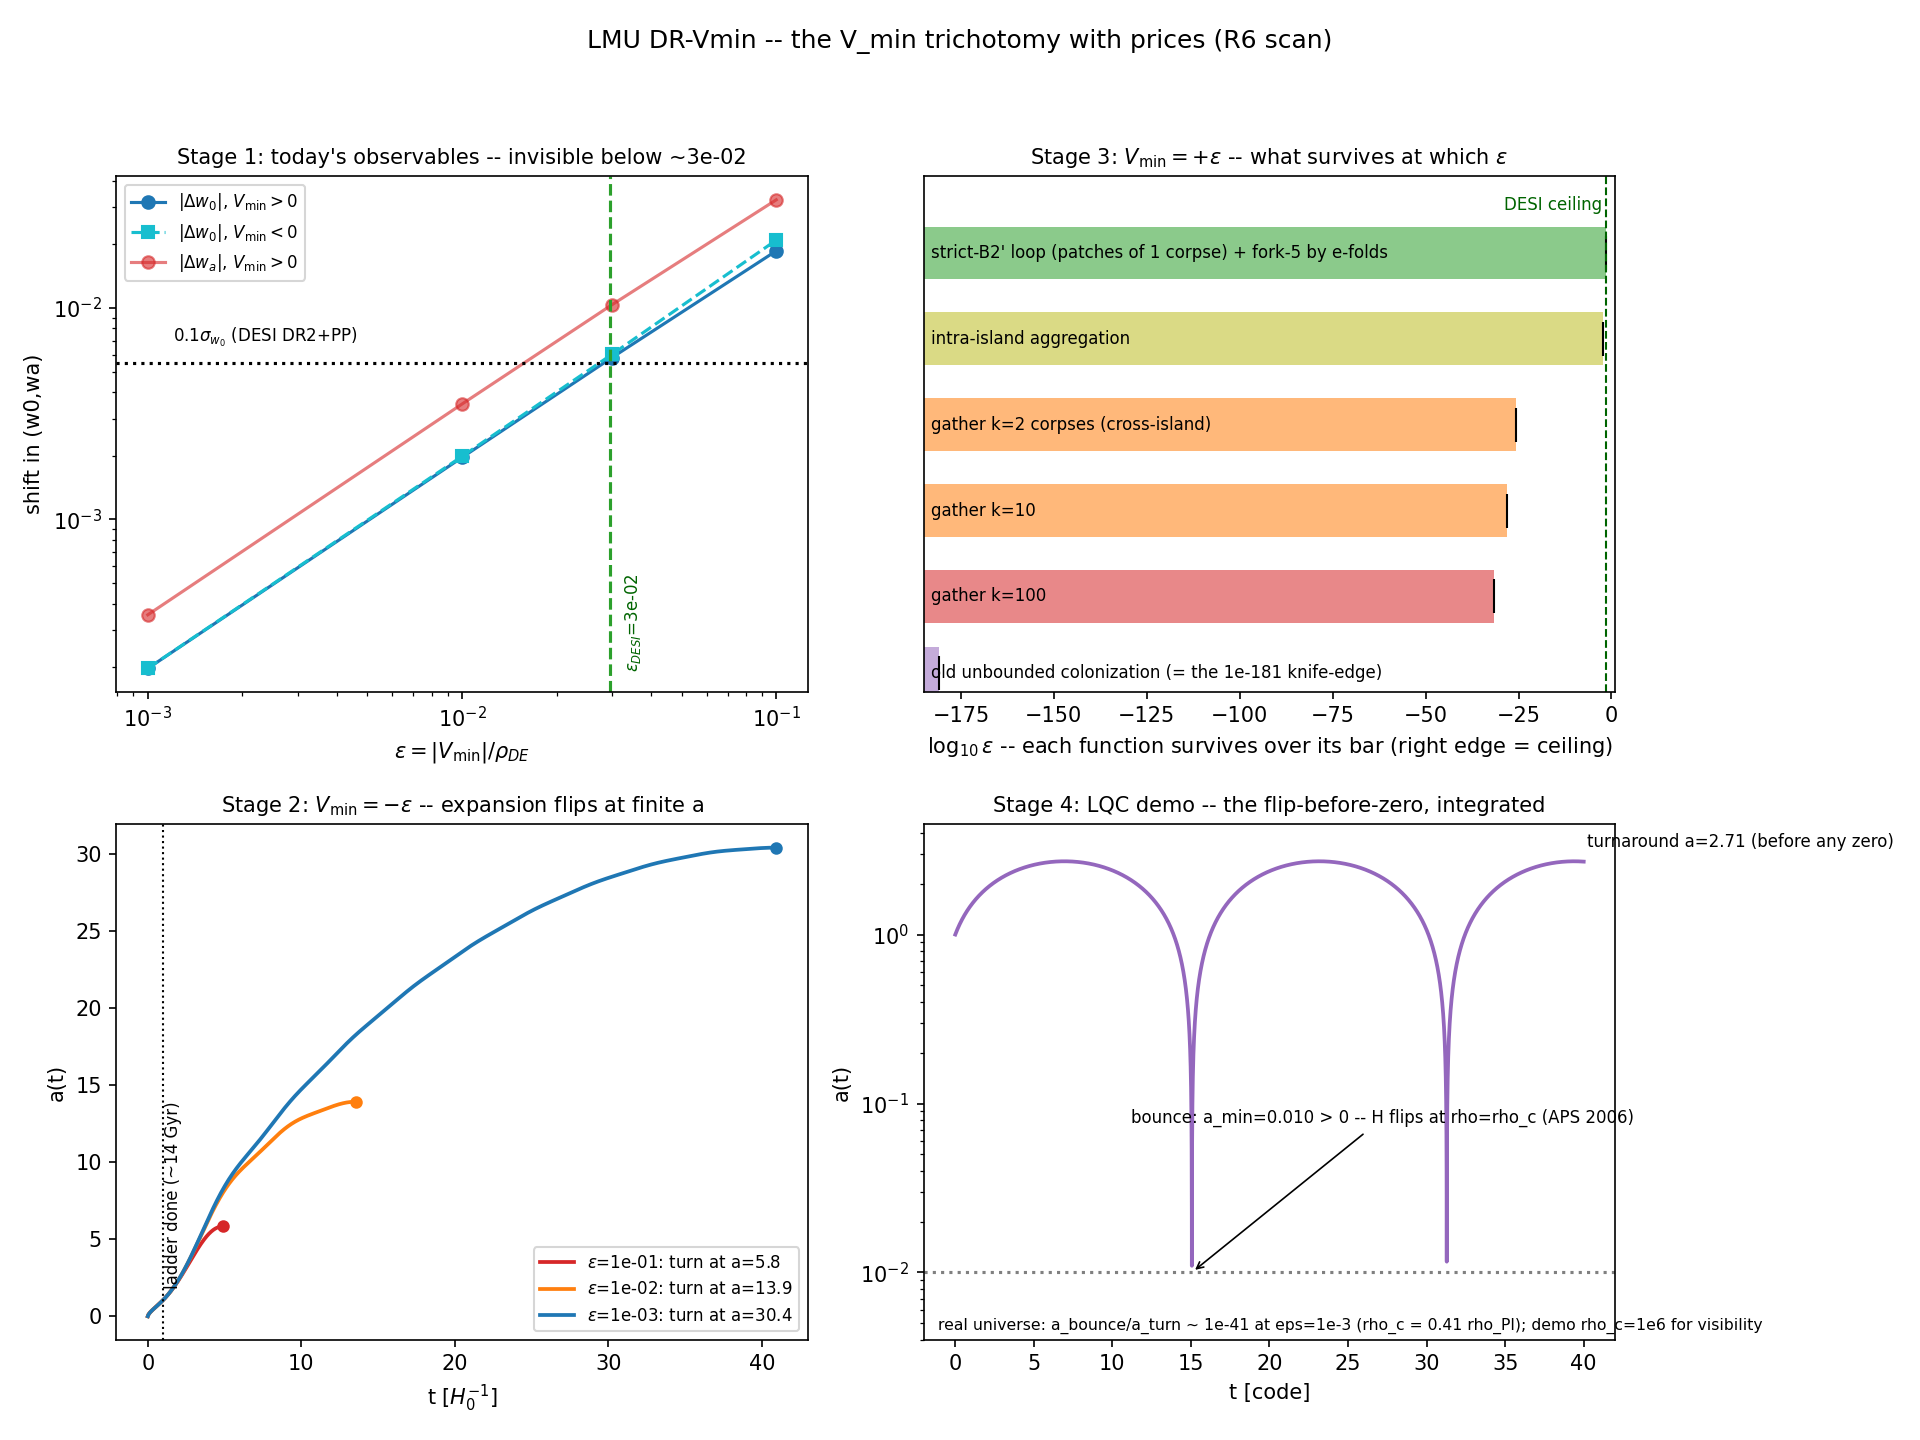
\includegraphics[width=0.99\textwidth]{dr_vmin_fork.png}
\caption{The trichotomy with prices: (a) observational invisibility below $\epsilon_{\rm DESI}=4.6\times10^{-2}$; (b) $+\epsilon$ survival ceilings; (c) $-\epsilon$ turnaround family; (d) the LQC bounce, integrated --- the flip before zero.}\label{fig:drvminfork}\end{figure}
\begin{figure}[h]\centering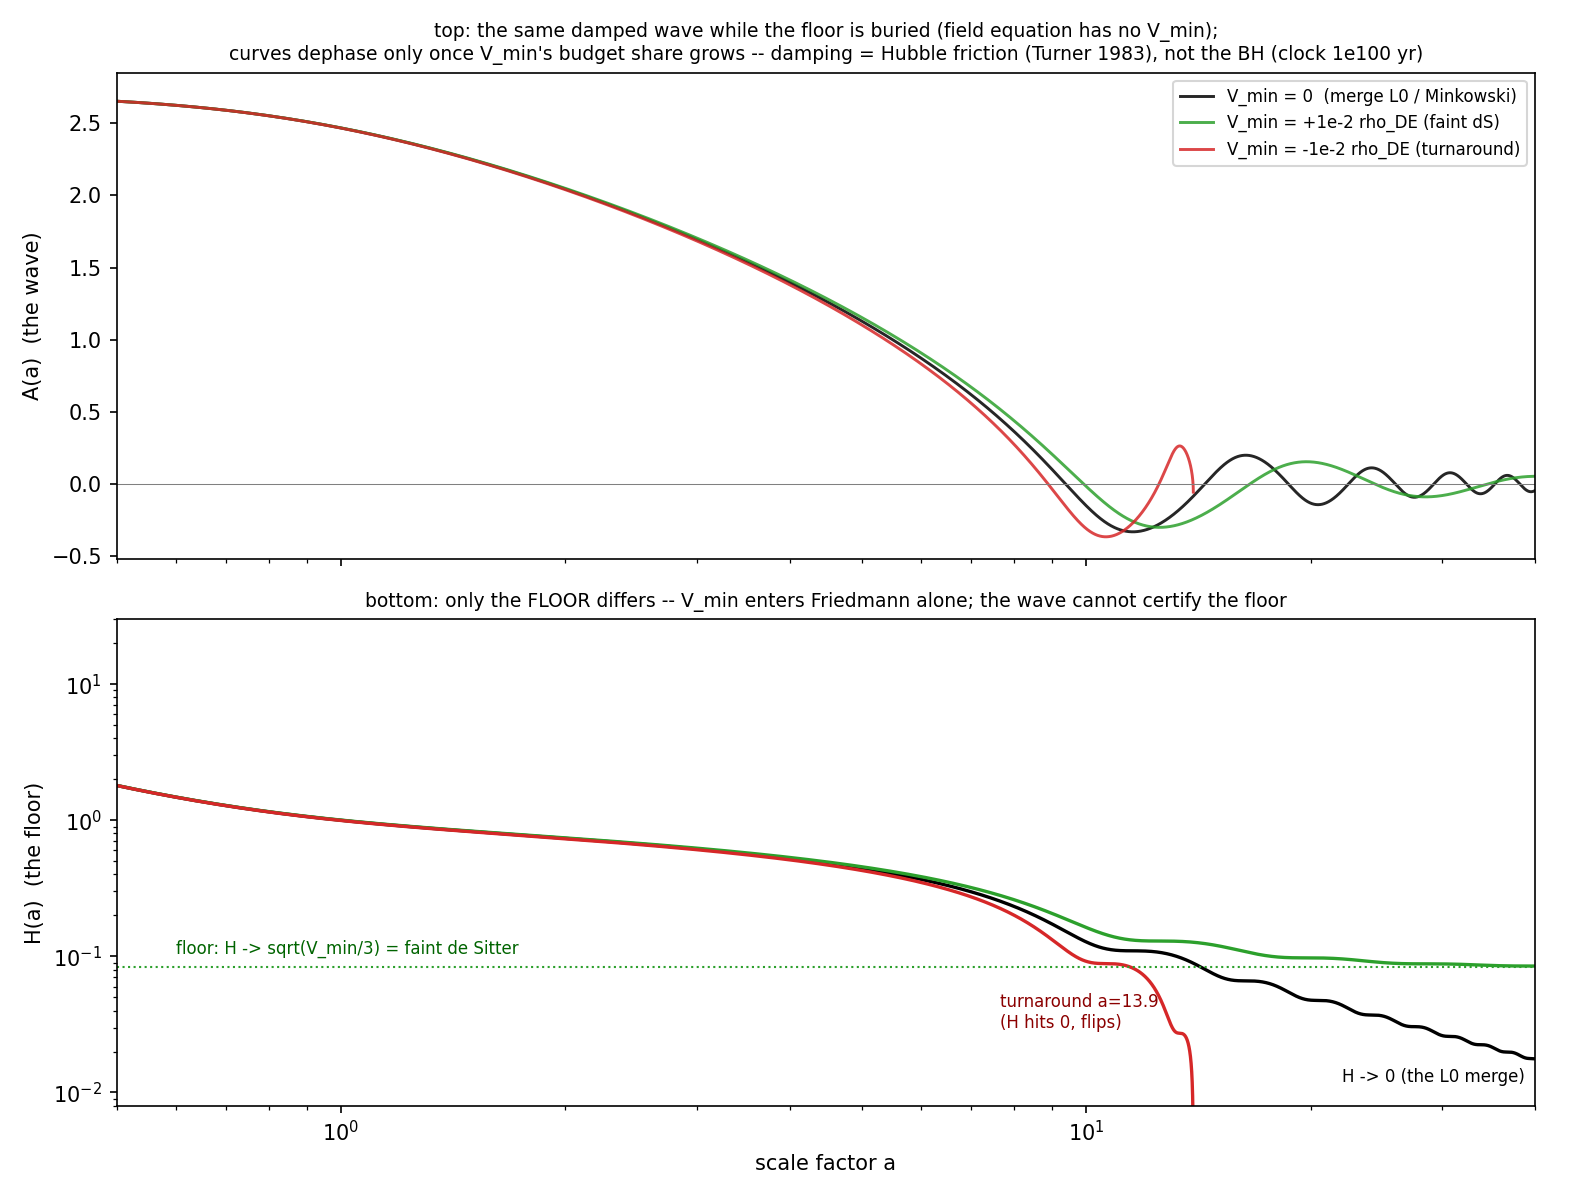
\includegraphics[width=0.92\textwidth]{endgame_three_floors.png}
\caption{Same wave, three floors: the field equation is $V_{\min}$-blind; only the Friedmann floor differs. The wave reveals the floor only when the endgame has already arrived --- the damped oscillation is evidence for all three branches equally.}\label{fig:threefloors}\end{figure}

\section{The fourth runner --- spatial curvature $\Omega_k$}
The endgame race had three runners (matter $a^{-3}$, floor $a^{0}$, shear $a^{-6}$); curvature ($a^{-2}$) was missing. Closed: turnaround at $a=D/(3|\Omega_k|)$; open: linear growth freezes under curvature domination (Peebles 1980). Ceilings on the $V_{\min}=0$ branch: first pairs free ($<1.24$); island hierarchy $<2.9\times10^{-18}$; eternity $<5.1\times10^{-60}$ ($\approx$68 e-folds of flattening per aeon, Guth 1981 scaling). At today's observational bound $|\Omega_k|\sim10^{-3}$, a closed sign crunches the interlude at $7.7\times10^{15}$\,yr. Consequences: the $V_{\min}=0$ branch carries \emph{two} knife-edges; $\Omega_k$ joins the B3$'$ re-init list (item I); the $+\epsilon$ branch is self-curing (dS e-folds re-flatten); $-\epsilon$ indifferent. Pattern note: this is again \textbf{Type-B} --- a known GR variable whose pricing converges on a mainstream requirement. \Auditor\ \textbf{Literature anchor (audit add):} Dinda \& Maartens (2025, MNRAS 542 L31; arXiv:2504.15190) fit thawing quintessence on a \emph{curved} background to DR2 and find it matches flat $w_0w_a$ --- the fourth runner is already a live, partially $w$-degenerate degree of freedom in the current data fits. \Fact

\section{Path 4 --- the per-zone reading}
$V_{\min}$ can be read as B3$'$ re-initialization \emph{data} rather than universal law: frozen vacuum draws per zone (landscape mechanism: Bousso--Polchinski 2000; Susskind 2003; the small-but-nonzero prediction: Weinberg 1987). $R_{\rm isl}\ge1107\,R_{\rm obs}$ hides per-zone variance three decades beyond any horizon --- isotropy data do not constrain it. The trichotomy then ceases to be a fork to choose: the population walks all three according to its distribution, and selection acts (flash-lineages out-reproduce bounce-lineages by $\sim10^{14.6}$ per generation). \hyp

\section{Path 4b --- cascade-to-zero (author wiring), and the absorbing state}
Vacua do not average by size; at any contact the \emph{lower} $V$ eats the higher through domain-wall/vacuum-decay dynamics (Coleman 1977; Coleman--De Luccia 1980). Two computed anchors: \textbf{(i) $L0$ at $V=0$ is a fortress} --- nucleating AdS of depth $\rho_{\rm DE}$ inside Minkowski is gravitationally blocked unless the wall tension is below $\sigma_{\rm crit}=5.8\times10^{16}$\,J\,m$^{-2}$ ($\approx(24\,{\rm MeV})^3$); every wall at or above the electroweak scale exceeds this by $10^{10}$--$10^{53}$ (a QCD-scale wall by only $\sim\!10^{2}$). \factth\ \textbf{(ii) $+\epsilon$ zones are genuinely pulled to 0}: dS$\to$Minkowski decay is allowed with thin-wall exponent $\log_{10}B\approx166$ (electroweak wall) --- the wait is $e^{10^{166}}$, glacial but finite against the branch's eternity, so $+\epsilon$ and $0$ merge asymptotically. \textbf{The cascade guarantees the destination, not the interlude} ($e^{10^{166}}\gg$ every loop deadline $\sim10^{107}$\,s); the tier table of \S2 still governs mid-flight. Why zero (and not a deeper floor) ends the cascade is the conjecture leg: non-SUSY AdS unstable (Ooguri--Vafa 2017), SUSY Minkowski uniquely stable (positive-energy theorem, Witten 1981). \hyp

\textbf{Absorbing state and the completed triad.} With a bounce-side re-draw of $V_{\min}$ (Wheeler reprocessing / Smolin CNS 1992; \hyp, item L --- plain LQC conserves the potential), every zone reaches $V=0$ through one of three doors: draw$\approx$0 merges directly (clock $\tau\propto M^3$); $+\epsilon$ evaporates, flashes, and its leftover vacuum is pulled (the cascade never pulls an L1 --- the survivor is $10^{(10^{166})}$-fold gone by then; L1 is a \emph{role}, not an object); $-\epsilon$ bounces and re-rolls until it exits to $\ge0$ (geometric waiting; per-zone Tolman accumulation capped as a side effect). Nothing draws exact zero --- zero is an \textbf{attractor}, consistent with the standing nothing-is-exactly-0/1 principle. Heredity completes the Darwinian triad: \emph{laws inherited perfectly} (children are patches of the corpse --- same $V_{\min}$, same constants), \emph{state re-rolled} (fresh $P(k)$); fertility $N_{\rm child}=1+g$ varies $\times4500$ with the zone's BH census --- the variance selection needs. Generative non-stillness is \emph{carried in by the corpse} (flash $+$ debris $+$ endowment), not grown from the void: Minkowski at $T=0$ births nothing real (vacuum-jitter rebirth would import the Boltzmann-brain pathology, Dyson--Kleban--Susskind 2002; Albrecht--Sorbo 2004); the one owned exception is the $+\epsilon$ far-future thermal channel (recycling universe, Garriga--Vilenkin 1998). Keystone --- \textbf{resolved-conditional (K1, 2026-06-11)}: the $\sigma_{\rm crit}$ fortress blocks only quantum nucleation; the classical account of \emph{born}-$-\epsilon$ zones closes with three locks (\texttt{k1\_wall\_accounting.py}; record \texttt{LMU\_K1\_wall\_accounting.md}). \textbf{(C) flat-space:} a wall grows only beyond $R^*=2\sigma/(\epsilon\rho_{\rm DE})$ (thin wall, Coleman 1977); island-scale $-\epsilon$ domains sit $R^*/R_{\rm isl}\ge1.6\times10^{10}$ \emph{below} growth for an EW wall at the DESI ceiling --- the tension crushes them inward (even a QCD wall clears by $\times3.6$ at the worst point, and the bound collapses to sub-eV$^3$ as $\epsilon$ falls). \textbf{(G) gravity (decisive):} any island-scale wall of tension $\ge$ QCD is in the Zel'dovich--Kobzarev--Okun 1974 catastrophic regime --- $R_{\rm isl}/R_{\rm grav}=1.4\times10^{6}$ (QCD) to $6\times10^{15}$ (EW), wall mass $10^{32}$--$10^{42}\,\msun$ deep inside its own Schwarzschild radius: planar walls repel (Vilenkin 1981; Ipser--Sikivie 1984), closed walls pinch off behind horizons (Blau--Guendelman--Guth 1987; Berezin--Kuzmin--Tkachev 1987), and exterior conversion is obstructed outright (Farhi--Guth 1987). Implosion, never invasion; the crunch ($2.2\times10^{11}$ yr at ceiling $\epsilon$) and island light-crossing ($5.1\times10^{13}$ yr) sit $\sim$86 orders inside the $10^{100}$-yr budget. \textbf{Two-sided ledger:} outside, the $-\epsilon$ zone deposits as an ordinary BH corpse ($\tau\propto M^3$, standard $L0$ furniture --- the vacuum book is never touched); inside, crunch $\to$ LQC bounce $\to$ re-roll --- \textbf{item (L) acquires its geometric home inside the collapse horizon, Smolin's native CNS setting}. \factth\ (the three locks) / \hyp\ (re-roll)
\begin{figure}[h]\centering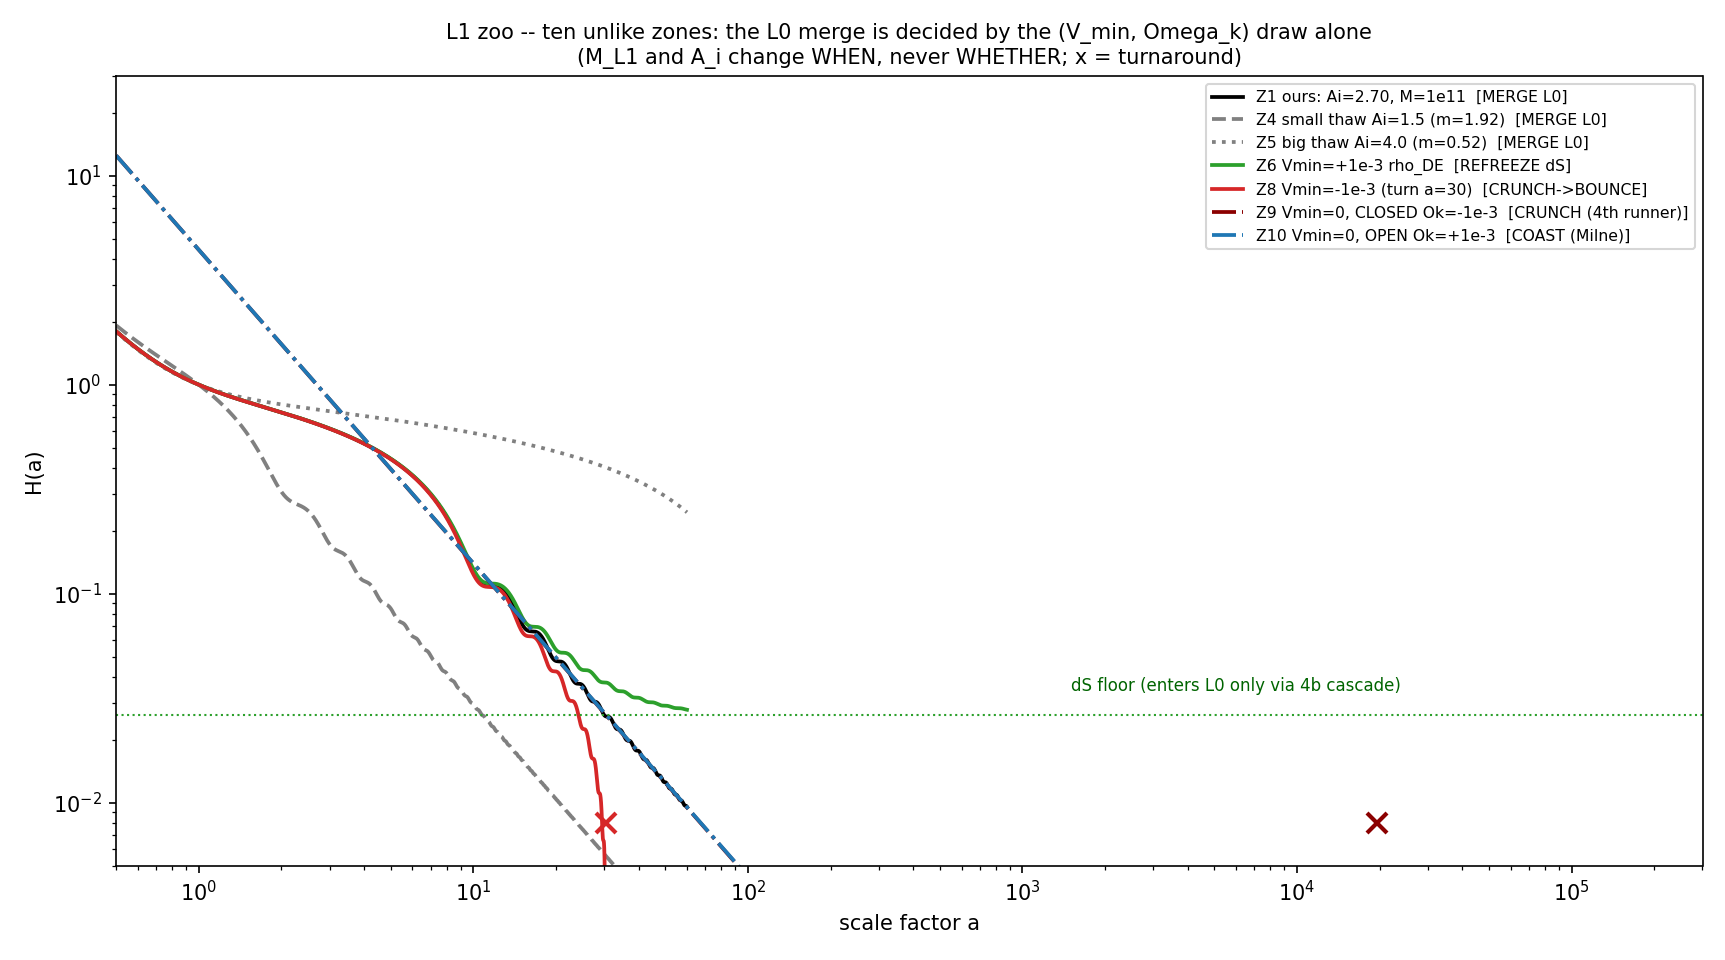
\includegraphics[width=0.95\textwidth]{l1_zoo_fates.png}
\caption{The L1 zoo --- ten unlike zones, integrated: \emph{whether} a zone enters $V=0$ at $L0$ is decided by its $(V_{\min},\Omega_k)$ draw alone; $M_{L1}$ and $A_i$ set \emph{when} ($\tau\propto M^3$), never whether. Late slopes check: dust $-1.500$, Milne $-1.032$.}\label{fig:zoo}\end{figure}

\section{Status, rulings required, and the audit trail}
\textbf{Ruling (item K, 2026-06-11):} paths 4$+$4b \textbf{adopted, conditional} --- the population walks all three branches by birth draw; $V=0$ is the selected attractor; K1 computed and closed (\S5). Spine numbers unchanged. What would reopen this: a sub-QCD-tension wall mechanism between vacuum draws, a failure of the bounce re-roll (L), or the why-zero conjecture leg falling (Ooguri--Vafa/Witten). If $-\epsilon$ is ever \emph{measured} ($w<-1$ sustained at DESI-Y5 with systematics resolved), the $B'$-replacement build spec opens regardless of this ruling. \textbf{Failure log of these sessions} (R4, carried in the session records): two file-write truncations (mitigated by chunked writes); the B16 tier conflation (corrected, \S2); $\epsilon_{\rm DESI}$ is now computed on the chain covariance ($4.6\times10^{-2}\,\rho_{\rm DE}$, joint $0.1\sigma$; the $0.1\sigma$-on-$w_0$ convention retired in V3.8); gathering ceilings are estimate-grade (Poisson seeds, $\delta_c=1.686$); one missed file-presentation step (checklist updated). Deliverable records: \texttt{LMU\_V3\_6\_STRESS\_TEST\_realdata.md}, \texttt{LMU\_DR\_Vmin\_trichotomy.md} $+$ addenda (curvature, 4b, absorbing state, triad). \Auditor

% ---------------------------------------------------------------------
\section{The (A)-window --- the crossing restored on the ruled spine}
Item (A) was the boundary problem of a zone at $V_{\min}=0$ \emph{exactly}: null $\mathscr I^+$, no Penrose/Eckstein crossing. Under the (K) ruling nothing draws exact zero (the attractor is approached, never sampled --- and exact zero has measure zero besides), so every lineage carries $\pm\epsilon'$: the $-\epsilon'$ half bounces inside its collapse horizon (K1) and never needs $\mathscr I^+$; the $+\epsilon'$ half ends de Sitter for \emph{any} $\epsilon'>0$ --- $H\to H_\infty=H_0\sqrt{0.69\,\epsilon'}$, conformal time $\eta=-e^{-H_\infty\tau}/H_\infty$, $ds^2=(H_\infty\eta)^{-2}(-d\eta^2+d\vec x^{\,2})$, $\mathscr I^+$ spacelike --- and the CCC machinery runs \emph{native} (Penrose 2010 itself requires $\Lambda>0$); this de Sitter end-state is the maximum-entropy attractor reached \emph{via} the generalized second law (Carroll \& Chatwin-Davies 2018), so the crossover smoothing runs \emph{with} the second law, not by the loss-of-degrees-of-freedom entropy reset that CCC requires (Penrose 2010). \factth

\textbf{The clocks (computed; \texttt{lmu\_A\_window.py}).} Vacuum domination at $a_{\rm dom}=(1.45/\epsilon')^{1/3}$, $t_{\rm dom}=t_0\,a_{\rm dom}^{3/2}$; the split $\boxed{\epsilon'_{\rm crit}=6.3\times10^{-181}}$ --- flash-in-dS above, flash-in-dust-then-dS below, \emph{both} admitting the slice --- re-derives the full-program tier of \S2 from the other direction (the same arithmetic, inverted). Evaporation is undisturbed everywhere on the grid ($T_H/T_{\rm dS}\ge10^{12}$; $M_{\rm Nariai}(H_\infty)\ge10^{23}\,\msun\gg$ band). The window $[\max(t_{\rm dom},\tau_{\rm evap}),\,t_{\rm decay}]\sim[10^{108}\,\text{s},\,e^{10^{166}}\,\text{s}]$ supplies $\sim e^{10^{166}}$ e-folds; the cascade rate $\Gamma\sim e^{-10^{166}}$ is hyper-subcritical, so the dS phase is globally future-eternal (eternal-inflation persistence) and un-decayed comoving patches are certain on the slice. \factth \textbf{Quantum-breaking caveat (V3.13).} The same lane that backs $V_{\min}=0$ (J2, Part~VI \S18) cuts against \emph{unconditional} future-eternity here: if de Sitter quantum-breaks (Dvali--G\'omez--Zell 2017), the usable budget is $N_Q\sim(M_p/H_\infty)^2$ e-folds --- R6-recomputed: $9.03\times10^{121}$ at $\epsilon'=\epsilon_{\rm DESI}=4.6\times10^{-2}$ and $6.60\times10^{300}$ at $\epsilon'_{\rm crit}=6.3\times10^{-181}$ (a species factor $N_{\rm sp}\sim10^{2}$ shifts the exponent by $-2$) --- replacing the decay-rate budget $\sim e^{10^{166}}$. The crossing itself is indifferent: it needs only $N=O(10^{2})$ ($e^{-2N}=10^{-87}$ at $N=100$), margin $\gtrsim10^{120}$; but ``globally future-eternal'' must be read as conditional on the absence of quantum breaking. \hyp\ (the cut) / \factth\ (the margin arithmetic).

\textbf{The drafted construction (equations first, proof later --- author doctrine).} Matching slice $\Sigma_N$ at $N$ e-folds past $\max(t_{\rm dom},\tau_{\rm evap})$: dust residual $\propto e^{-3N}$; Weyl-cleanliness met exponentially for any finite $N$, the rate set by the \emph{slowest} channel --- frozen super-horizon tensors at $e^{-2N}$ (electric) / $e^{-3N}$ (magnetic, the Tod-2007 jump channel $\partial_n B$); fluid-sourced Weyl $e^{-4N}$ (V3.9 erratum, computed). Crossing: $\hat g=\Omega^2 g$ with $\Omega=-1/(H_\infty\eta)$, reciprocal continuation $\hat\Omega=-1/\Omega$ (Penrose 2010), Tod matching conditions on $\Sigma_N$; per-patch scope unchanged from B2$'$ (child $i$ $=$ comoving ball $B_i\subset\Sigma_N$ holding exactly $S_{\rm fix}$); entropy invariant (B1$'$ unchanged); $z_{\rm aeon}(\epsilon')=T_{\rm reheat}/T_{\rm dS}(\epsilon')$ --- now \emph{parametrized} per zone, with $T_{\rm reheat}$ the same beyond-horizon irreducible as before. \design\ \textbf{Proof obligations (V3.9 status):} \textbf{P1} the Tod junction theorem for $(g,\hat g)$ on $\Sigma_N$ --- \textbf{FRW core closed} (V3.9): a component of EoS $w$ enters $1/a$ at $\eta^{3(1+w)}$, integer for every carried component; the oscillating $A$-residue makes the crossing exactly $C^{2,1}$ ($C^2$, the Einstein/FPX requirement, holds with zero margin; $C^3$ log-periodically blocked); the child bang is radiation-exact; the FPX hypotheses hold at the root window. \emph{Open remainder (reduced, V3.10)}: \textbf{G1} --- reciprocal gluing, now \emph{perturbative openness off the Kopi\'nski--Valiente Kroon 2022 conformally-flat matching point}; mismatch channels priced ([G1-h/B] automatic; [G1-E] $e^{-2N}$; [G1-j] $e^{-3N}$), conditional travelling: [G1-$\Omega$] (the $\hat\Omega$ prescription: Newman/Tod/Nurowski/Markwell--Stevens), now also absorbing the $C^{2,1}$ knife-edge --- [G1-d] \emph{closed} (V3.11): on the flat-conformal-class spine LT09 holds trivially and the kink constrains $\hat\Omega$ only; in the TT sector the LT09 ladder formalizes the horns (smooth horn passes, price $\pi_{ij}$; class horn $=$ impulsive-wave $C^{1,1}$ interface outside LT09 class~(i), amplitude $e^{-2N}$). \textbf{G2} --- contaminated-bang well-posedness, reduced to one named theorem (inhomogeneous radiation $+\Lambda+$ $w'=-2/3$ image $+$ regular-branch scalar, at $C^{2,1}$; nearest anchors Anguige--Tod 1999, Tod 2002 (scalar matter models, gr-qc/0209071), Tod 2007, Lee--Nungesser--Tod 2020), one computed condition (G2-c: the $t^{-1/2}$ stiff-branch amplitude vanishes on $\Sigma$), the named tool \emph{executed} (V3.11, [G2-d]: the Gover--Kopi\'nski--Waldron 2023 criterion --- every LMU passenger lands in an allowed trace slot, the dust-image is geometrized as $H^{\rm ext}$, and the stiff branch has no slot, so G2-c is doubly derived; cross-aeon stress matching inherits [G1-$\Omega$]) [math-GR, \open; records \texttt{LMU\_G1\_G2\_pass.md}, \texttt{LMU\_G1d\_G2d\_pass.md}]. \textbf{P2} --- \textbf{closed-conditional} (V3.9, horizon exile): $\Omega$ is global within a zone; every wall/$\partial B_i$ comoving scale exits the $H_\infty$ horizon in finite $N$, so the crossing region never sees them (item (C) closes on the same budget; falls with (K)). \textbf{P3} $P(k)$ through $\Sigma_N$ --- \emph{item (D), re-scoped by DR-P($k$) (ruled, V3.12)}: the spectrum is \emph{per-aeon}, not inherited --- the ruling formalizes the computation (all channels die at $e^{-2N}$/$e^{-3N}$/$e^{-4N}$; the slowest survivor is tensor, not adiabatic scalar --- wrong type and spectrum for $A_s$). Each aeon must therefore contain its own fluctuation generator [\open, named import]; targets it must hit: $n_s=0.9649\pm0.0042$, $A_s=2.1\times10^{-9}$, $r<0.036$ (BICEP/Keck 2021), $f_{\rm NL}^{\rm loc}=-0.9\pm5.1$, percent-level isocurvature (Planck 2018). Generator existence is \emph{necessary for loop closure}: no $\delta\sim10^{-5}$ $\Rightarrow$ no galaxies $\Rightarrow$ no ladder $\Rightarrow$ no next flash. \emph{Why the generator is separate \emph{and} plateau-type (V3.16, R6):} were the single $A$-field to serve as \emph{both} inflaton and present dark energy on its quadratic $V=\tfrac12 m^2A^2$, chaotic-inflation slow-roll gives $n_s\approx1-2/N$, so the observed $n_s=0.965$ forces $N\approx57$ and hence $r=8/N\approx0.14$ --- \emph{excluded} by BICEP/Keck ($r<0.036$); the same-potential unification is \emph{falsified by the tensor bound}, an independent and sharper reason than the $e^{-2N}$ transfer-suppression: the in-aeon generator must run a \emph{plateau} potential (Starobinsky $r\approx12/N^2\approx0.004$; $\alpha$-attractor), not the late-$A$ quadratic, so its separateness is \emph{forced}, not merely permitted (owners: BICEP/Keck 2021; Starobinsky 1980). Discount specific to this framework: horizon and flatness are already paid by the crossover (causal contact from the parent's infinite past; Penrose 2010), so the import is a \emph{generator}, not full inflation --- but a flash-as-seed shortcut is pre-blocked by the dead-end-log precedent (flash-as-DE died on 13--49 orders; same burden of amplitude $+$ spectrum $+$ Gaussianity applies). Wording rule, document-wide: the flash lights the \emph{pre-generator} start; the observed hot start (BBN/CMB) is lit by the generator's reheating. The transfer question survives only as the \emph{cleanliness side}: what leaks across must stay below $r<0.036$ and PTA stochastic-background limits --- both passed automatically at large $N$. Forced stance: \textbf{LMU predicts the absence of CCC-style Hawking points and concentric circles} --- horizon exile puts every other island's flash outside the horizon --- a clean, falsifiable departure from Penrose's CCC (claims: Gurzadyan--Penrose 2010; An--Meissner--Nurowski--Penrose 2020; mechanism: Meissner--Penrose 2025, arXiv:2503.24263 --- the GWE crossover; critiques: Moss--Scott--Zibin 2011; Jow--Scott 2020). \textbf{Sharpened (V3.13).} Meissner--Penrose 2025 upgrades Hawking points from claimed signal to \emph{structural requirement} of CCC's crossover (conformally smooth \emph{except} at Hawking points), making this falsifier symmetric: confirmed HPs falsify LMU's horizon exile; sustained nulls leave CCC's mechanism with an unfulfilled requirement. Detection status: contested --- An--Meissner--Nurowski--Penrose 2020 (MNRAS 495, 3403) claim $99.98\%$; Jow \& Scott 2020 (JCAP 03, 021) find $87\%$ ($\sim$$1\sigma$) after ring-size marginalization. \textbf{Stakes flag, mandatory:} a confirmed HP detection does not merely close DR-P($k$) --- it breaks horizon exile itself, re-opening item (C), the transfer side of (D), and P2; everything stamped ``rides (K)/(A)'' re-opens with it. The background map (the $c_3/c_4$ series) stands; perturbation-level cleanliness \open. (H1) gains its arena: the $+\epsilon'$ window is the future-side Aguirre--Gratton stage. No new debt --- conditions inherited verbatim from (K); if (K) falls, this falls with it. \Auditor

\clearpage
\part{Open ledger and dead-end pointers}
\setcounter{section}{0}\setcounter{equation}{0}\setcounter{figure}{0}

% ---------------------------------------------------------------------
\section{The open ledger (one list, no duplicates)}
\begin{itemize}[leftmargin=2.6em,itemsep=3pt]
\item[\textbf{(A)}] \textbf{Non-conformal rebirth --- resolved-conditional / drafted} (2026-06-11, rides the (K) ruling): under ``nothing draws exact zero,'' every lineage is $\pm\epsilon'$ --- the $-\epsilon'$ half bounces inside its horizon (K1, no $\mathscr I^+$ needed); the $+\epsilon'$ half ends de Sitter for \emph{any} $\epsilon'>0$, restoring the spacelike $\mathscr I^+$ that Penrose's and Eckstein's crossings require natively. Window computed: $\epsilon'_{\rm crit}=6.3\times10^{-181}$ (the full-program tier, re-derived inverted) splits flash-in-dS from flash-in-dust-then-dS; both admit the matching slice $\Sigma_N$; budget $\sim e^{10^{166}}$ e-folds; evaporation undisturbed ($T_H/T_{\rm dS}\ge10^{12}$). Equation set E1--E4 drafted with proof obligations P1--P3 (Part~VII \S7); P2 $=$ item (C) sharpened, P3 $=$ item (D) sharpened. \emph{Item (A) was the boundary condition of a zone that, under the ruling, never exists.} No new debt --- conditions inherited verbatim from (K). \factth\ (geometry) / \design\ (construction) \emph{Quantum-origin alternatives do not relieve this (V3.16):} replacing the rescale with a Vilenkin tunneling-from-nothing or a Hartle--Hawking no-boundary start does not solve Problem~A \emph{within} the loop --- both presuppose \emph{no} prior aeon and \emph{no} $L0$, so adopting either \emph{replaces} the framework (an isolated origin, no carry-through) rather than closing its joint. (\emph{By contrast}, the B-primary nucleation adopted in V3.21 is \emph{not} creation-from-nothing: a Coleman--De~Luccia bubble forms inside the \emph{existing} $L0$ substrate, with the basin debris and $L0$ density lumps as its genuine past --- the C5 spin-axis carry-through rides them --- so it closes the joint without discarding the prior aeon or $L0$; it is the in-loop joint, not a replacement of the framework.) Both no-boundary/tunneling starts face the Feldbrugge--Lehners--Turok 2017 unsuppressed-perturbation result (no lapse contour rescues the no-boundary path integral), only partially answered by Robin-boundary constructions (Di~Tucci--Lehners). Recorded so the route is not re-proposed as an in-loop fix. Owners: Vilenkin 1982; Hartle--Hawking 1983; Feldbrugge--Lehners--Turok 2017.
\item[\textbf{(B)}] \textbf{$V_{\min}=0$ vs.\ Weinberg 1989}: a QFT-level wall; classical intuition cannot reach it. \open\ \textbf{Priced (V3.7):} the interlude survives a residual $|V_{\min}|/\rho_{\rm DE}$ only below $4.3\times10^{-3}$ (first pairs) / $5.5\times10^{-56}$ (island hierarchy) / $3.1\times10^{-181}$ (full program to $\tau$) --- $\sim$59 decades beyond the classic $10^{-122}$ problem; in Planck units the floor must sit at $\sim10^{-303}$. Branches and a candidate dissolving mechanism: Part~VII-DR.
\item[\textbf{(C)}] \textbf{F2}: the explicit $x^\mu$/patch-boundary rule for lumps across a per-zone rescale. Sharpened by the (A)-window: the rule now lives on a concrete surface --- $\Omega$ regularity at $\partial B_i\subset\Sigma_N$ (obligation P2, Part~VII \S7) --- \textbf{closed-conditional} (V3.9, horizon exile: every finite wall/patch scale exits the $H_\infty$ horizon in finite $N$; rides the (K)/(A) budget, falls with (K)). \factth\ (geometry, conditional)
\item[\textbf{(D)}] \textbf{F3}: the $P(k)$ re-initialization mechanism --- \textbf{re-scoped by DR-P($k$) (ruled, V3.12)}: the spectrum is \emph{per-aeon}, not inherited (every transfer channel dies at $e^{-2N}$ or faster; the slowest survivor is tensor --- wrong type and spectrum for $A_s$). The open content is now the \emph{in-aeon fluctuation generator} [named import] with targets $n_s$, $A_s$, $r<0.036$, $f_{\rm NL}$ (P3, Part~VII \S7); the cross-$\Sigma$ side survives only as cleanliness bounds, passed at large $N$. \open\ (generator)
\item[\textbf{(E)}] \textbf{$\beta$ owner --- resolved} (2026-06-10): $\beta\approx0.7$ has no owner as an $M_\bullet$--$M_{\rm halo}$ slope; all owned values are $\ge1$ (Bogd\'an et al.\ 2018 $\approx$1.05, observed cluster end; Bassini et al.\ 2019 $1.35\pm0.15$, sims; Bandara et al.\ 2009; Ferrarese 2002; Li et al.\ 2024 lensing $\approx$1.7). The 0.7 matches the stellar $M_{*,\rm BCG}$--$M_{500}$ slope (Kravtsov et al.\ 2018) --- a relation mix-up. Band slope corrected to 0.15--0.27 dex/decade; the headline survives at the range's lower edge, the derivation is replaced (Part~V \S1). \fact
\item[\textbf{(F)}] \textbf{A-dust Jeans gate --- resolved-conditional} (2026-06-10): island scales are super-Jeans from oscillation onset for all $m\gtrsim0.14\,H_0$ ($R_{\rm isl}/\lambda_J=2.9\times10^3$ at the live point, growing as $a^{1/4}$); the A-dust clusters with $p\to1$, island modes re-enter at $a/a_{\rm osc}\approx2.6\times10^7$, and any seed $\delta\gtrsim10^{-52}$ collapses before $\tau$ (the Poisson floor alone exceeds the requirement by $\sim\!10^{42}$). The gate closes only for $m\lesssim0.13\,H_0$ via horizon exile ($>$100 e-folds of late inflation), a regime outside the DESI-thaw identification. The suppressed branch ($p=0.044$, $\times4\times10^2$) is scoped to sub-Jeans scales ($<0.38\,R_{\rm obs}$ comoving at onset). Conditional on $V_{\min}=0$ (item B); seed origin stays open in (D). Files: \texttt{lmu\_itemF\_jeans\_gate.py/.png}. \factth
\item[\textbf{(G)}] \textbf{F5 --- closed by retirement} (2026-06-10, author ruling): no constant-$\Lambda$ medium exists at any stage (dark energy is the A-field on the $L1$ cycle; $L0$ has $A\approx0$), so the F5 constant-$\Lambda$ source terms get no successor and the check-before-quote obligation is discharged by renunciation. $\rho^*\sim10^{-116}$ and $0.17\,M_\odot$ stay permanently quarantined in the retired table; fork-5 cross-island \emph{delivery} (Part~III \S2, coupling iv) is unaffected. Any future source terms are a new item, derived on the dust background. \design
\item[\textbf{(H)}] \textbf{Past-eternity --- decided} (2026-06-10): adopted as an axiom-level choice --- the population is eternal in both time directions, no global beginning; islands die and are born, locations shifting through matter/radiation exchange. Forward-eternity is free (branching $\ge1$); the past side is carried by the Aguirre--Gratton 2002 construction already cited in Part~V, with Borde--Guth--Vilenkin 2003 standing as the theorem the axiom must answer. \design
\item[\textbf{(H1)}] \textbf{The explicit construction} --- \textbf{drafted-conditional} (V3.8): anchor ruled (a) per-lineage (author, 2026-06-11); equations H-E1--H-E4 --- per-tree past eternal in proper time, \emph{finite in aeon count}; AG carries the arrow, FPX25 the metric continuation, never conflated. Obligations: \textbf{P1} (Tod junction; FRW core closed V3.9 --- the crossing is $C^{2,1}$, zero margin at $C^2$; the Tod-2007 obstruction channel is sourced at the computed $e^{-3N}$; remainder G1$+$G2 --- reduced V3.10, checks run V3.11: G1 $=$ perturbation off the KVK22 solved sector, [G1-$\Omega$] travelling ([G1-d] closed, merged into [G1-$\Omega$]); G2 $=$ one named theorem $+$ condition G2-c (doubly derived) $+$ [G2-d] executed) and \textbf{P4} (geodesic exhaustion; reduces to P1 $\wedge$ the KMS24--FPX25 dispute $\wedge$ LQC-effective, modulo wall-riding pathologies). Rides (K)/(A); falls with (K). \open\ (P1, P4)
\item[\textbf{(I)}] \textbf{$A_i=2.70\,M_p$ mechanism} (with $\eta$, $P(k)$, $\hat n$, and \textbf{$\Omega_k$ --- added V3.7, the fourth endgame runner}: the B3$'$ re-initialization data). \open
\item[\textbf{(K)}] \textbf{DR-Vmin --- ruled-conditional} (2026-06-11, author): paths 4$+$4b adopted --- $V_{\min}$ is per-zone birth data (variation), $V=0$ the dynamically selected attractor (cascade $+$ absorbing state), every pathway to $L0$ set by the $(V_{\min},\Omega_k)$ draw. Spine numbers unchanged (branch-blind below $\epsilon_{\rm DESI}$). \textbf{K1 wall accounting resolved-conditional} (Part~VII \S5): $-\epsilon$ zones cannot convert $L0$ --- quantum door blocked ($\sigma_{\rm crit}$), classical door crushed ($R^*/R_{\rm isl}\ge1.6\times10^{10}$ EW), gravity door catastrophic-to-self (ZKO; $R_{\rm isl}/R_{\rm grav}\ge1.4\times10^{6}$); outside $=$ BH corpse, inside $=$ bounce$+$re-roll. Conditions: walls $\ge$ QCD scale; thin-wall junctions; item (L); the why-zero conjecture leg. \design\ (the ruling) / \factth\ (K1)
\item[\textbf{(L)}] \textbf{Bounce re-roll of $V_{\min}$} (path-4b leg): plain LQC conserves the potential; the re-draw is Wheeler-reprocessing / Smolin-CNS class; K1 locates it geometrically inside the $-\epsilon$ collapse horizon --- Smolin's native setting. Ownership of the inside-the-horizon-universe picture itself: Pathria 1972 (Nature 240, 298) first; Pop\l awski 2010 (Phys.\ Lett.\ B 687, 110; 694, 181) the modern Einstein--Cartan bounce realization --- the $-\epsilon'$ branch is their setting with a re-drawn $V_{\min}$ added. \hyp

\item[\textbf{(M)}] \textbf{Island / aggregation-site mass function --- named open (V3.16).} Part~V computes the Gumbel band ($10^{10}$--$10^{11}\,\msun$) for a \emph{single} canonical-size island; the \emph{distribution of island sizes across $L0$} --- hence the $L1$ mass distribution over the whole population --- is uncomputed. Each island's $L1\sim M_*\ln N$ scales with its own draw count $N$, set by the size of the $L0$ aggregation site that seeds it (Part~III \S2); if small sites dominate by number, small-$L1$ islands outnumber large ones, with a hard floor at the Jeans scale ($M_{\rm floor}\approx6.4\times10^{5}\,\msun$, Part~V \S1) and a ceiling at the Gumbel maximum of the largest island. \emph{The gap is one-sided}: the transform from a mass function to the exact PDF of its most-massive draw is mature and general --- built for haloes from the \emph{exact} (not asymptotic) extreme-value distribution (Harrison \& Coles 2011, MNRASL 418, L20) and already run for a black-hole ceiling against $\Lambda$CDM number densities (Behroozi \& Silk 2018, MNRAS 477, 5382) --- so it returns the per-island survivor PDF for \emph{any} supplied draw count; what is missing is only the \emph{input}, the $L0$ aggregation-site size distribution (premise-dependent --- the reservoir's site sizes are not yet derived), after which the population $L1$ function is the per-island PDF weighted over that distribution. The open content is the \emph{aggregation-site size distribution}; it does not touch C3 (no $L1$ ignites a hot start) and reinforces, not strains, entropy-dilution (every $L1$ is negligible against an infinite $L0$). Owner: author (the question); extreme-value foundation --- Fisher--Tippett 1928 / Gnedenko 1943, applied-cosmology machinery --- Harrison \& Coles 2011, Behroozi \& Silk 2018. \open
\end{itemize}

\textbf{The four empirical joints of the ladder audit} live in Part~VI \S\S17--20 and are listed here only for the single-ledger view:
\begin{itemize}[leftmargin=2.9em,itemsep=2pt]
\item[\textbf{(J1)}] super-Eddington feedback --- ``trapping despite outflow,'' not ``evades'' (Part~VI \S17). \open
\item[\textbf{(J2)}] the sign of $V_{\min}$ --- the framework sits on the less-favoured fork; same observable as (B)'s data side (Part~VI \S18). \open\ \textbf{Mapped (V3.7):} all three branches are observationally identical today below $\epsilon_{\rm DESI}=4.6\times10^{-2}$ and share the DESI-Y5 falsifier; the discriminators are theoretical economy, not near-term data (Part~VII-DR). \textbf{Identity guard (R9, V3.14):} the three branches are the \emph{one} $V_{\min}$-sign parameter read through field \emph{turn-around} --- a thaw-then-freeze $A$-field that turns \emph{gently} stops at $w\!=\!-1$ ($\rho_{\rm DE}\!\to\!{\rm const}\!>\!0$, de Sitter, $V_{\min}\!>\!0$, the conformal rescale native --- Penrose); turns \emph{exactly} oscillates to $\langle w\rangle\!=\!0$ ($\rho\!\propto\!a^{-3}$, Minkowski, $V_{\min}\!=\!0$, item~(A)/Problem~A); turns \emph{hard} settles toward $V_{\min}\!<\!0$ so $\rho_{\rm DE}$ goes negative (AdS) and the zone recollapses --- not by $w\!<\!-1$ (canonical scalars never cross; Vikman 2005) but by negative density --- landing on item~(L) (Pop\l awski / LQC bounce). ``Thaw--freeze'' is therefore \emph{not} a fourth runner but this same fork seen through dynamics; any future ``thaw--freeze fix'' must be checked against (J2)/(K)/(L) before being logged as new. \Auditor \textbf{Phantom-crossing correction (V3.14, owed):} the $w\ge-1$ bound is specific to a \emph{single canonical} scalar (Vikman 2005); phantom crossing \emph{is} reachable from the field equations, and is a \emph{genuine} fourth runner distinct from the $V_{\min}$-sign fork --- its endgame is $w<-1$ (super-acceleration), not de Sitter / Minkowski / AdS. Routes, each with a stated price: a two-field \emph{quintom} (Feng, Wang \& Zhang 2005; review Cai et al.\ 2010), whose phantom component carries a wrong-sign kinetic term --- a ghost (Carroll, Hoffman \& Trodden 2003); \emph{non-canonical / $k$-essence} kinetics (Armend\'ariz-Pic\'on, Mukhanov \& Steinhardt 2000), an added free function; or a coupling / modified-gravity \emph{effective} crossing (no real field crosses). The adopted $A$-field is canonical \emph{by choice}, so it stays pinned at $w\ge-1$: should DESI/Euclid establish a \emph{true} phantom crossing (not the CPL artefact of Dinda--Maartens 2025), the canonical $A$-field falls (F1) --- but a quintom/$k$-essence upgrade survives, at the cost of a ghost, an extra degree of freedom, and the loss of the ghost-free-canonical economy that motivated $A$ in the first place. Recorded as a fourth fork so it is neither overlooked nor conflated with the $V_{\min}$ branches. \Auditor
\item[\textbf{(J3)}] $f_{\rm coh}$ coherence --- ``conditional, against the trend,'' not ``mild'' (Part~VI \S19). \open
\item[\textbf{(J4)}] the engine and the spin condition pull against each other --- the composite ``coherent-but-trapped'' window (Part~VI \S20). \open
\end{itemize}
With the M87 contested-spin (\open) flag (Parts I, V, VI) attached wherever the ladder is reused.

% ---------------------------------------------------------------------
\section{Dead-end pointers (check before extending anything)}
\textbf{A1} --- DM origin, killed $\times5$ (Bullet Cluster $+$ timing $+$ 5:1); correct form: thermal relic re-minted each aeon. \textbf{(2026-06-26 refinement, R7-verified):} the ``survivor cracks open to release a compressed dark-matter residue'' sub-route stays dead --- it needs the late $L1$ survivor (or its $L0$ lump) to shed an interior core without normal evaporation, which no-hair forbids (no core; cf.\ C2) and timing blocks (the lump evaporates in the reservoir \emph{before} the child aeon, so only massless radiation crosses, yet dark matter must be present by the child's recombination). The literature's \emph{working} mechanism is the opposite object --- dark matter from \emph{normal} Hawking evaporation of \emph{fresh, early} child-aeon primordial black holes (Regurgitated DM, Kim--Lu--Marfatia--Takhistov 2024; PBH-evaporation DM, Cheek et al.\ 2022; Recycled DM, Gehrman et al.\ 2024) --- a citeable alternative to thermal freeze-out available only to early child PBHs, never the survivor. The in-zone survivor, the same mass as its $L0$ lump, and a fresh child PBH are three distinct objects; the dead route lives at the first two, the working literature at the third (record \texttt{LMU\_terminology\_L1\_vs\_L0lump\_vs\_childPBH\_2026-06-26.md}). \dead\quad
\textbf{A2} --- DE/$\Lambda$ origin: rotation/vorticity (Saadeh et al.\ 2016 kills), Hawking-tail-as-DE, flash-as-A-source (short by 13--49 orders) --- all dead; in the current framework dark energy is the A-field, no constant remains. \dead\quad \textbf{A2-GW (V3.15)} --- cosmic acceleration read as the tidal stretch of riding one half-cycle of a giant $L1$--$L1$ merger's gravitational wave: \textbf{dead $H$-independently}, on four counts no choice of source mass or epoch repairs. \emph{(i) Energy sign}: a gravitational-wave background carries \emph{positive} energy and redshifts as radiation, $w=+\tfrac13$ (Isaacson 1968), so it \emph{decelerates}; the acceleration condition $\rho+3p<0$ fails by the wrong sign ($\rho+3p=2\rho>0$). \emph{(ii) Tensor rank}: GWs are transverse-traceless \emph{quadrupole} radiation while cosmic acceleration is isotropic --- a \emph{monopole}; there is no monopole gravitational radiation (Birkhoff 1923), a mismatch of tensor type neither $M$ nor $H$ can mend. \emph{(iii) Frozen super-horizon}: a half-cycle spanning the acceleration epoch has wavelength $\sim$ the Hubble radius --- super-horizon, where tensor modes are \emph{frozen}, not an oscillating usable tide (Grishchuk 1974). \emph{(iv) Budget}: $\Omega_{\rm GW}\sim10^{-9}$ (PTA-scale SGWB) down to far less, against $\Omega_{\rm DE}=0.69$ --- short by $\sim$9--15 orders; a source giant enough would need $M\gtrsim10^{22}\,\msun$ (Nariai during $A>0$), forbidden. The accelerant stays the thawing $A$-field (Result~3); the merger's waves are an ordinary $\propto a^{-4}$ radiation channel, already booked at Part~III \S2 ($\sim$5--10\% of rest mass, to infinity), \emph{not} dark energy. Owners: GW stress-energy --- Isaacson 1968; super-horizon freezing --- Grishchuk 1974; monopole no-go --- Birkhoff 1923. \dead\quad


\textbf{Scale check (A2 reinforced).} At star-forming (ISM) scales --- molecular clouds, $\sim$pc to $\sim$100\,pc --- the matter energy density exceeds $\Lambda$ by $\sim\!10^{8}$--$10^{11}$ (clouds to dense cores), so dark energy plays no dynamical role in collapse (gravity vs.\ Jeans pressure only); and $\Lambda$ does not clump (it is, relatively, \emph{void}-dominant). Consistently, the A-field clusters only on super-Jeans (island) scales: ISM scales lie $\sim\!10^{8}$ below the comoving $\lambda_J=1.68\times10^{26}$\,m, deep in the pressure-supported (smooth) branch. So neither real DE nor the model's A-field localizes into star-forming structure --- the ``DE concentrates where structure forms'' route stays dead (A2). \Auditor

\textbf{B} --- gravity-beats-expansion: \textbf{now scoped} --- valid only during the acceleration window; void on the dust interlude (Correction 1). Mid-aeon baryogenesis stays dead (hot boundary only). \dead/\design\quad
\textbf{B-W} --- Weyl-residue disposal/repurposing (both directions dead). \emph{Disposal}: cancellation or absorption of the frozen $E$/$\partial_n B$ residues dies on (i) super-horizon causality, (ii) incoherent power addition (stochastic GW add in power, never subtract), (iii) category --- the gap is mathematical (the Anguige--Tod class demands exact zero), so any ``reduce the residue'' mechanism is structurally redundant against the unlimited e-fold budget. \emph{Repurposing} (residue as asymmetry seed): dead on the DR-P($k$) ruling (slowest survivor is tensor --- wrong type/spectrum for $A_s$), on scaling (a knob flowing to zero with $N$ cannot set a constant; $\eta$ sits at B3$'$, Sakharov per round), and on the Weyl Curvature Hypothesis (Penrose 1979) running the \emph{opposite} way --- the arrow lives in the residue's smallness, not in the residue. Residues have one job: pricing the G1 perturbation. \dead\quad
\textbf{CCBH} (Croker--Weiner; Farrah et al.\ 2023): context, coupling scoped off on the spine; R8 applies to rebuttals.

\medskip\noindent\textbf{Hot-start-from-matter wall (unifying --- check before proposing any new ignition mechanism).} Any hot start built by \emph{heating real matter} --- compression, collision, infall, or a released dense ``core'' --- fails on one of two walls. \emph{Hoop wall}: matter dense enough for baryogenesis ($T\gtrsim10^{15}$\,K, the electroweak floor) lies inside its own Schwarzschild radius and collapses to a cold hole, not a fireball (Thorne 1972); the motion is inward (collapse), the wrong sign for an expanding hot start. \emph{Energy-budget wall}: the $A$-field, being dark energy, carries only $\sim$meV, so any field-driven reheating is capped far below threshold. The only mechanisms that evade both touch \emph{geometry or vacuum, not matter}: \textbf{bubble nucleation} from the $\Phi_{\rm gen}$ false vacuum (B-primary --- an open Coleman--De~Luccia interior inflates and reheats; its heat is vacuum energy released by reheating, not heated matter), the conformal rescale (needs de Sitter $\mathscr I^+$ --- the (A)/(K) program; B-alt), a Planck-density bounce (imports LQC/torsion --- item (L)), or a brane collision (imports extra dimensions --- dead). \Auditor

\medskip\noindent\textbf{Problem~A under the two joints --- the shared residual (Layer~C, V3.21).} The matter routes below (C1--C5) stay dead exactly as logged. What V3.21 changes is only the \emph{surviving} route: it is no longer uniquely ``the rescale'' but a \emph{vacuum-route family} --- nucleation (B-primary) or conformal rescale (B-alt). Wherever an entry below reads ``the matter-free rescale remains the only route,'' read instead ``a vacuum route remains the only family; nucleation is the primary member.'' \emph{What the residual now is.} Under B-primary the energy face \emph{dissolves}: the $\sim\!10^{22}$ gap between a child's content ($\sim\!2\times10^{80}$\,J) and a survivor's flash ($\sim\!1.8\times10^{58}$\,J) is not paid but removed, because an inflating bubble interior grows $E=\rho V$ at no net cost (the inflationary free lunch) and is super-horizon, fed by no $L0$ inflow (Part~IV, B-primary). What remains to posit is one thing only: that the $\Phi_{\rm gen}$ false vacuum (item~D) exists and is accessible at $\sim\!10^{16}$\,GeV in a small patch --- \emph{the inflaton-level posit of standard inflation}, no more and no less. \emph{Honest line.} This is the field-wide cosmological-constant / initial-condition frontier (Weinberg 1989), not an LMU-specific defect; V3.21 does \emph{not} climb that wall --- it re-anchors the residual and posits it \emph{once}, used by both joints. It is not a breakthrough; it is a relocation of the same irreducible posit. \hyp\ (the $\Phi_{\rm gen}$ false-vacuum branch is accessible) / \open\ (the measure / why-now).

\textbf{C1} --- $A$-field potential reheating as a substitute for the conformal blueshift: \textbf{dead, by $\sim$55 orders}. \emph{Idea}: let $A$, on reaching $V$'s floor, release latent heat (inflaton-style reheating; Kofman--Linde--Starobinsky 1994) to fire the hot start, removing the de-Sitter dependence of item (A). \emph{Where it breaks}: the $A$-field \emph{is} dark energy, so its whole density is $\rho_{\rm DE}\approx\Omega_\Lambda\rho_{\rm crit}$, scale $\rho_{\rm DE}^{1/4}\approx2.24$\,meV; thermalizing all of it gives $T_{\max}\approx26$\,K against a $\gtrsim10^{15}$\,K (electroweak) need --- short by $\sim$14 orders in $T$, $\sim$55 in energy density. With $m\sim H_0\sim10^{-33}$\,eV it is the coldest field in cosmology, and a high-energy false vacuum bolted onto $V$ is no repair (it gives a GUT-scale $\Lambda$ today, excluded). \emph{Survivor}: none --- the temperature is supplied by the rescale (geometry; $\Omega^{-1}\sim10^{47}$ multiplies $T$ with \emph{no} energy present), which is exactly why no $A$-field reheating can replace it. (R6: recomputed from $G,H_0,\Omega_\Lambda,c,\hbar,k_B$; nothing inherited.) Owners: reheating --- Kofman--Linde--Starobinsky 1994; $m\sim H_0$ quintessence --- Ratra--Peebles 1988. \dead\quad

\textbf{C2} --- a dense ``core'' released from the survivor at end-of-evaporation, triggering collapse-and-collision: \textbf{dead twice}. \emph{(a) unitarity / no-hair}: by the framework's own commitment evaporation leaves no remnant (the full $M_{\rm bh}c^2$ returns as radiation; a Kerr--Newman hole has no interior ``core''), so importing one overturns the unitarity stance the boundary rests on. \emph{(b) hoop wall}: a ``hyper-dense object that warps spacetime sharply'' \emph{is} a black hole, and infalling $L0$ material crosses a horizon as gravitational waves, not into an open-space fireball --- the hot-start-from-matter wall above, re-entered from a new door. The motion is collapse, not expansion. \emph{Survivor}: none. Owners: no-hair / no-remnant --- Hawking; hoop --- Thorne 1972. \dead\quad

\textbf{C3} --- the single survivor set to \emph{infinite mass} ($M_{L1}\to\infty$) as the ignition --- ``make the last hole so big it never needs the rescale'': \textbf{dead on three facts at once, and unnecessary}. \emph{Idea}: if one survivor carries unbounded mass it could (the thought runs) skip the de-Sitter--Minkowski gap of Problem~A. \emph{Where it breaks}: \emph{(a) Hawking clock} --- the lifetime $\tau_{\rm evap}\simeq2.1\times10^{67}(M/\msun)^3$\,yr (already $2.1\times10^{217}$\,yr at a merely illustrative $10^{50}\,\msun$) makes $M\to\infty\Rightarrow\tau\to\infty$: the hole never evaporates, never reaches the Penrose turning point, the flash never fires --- the loop \emph{cannot close}, the decisive kill. \emph{(b) Friedmann constraint} --- $3H^2=8\pi G\rho$ ties the reservoir's $H\to0$ endgame to $\rho\to0$ (the same equation that lifts the Nariai ceiling, $H\to0\Rightarrow M_{\rm Nariai}\to\infty$, Part~III \S1); a literally infinite \emph{localized} $\rho$ is the opposite of the $\rho\to0$ background it must evaporate into --- one equation, contradictory readings. \emph{(c) Hoop reach} --- $R_s=2GM/c^2\propto M$ diverges ($R_s/R_{\rm obs}\sim10^{27}$ already at $10^{50}\,\msun$), overrunning every causal patch including the island bound $R_{\rm isl}=1107\,R_{\rm obs}$, so an ``infinite survivor'' is not an object inside a zone at all. The Nariai ceiling \emph{alone} permits $M\to\infty$ at $L0$ ($H\to0$), but permission by one bound is not realization: the operative survivor bound is extreme-value (Part~V \S1), logarithmic in $N$, holding the band finite. \emph{Resolution} (no new mechanism): mass is unbounded in the \emph{count of islands} --- the eternal population, each $L1$ finite in the $10^{10}$--$10^{11}\,\msun$ band --- never in a single survivor; ``infinite mass'' lives in fork~5, not in any one hole, so the $\infty$-single route is both impossible and superfluous. \emph{Survivor}: none. Owners: lifetime/turning point --- Hawking 1975; Page 1976; constraint --- Friedmann 1922; $R_s$ --- Schwarzschild 1916; eternal-population resolution --- the existing fork~5 / Aguirre--Gratton 2002. \dead\quad

\textbf{C4} --- \emph{energy/event-based ignition} (this session's adversarial sweep, 2026-06-22): the hot start is \emph{lit by a physical event in $L0$} --- Hawking radiation pooling and sparking, two survivors colliding, or mass accumulating until spacetime ``dumps.'' All \textbf{dead on one shared budget fact}, three doors checked. \emph{(a) Leak-and-spark} (Hawking radiation concentrates then ignites): the survivor's emission is the coldest source in the model ($T_H\sim6\times10^{-19}$\,K) and enters a reservoir that \emph{dilutes} ($\rho\to0$) --- the opposite of pooling --- and even fully re-concentrated, one survivor carries $M_{L1}c^2\approx1.8\times10^{58}$\,J ($10^{11}\,\msun$) against a child matter content $\sim2\times10^{80}$\,J, short by $\sim$22 orders. This is C1/A2 re-entered: the energy is supplied by the rescale (geometry), never by the radiation. \emph{(b) Collision trigger} (two $L1$ ``shells'' collide and set something off): a black hole has \emph{no shell} --- no-hair leaves only $(M,a_\star,Q)$ --- so there is no surface to react; and $L1+L1$ is a \emph{merger}, $A_{\rm final}\ge A_1+A_2$ (Hawking area theorem; LIGO-observed $\sim$100$\times$), yielding a \emph{larger, colder} hole plus $\sim$5--10\% in gravitational waves, never a fireball --- bigger $M\Rightarrow$ longer $\tau\Rightarrow$ \emph{farther} from ignition. Flipping the collision's collapse into expansion needs NEC violation (a bounce import, item~(L)), not the collision itself. \emph{(c) Spacetime ``dump''} (mass accumulates until the metric ``cannot bear it'' and releases): GR has no container and no overflow --- concentrated mass curves space \emph{inward}, and past the hoop it forms a horizon (a BH), it does not spill. This is C3 wearing the rubber-sheet misconception (the sheet needs an external ``down''; real spacetime has none). \emph{Unifying verdict}: every energy/event ignition fails \emph{identically} because the largest carried object ($\sim$one galaxy-scale survivor) sits $\sim$22 orders below a whole aeon's energy content --- a structural deficit no arrangement, collision, or pooling repairs --- and \emph{mass-independent} besides: compressing matter to its own Schwarzschild radius gives a virial ceiling $kT_{\rm vir}\sim\tfrac{1}{10}m_pc^2$ (virial convention $T=GMm_p/(5k_BR)$ at $R=R_s$; escape speed $=c$ at $R_s$ for \emph{any} $M$), i.e.\ $T_{\rm vir}=m_pc^2/10k_B\approx1.09\times10^{12}$\,K with the mass \emph{cancelled} --- short of the $\gtrsim10^{15}$\,K baryogenesis threshold by $\sim$3 orders ($918\times$), so no choice of survivor mass reaches ignition (R6, this session) --- exactly the ``hot-start-from-matter wall'' above seen from the $L0$ side. The matter-free rescale (Problem~A) remains the only route, and remains open. Owners: no-hair / area theorem --- Israel 1967, Hawking 1971/1975; hoop --- Thorne 1972; GW energy --- Isaacson 1968; NEC/bounce --- LQC (item~(L)). \dead\quad

\textbf{Finite-$L0$ (closed-box bounce)} --- replacing the infinite reservoir (fork~5) $+$ conformal rescale with a \emph{finite, boundaryless} $L0$ that accumulates to a density ceiling and bounces (LQC/torsion): \textbf{dead on the Weyl channel --- three independent walls converge} (exploratory fork, 2026-06-24). \emph{Idea}: form-convert entropy (cold$\to$hot by accumulation in a sealed box) rather than dilute it, so the unprovable infinite premise is removed --- the box fills to $\rho_c$ and a beyond-GR term drives $(\rho+3p)_{\rm eff}<0$, forcing re-expansion without a reset. \emph{Where it breaks}: a low-Weyl (smooth) hot start needs the gravitational-clumping entropy removed before the bang, and a finite box closes the only channel that does it. \emph{(a) GSL / gravothermal}: a self-gravitating system has no maximum-entropy equilibrium and its high-density attractor is the black hole (Antonov 1962; Lynden-Bell \& Wood 1968), so the $\mathrm{BH}\!\to\!$radiation conversion that turns Weyl entropy into smooth thermal entropy is entropy-\emph{increasing} only below a crossover $\rho_{\rm cross}\!\approx\!6\times10^{-104}$\,kg/m$^3$ ($S_{\rm BH}\!=\!S_{\rm rad}$ for a $10^{11}\,\msun$ lump); above it $S_{\rm BH}\!>\!S_{\rm rad}$ (by $\sim$50 orders for one survivor at the Planck-scale ceiling, $\sim$185 for the merged population), so evaporation \emph{reverses} --- and a box that must climb to the ceiling spends essentially the whole climb on the forbidden side. \emph{(b) Hawking--Page}: the bath at the ceiling reaches $\sim10^{22}$--$10^{32}$\,K (torsion vs.\ LQC), $\gtrsim10^{40}$ hotter than a survivor's $T_H\!\approx\!6\times10^{-19}$\,K, so by negative heat capacity the survivors \emph{absorb and grow}, not evaporate (Hawking--Page 1983; York 1986) --- the lumps reach the floor. \emph{(c) no-hair}: $L0$ inherits $10^{11}\,\msun$ survivors from the ladder, and a hole cannot be un-made except by evaporation (Israel 1967; Carter 1971), which (a)/(b) close --- so the pre-formed lumps ride the bounce and the bang is born at \emph{maximal} Weyl, contradicting the observed near-perfect CMB smoothness (Fixsen 2009; Penrose's low-Weyl initial condition, 1979). \emph{Why this confirms the canonical}: the infinite/dilute reservoir is the \emph{only} regime where evaporation is GSL-favored (below $\rho_{\rm cross}$) \emph{and} the bang is built from massless radiation alone with the lumps stashed in $L0$, never entering the boundary --- a finite box has no outside to stash lumps in, so it must push them through the bounce, where nothing smooths them. The torsion ceiling $\rho_c^{\rm tor}\!\approx\!5\times10^{57}$\,kg/m$^3$ (from the fermion Cartan density $n_c\!=\!mc^4/2\pi G\hbar^2$, sub-Planck by $\sim$39 orders --- a genuine grounding of the bounce \emph{location}) does not repair this: it changes where the box bounces, not what rides through it. \emph{Resolution}: the finite alternative removes one unprovable premise (infinite $L0$) but loses the sole Weyl-reduction channel --- so fork~5 $+$ conformal-rescale-of-massless-radiation is retained, the infinite reservoir now load-bearing for a \emph{derived} reason (it keeps the smoothing channel open), not only for capacity. \emph{Survivor}: none. (R6: $\rho_{\rm cross}$, $\rho_c^{\rm tor}$, $T_H$ recomputed from CODATA this session.) Owners: gravothermal --- Antonov 1962, Lynden-Bell \& Wood 1968; GSL / $4/3$ ratio --- Bekenstein 1973, Hawking 1975, Zurek 1982; negative heat capacity in a cavity --- Hawking--Page 1983, York 1986; no-hair --- Israel 1967, Carter 1971; torsion bounce --- Cartan 1922, Sciama 1964 / Kibble 1961, Hehl et al.\ 1976, Pop\l{}awski 2012; low-Weyl IC --- Penrose 1979. \textbf{Reinforced (2026-06-26):} black holes \emph{anti-concentrate} --- $\rho_{\rm BH}=3c^6/(32\pi G^3M^2)\propto1/M^2$, so one $10^{11}\,\msun$ survivor has $\rho_{\rm BH}\approx1.8\times10^{-3}$\,kg/m$^3$ (\emph{less dense than air}), $\sim$99 orders below $\rho_c$, and only sub-Planck-mass holes ($M\lesssim0.27\,M_{\rm Pl}$) ever reach $\rho_c$ (the survivor density sits $\sim$99 orders below $\rho_c$ --- in mass, $\sim$50 orders too massive; torsion's ceiling eases $\sim$39 of the density orders, leaving $\sim$60, i.e.\ survivors remain $\sim$30 mass orders too heavy) --- the accumulation route cannot reach the ceiling. Two companions: Open-MR is a $\sim$200-order pincer (a box small enough to reach $\rho_c$ by energy cannot host one survivor's horizon; a box that lets the lumps evaporate needs $N\sim10^{201}$), and Open-1B is \emph{reopened} --- ``fill at constant $a$'' is not GR-consistent in closed FRW ($H{=}0$ with rising $\rho$ forces $a\propto\rho^{-1/2}$, a contraction amplifying shear $\propto a^{-6}$), so its earlier retraction was premature (record \texttt{LMU\_CBB\_session\_log\_2026-06-26.md}; owners: Hawking 1974; Ashtekar--Pawlowski--Singh 2006; Belinskii--Khalatnikov--Lifshitz 1970; Pop\l{}awski 2012). \dead\quad

\textbf{C5} --- \emph{the entropy--energy lock (seven-shortcut sweep, 2026-06-26)}: seven independent attempts to supply the cold$\to$hot reset without the rescale, each closed with a computed number or a named theorem. \emph{(1) Time-offset asymmetry} (differential clock rates seed the reversal): dead --- a lapse gradient is the \emph{receipt} of clumping (entropy already up), a rate not a direction, and a lapse gradient is gravity, lumpy, high-Weyl (Kibble 1976). \emph{(2) Shear/friction of an evaporating $L1$ through $L0$}: dead --- kinetic energy $\le M_{L1}c^2\approx1.8\times10^{58}$\,J vs.\ the $\sim2\times10^{80}$\,J needed ($\sim$22 orders short), and viscous dissipation \emph{raises} entropy (Misner 1968; Chandrasekhar 1943). \emph{(3) Singularity as a hot port} (emit outward into $L0$): dead --- ``emit hot from the core'' is a white hole, Problem~A time-reversed, violently unstable, and the bridge pinches before transit (Eardley 1974; Fuller--Wheeler 1962; Rovelli--Vidotto 2014). \emph{(4) Signal out through the horizon via entanglement}: dead --- the no-communication theorem forbids signalling (Eberhard 1978; Ghirardi--Rimini--Weber 1980); information leaves only \emph{in} Hawking radiation over $\sim10^{100}$\,yr, and information is neither energy nor low-entropy matter (Page 1993; Hayden--Preskill 2007). \emph{(5) Reverse fusion as a reset}: dead --- every nuclear path flows toward the iron-56 binding peak and \emph{raises} net entropy; ``iron$\to$H'' costs energy and still makes waste heat (Bethe 1939; 2nd law). \emph{(6) Collapse the hole only after it has mostly evaporated} (small remnant $=$ low entropy to bounce): dead --- the shed entropy is not deleted, it left \emph{with the radiation} ($S_{\rm rad}\approx\tfrac43 S_{\rm BH}$, Zurek 1982) and now sits in $L0$; the small hole has low $S$ but Planck-scale energy ($\sim2\times10^{9}$\,J, $\sim$71 orders short). \emph{(7) $c$ differs in $L0$}: dead --- $c$ is a frame-invariant conversion constant (Einstein 1905; Michelson--Morley 1887); what differs between frames is photon energy (redshift), which \emph{is} $\Omega$, still supplied by nothing. \textbf{Unifying finding --- $S\!\downarrow\Leftrightarrow E\!\downarrow$:} for a black hole $S_{\rm BH}\propto M^2$ and $E\propto M$ are locked, so shedding entropy (evaporate) sheds energy and gathering energy (accumulate) gathers entropy; the forced fork is \emph{(large hole)} enough-ish energy but high-Weyl $=$ Problem~A's Weyl face, or \emph{(small hole)} low entropy but $\sim$71 orders short $=$ Problem~A's energy face --- low-$S$-and-high-$E$ together is adding energy without entropy, i.e.\ the rescale, supplied by nothing. \emph{Axis split (sharpening item~A):} the smoothness half --- $S_{\rm grav}$ (Weyl) reduced before the bang --- \emph{is} the closeable one (Open-1A); the density half --- cold-dilute $\to$ hot-dense --- is where Problem~A lives; different halves. \emph{How the smoothness half closes (V3.19 continuation, 2026-06-27).} \emph{Not} by an evaporation-dilution \emph{mechanism}: Wald 1983 cosmic no-hair smooths a patch already \emph{in} de Sitter ($\sigma\propto e^{-6N}$, the $+\epsilon'$ window), but it does not \emph{form} a smooth horizon-scale patch out of a lumpy $L0$ --- that patch-formation step is the Weyl/WCH knot with \emph{no working equation} (the wall Penrose has not crossed in fifteen years, shared field-wide). The smoothness half closes instead by \emph{selection}: the flash fires per island, high-Weyl bangs are sterile (no ladder, no observers), and our own existence is a proof that the smooth-enough fraction is $>0$ --- the \emph{same} Smolin-CNS/anthropic selection that already defuses the Boltzmann-brain reductio (Part~VII, the absorbing-state triad; Dyson--Kleban--Susskind 2002), with the \emph{measure} (the typicality weight --- how often a smooth-enough patch occurs) left open as the field-wide problem of every selection cosmology, not an LMU-specific debt. This is a \emph{good-explanation}-tier closure (selection $+$ existence floor), explicitly not a measured one. \hyp\ (the selection closure) / \open\ (the measure, and the Weyl patch-formation mechanism --- no equation field-wide). \emph{Field-wide context:} the conformal factor is unsolved across CCC as well --- Penrose's Weyl Curvature Hypothesis is a \emph{hypothesis}, not a proof (Penrose 1979); Tod flags whether $\Omega$ is a physical field as ``a question that needs answering for CCC'' (arXiv:2202.10864); gravitational entropy has no agreed definition; and the Hawking-point support saw a 2024 null re-analysis --- so naming the gap (Problem~A) and departing from Penrose on the reset is the more honest posture, not a weaker one. \emph{Survivor}: none; the matter-free rescale remains the only route, open. (R6: energy gaps recomputed this session; record \texttt{LMU\_problemA\_seven\_shortcuts\_2026-06-26.md}.) Owners: Kibble 1976; Misner 1968; Chandrasekhar 1943; Eardley 1974; Fuller--Wheeler 1962; Rovelli--Vidotto 2014; Eberhard 1978; Ghirardi--Rimini--Weber 1980; Page 1993; Hayden--Preskill 2007; Bethe 1939; Einstein 1905; Michelson--Morley 1887; Bekenstein 1973; Zurek 1982; Penrose 1979; Tod 2022 (arXiv:2202.10864); Dyson--Kleban--Susskind 2002. \dead\quad

\textbf{Finite-$L0$ --- the routes swept before the verdict (this session's path, audit trail).} The three-wall verdict above is the residue of several explicit attempts, each cut for a named reason. \emph{(i) In-$L0$ evaporation} (remove the lumps by Hawking radiation inside the reservoir --- the handoff's Open-1A as written): the bath that must climb to the ceiling exceeds a survivor's $T_H\!\approx\!6\times10^{-19}$\,K after the \emph{first} deposit, so by negative heat capacity the holes absorb rather than emit (Hawking--Page 1983; York 1986) --- the cold window covers $\sim\!10^{-201}$ of the fill. \emph{(ii) Eat-then-cold-radiate} (holes accrete the diffuse bath, empty it, then slowly Hawking-radiate cold): the emptying step is correct (accretion/merger is entropy-up), but the release \emph{reverses} entropy --- at the ceiling the black hole \emph{is} the maximum-entropy state ($S_{\rm BH}\!>\!S_{\rm rad}$ by 50--185 orders), so evaporation is GSL-forbidden, and a cold hole radiates cold, filling the box to at most $T_H\!\sim\!10^{-19}$\,K, never a hot bang (Bekenstein 1973; Hawking 1975). \emph{(iii) Entropy as the flip term} ($\pm$ with one side $=-$\,entropy): rejected on dimensions --- entropy ($\mathrm{J/K}$) cannot be subtracted from an energy density ($\mathrm{J/m^3}$) inside $(\rho+3p)_{\rm eff}$, and a $-$entropy term in a time equation violates the second law; the physical repulsive term is $\kappa s^2$ (spin-density$^2$, an energy density), not entropy. \emph{(iv) Torsion with the arena's spin set to zero}: $L0$ has no external axis, so its \emph{bulk} angular momentum vanishes (K9) --- but ECSK/Popławski torsion is sourced by the \emph{microscopic} fermion spin density, for which $\langle s\rangle\!=\!0$ yet $\langle s^2\rangle\!>\!0$ under random orientation, so the bounce engine survives the no-rotation arena (zeroing $s$ \emph{entirely} would collapse torsion to bare GR --- a singularity, not a bounce). \emph{(v) The sub-Planck ceiling as the repair}: the Cartan density $\rho_c^{\rm tor}\!\approx\!5\times10^{57}$\,kg/m$^3$ ($n_c\!=\!mc^4/2\pi G\hbar^2$, sub-Planck by $\sim$39 orders) genuinely grounds the bounce \emph{location}, but recomputing the three walls there leaves the verdict intact --- bath still $\sim\!10^{22}$\,K $\gg\!T_H$, $S_{\rm BH}/S_{\rm rad}\!\sim\!10^{40}$, and the entropy-crossover lump mass ($\sim$12\,kg) sits 40 orders below the inherited survivors. An earlier sweep (record \texttt{LMU\_L0\_closed\_box\_bounce\_SESSION\_HANDOFF.md}) additionally cut nine transport/trigger sub-routes --- Einstein--Rosen-tube transport (Fuller--Wheeler 1962; Morris--Thorne 1988), white-hole screening (Eardley 1974), a thermal ``piston'' (Hawking--Page 1983; York 1986), a system-wide simultaneous trigger (Coleman--De Luccia 1980), a gravitational-wave compressor (Penrose 1979; Hawking--Penrose 1970), a grind-to-sub-Planck-seed (Rovelli--Vidotto 2014), and degeneracy/thermal pressure as the reversal (Chandrasekhar 1931) --- each on a transport, locality, energy-condition, or no-hair wall. \Auditor

\medskip\noindent\textbf{Nucleation-route dead-ends (V3.21 --- check before extending B-primary).} Three variants of the nucleation joint are closed. \textbf{(i) Colliding-bubble / domino relighting} (one pocket's bubble triggers its neighbour in a chain): dead --- causally separated pockets do not collide on the relevant scale (type-C eternal inflation), and a colliding-bubble cosmology would imprint a bubble-collision signature on the CMB that is \emph{not} seen (Feeney et al.\ 2011, null search) --- so the lineages are independent nucleations, not a domino. \textbf{(ii) Hold a large patch to ignite} (let a big region accumulate, then fire): dead --- the critical density runs as $\rho_{\rm crit}\propto1/r^2$, so a large region reaches the Buchdahl--Penrose collapse ceiling (Buchdahl 1959; Penrose 1965) and forms a \emph{cold} black hole before it can nucleate a hot start; the nucleating patch must be small, its eventual size set by the subsequent inflation, not by its initial extent (Part~IV, B-primary). \textbf{(iii) Unbounded $L$-ladder nesting} (``infinitely many rungs,'' or ``the cosmic web is itself a higher $L$''): dead as a structural claim --- the matter ladder L4$\to$L1 is finite-depth, not an arbitrarily nested fractal, because the observed transition to large-scale homogeneity caps coherent nested structure (Hogg et al.\ 2005; Scrimgeour et al.\ 2012, homogeneity scale $\sim$70--100\,Mpc). Owners: bubble-collision null --- Feeney et al.\ 2011; collapse ceiling --- Buchdahl 1959, Penrose 1965; homogeneity scale --- Hogg et al.\ 2005, Scrimgeour et al.\ 2012. \dead\quad

\clearpage

% ===================== PART VIII =====================
\part{Attribution --- the master table (R7, deduplicated)}
\setcounter{section}{0}\setcounter{equation}{0}\setcounter{figure}{0}

\noindent Per-part attribution sections (Parts I, II, III, VI) are retained where they stand, as the archive record. This table is the deduplicated union: one row per borrowed component, its owner, and its role in the loop. Nothing here is claimed by the author; the author's own contribution is the single closing row.

\begin{small}\setlength\LTleft{\fill}\setlength\LTright{\fill}
\begin{longtable}{p{0.32\textwidth}p{0.37\textwidth}p{0.23\textwidth}}
\toprule
\textbf{Component} & \textbf{Owner} & \textbf{LMU role}\\\midrule
\endfirsthead
\multicolumn{3}{l}{\footnotesize\emph{Attribution master table --- continued}}\\\toprule
\textbf{Component} & \textbf{Owner} & \textbf{LMU role}\\\midrule
\endhead
FRW background & Friedmann 1922 & per-zone clock\\
Quintessence field equation & Ratra--Peebles 1988; Wetterich 1988; Caldwell, Dave \& Steinhardt 1998 & A-field slot\\
Thawing class, $w_a$ relation & Caldwell--Linder 2005; Scherrer--Sen 2008 & verified band\\
Thawing PNGB potential & Frieman, Hill, Stebbins \& Waga 1995 & archive cross-audit\\
CPL parametrization $w_0,w_a$ & Chevallier--Polarski 2001; Linder 2003 & DESI fitting form\\
No phantom crossing (canonical bound) & Vikman 2005 & the $w\ge-1$ wall\\
Oscillation $\to$ dust, $\langle w\rangle=0$ & Turner 1983 & interlude background\\
Transient thawing vs DESI; Bayesian comparison & de Souza, Rodrigues \& Alcaniz 2025 (PRD; arXiv:2504.16337) & published engine check\\
Scant evidence for thawing (skeptical) & Wolf, Garc\'ia-Garc\'ia, Bartlett \& Ferreira 2024 (PRD 110, 083528; arXiv:2408.17318) & thawing only marginally preferred\\
Phantom crossing as a CPL artefact & Dinda \& Maartens 2025 (MNRAS 542 L31; arXiv:2504.15190) & the Y5 question\\
DESY5 recalibration (4.2$\sigma\!\to\!$3.2$\sigma$) & Popovic et al.\ 2026 (MNRAS 548; arXiv:2511.07517) & SN systematic eases the Y5 split\\
Non-phantom scalar under early dark energy & Wang \& Piao 2025 (arXiv:2511.16606) & $w\ge-1$ class stays viable [hyp]\\
DESI DR2 data & DESI Collaboration / Abdul-Karim et al.\ 2025 (arXiv:2503.14738) & A-field test\\
Cosmological-constant problem & Weinberg 1989 & the $V_{\min}=0$ wall (B)\\
Halo mass function & Press--Schechter 1974; Sheth et al.\ 2001 & ladder input\\
Velocity-dispersion function & Sheth et al.\ 2003 & BHMF composition\\
Seeds; Eddington/Salpeter $e$-fold; hyper-Eddington & Salpeter 1964; Inayoshi, Haiman \& Ostriker 2016 & low-mass end\\
Bondi accretion & Bondi 1952 & gas-supply term\\
Coagulation & Smoluchowski 1916 & merger kernel\\
$M_\bullet$--$\sigma$ & McConnell--Ma 2013; Kormendy--Ho 2013 & ceiling map\\
AGN feedback / $M_\sigma$ self-regulation & Silk \& Rees 1998; King 2003 & the ceiling's engine\\
Relaxation; dynamical friction; GW inspiral & Chandrasekhar 1943; White \& Rees 1978; Peters 1964 & rates\\
Spin-up limit; merger spin-down & Thorne 1974; Hughes \& Blandford 2003; Berti \& Volonteri 2008 & spin decoupling\\
Chaotic vs coherent accretion spin & King \& Pringle 2006; Bardeen 1970; Bardeen \& Petterson 1975 & spin-state inputs\\
Escape speed; recoil/superkick & NFW 1996; Gonz\'alez et al.\ 2007; Campanelli et al.\ 2007 & survivor protection\\
Starvation quenching & Bullock et al.\ 2000 & relic freezing\\
Two-phase relic growth & van Dokkum et al.\ 2010; Ferr\'e-Mateu et al.\ 2015/2017 & relic story\\
Fast/slow rotators ($\lambda_R$) & Emsellem et al.\ 2011; Cappellari 2016 & galaxy-spin contrast\\
Relic dynamical masses & Walsh et al.\ 2016; Cohn et al.\ 2021--2024 (ALMA); Krajnovi\'c et al.\ 2018 & the $n=6$ anchors\\
Relic sample; out-of-sample relics & Y{\i}ld{\i}r{\i}m et al.\ 2017; Newman et al.\ 2026 (MRG-M0138; Science 392, 1065) & over-massiveness\\
High-$z$ over-massive BHs (JWST/LRD) & Maiolino et al.\ 2024; Juod\v{z}balis et al.\ 2026 (A2744-QSO1) & early over-massiveness observed\\
Measured BH spins (X-ray reflection) & Reynolds 2013/2021; compilations to 2025 & spin-trend check\\
M87 spin measurement & Drew et al.\ 2025, ApJL 984 L31 (and EHT-era methods) & the contested-spin flag\\
M87* spin (EHT polarimetry) & Wong et al.\ 2025 (arXiv:2509.22639) & disfavours high spin --- offsets the flag\\
UHZ1 status (contested) & Alvarez-M\'arquez et al.\ 2026; Fujimoto et al.\ 2024 & dwarf-timeline caveat\\
Superradiance caveat & Arvanitaki \& Dubovsky 2011; Brito et al.\ 2015 & spin-extraction loophole\\
Isotropy bound (kills rotation-DE) & Saadeh et al.\ 2016 & dead-end A2\\
Spherical collapse & Gunn--Gott 1972 & interlude aggregation\\
Ultralight Jeans suppression, $k_J\propto a^{1/4}$ & Hu--Barkana--Gruzinov 2000 & $p(m)$ gate --- (F) resolved\\
Scalar-field Jeans scale & Khlopov--Malomed--Zeldovich 1985 & gate formula lineage\\
Mixed-component growth $p(f)$ & linear theory (Peebles 1980) & sub-Jeans branch\\
Slow-roll e-folds $N\approx A_i^2/4$ & Linde 1983 & horizon-exile closure\\
Poisson seeds from discrete sources & Afshordi--McDonald--Spergel 2003 & island seed floor\\
Evaporation; spin-down before flash & Hawking 1975; Page 1976 & interlude clock\\
$S_{\rm BH}$; radiation 4/3 & Bekenstein 1973; Zurek 1982 & export ledger\\
Nariai ceiling; instability & Nariai 1950; Ginsparg \& Perry 1983; Bousso \& Hawking 1996 & scoped live-phase ceiling\\
Gravothermal catastrophe & Antonov 1962; Lynden-Bell \& Wood 1968 & no-heat-death theorem\\
Entropy budget (measured $g$) & Egan--Lineweaver 2010; Soltan 1982; Marconi--Hunt 2004; Shankar et al.\ 2009 & the ratchet rate\\
Entropy-growth problem & Tolman 1934 & the bill\\
Zero-expansion entropy bind & Kinney \& Stein & the bind fork 5 answers\\
Dilution resolution & Steinhardt--Turok 2002 & fork-5 reading\\
Jettison / causal-patch cycling & Baum--Frampton 2007 & partition reading\\
Steady eternal population & Aguirre--Gratton 2002; Garriga--Vilenkin & L0 structure; (H) decided axiom\\
Past-eternity theorem & Borde--Guth--Vilenkin 2003 & the standing theorem behind (H); construction drafted (H1); proofs open (P1, P4)\\
Perfect cosmological principle & Bondi--Gold--Hoyle 1948 & structural echo (L0 only)\\
Conformal crossing & Penrose 2010; Tod & per-patch, scoped\\
Definition-level Tolman dissolution & Eckstein 2023 & literature alternative\\
Isotropic-singularity IVP shelf & Goode--Wainwright 1985; Newman 1993; Claudel--Newman 1998; Anguige--Tod 1999 I/II; Anguige 2000; Tod 2003, 2007; L\"ubbe--Valiente Kroon 2011; Lee--Nungesser--Tod 2020; Lee--Nungesser--Stalker--Tod 2023 & G2 anchors\\
$\Lambda>0$ smooth-$\mathscr I^+$ shelf & Wald 1983 (cosmic no-hair); Friedrich 1986, 2017, 2023; L\"ubbe--Valiente Kroon 2013; Joudioux--Thaller--Valiente Kroon 2021; Had\v{z}i\'c--Speck 2015; Carroll \& Chatwin-Davies 2018 (de Sitter max-entropy via GSL) & parent boundary closed\\
CCC two-sided matching (base point) & Kopi\'nski--Valiente Kroon 2022 (PRD~106, 084034) & G1 solved sector\\
$\hat\Omega$ prescriptions (mutually inconsistent) & Newman 2014; Tod 2015; Nurowski 2021; Markwell--Stevens 2023 (GRG~55, 93) & conditional [G1-$\Omega$]\\
Generic-stress bang admissibility & Gover--Kopi\'nski--Waldron 2023 & [G2-d] executed (V3.11)\\
Conformal-gauge-singularity extension & L\"ubbe--Tod 2008, 2009; L\"ubbe 2009, 2013 & [G1-d] closed (V3.11)\\
Conformal fundamental forms / matching & Blitz--Gover--Waldron; Gover--Kopi\'nski 2023; Nurowski 2021 & GKW \S VI dictionary (inherits [G1-$\Omega$])\\
Multi-component quasi-isotropic (gradient expansion) & Lifshitz--Khalatnikov 1960; Khalatnikov--Kamenshchik--Martellini--Starobinsky 2003 & mixed-passenger inhomogeneous \emph{construction} (non-rigorous; dust$+$radiation, Riemann near FRW)\\
Quiescent big-bang formation (scalar-field route) & Rodnianski--Speck 2018; Fournodavlos--Rodnianski--Speck 2023; Oude Groeniger--Petersen--Ringstr\"om 2023; Franco-Grisales 2024, 2026 & alternative camp (\emph{not} LMU's route); matter-independent technique a future tool for the trace-ful image\\
Baryogenesis conditions; $\eta$, $\Omega$'s & Sakharov 1967; Planck 2018 & minting\\
CMB monopole & Fixsen 2009 & anchors\\
Extreme-value scaling & Fisher--Tippett 1928; Gnedenko 1943 & $M_{L1}$ band\\
Most-massive-object PDF (EVS machinery) & Harrison \& Coles 2011 (MNRASL 418, L20); Behroozi \& Silk 2018 (MNRAS 477, 5382; arXiv:1609.04402) & $M_{L1}$ ceiling --- (M)\\
$M_\bullet\propto M_{\rm halo}^{\beta}$ (cluster end) & Bogd\'an et al.\ 2018; Bassini et al.\ 2019 (range: Bandara et al.\ 2009; Ferrarese 2002; Li et al.\ 2024) & band fold, $\beta\approx1.05$--$1.35$ --- (E) resolved\\
CCBH (context only) & Croker--Weiner; Farrah et al.\ 2023 & scoped off the spine\\
Primordial-spectrum targets & Planck 2018; BICEP/Keck 2021 & DR-P($k$) generator spec\\
SMBH-binary GW background & NANOGrav: Agazie et al.\ 2023; MPTA: Miles et al.\ 2025 (five concordant arrays) & merger support; cleanliness bound\\
Mass-gap IMBH merger & GW231123: LVK Collaboration 2025 & merger-built L4$\to$L3 rung; caveats in rev.\ 3.25\\
DM exclusion landscape & LZ 2024; XENONnT; Steigman et al.\ 2012 & minting corridor\\
Hawking points: claim / critique & Gurzadyan--Penrose 2010; An et al.\ 2020 / Moss--Scott--Zibin 2011; Jow--Scott 2020 & LMU predicts absence\\
SLABs; dwarf occupation; topology & Carr--K\"uhnel--Visinelli 2020; Greene--Strader--Ho 2020; Planck 2015 XVIII & sweep (V3.12)\\
Substrate $q$ / vacuum-energy self-tuning ($\Lambda=\epsilon(q)-\mu q$) & Sinha, Sivaram \& Sudarshan 1975; Volovik (gr-qc/0405012; 1004.0597); Klinkhamer \& Volovik (0711.3170; 2111.07962) & SVT substrate; $\Lambda\!\to\!0$ anchor (III)\\
False-vacuum bubble nucleation ($O(4)$ instanton); open interior & Coleman \& De~Luccia 1980; Gott 1982 & B-primary relighting (IV)\\
Eternal inflation (infinite asynchronous trials) & Vilenkin 1983; Linde 1986 & nucleation beats suppression (IV)\\
Bubble-collision null search & Feeney et al.\ 2011 & kills the domino variant (IV)\\
Compactness / collapse ceiling & Buchdahl 1959; Penrose 1965 & patch-must-be-small (IV)\\
Large-scale homogeneity scale & Hogg et al.\ 2005; Scrimgeour et al.\ 2012 & caps $L$-ladder nesting (IV/VIII)\\\midrule
\multicolumn{3}{p{0.95\textwidth}}{\textbf{Author's own:} the zone/L-ladder architecture, the forced-fork coupling choice, the survival-based L1 definition, the export--partition composition of $B'$, the eating-position ranking, the reservoir/ledger architecture of Part III, and the assignment of the equations above to the loop --- a \textbf{hybrid}; every mechanism is owned in the rows above. Integrations, sweeps, and the proven/assumed audits: editor pass (\Auditor).}\\\bottomrule
\end{longtable}\end{small}

\clearpage
% ===================== REVISION HISTORY (back matter) =====================
\part*{Revision history}
\addcontentsline{toc}{part}{Revision history}
{\small
\noindent\textbf{Revision history (3.4 $\to$ 3.5).} Operator $B'$ formalized (export--partition, Part~IV); Correction~1 --- the interlude background is a \emph{dust era}, not constant-$\Lambda$ (Part~III \S2); the Tolman rate $g$ is now \emph{measured}, not bounded (floor $1.7\times10^{13}$, fiducial $4.1\times10^{14}$, post-ladder $\sim$$2\times10^{16}$); reconciliation deltas $\Delta$1--$\Delta$11 applied; a retired-numbers table added (Part~V \S4 --- nothing on it may be cited as live); A-field Run~2 ($A_i$ fixed, $m$ shot) added and cross-validated against the $m$-scan (Part~II). Axioms unchanged; V4.0 is reserved for a physics verdict (DESI-Y5 falsifier $\sim$2027, M87 ngEHT/BHEX, or a solved rebirth mechanism).
\vspace{4pt}\hrule\vspace{4pt}
\noindent\textbf{Revision history (3.5 $\to$ 3.6).} Ledger pass; the computational queue is now empty. \textbf{(F) resolved-conditional}: the A-dust Jeans gate computed --- island scales are super-Jeans from oscillation onset ($R_{\rm isl}/\lambda_J=2896$ at the live point), the A-dust clusters with $p\to1$ for all $m\gtrsim0.14\,H_0$, and the gate closes only by horizon exile at $m\lesssim0.13\,H_0$, outside the DESI-thaw identification (Part~III \S2, Fig.~\ref{fig:jeansgate}; conditional on $V_{\min}=0$). \textbf{(E) resolved with a correction}: $\beta\approx0.7$ was an orphan matching the \emph{stellar} BCG--halo slope; the cluster-end owned slopes (Bogd\'an et al.\ 2018 $\approx$1.05; Bassini et al.\ 2019 $1.35\pm0.15$) give 0.15--0.27 dex per decade --- the headline survives at the range's lower edge, the derivation is replaced (Part~V \S1). \textbf{(G) closed by retirement} (author ruling): no constant-$\Lambda$ medium at any stage; the F5 numbers stay permanently quarantined; fork-5 \emph{delivery} unaffected. \textbf{(H) decided}: past-eternity adopted as an axiom-level choice riding Aguirre--Gratton 2002, with the explicit construction split off as \textbf{(H1)} \open. Axioms otherwise unchanged; V4.0 remains reserved for a physics verdict.
\vspace{4pt}\hrule\vspace{4pt}
\noindent\textbf{Revision history (3.6 $\to$ 3.7).} Stress-audit pass with measured inputs and the $V_{\min}$ Decision Record (2026-06-11). \textbf{(i) Audit:} the full loop $\Phi=\Lambda_{\rm live}\circ B'\circ\Lambda_0$ reproduces independently from measured inputs alone (Part~VII-DR \S1); six wording corrections applied: the DESI claim is now the joint locus distance $2.0$--$2.9\sigma$ (covariance-dependent; $\approx2.7\sigma$ at $\rho\approx-0.87$, marginal $w_0$ within $1.3\sigma$; Part~II); the $V_{\min}=0$ knife-edge is \emph{priced} ($|V_{\min}|/\rho_{\rm DE}<4\times10^{-3}$ / $5.5\times10^{-56}$ / $3.1\times10^{-181}$ for pairs / island hierarchy / full program; items B, J2); the M87 flag carries its inversion ($N_{\rm mis}\le2.3$ of $5.9$; aligned fraction $\ge62\%$); the survivor band is \emph{restoring} (return-map slope $\sim\!10^{-15}$) with a computed Jeans floor $6.4\times10^{5}\,\msun$ and no ceiling; fork-5 carries its exchange rate $n_{\max}=\log_{10}(V_{L0}/V_{\rm isl})/14.6$; the in$=$out ledger is scoped to the $L0$ debris channel, the boundary injection $\times\Omega\in[10^{26},10^{47}]$ stated. \textbf{(ii) New:} the fourth endgame runner $\Omega_k$ priced (flatness joins the B3$'$ re-init list, item I); \textbf{Decision Record DR-Vmin} (Part~VII-DR): the trichotomy $V_{\min}\in\{0,+\epsilon,-\epsilon\}$ with prices, the per-zone/population reading (path 4), and the cascade-to-zero mechanism (path 4b, author wiring) with $V=0$ as the absorbing state; new ledger items (K), (L). \textbf{(iii) Ruling:} item (K) \textbf{ruled-conditional} same session --- paths 4$+$4b adopted ($V=0$ as the selected attractor; pathways set by birth draws); the K1 wall accounting computed and closed-conditional (Part~VII \S5): $-\epsilon$ zones implode to BH corpses outside and bounce$+$re-roll inside; $L0$ has no conversion channel. Spine numbers unchanged. \textbf{(iv)} Item (A) \textbf{resolved-conditional/drafted} same session (Part~VII \S7): under the ruling nothing draws exact zero, so the $+\epsilon'$ lineages end de Sitter --- spacelike $\mathscr I^+$ restored, Penrose crossing native; window computed ($\epsilon'_{\rm crit}=6.3\times10^{-181}$ re-derives the program tier); construction E1--E4 drafted with proof obligations P1--P3 (P2 $=$ (C) sharpened, P3 $=$ (D) sharpened); (H1) gains its arena. Axioms unchanged; V4.0 remains reserved for a physics verdict.

\medskip
\noindent\textbf{Revision history (3.7 $\to$ 3.8).} Same-day continuation (2026-06-11), three items. \textbf{(i) Chain pull executed:} the released DR2 chains (DESI Collaboration, Zenodo 10.5281/zenodo.16644576; run \texttt{base\_w\_wa}, DESI$+$CMB$+$Pantheon$+$; sample means/$\sigma$ reproduce the published values exactly) give $\rho(w_0,w_a)=-0.894$, burn-in-stable; the joint locus distance pins to $2.69\sigma$ (chain-Gaussian) and $2.40\sigma$ (posterior-mass --- the convention in which DESI's own $\Lambda$CDM exclusion is $2.8\sigma$, reproduced here as $2.83\sigma$); on the released posterior the thawing locus is \emph{less disfavoured than $\Lambda$CDM itself} in both metrics; $\epsilon_{\rm DESI}=4.6\times10^{-2}\,\rho_{\rm DE}$ (joint, chain covariance) --- the ``pending chain covariance'' flags come off (Part~II). \textbf{(ii) (H1) ruled and drafted} (Part~VII ledger): anchor choice (a) per-lineage (author ruling); equations H-E1--H-E4; per tree the past is eternal in proper time and \emph{finite in aeon count} (a second, independent escape from the Kinney--Stein bind); obligations \textbf{P1 sharpened} (the Tod 2007 anisotropic-crossover obstruction --- the magnetic-Weyl normal-derivative jump --- must close under the $e^{-4N}$ budget) and \textbf{P4 new} (geodesic exhaustion; reduces to P1 $\wedge$ the KMS24-vs-FPX25 dispute $\wedge$ LQC-effective completeness, modulo wall-riding pathologies). \textbf{(iii) Borrowed-legs audit v2:} GHZ24 $=$ Garc\'ia-Saenz--Hua--Zhao (PRD 110, L061304; the completeness checklist, necessary not sufficient); FPX25 $=$ Ferreira--Pinto-Neto--Xavier (PRD 111, 123531; $C^2$ extension iff past-asymptotically dS, NEC-free kinematic bounce, pointed at CCC against Kinney--Maity--Sriramkumar 2024 --- dispute open, travels); Kinney 2026 (arXiv:2604.20809) re-kills IS-cyclic only; Leg-1 fixes (Montero--Valenzuela 2412.00189 targets the \emph{SUSY} DGKT; Heidenreich--Lotito prove the particle, not membrane, WGC). Session records: \texttt{LMU\_borrowed\_legs\_audit\_v2.md}, \texttt{LMU\_H1\_sketch\_arena.md}, \texttt{LMU\_P1\_P4\_first\_pass.md}, \texttt{LMU\_F1\_pin\_record.md}. Axioms unchanged; V4.0 remains reserved for a physics verdict.

\medskip
\noindent\textbf{Revision history (3.8 $\to$ 3.9).} Block-1 computational pass $+$ ledger principle (2026-06-11, late session). \textbf{(i) P1 FRW core closed} (record \texttt{LMU\_P1\_block1\_pass.md}, script \texttt{lmu\_p1\_frw.py}): integer-exponent smoothness table for every carried component; the oscillating $A$-residue makes the crossing exactly $C^{2,1}$ --- $C^2$ (the Einstein/FPX requirement) holds with \emph{zero margin}, $C^3$ is log-periodically blocked (a new priced knife-edge); the child bang is radiation-exact, the parent dust mapping to a relative-$O(\hat a^3)$ correction vanishing into $\Sigma$; the FPX extendibility hypotheses are verified at the root window. \textbf{(ii) Obstruction ladder measured:} frozen super-horizon tensors set the slowest Weyl channel --- $E\propto e^{-2N}$; $B$ and the Tod-2007 jump channel $\partial_n B\propto e^{-3N}$; fluid-sourced Weyl $e^{-4N}$ (erratum applied, Part~VII \S7). \textbf{(iii) P2 closed-conditional} by horizon exile (item (C) closes on the same budget; falls with (K)); P3 gains its background map (the $c_3/c_4$ series). Open remainder of block 1, named: \textbf{G1} (reciprocal gluing of Friedrich-1986 $\mathscr I^+$ data into the Anguige--Tod admissible class) and \textbf{G2} (contaminated-bang well-posedness) [math-GR]. \textbf{(iv) Ledger principle} adopted (Part~IV \S2): \emph{nothing is lost without a receipt}. Axioms unchanged; V4.0 remains reserved for a physics verdict.
\medskip
\noindent\textbf{Revision history (3.9 $\to$ 3.10).} G1/G2 pass (2026-06-11, continuation; record \texttt{LMU\_G1\_G2\_pass.md}, script \texttt{lmu\_g1\_g2.py}). \textbf{(i) Tod-2003 scope check executed} (the explicit V3.9 checklist item): its scalar case is the stiff-\emph{dominant} regime --- the field diverges at $\Sigma$ and carries no free data --- the opposite of LMU's subdominant $A$-passenger on a radiation bang; the passenger question was unformulated in the literature and is now formulated. \textbf{(ii) G1 reduced:} Kopi\'nski--Valiente Kroon 2022 derive the two-sided crossover matching constraints (Friedrich CEFE at $\mathscr I^+$ / Anderson--Fefferman--Graham at the bang) and solve them in the conformally-flat/conformally-Einstein sector; LMU's crossing converges to that sector at the measured $e^{-2N}$, so G1 becomes \emph{perturbative openness off a solved base point} with every mismatch channel priced ([G1-h/B] automatic, [G1-E] $e^{-2N}$, [G1-j] $e^{-3N}$). New conditional \textbf{[G1-$\Omega$]} travels: the $\hat\Omega$ prescription is not unique (Newman 2014 / Tod 2015 / Nurowski 2021 mutually disagree; Markwell--Stevens 2023 compare and rule out cases); LMU rides the Tod-style FRW choice. Named check \textbf{[G1-d]}: whether the L\"ubbe--Tod 2009 extension hypotheses accept $L^\infty$ third-order data --- new sharpening: $f''''\sim1/\eta$ is \emph{unbounded}, so the crossing is exactly $C^{2,1}$, not $C^{3,\alpha}$. \textbf{(iii) G2 reduced:} component coverage matrix built (radiation: Anguige--Tod 1999; $+\Lambda$ homogeneous: Tod 2007; massless Vlasov: Anguige 2000; Boltzmann FLRW: Lee--Nungesser--Tod 2020); new computed admissibility condition \textbf{G2-c} --- the scalar's Frobenius indices at a radiation bang are $\{0,-1/2\}$, so admissibility costs exactly one extra condition (the $t^{-1/2}$ stiff-branch amplitude vanishes on $\Sigma$; the regular branch has $\rho_A/\rho_{\rm rad}\sim\hat a^4$, vanishing into $\Sigma$); EoS reflection through the reciprocal map computed ($w\to w'=(1-3(1+w))/3$: parent dust arrives as a $w'=-2/3$ trace image --- explaining the V3.9 admixture and retargeting the passenger theorem); named tool \textbf{[G2-d]}: run the Gover--Kopi\'nski--Waldron 2023 generic-stress admissibility criterion over the LMU stress list. \textbf{(iv) Parent shelf closed:} Friedrich 2017 ($\Lambda$-dust $\to$ smooth spacelike $\mathscr I^+$, FLRW stability) and Friedrich 2023 (asymptotic dust/radiation EoS, extensions beyond the boundary) remove the $e^{-3N}$ dust residue as a parent-boundary threat; with L\"ubbe--Valiente Kroon 2013 (radiation$+\Lambda$) and Joudioux--Thaller--Valiente Kroon 2021 (massless Vlasov), every carried parent component has a boundary-regularity theorem. \textbf{Honesty block} (carried verbatim into Part~VII \S7's audit trail): LMU's massive $A$-field violates Penrose's suppressed-rest-mass hypothesis; LMU rides the FPX25 kinematic $C^2$ route, \emph{not} the conformal-matter crossover, with matter re-seeding inside the $T_{\rm reheat}$ irreducible; Penrose's $\Omega$-field-as-DM is not used (LMU's DM is an independent thermal relic). Axioms unchanged; V4.0 remains reserved for a physics verdict.

\noindent\textbf{Revision history (3.10 $\to$ 3.11).} G1-d/G2-d pass (2026-06-11, continuation; record \texttt{LMU\_G1d\_G2d\_pass.md}, script \texttt{lmu\_g1d\_g2d.py}). \textbf{(i) [G1-d] closed as a check.} L\"ubbe--Tod 2009 read at source: their Thm~3.3 hypotheses are boundedness-type (Whitney engine --- bounded, never continuous, top-order data), so the literal question resolves YES; placing the crossing on their ladder then dissolves it --- the FRW spine's conformal class is exactly flat (tractor curvature $\equiv0$; Bailey--Eastwood--Gover 1994), so LT09 holds trivially at every order and the $C^{2,1}$ knife-edge constrains $\hat\Omega$ only: \emph{[G1-d] merges into [G1-$\Omega$]}. In the TT sector the ladder formalizes the horn dichotomy: the smooth horn passes LT09 at all orders (price: forced child $\pi_{ij}$, Tod 2015); the class horn has distributional Cotton (impulsive-wave $C^{1,1}$ interface, Lichnerowicz $[K]=0$, amplitude $e^{-2N}$) and sits outside LT09 class~(i) --- the precise rung of Tod 2007's ``conformal metric not smooth''. \textbf{(ii) [G2-d] executed.} The Gover--Kopi\'nski--Waldron 2023 criterion run over the LMU stress list, with the leading trace coefficient $-\tfrac32\alpha(\alpha+1)\,t^{2(\alpha-1)}$ \emph{recomputed from raw Friedmann} (exact match, R6). At a radiation bang ($\alpha=-1$) even the $t^{-4}$ trace slot closes; the admissible hierarchy is exactly $\{t^{-1}\,(H^{\rm ext}),\,t^{0}\,(\Lambda),\,t^{2},\dots\}$ --- and the LMU contamination list fills it slot-by-slot: dust-image $\to H^{\rm ext}$ (implied $H^{\rm ext}=\tfrac{3}{16}\rho_{d0}/A$; the same coefficient enters $\hat a$ only at relative $\eta^3$, $c_3=A\rho_{d0}/24$ --- Block-1 reproduced) \textbf{[Erratum 3.16:} this hierarchy and the $\tfrac{3}{16}\rho_{d0}/A$ value are \emph{corrected} (recompute completed this session). From-source GKW Eq.~(14) puts $H^{\rm ext}$ at $t^{-3}$, not $t^{-1}$; the geometric evaluation then gives $H^{\rm ext}=-I_\sigma\!\cdot\!I_\gamma|_\Sigma=0$ (the radiation bang's $g_\gamma\!\to$ flat at $\Sigma$, mean curvature vanishes). The number $\tfrac{3}{16}\rho_{d0}/A$ was the dust-image's $t^{-1}$ \emph{trace} amplitude mislabelled as the $t^{-3}$ $H^{\rm ext}$ slot; the dust-image stays \emph{admissible} (its $t^{-1}$ trace satisfies the Einstein identity Eq.~(8), residual $=0$), now placed in the $t^{-1}$ slot rather than $H^{\rm ext}$. [G2-d]'s every-passenger-admissible conclusion, the stiff-branch \emph{no-slot} result, and G2-c's double derivation are unaffected. See Revision history (3.16 erratum).\textbf{]}, frozen-$A$ $\to\Lambda$, oscillation $\to$ tail, while the stiff branch ($\sim t^{-6}$) has \emph{no slot}: \textbf{G2-c is doubly derived} (Frobenius $+$ causal-structure admissibility). Magnetic contaminant: trace-blind here; the LNST no-go stands. Caveat travelling: GKW \S VI's cross-aeon stress dictionary anchors to the \emph{Nurowski 2021} $\hat\Omega$ prescription, so any cross-aeon use inherits [G1-$\Omega$]; the slot results themselves are prescription-independent. Open cores unchanged and isolated: G1 nonlinear gluing off KVK22; G2 inhomogeneous passenger well-posedness (Fuchsian route, LNST JDE 411 (2024) template). Axioms unchanged; V4.0 remains reserved for a physics verdict.

\noindent\textbf{Revision history (3.11 $\to$ 3.12).} DR-P($k$) ruling $+$ empirical sweep (2026-06-11, continuation; record \texttt{LMU\_DR\_Pk\_and\_sweep.md}). \textbf{(i) DR-P($k$) ruled} (author): the primordial spectrum is \emph{per-aeon}, not inherited across $\Sigma_N$ --- formalizing what Block-1 already computed (every transfer channel dies at $e^{-2N}$ or faster, and the slowest survivor is \emph{tensor}, the wrong type and spectrum for the adiabatic scalar $A_s$). Consequence: each aeon carries its own fluctuation generator [\open, named import] with hard targets $n_s=0.9649\pm0.0042$, $A_s=2.1\times10^{-9}$, $r<0.036$, $f_{\rm NL}^{\rm loc}=-0.9\pm5.1$; generator existence is \emph{necessary for loop closure} (no $\delta\sim10^{-5}$ $\Rightarrow$ no ladder $\Rightarrow$ no next flash). Discount: horizon and flatness are paid by the crossover, so the import is a generator, not full inflation. Wording rule (document-wide): the flash lights the \emph{pre-generator} start; the observed hot start (BBN/CMB) is lit by the generator's reheating. Bounds repurposed: $r<0.036$ and PTA limits become crossover \emph{cleanliness bounds}, passed automatically at large $N$. Stance forced: LMU predicts the \emph{absence} of CCC-style Hawking points/concentric circles (horizon exile) --- a clean departure from Penrose's CCC, whose claimed detections are themselves contested. \textbf{(ii) DM minting reworded}: 5:1 is matched, not predicted; exclusion landscape cited (LZ 2024, $N_{\rm eff}$). \textbf{(iii) Empirical sweep added} (Part~VI): NANOGrav SGWB (supportive), SLAB limits, dwarf occupation fractions, BBN/fifth-force pass for $A$, Planck topology pass, NewAthena date note. Axioms unchanged; V4.0 remains reserved for a physics verdict.

\noindent\textbf{Revision history (3.12 rebuild, 2026-06-12).} In-place consolidation at the same version number (author request; no physics edits, axioms unchanged). \textbf{(i)} Ledger item (D) synced to the DR-P($k$) ruling --- the ledger text was stale against Part~VII \S7. \textbf{(ii)} Dead-end entry \textbf{B-W} added: Weyl-residue disposal/repurposing, both directions dead. \textbf{(iii)} Unit audit (R6, this date): 13/13 numeric spot-checks reproduced by independent SI recomputation ($\tau_{\rm evap}$ coefficient, $M_{\rm Nariai}$, pair threshold, $S_{\rm BH}$, the $4/3$ radiation entropy, $s/n_\gamma$, $\Omega_c/\Omega_b$, the B1$'\!\to$B4$'$ mint chain, NGC~1277/384 offsets); $K_{\rm mrg}$ unit declared (Gyr$^{-1}$) and the demo-script divergence flagged (Coefficients section); recoil constants renamed $A_{\rm kick},H_{\rm kick}$ (symbol collision with the $A$-field and Hubble $H$); Smoluchowski kernel normalization unit noted. \textbf{(iv)} Meissner--Penrose 2025 (arXiv:2503.24263; the GWE crossover mechanism) added as the current CCC-side reference on the Hawking-points stance; a circulating claim of a unit slip in its eqs.~(57)--(59) is \emph{not recorded} --- unverified at source, quarantined per R6. \textbf{(v)} Mission dates applied inline (NewAthena $\sim$2037; former ``$\sim$2035'' instances updated).

\medskip
\noindent\textbf{Revision history (3.12 $\to$ 3.13).} Literature-anchor pass (2026-06-12; session record \texttt{LMU\_V3\_13\_patch\_block.md}); no numeric spine changes, axioms unchanged. \textbf{(i)} J2's theory bullet gains owners: the dS swampland conjecture (Obied--Ooguri--Spodyneiko--Vafa 2018; refined Ooguri--Palti--Shiu--Vafa 2019; cosmological corollary $=$ thawing quintessence toward $V\to0$, Agrawal--Obied--Steinhardt--Vafa 2018) and, as an independent quantum route, de Sitter quantum breaking (Dvali--G\'omez 2014; Dvali--G\'omez--Zell 2017) on the Gibbons--Hawking 1977 finite-entropy base; counter-leg KKLT 2003 attached. \textbf{(ii)} The same lane cuts the (A)-window's ``globally future-eternal'': quantum-breaking caveat added with R6-recomputed budgets ($N_Q=1.39\times10^{122}$ at $\epsilon_{\rm DESI}$, $6.60\times10^{300}$ at $\epsilon'_{\rm crit}$; crossing margin $\gtrsim10^{120}$ survives). \textbf{(iii)} Hawking-points stance sharpened: Meissner--Penrose 2025 upgrades HPs from claimed signal to \emph{structural requirement} of CCC's crossover; detection numbers attached (AMNP 2020 $99.98\%$ vs.\ Jow--Scott 2020 $87\%$); mandatory stakes flag --- a confirmed HP breaks horizon exile itself, re-opening (C), (D)-transfer, and P2. \textbf{(iv)} Empirical sweep \emph{(vii)} added: Giant Arc / Big Ring (Lopez--Clowes--Williger 2022/2024) vs.\ Sawala et al.\ 2025 vs.\ the Lopez--Clowes 2025 rebuttal --- contested; scope note: a confirmed Gpc structure is initial-condition physics landing on the item-(D) generator, not on the ladder; a cross-aeon reading joins the Hawking-point falsifier basket. \textbf{(v)} R7 returns: Pathria 1972 $+$ Pop\l awski 2010 credited at item (L) for the inside-the-horizon-universe picture; the Kinney--Stein citation completed (2021, arXiv:2110.15380); Itzhaki--Peleg--Steinhardt 2026 (JCAP 05, 084) logged as the dilution lane's string-embedded realization, to be read against the Kinney 2026 re-kill (V3.8). Grep-audit note: swampland-as-motivation and the Kinney--Stein bind were already integral (Part~VI \S18; Part~IV \S1); this pass adds owners, the quantum route, and the eternity caveat only. V4.0 remains reserved for a physics verdict.

\noindent\textbf{Revision history (3.13 $\to$ 3.14).} Falsifiability-and-archaeology consolidation (2026-06-18). \textbf{(i) Keystone (Part~VII/IV):} the distinctive claim --- the loop / cross-aeon carry-through (C5) --- is recorded as \emph{directly unfalsifiable in principle}, by a double obstruction ($L1$ endgame $\sim10^{100}$\,yr, unobservable by construction; the hot-start crossing erases its own record and carries a BH-scale lump, not a stored spin). Empirical weight is therefore explicitly placed on the indirect, in-aeon legs (LISA/ngEHT/NewAthena spin patterns; F4 Hawking-point stance) --- consistency tests, not confirmations. \textbf{(ii)} The ``blocked by measurement'' status of the spin/assembly diagnostics is resolved into a three-wall taxonomy (resolution-limited / observable-non-unique / initial-condition-erased), mapping each falsifier to its wall. \textbf{(iii)} Inverse-reconstruction of a completed merger recorded as ill-posed (violent relaxation many-to-one; $N$-body exponential instability), with the cold-stream exception scoped out (Part~VI). \textbf{(iv)} Galactic-archaeology context added (Part~VI sweep): population-tagging reconstruction works in the MW ($\sim$5 named events, GSE-dominant last major merger) but the count/timing is contested --- mainstream, non-discriminating, and validating the ladder's relative-ordering / lower-bound-count stance. \textbf{(v)} Anti-drift note: no anomalously old star is a previous-aeon relic (Methuselah resolved; ``older than galaxy'' is a category error; matter is re-minted each aeon, only BH lumps persist via $L0$). \textbf{(vi) Hot-start dead-ends pinned (this date):} the ``heat real matter'' family (compression / collision / infall / released core) is logged dead on the hoop wall or the energy-budget wall (new pointers C1--C2 $+$ unifying header, Part~VII); $A$-field reheating fails by $\sim$55 orders (R6), leaving the conformal rescale (item~A) the only matter-free ignition --- the open joint is unchanged, the audit trail is not. \textbf{(vii) Floor-depth dex corrected:} the $M_{\rm floor}$ note read ``4.69 dex below the band centre'' --- stale; with the live margin $R_{\rm isl}/\lambda_J=2896$ and centre $10^{11}$, $M_{\rm floor}=6.4\times10^{5}\,\msun$ sits $\approx$5.19 dex below (verified six independent ways, spread $<0.002$ dex). The $M_{\rm floor}$ value is unchanged and the floor stays unreachable; only the dex label is fixed. \textbf{(viii) Ledger (J2) --- two guards.} An \emph{R9 identity guard} --- the three closure branches are the \emph{one} $V_{\min}$-sign parameter read through field turn-around (gentle$\to$de Sitter, exact$\to$Minkowski, hard$\to$AdS recollapse by \emph{negative density}, not $w<-1$; canonical scalars never cross, Vikman 2005), so ``thaw--freeze'' is this fork, not a new runner --- and a \emph{phantom-crossing fourth fork} --- a genuine fourth endgame ($w<-1$), distinct from the $V_{\min}$ branches, reachable only via quintom (Feng--Wang--Zhang 2005; ghost, Carroll--Hoffman--Trodden 2003), $k$-essence (Armend\'ariz-Pic\'on--Mukhanov--Steinhardt 2000), or an effective coupling, each priced; the $A$-field is canonical \emph{by choice} and stays pinned at $w\ge-1$, so a \emph{true} phantom detection falls F1 while a quintom/$k$-essence upgrade survives at a ghost$+$dof cost. \Auditor \textbf{(ix) Provenance promoted to a document-wide four-class census} (Coefficients section): (1) derived/physics-fixed, (2) calibrated-free \emph{disclaimed}, (3) declared-input-by-design (the $\alpha$/quark-mass class), (4) fitted-and-claimed --- the only failing kind --- left \emph{empty}; the $\beta\approx0.7$ orphan is the worked example --- the \emph{stellar} BCG--halo slope (an R9 identity slip), not the black-hole $M_\bullet$--$M_{\rm halo}$ slope, a mislabel and not a fit. \textbf{(x) Stress audit extended (R6):} 17 closed-form values reproduce from CODATA by independent recomputation ($T_H$, the $S_{\rm BH}$ coefficient, $M_{\rm Nariai}$, the pair-production threshold, the $f_\gamma=2/g_{*s}$ and $S_{\rm fix}$ mint identities, the $M_{\rm floor}$ margin, and the evaporation/entropy/mint chain); the thawing integration returns $w_0\approx-0.90$, $\min w=-1.000$ (no phantom crossing --- confirming the canonical pin); scripts \texttt{stress\_v314.py}, \texttt{test\_a.py}, \texttt{dex\_recheck.py}, \texttt{kg\_check.py}. \textbf{(xi) Closure stress-session (same date) --- dead-end-log pass, no spine change.} An adversarial sweep of proposed \emph{matter-route} ignitions --- push-out by a giant $L0$ hole; compression/collision heating; a ``70\% trapped'' release; the $V_{\min}<0$ bounce as a Problem-A bypass --- each loops back to the existing architecture. R6 numbers: a hole's release-scale density falls as $M^{-2}$ (\emph{bigger $=$ colder}), so push-out gives expansion but not baryogenesis heat; the ``70/30'' is the Christodoulou--Ruffini irreducible/extractable split ($M_{\rm irr}/M=\sqrt{1/2}$ at $a_\star=1$ --- the $\sim$29\% jet-extractable via Blandford--Znajek/Payne, the irreducible $\sim$71\% leaving \emph{cold} via Hawking with no remnant), \emph{not} a stored hot reservoir; the four loop-survival conditions (restoring map $\lambda<1$; infinite $L0$; branching $>1$ --- the standing ``$\ge1$'' wording is loose, $\mu\sim10^{14}$ in practice; a working reset) are confirmed as a \emph{conjunction}, with infinite-$L0$ (fork~5) and the reset (Problem~A) the two genuinely-open load-bearers. Literature re-verified: the Tolman growth is \emph{additive} (not free-multiplicative) and its only escape is dilution-by-volume (Steinhardt--Turok) --- exactly the $L0$ offload, which a \emph{singular} bounce alone does not supply (Ijjas--Steinhardt, Phys.\ Lett.\ B 824, 2022); the past-completeness of the dilution family is \emph{peer-reviewed but contested} (Kinney--Stein, JCAP 06, 2022 vs.\ Itzhaki--Peleg--Steinhardt 2026 and a geodesically-complete EPJC-2024 class), already logged here as an open obligation. Problem~A stays at the same locus; infinite-$L0$ stays the load-bearer; the holes did not move under stress. \Auditor Axioms unchanged; V4.0 remains reserved for a physics verdict.

\medskip
\noindent\textbf{Revision history (3.14 continuation, 2026-06-19).} F1 chain-pin reproduced from the released DR2 posteriors and stressed across SN; no spine change. \textbf{(i)} The \texttt{base\_w\_wa} chains (DESI$+$CMB$+$SN) were pulled directly from Zenodo (\texttt{10.5281/zenodo.16644576}) and every Part~II distance re-derived from the chain covariance and the KG locus (constants only): Pantheon$+$ reproduces the committed distances --- $\rho=-0.894$; $\Lambda$CDM $3.04\sigma$ and thawing $2.69\sigma$ \emph{exactly} on chain-Gaussian, posterior-mass $2.83\sigma$/$2.40\sigma$ to KDE precision (this run $2.78\sigma$/$2.47\sigma$) --- superseding the marginalised-$\sigma$ estimate ($\sim$0.1$\sigma$ high). \textbf{(ii)} SN stress added (Part~II, DESI-status section): canonical thawing is closer to the data than $\Lambda$CDM in \emph{all} of Pantheon$+$/Union3/DESY5 and with $\Omega_k$ free, the margin widening with phantom preference, while the thawing tension itself is SN-dependent ($2.5$--$3.3\sigma$) --- so the $2.40$--$2.69\sigma$ headline is the Pantheon$+$ value. \textbf{(iii)} Convention fixed of record: posterior-mass uses the one-dimensional equivalence $m=\mathrm{erf}(\sigma/\sqrt2)$ (a two-dimensional mapping was a wrong first turn). Scripts \texttt{kg\_recompute.py}, \texttt{chain\_pin.py}, \texttt{stress2.py}. F1 not fired (a canonical $w\ge-1$ field cannot cross; the SN spread is the systematic F1 conditions on). \textbf{(iv)} Result~2 gains a conditional-provenance paragraph: the thawing class is \emph{forced} by the switch-off endgame (a true $\Lambda$ reaches neither the Minkowski nor the AdS closure), not fitted to DESI --- so the non-phantom $w\gtrsim-1$ DESI tolerates is untuned, predicting \emph{neither} the DESI central \emph{nor} the $V_{\min}$ sign; hybrid attribution (Caldwell--Linder 2005 $\times$ cyclic switch-off $\times$ uniform $A$-field). Axioms unchanged; V4.0 remains reserved for a physics verdict.

\medskip
\noindent\textbf{Revision history (3.14 $\to$ 3.15).} Interpretive-layer and dead-end consolidation (2026-06-20); \emph{no numeric spine change, no new axiom, no new falsifier --- net epistemic direction down}. Four additions, each owned in the rows above; the author contribution is the read-across only. \textbf{(i) Dead-end C3} (Part~VIII \S2): the single survivor set to \emph{infinite mass} as the ignition is logged dead on three facts at once --- Hawking $\tau_{\rm evap}\to\infty$ (the flash never fires, the loop cannot close), the Friedmann tie $H\to0\Rightarrow\rho\to0$ (an infinite \emph{localized} $\rho$ contradicts the reservoir it must evaporate into), and $R_s\propto M\to\infty$ (overruns every causal patch) --- with the resolution being the existing eternal-population / fork~5 (mass unbounded in island \emph{count}, each $L1$ finite), so the route is impossible and superfluous. Owners: Hawking 1975; Friedmann 1922; Schwarzschild 1916; Aguirre--Gratton 2002. \textbf{(ii) Dead-end A2-GW} (Part~VIII \S2): cosmic acceleration read as the tidal stretch of riding a giant $L1$--$L1$ merger's gravitational wave is logged dead $H$-independently --- positive-energy $w=+\tfrac13$ (decelerates), transverse-traceless \emph{quadrupole} vs.\ isotropic \emph{monopole} (no monopole GW), super-horizon \emph{frozen} tensors, and a $\sim$9--15-order budget gap ($\Omega_{\rm GW}\sim10^{-9}$ vs.\ $\Omega_{\rm DE}=0.69$; a source giant enough is Nariai-forbidden during $A>0$) --- the accelerant staying the thawing $A$-field (Result~3). Owners: Isaacson 1968; Grishchuk 1974; Birkhoff 1923. \textbf{(iii) Nariai clarification} (Part~V \S1): the $L0$ ceiling diverges because $M_{\rm Nariai}=c^3/(3\sqrt3\,GH)$ is evaluated on the reservoir's $H\to0$, not the epoch's $H_0$ (geometry, not artefact); ``no ceiling'' is \emph{not} $M_{L1}\to\infty$ --- the operative survivor bound is extreme-value, $\sim M_*\ln N$ (logarithmic; $\sim$2 dex above the cluster scale even at $N\sim10^{78}$), with the accretion ceiling $\sim5\times10^{10}\,\msun$ capping accretion-growth only, and a Fr\'echet (power-law-tail) caveat that makes the logarithmic band conditional on a Schechter cutoff. Owners: Fisher--Tippett 1928 / Gnedenko 1943; King 2016; Inayoshi--Haiman 2016. \textbf{(iv) L1-start as a self-location} (Part~V \S1): the observable patch ($\le7\times10^{-10}$ of an island) and the post-ladder epoch are recorded as a Carter-1974 selection consistency --- what a structure-bound observer expects --- explicitly \emph{not} a prediction of the epoch (the why-now stays booked in $m$). Owner: Carter 1974. Axioms unchanged; V4.0 remains reserved for a physics verdict.

\smallskip\noindent\textbf{Revision history (3.15 $\to$ 3.16).} Energy/event-ignition dead-end sweep and input-ledger tightening (2026-06-22); \emph{no numeric spine change, no new axiom, no new falsifier --- net epistemic direction down}. Six additions, owners in the rows above; author contribution is the read-across only. \textbf{(i) Dead-end C4} (Part~VIII \S2): the \emph{energy/event-based ignition} family --- Hawking-radiation pooling (``leak-and-spark''), $L1$--$L1$ collision (``shell'' trigger), and spacetime-``dump'' --- logged dead on one shared fact (a single survivor's $M_{L1}c^2\approx1.8\times10^{58}$\,J sits $\sim$22 orders below a child's $\sim2\times10^{80}$\,J), with no-hair (no shell), the Hawking area theorem (collision $=$ bigger, colder hole, not a fireball), and the hoop wall (mass curves inward, never overflows) closing the three doors; the matter-free rescale stays the only route. Owners: Israel 1967, Hawking 1971/1975, Thorne 1972, Isaacson 1968. \textbf{(ii) DR-P($k$) hardened} (Part~VII \S7): a tensor-bound argument forces the in-aeon generator to be \emph{separate and plateau-type} --- a single quadratic $A$-field serving as both inflaton and dark energy predicts $r=8/N\approx0.14$ ($n_s=0.965\Rightarrow N\approx57$), excluded by BICEP/Keck ($r<0.036$); an independent, sharper reason than the $e^{-2N}$ transfer-suppression. Owners: BICEP/Keck 2021; Starobinsky 1980. \textbf{(iii) Input-count note} (Coefficients census): $A_i$ and $w_0$ are not independent (fixed by the potential $+$ $\Omega_{\rm DE0}$ via Run~2), so the live $A$-sector has one free parameter $m$; slow-roll $\epsilon=2(M_p/A_i)^2\Rightarrow w_0\approx-1+\tfrac23\epsilon$ makes the link explicit --- a bookkeeping tightening. \textbf{(iv) New open item (M)}: the \emph{island/aggregation-site mass function} --- the distribution of island sizes (hence $L1$ masses) across $L0$ is uncomputed; small sites may dominate by number (floor at Jeans $6.4\times10^{5}\,\msun$, ceiling at the largest Gumbel max); does not touch C3, reinforces dilution. \textbf{(v) Item (A) note}: Vilenkin tunneling and Hartle--Hawking no-boundary do \emph{not} relieve Problem~A within the loop --- both presuppose no prior aeon and no $L0$ (they \emph{replace} the framework) and both face Feldbrugge--Lehners--Turok 2017. \textbf{(vi) Anti-drift sharpening} (B4$'$): the hot start ($\sim10^{27}$\,K; even BBN $\sim10^{9}$\,K) is a \emph{universal eraser} --- no star/atom/nucleus survives any hot bounce, so a datable previous-aeon relic is excluded by thermodynamics, not merely unobserved; only radiation crosses, only ageless BH lumps persist. Axioms unchanged; V4.0 remains reserved for a physics verdict.

\smallskip\noindent\textbf{Revision history (3.16 continuation, 2026-06-24).} Finite-$L0$ fork logged dead; \emph{no numeric spine change, no new axiom, no new falsifier --- net epistemic direction down}. Two additions (Dead-end pointers): the \textbf{Finite-$L0$ (closed-box bounce)} alternative --- a finite, boundaryless $L0$ accumulating to a density ceiling and bouncing (LQC/torsion), proposed to eliminate fork~5 by entropy form-conversion --- is logged dead on three converging walls: the GSL/gravothermal crossover $\rho_{\rm cross}\!\approx\!6\times10^{-104}$\,kg/m$^3$ above which $\mathrm{BH}\!\to\!$radiation \emph{reverses}; Hawking--Page absorption ($T_{\rm bath}\!\gg\!T_H$ at the ceiling); and no-hair persistence of the inherited $10^{11}\,\msun$ lumps --- the bang born at maximal Weyl against the observed CMB smoothness. A companion \emph{routes-swept} paragraph records the five sub-routes tried this session (in-$L0$ evaporation; eat-then-cold-radiate; entropy-as-flip-term; torsion with zero bulk spin; the sub-Planck Cartan ceiling), each cut for a named reason, with a pointer to the earlier nine-route transport/trigger sweep. The finding \emph{confirms} fork~5 as load-bearing for a \emph{derived} reason (the infinite/dilute reservoir is the only regime that keeps the $\mathrm{BH}\!\to\!$radiation smoothing channel GSL-open and stashes the lumps outside the conformal boundary), not merely for capacity; the torsion ceiling $\rho_c^{\rm tor}\!\approx\!5\times10^{57}$\,kg/m$^3$ (Cartan density, sub-Planck by $\sim$39 orders) grounds the bounce location but does not repair the Weyl deficit. Owners: Antonov 1962, Lynden-Bell \& Wood 1968, Bekenstein 1973, Hawking 1975, Zurek 1982, Hawking--Page 1983, York 1986, Israel 1967, Carter 1971, Pop\l{}awski 2012, Penrose 1979. Axioms unchanged; V4.0 remains reserved for a physics verdict.

\smallskip\noindent\textbf{Revision history (3.17 $\to$ 3.18, 2026-06-26).} Dead-end and supporting-record consolidation; \emph{no numeric spine change, no new axiom, no new falsifier --- net epistemic direction down}. Six items, owners in the rows above and in the cited records; author contribution is the read-across only. \textbf{(i) New dead-end C5} (Part~VIII \S2): a seven-shortcut sweep (time-offset, shear/friction, white-hole port, entanglement signalling, reverse fusion, late-small-collapse, varying-$c$) all closed, unified by the entropy--energy lock $S\!\downarrow\Leftrightarrow E\!\downarrow$ ($S_{\rm BH}\propto M^2$, $E\propto M$ --- shedding entropy sheds energy, gathering energy gathers entropy), with the smoothness half ($S_{\rm grav}$/Weyl, Open-1A) separated from the density half (Problem~A) and the field-wide note that the conformal factor is unsolved across CCC (Tod arXiv:2202.10864; Penrose's WCH is a hypothesis). Owners: Kibble 1976, Misner 1968, Chandrasekhar 1943, Eardley 1974, Fuller--Wheeler 1962, Eberhard 1978, Page 1993, Hayden--Preskill 2007, Bethe 1939, Einstein 1905, Bekenstein 1973, Zurek 1982, Penrose 1979. \textbf{(ii) Dead-end A1 refined}: the ``survivor releases a compressed dark-matter residue'' sub-route stays dead (no-hair $+$ timing); the literature's working dark-matter-from-black-hole mechanism is \emph{normal} Hawking evaporation of \emph{fresh, early child-aeon} primordial black holes, not the late survivor (Kim--Lu--Marfatia--Takhistov 2024; Cheek et al.\ 2022; Gehrman et al.\ 2024), with a three-object clarification (in-zone survivor / $L0$ lump / child PBH). \textbf{(iii) Finite-$L0$ reinforced}: black-hole anti-concentration $\rho_{\rm BH}\propto1/M^2$ ($\sim$99 orders below $\rho_c$ for a survivor; only sub-Planck holes reach $\rho_c$) closes the accumulation route structurally; the Open-MR pincer ($\sim$200 orders) and the reopening of Open-1B (constant-$a$ fill is not GR-consistent in closed FRW) are recorded (\texttt{LMU\_CBB\_session\_log\_2026-06-26.md}). \textbf{(iv) G2 bibliography}: Tod 2002 (scalar isotropic-singularity existence, gr-qc/0209071) added to the G2 anchors; Lübbe 2013 (arXiv:1312.2059, conformal scalar $+$ quartic --- the nearest CCC-scalar analog, an analog not an identity) and Lübbe--Tod 2009 (arXiv:0803.0482, evaporating-BH conformal extension ``from the future not the past'') verified and noted; an external cross-check's backwards citation of Anguige--Tod (existence read as non-existence) was caught and corrected, the $\epsilon'_{\rm crit}$ conditional confirmed unremovable (\texttt{LMU\_AnguigeTod\_scalar\_isotropic\_attribution\_log\_2026-06-26.md}). \textbf{(v) Consistency records (confirmations, not new ingredients)}: a cosmic-web audit returns zero contradictions against the spine --- the foam is the already-carried $\sigma(M)$ bridge variable at six named places, Voronoi kept as a Model, within-aeon web distinct from the upstream open item~M (\texttt{LMU\_cosmic\_web\_consistency\_audit.md}); an island time-rate cycle closes (base$\to$dilated$\to$base) while entropy rises one-way, so the rate-loop does not reverse the entropy direction --- the time-analogue of K9 is flagged as an editor extension, not framework (\texttt{LMU\_island\_timeline\_dilation\_cycle.md}). \textbf{(vi)} No spine equation, axiom, or falsifier changed; the additions are dead-end pointers, one bibliography line, and confirmation records, now also digested into a self-contained \emph{Session-record digest} appendix (this build) so the document carries its own audit trail. Axioms unchanged; V4.0 remains reserved for a physics verdict.

\smallskip\noindent\textbf{Revision history (3.18 $\to$ 3.19, 2026-06-27).} Citation refresh and one session digest; \emph{no numeric spine change, no new axiom, no new falsifier --- net epistemic direction down}. \textbf{(i) BH-through-bounce citation refreshed} (Part~VII, the $V_{\min}=-\epsilon$ entry): the stale ``Quintin \& Brandenberger 2016'' \open\ is updated --- the narrow survival question is now settled (P\'erez \& Romero 2022, arXiv:2205.10333; Corman, East \& Ripley 2022, JCAP 09 (2022) 063, arXiv:2206.08466; review arXiv:2604.04185), with the sharpened reading that \emph{survival is not smoothness} (a surviving lump rides to a high-Weyl bang, the CBB wall) and the bounce's NEC violation is item~L's imported cost, not removed. \textbf{(ii) Problem-A Socratic session digested} (Session-record addendum~7): a 24-angle probe campaign on the cold$\to$hot reset (clock-rate, compress-and-radiate, quantum-scramble, entropy-engine, select-and-jettison, algebraic-$\Omega$, and bounce-hybrid families) all reduce to dead-ends \emph{C5} / \emph{Open-1A} / the hot-start-from-matter wall already on the books, confirming $\Omega$ (the conformal factor, $z_{\rm aeon}$) is the single unsupplied locus --- a negative result that hardens the Problem-A boundary rather than moving it. One new framing is folded in: any select/sort/partition scheme pays a Landauer entropy cost at the sorter (Maxwell 1867; Landauer 1961; Bennett 1982), generalizing C5 to the whole organize-the-spent-state family. Author contribution is the probe campaign and the read-across; the physics verdicts are the cited literature. Axioms unchanged; V4.0 remains reserved for a physics verdict.

\smallskip\noindent\textbf{Revision history (3.19 continuation, 2026-06-27 afternoon).} Two in-place sharpenings to the Problem-A dead-ends from a single-threaded smoothness-probe session; \emph{no numeric spine change beyond one grounded constant, no new axiom, no new falsifier, no version bump --- net epistemic direction down (a mechanism gap is made explicit)}. Author contribution is the read-across; the physics is the cited literature (R7). \textbf{(i) C5 axis-split sharpened --- how the smoothness half closes.} The earlier ``$S_{\rm grav}$ reduced by evaporation $\Rightarrow$ closeable'' phrasing implied a \emph{mechanism}; it is corrected to name the actual route. Wald 1983 cosmic no-hair smooths a patch already \emph{in} de Sitter ($\sigma\propto e^{-6N}$) but does \emph{not} form a smooth horizon-scale patch from a lumpy $L0$ --- the Weyl/WCH patch-formation step has \emph{no working equation} field-wide (the wall Penrose has not crossed; this is a physics gap, not a computation gap). The half closes instead by \emph{selection}: the flash fires per island, high-Weyl bangs are sterile, and our existence proves the smooth-enough fraction is $>0$ --- the same Smolin-CNS/anthropic selection already carrying the Boltzmann-brain defusal --- with the \emph{measure} (typicality weight) left open as the field-wide problem of every selection cosmology, a good-explanation-tier closure not a measured one. \hyp\ / \open. \textbf{(ii) C4 grounded with a mass-independent ceiling.} The ``no arrangement repairs'' verdict gains its checkable number: compression to the Schwarzschild radius gives the virial ceiling $T_{\rm vir}=m_pc^2/10k_B\approx1.09\times10^{12}$\,K with the mass \emph{cancelled} (escape speed $=c$ at $R_s$ for any $M$), $\sim$3 orders ($918\times$) below the $\gtrsim10^{15}$\,K baryogenesis threshold --- so the hot-start-from-matter wall is structural in mass too, not a matter of choosing the right survivor (R6, recomputed from CODATA this session). \factth. The items already in the document were left untouched to avoid duplication: the $\Omega$/CCC borrowing and the LMU-re-mints-matter contrast (Part~VII, the honesty block; Penrose 2010), and the horizon/flatness-paid-by-the-crossover vs.\ Weyl-open separation (Part~VII, item~D) were verified present and not re-added. Records: \texttt{LMU\_SESSION\_2026-06-27\_compression\_and\_noHair.md} (the probe campaign, the seven surviving angles, and the canonical smoothness chain), enumerated for the audit trail as \emph{addendum~8} (Session-record digest). Axioms unchanged; V4.0 remains reserved for a physics verdict.

\smallskip\noindent\textbf{Revision history (3.19 $\to$ 3.20, 2026-06-28).} Energy/hot-face probe digest, one clarifying temperature clause, and a loop drift-audit confirmation; \emph{no numeric spine change, no new axiom, no new falsifier --- net epistemic direction down}. Author contribution is the read-across; the physics is the cited literature (R7). \textbf{(i) $V_{\min}=-\epsilon$ entry --- hot face made explicit.} A single clause is added: at the bounce density $\rho_c$ the relativistic-content temperature is $T\approx1.3\times10^{32}$\,K (Planck-scale, $\sim10^{17}\times$ the baryogenesis floor; R6 this session), so on the bounce branch the hot face is \emph{met} --- the Planck-density route already flagged at the hot-start-from-matter wall and consistent with the CBB bath ($\sim10^{22}$--$10^{32}$\,K), \emph{distinct} from C4's localized-Schwarzschild ceiling --- and the open cost there is the NEC violation and the high-Weyl bang, not temperature. \factth. \textbf{(ii) Energy/hot-face Socratic session digested} (addendum~9): a single-threaded probe campaign on the \emph{energy/density} half of the cold$\to$hot reset (make-it-hot-first, compress-and-add, equalize-the-ledger, outside-resists, twist-the-background, per-zone-time, split-and-offset-time) all reduce to standing walls --- C4 (the Schwarzschild route), C5 (now also seen in \emph{time}: a removable gauge clock-offset vs.\ a transmittable physical one --- Weinberg's adiabatic theorem, Weinberg 2003), the Finite-$L0$ wall, item~(L)'s NEC cost, and the DR-P($k$) $e^{-2N}$ transfer-suppression --- with the balanced-ledger deficit computed at $X\approx2.0\times10^{80}$\,J ($\approx$ the whole child; input $\sim10^{58}$--$10^{60}$\,J is $10^{-18}$--$10^{-21}$\,\%), i.e.\ the factor $10^{20}$--$10^{22}=\Omega/z_{\rm aeon}$, with entropy already balanced ($S_{\rm rad}=\tfrac43 S_{\rm BH}$, Zurek 1982) and energy not conserved across the boundary (Wald 1984), so $\Omega$ remains the single unsupplied locus --- a negative result that hardens the Problem-A boundary. \textbf{(iii) Auditor R4 fix (logged, not an LMU dead-end).} During the campaign the auditor over-applied C4's mass-independent ceiling ($T_{\rm vir}\approx1.09\times10^{12}$\,K, valid only for compression-to-$R_s$ where a horizon caps the virial temperature) to the \emph{homogeneous} LQC cosmological bounce; this is corrected --- the bounce is not localized collapse and reaches $\rho_c$ (Planck-scale temperature), exactly as the document already had it (the Planck-density bounce at the hot-start wall; the CBB bath at $\sim10^{32}$\,K). The document's C4 text was \emph{already correct} and is left untouched; only the over-application was the error. \Auditor. \textbf{(iv) Loop drift audit (confirmation).} A full read of the closure loop (Parts~III/IV/V) returns \emph{no drift}: the architecture map matches the sections, the $1\to1$ retirement is consistent (fan-out $B2'$/$B4'$ $+$ fan-in \S6 no-unique-parent $=$ a many-to-many web, both true), the dust-interlude/Minkowski-limit reconciliation holds, and smoothness-by-selection is consistent. Two \emph{presentation} flags are recorded but \emph{not applied} (clarity for a later pass): the lineage is introduced fan-out-first and reads as a tree (state ``many-to-many'' explicitly), and re-aggregation/evaporation are concurrent (the race), not sequential. Record: \texttt{LMU\_SESSION\_2026-06-28\_drift\_audit\_and\_problemA\_bounce.md}. Axioms unchanged; V4.0 remains reserved for a physics verdict.

\smallskip\noindent\textbf{Revision history (3.20 $\to$ 3.21, 2026-06-29).} Joint re-architecture into three layers (Part~0): \textbf{Layer~A} (all measured, intra-aeon physics) untouched; \textbf{Layer~B} the reset joint made model-selectable --- \textbf{B-primary $=$ nucleation} (a Coleman--De~Luccia bubble from the $\Phi_{\rm gen}$ false vacuum, added as the primary relighting in Part~IV), \textbf{B-alt $=$ the Penrose conformal rescale} (demoted but kept fully valid, tagged across Parts~III/IV/VII); \textbf{Layer~C} the shared residual. \emph{Net: architecture only --- no numeric spine change, no new axiom, no new falsifier; the residual is unchanged and now posited once for both joints.} Author contribution is the layering/composition; the physics is cited literature (R7). \textbf{(i) SVT/Volovik substrate anchor} (Part~III): $\Lambda=\epsilon(q)-\mu q$ self-tunes to zero (Sinha--Sivaram--Sudarshan 1975; Volovik; Klinkhamer--Volovik), the substrate variable $q$ kept distinct from the quadratic $A$-field. \textbf{(ii) C4 resolved on the primary route} (Part~IV/VIII): the energy face \emph{dissolves} --- an inflating bubble grows $E=\rho V$ for free (Guth 1981) and is super-horizon, so the $\sim\!10^{22}$ child/flash gap is removed, not paid; the residual shrinks to ``a $\Phi_{\rm gen}$ false-vacuum branch must be accessible'' $=$ the inflaton-level posit of standard inflation (the Weinberg 1989 frontier, not an LMU-specific defect). \textbf{(iii) Problem~A recast, not climbed}: the hot-start-from-matter wall's allowed basket now lists nucleation as a fourth vacuum route; item~(A) distinguishes in-$L0$ nucleation (a genuine past --- basin debris, C5 carry-through) from Vilenkin/Hartle--Hawking creation-from-nothing. \textbf{(iv) New dead-ends} (Part~VIII): colliding-bubble/domino (Feeney 2011 null), hold-a-large-patch (Buchdahl 1959 / Penrose 1965), unbounded $L$-nesting (Hogg 2005 / Scrimgeour 2012). Record: \texttt{LMU\_V3\_21\_BUILD\_TRACKER.md}. Axioms unchanged; \textbf{V4.0 remains reserved} for a physics verdict (DESI-Y5 / M87 / a solved relighting). \Auditor

\smallskip\noindent\textbf{Revision history (3.21 $\to$ 3.22, 2026-06-29).} Established-physics quantification of the B-primary joint plus two consistency anchors; \emph{no numeric spine change, no new axiom, no new falsifier --- the joint is made calculable, not changed}. Author contribution is the read-across; the physics is cited literature (R7). \textbf{(i) Nucleation rate} (Part~IV): the Coleman bounce rate $\Gamma/V_4=A\,e^{-S_E/\hbar}$ (thin-wall $S_E=27\pi^2 S_1^4/2(\Delta V)^3$) and the eternal-inflation condition $\Gamma/H^4\lesssim\mathcal{O}(1)$ now make ``infinite asynchronous trials beat suppression'' quantitative --- a \emph{form}, the numeric $S_E$ left open with the $\Phi_{\rm gen}$ potential. Owners: Coleman 1977; Coleman--De~Luccia 1980; Guth--Weinberg 1983. \textbf{(ii) One-bubble open inflation} (Part~IV): ``open/flat by one instanton'' made precise --- the instanton gives an open interior ($\Omega_k<0$), a short inside-inflation drives $\Omega_k\to0$ to the observed $|\Omega_k|\lesssim0.004$; the $\sim$60 e-folds is flagged \hyp. Owner: Bucher--Goldhaber--Turok 1995. \textbf{(iii) FIRAS pass} (Part~VI sweep): COBE/FIRAS $\mu<9\times10^{-5}$, $y<1.5\times10^{-5}$ (Fixsen et al.\ 1996) added as an independent thermal-history pass for the frozen $A$-field. \textbf{(iv) BBN $\eta$ leg} (B4$'$): the minted $\eta$ gains a second measured leg --- BBN deuterium concordance (Cooke et al.\ 2018) independently fixes the same value taken from Planck. \textbf{(v) Problem~A narrowing, 3.19$\to$3.22 (retrospective; scope, not closure).} The locus that must be posited has \emph{narrowed} across four builds, while the irreducible core is unchanged. \emph{At 3.19} the open piece was the \emph{whole} cold$\to$hot reset: $\Omega$ ($z_{\rm aeon}$) was the single unsupplied quantity and the only surviving route was the conformal rescale, with the 24-angle, smoothness, and energy/density probes (addenda~7--9) each \emph{hardening} the boundary without moving it. \open\ \emph{At 3.21} B-primary dissolved the energy face --- an inflating bubble grows $E=\rho V$ for free (Guth 1981) and is super-horizon, so the $\sim\!10^{22}$ child/flash gap is \emph{removed, not paid} \factth\ --- collapsing the residual to a single inflaton-level posit: a $\Phi_{\rm gen}$ false vacuum accessible at $\sim\!10^{16}$\,GeV, which is \emph{standard inflation's own posit}, not an LMU-specific defect. \fact\ \emph{This build (3.22)} re-expresses that one posit in $q$-language --- a \emph{raised, non-equilibrium} $q_1$ phase of $\rho_V(q)=\epsilon(q)-\mu q$ (an asymmetry, not a symmetric well: $q$-theory equilibrium forces every floor to $\Lambda=0$) --- and finds its scaffold already published: the $\rho_V=\epsilon-\mu q$ double-well and equilibrium triple (Klinkhamer--Santill\'an--Volovik--Zhou 2019, \emph{Physics} \textbf{1}, 321; scaffold only --- their $q$-bubble disperses $\Delta V$ outward, the reverse of LMU's reheating use, a caveat that travels to any Part~III/IV citation), de~Sitter-decay-as-necessary-condition (Klinkhamer--Savelainen--Volovik 1601.04676), and a reheat mechanism (Volovik 2023, arXiv:2312.02292); the bubble interior's spectrum is made consistent this build ($r\approx0.009$, $n_s$ passing) and the bounce action computed to-the-shape ($S_E=6738/\delta^3$). \factth\ \emph{Honest line.} The narrowing is of the \emph{scope} of what must be posited (whole reset $\to$ one standard-inflation-level posit), \emph{not} a closing of it: every step is logged ``relocated/re-anchored, not resolved/climbed''; the worked $q$-theory crossover delivers a remnant only at the \emph{electroweak} scale ($\sim\!10^{3}$\,GeV), \emph{not} the GUT scale ($\sim\!10^{16}$) a hot start needs --- which \emph{remains to be supplied} --- and the measure\,/\,why-now and the de~Sitter stability debate (Volovik unstable vs.\ Carroll stable) stay field-wide open. It is the Weinberg 1989 wall, worn in $q$-phase dress. \open\ Author contribution: the read-across (R7); the physics is the cited literature. \textbf{(vi) Substrate-citation completion (3.22 pass).} The two $q$-language papers fetched while writing item~(v) are woven into the substrate anchor (Part~III \S1, the exploratory two-phase block): the finite-region-bang calculation (Klinkhamer--Santill\'an--Volovik--Zhou 2019, \emph{Physics} \textbf{1}, 321, arXiv:1901.05938) and the de~Sitter-reheat mechanism (Volovik 2023, arXiv:2312.02292), with the energy-fate caveat (their bubble disperses $\Delta V$ outward; LMU keeps it as reheat) stated inline; the Ijjas--Steinhardt 2019 comparison is pinned to arXiv:1904.08022. No spine, axiom, or falsifier change --- citation completeness only, closing the parked item from this session's log. Axioms unchanged; V4.0 remains reserved for a physics verdict. \Auditor

\smallskip\noindent\textbf{Revision history (3.22 $\to$ 3.23, 2026-07-01).} One phrasing tighten and a literature-homing of the two open premises; \emph{no numeric spine change, no new axiom, no new falsifier}. Author contribution is the read-across (R7); the physics is cited literature. \textbf{(i) Catalysis endpoint sharpened} (Part~IV, N1): black-hole catalysis of the relighting bounce acts at the survivor's \emph{evaporation endpoint} (the post-evaporation $\sim\!1.5$\,g Planck-scale sliver, $r_h\!\approx\!R_{\rm bubble}$), not the $\sim\!10^{11}M_\odot$ body, whose horizon is $\sim\!10^{44}\times R_{\rm bubble}$ and hence locally flat (catalysis $\approx1$); the endpoint seed removes the CDL suppression (Gregory--Moss--Withers 2014). \textbf{(ii) The two open premises given named field-wide homes.} The loop's two load-bearing open items (Part~I~\S6) are \emph{not} LMU-specific gaps but the field's two deepest shared open problems. \emph{fork~5 (unbounded $L0$)} is the \textbf{measure problem} of eternal inflation: an eternally-inflating substrate produces infinite volume, so frequency-probabilities are ill-posed and a regulating measure is required --- unsolved, with a toy-model no-go (Olum 2012, arXiv:1202.3376: no measure obeying reasonable axioms exists) and still listed open in the 2025 PDG \emph{Inflation} review (Ellis--Vennin--Wands). Owners: Guth; Linde; Vilenkin; Vanchurin--Winitzki; Bousso; Freivogel; Olum. \emph{relighting (does $q$ reach the raised phase each cycle)} is the \textbf{Tolman entropy conundrum} (Tolman 1931; Zeldovich--Novikov theorem): if entropy rises each cycle the cycles must grow, forcing a past singularity. Partial resolutions exist --- dilute the entropy \emph{density} by cycle-to-cycle expansion so the horizon-entropy is constant while the total rises (Steinhardt--Turok; Ijjas--Steinhardt 2019, arXiv:1904.08022), shown compatible with geodesic completeness against a claimed BGV obstruction (Pavlovi\'c--Sossich 2024, arXiv:2305.06719) --- each at a cost (an NEC-violating bounce) LMU's nucleation route does not pay. \factth\ \textbf{(iii) The relighting fuel is Volovik's de~Sitter decay, and its residual is stability, not rate.} The $q_1\!\to\!q_0$ relighting is Volovik's decay of a raised de~Sitter phase to the Minkowski equilibrium (Volovik 2020, arXiv:2007.05988; the $T_{\rm loc}=2T_H=H/\pi$ channel). Volovik's own objection --- the decay is \emph{too slow} --- is scoped to explaining \emph{today's} $\Lambda$ on a finite clock; under $L0$'s unbounded clock ``slow'' is no bar, so that objection does not transfer to the loop. \fact\ The live residual is instead \emph{stability}: if de~Sitter is genuinely stable (Boddy, Carroll \& Pollack 2014, ``De~Sitter Space Without Dynamical Quantum Fluctuations'') the decay rate is \emph{zero}, and an unbounded clock cannot rescue $\infty\times0$. So Problem~A's sharp form is the \textbf{Volovik-unstable ($P>0$) vs.\ Carroll-stable ($P=0$)} question --- field-wide unresolved --- exactly the $P>0$ residual of the eternal-trials condition (Guth--Weinberg 1983), and unchanged as the Weinberg (1989) frontier in de~Sitter-stability dress. \emph{The entropy-dilution face (Part~I~\S4, ``a round empties into the pond'') is precisely Ijjas--Steinhardt's Tolman resolution --- total $S$ rises, horizon entropy constant, earlier entropy beyond the horizon --- with the LMU strengthening that $L0$ is actually infinite, not merely growing.} \factth\ (all mechanisms are the cited authors'; the wiring into one loop is the LMU hybrid). \open\ Axioms unchanged; V4.0 remains reserved for a physics verdict (a solved de~Sitter stability / relighting, or DESI-Y5). \Auditor

\smallskip\noindent\textbf{Revision history (3.23 $\to$ 3.24, 2026-07-02).} One citation repair and a negentropy/arrow homing, plus the session's adopted one-flash-one-aeon reading; \emph{no numeric spine change, no new axiom, no new falsifier}. \textbf{(i) Citation repair (R7):} the de~Sitter-stability reference is Boddy, Carroll \& Pollack 2014, ``De~Sitter Space Without Dynamical Quantum Fluctuations'' (arXiv:1405.0298); author order and title corrected. \textbf{(ii) The per-aeon re-arming, named in entropy language.} The gap re-opened each cycle, $S_{\max}\!-\!S$ ($\sim\!10^{122}$ vs.\ $\sim\!10^{90}$), is Frautschi's entropy gap (Frautschi 1982) --- in Schr\"odinger--Brillouin language (Schr\"odinger 1944; Brillouin 1953) the aeon's fresh \emph{negentropy budget} --- re-opened by dilution into $L0$ (the Part~I~\S4 face). The re-opened gradient is what re-arms the thermodynamic arrow (Boltzmann; Eddington 1928; Penrose 1979): at the cold end the arrow stalls near $S\!\approx\!S_{\max}$ (no gradient, no macroscopic change, no record formation), and forward flow resumes on the far side of the bounce --- with reheating, so the heat rise and the arrow restart are two faces of the same conversion, not cause and effect. \fact\ \textbf{(iii) The bridge is timeless, not time-reversed.} The flash-seeded nucleation crosses between the two regimes as the single least-Euclidean-action history dominating the path integral (Coleman 1977; Coleman--De Luccia 1980): imaginary time, no real-time trajectory, hence \emph{no anti-thermodynamic segment anywhere in real time}; the two-sided-arrow reading has named homes (Aguirre--Gratton 2002; Carroll--Chen 2004). The flash itself delivers the survivor's record fully scrambled and Page-returned (Page 1993; Hayden--Preskill 2007; Sekino--Susskind 2008), consistent with the ladder's unitary Page-time spine; the information-\emph{erasure} variant (Penrose CCC) is explicitly not adopted. \factth\ \textbf{(iv) One-flash-one-aeon reading (convention locked).} ``Universe'' in LMU usage = the interior of one aeon; $L0$ = the whole substrate. On the interior slicing the hot start is simultaneous across the aeon (constant-$q$ surface = constant cosmic-time surface of the open FRW interior; Coleman--De Luccia 1980; Bucher--Goldhaber--Turok 1995), while in the $L0$ frame the wall runs at $\le c$ and never percolates $L0$ (Guth--Weinberg 1983): one flash, one bubble, one aeon. The density arrives by in-place conversion, not transport --- $\rho_{\rm rad}\!\approx\!\Delta V$ at reheating (Guth 1981; Albrecht--Steinhardt--Turner--Wilczek 1982) --- which is why the start is effectively instantaneous; the interior is homogeneous by instanton symmetry ($O(4)\!\to\!O(3,1)$; Coleman--De Luccia 1980), so the low-Weyl smooth initial state (Penrose 1979) is paid by geometry rather than by a rare fluctuation, with the measured residual $\delta T/T\!\sim\!10^{-5}$ (Planck 2018) as the required seed of the L4$\to$L1 ladder. Because the trigger is the deterministic flash rather than spontaneous up-tunneling, the Boltzmann-brain ledger (Dyson--Kleban--Susskind 2002; Albrecht--Sorbo 2004) does not attach to this route. \factth\ (All mechanisms are the cited authors'; the negentropy-as-arrow-re-armer read-across, the universe-vs-$L0$ convention, and the wiring are the LMU hybrid --- Pitarn.) \open\ The re-arming of the raised phase itself is unchanged as Problem~A. \Auditor

\smallskip\noindent\textbf{Revision history (3.24 $\to$ 3.25, 2026-07-02).} Two empirical currentness rows; \emph{no numeric spine change, no new axiom, no new falsifier}. \textbf{(i) GW231123 added} to the master inventory (looked-at, not load-bearing): the LVK merger of $137^{+22}_{-17}+103^{+20}_{-52}\,\msun$ black holes into a $225^{+26}_{-43}\,\msun$ intermediate-mass remnant, both components in or above the $60$--$130\,\msun$ pair-instability gap, with the highest spins yet measured in a gravitational-wave event ($\chi_1\!\sim\!0.9$, $\chi_2\!\sim\!0.8$) --- measured support that black holes occupy the gap and grow by non-stellar channels (hierarchical mergers and/or cluster accretion), the ladder's L4$\to$L1 merger leg in miniature (LVK Collaboration 2025). \fact\ Caveats carried with the row: waveform-model systematics between templates remain; the near-extremal spins exceed the $\chi\!\sim\!0.7$ of simple second-generation remnants, motivating an accretion spin-up channel (Kiro\u{g}lu, Kremer \& Rasio 2025) --- itself consistent with the ladder's two-leg accretion$+$merger growth --- and a gravitational-lensing reading of the high mass exists (Goyal, Villarrubia-Rojo \& Zumalac\'arregui 2025). \textbf{(ii) PTA row updated:} the nanohertz background is now concordant across five arrays (NANOGrav; EPTA$+$InPTA; PPTA; CPTA; MeerKAT MPTA 4.5-yr --- Miles et al.\ 2025, MNRAS 536, 1489), with supermassive-binary inspirals the leading source interpretation; role unchanged (merger support and cleanliness bound, not load-bearing). \fact\ \Auditor

\smallskip\noindent\emph{(Placement note: the 3.16-era entries below were appended after the 3.24 $\to$ 3.25 entry, out of chronological order; the history is kept append-only.)}

\smallskip\noindent\textbf{Revision history (3.16 erratum, 2026-06-24).} [G2-d] trace-slot correction; \emph{net epistemic direction down --- a recorded value is withdrawn, and no spine value depends on it}. The 3.10$\to$3.11 note gives the GKW admissible trace hierarchy as $\{t^{-1}(H^{\rm ext}),t^{0}(\Lambda),t^{2}\}$ with an implied $H^{\rm ext}=\tfrac{3}{16}\rho_{d0}/A$ for the dust-image; \emph{both are erroneous}. Read at source, GKW Eq.~(14) is $\tfrac14\check T^a{}_a-\Lambda=\tfrac32\,t^{2(\alpha-1)}\big[-\alpha(\alpha+1)+2t\,\alpha(\alpha-1)\,H^{\rm ext}-\tfrac{t^2}{12}(\alpha-1)(\alpha-2)R^{g_\gamma}+O(t^4)\big]$ with $H^{\rm ext}:=-I_\sigma\!\cdot\!I_\gamma$ (the extended mean curvature of $\Sigma\hookrightarrow(M,g_\gamma)$). The $H^{\rm ext}$ term therefore sits at $t^{2\alpha-1}$, i.e.\ $t^{-3}$ at the radiation bang $\alpha=-1$, with coefficient $+24\,H^{\rm ext}$ in $\check T^a{}_a$; the correct hierarchy is $\{t^{-4}\!\to\!0\ (\text{forcing }\alpha=-1),\,t^{-3}(H^{\rm ext}),\,t^{-2}(R^{g_\gamma}),\,t^{0}(\Lambda),\dots\}$. This session's independent recomputation of the master relation (Eq.~(13)$\to$Eq.~(8)) reproduces Eq.~(14) \emph{term-by-term} (symbolic difference $=0$, using the standard identities $H^{\rm ext}=-I_\sigma\!\cdot\!I_\gamma$ and $I_\gamma^2=-R^{g_\gamma}/12$) and recovers GKW's stated leading $\propto\alpha(\alpha+1)$ behaviour; the prior reading dropped the $\tfrac32 t^{2(\alpha-1)}$ prefactor (taking the bracket-internal power and coefficient as absolute) and flipped a sign. \emph{Consequence (recompute completed, same session; script \texttt{hext\_recheck.py}).} The required re-expansion in the singular-Yamabe time $t=\sigma/\gamma$ was carried out. For the radiation bang $\sigma=\eta$ exactly ($I_\sigma^2=-1$, matter-independent --- it depends only on the flat conformal class and $\Sigma$, not the contamination), $\tau=\hat a$, and $g_\gamma=(\hat a/\eta)\,g_{\rm Mink}\to A\,g_{\rm Mink}$ (\emph{flat}) at $\Sigma$, so the extended mean curvature \emph{vanishes}: $H^{\rm ext}=-I_\sigma\!\cdot\!I_\gamma|_\Sigma=0$ --- verified three ways (ADM mean curvature of $\Sigma$ in $g_\gamma$, tractor contraction, and the flat-limit argument; $R^{g_\gamma}|_\Sigma=0$ likewise, so the $t^{-2}$ slot also vanishes). The dust-image enters $\hat a$ only at $\eta^4$ (relative $\eta^3$, $c_3=A\rho_{d0}/24$), too high to source the mean curvature, which probes the first normal derivative $\propto\eta^2\!\to\!0$ at $\Sigma$. The number $\tfrac{3}{16}\rho_{d0}$ is real but is the $\eta^2$-coefficient of the mean-curvature \emph{field} $K(\eta)$ --- equivalently the dust-image's $t^{-1}$ \emph{trace} amplitude --- \emph{not} $H^{\rm ext}$: the error was a slot mislabelling, the $t^{-1}$ dust trace read as the $t^{-3}$ $H^{\rm ext}$ slot. \textbf{The dust-image stays admissible.} Its $t^{-1}$ trace is the actual leading trace divergence and satisfies the Einstein identity GKW Eq.~(8) \emph{exactly}: the direct $I^2_{\tau^\alpha}=\tfrac12\mu\mu''-\mu'^2$ with $\mu=1/\hat a$ reproduces $(1/12)\check T^a{}_a=-\rho_i/4=-\rho_{d0}/(4A\eta)$ with symbolic residual $0$. Since the contaminated metric is a valid isotropic singularity ($g=g_{\rm Mink}$ smooth across $\Sigma$, single $\alpha=-1$), the $t^{-1}$ trace is an admissible (subleading) term of the GKW expansion, below the displayed $H^{\rm ext}$ ($t^{-3}$) and $R^{g_\gamma}$ ($t^{-2}$) slots, both of which vanish here. \emph{Second-layer correction, recorded.} A mid-session reading that the dust-image might be \emph{forbidden} (no slot, like the stiff branch) and that [G2-d]'s admissibility conclusion was thereby in question was \emph{over-claimed} and is retracted: the Eq.~(8) ground-truth check is an identity (the field equations rewritten, not a model input), so it settles admissibility independent of how GKW's display truncates the bracket. \emph{Unaffected:} the stiff branch's \emph{no-slot} forbiddenness ($t^{-6}$ lies below the entire hierarchy), G2-c's double derivation, the trace-free slot table (Eq.~17/Fig.~1), and [G2-d]'s every-passenger-admissible conclusion. \emph{Corrected:} the dust-image is geometrized \emph{not} as $H^{\rm ext}$ (which is $0$) but as a $t^{-1}$ trace term; the Part~VII \S7 ``geometrized as $H^{\rm ext}$'' phrasing is withdrawn and the slot reassigned to $t^{-1}$. This is the standing R6 recompute discipline catching a numbers-wrong, not a spine failure. Owner: Gover--Kopi\'nski--Waldron 2023, Eq.~(14); recompute and catch this session [Auditor]. Axioms unchanged; V4.0 remains reserved for a physics verdict.

\smallskip\noindent\textbf{Methodological note (3.16, 2026-06-24) --- two audit rules logged from the [G2-d] erratum.} The $H^{\rm ext}$ episode was caught late despite the standing stress-test battery for a structural reason worth recording, the gap being generic to the math-GR sector. The stress-tested numeric spine covers \emph{closed-form physics constants} ($\tau_{\rm evap}$, $M_{\rm Nariai}$, $S_{\rm BH}$, $\rho_{\rm cross}$, the $4/3$ factor), recomputed from CODATA; the G1/G2 sector is \emph{open, no proofs claimed}, and its values are not in that spine. The $\tfrac{3}{16}\rho_{d0}/A$ value was flagged \emph{implied-by-matching} (failure-log item~4) from birth --- so the R6 flag worked --- but a flagged-unverified value then sat across versions (3.11$\to$3.16) because no spine value depended on it. \textbf{Rule (a) --- implied-by-matching is provisional; recompute before ship.} A value obtained by matching to a slot or template (rather than derived from source) carries a weaker status than a computed one, and must be either recomputed before the next version ships or marked provisional \emph{in the inline text}, not only in the failure log: the body phrasing ``(implied $H^{\rm ext}=\dots$)'' read more solid than its logged status, which is precisely how it lingered. \textbf{Rule (b) --- argue admissibility from identities, not truncated displays.} This session's first reading inferred the dust-image might be \emph{forbidden} from the \emph{display} of GKW Eq.~(14), which truncates at $O(t^4)$ and so hides the $t^{-1}$ slot; the retraction came from GKW Eq.~(8), an \emph{identity} (the field equations rewritten), which settles admissibility regardless of how any expansion is displayed. When a conclusion turns on whether a term ``has a slot,'' test it against the governing identity, not a truncated series. Rule (b) is the GR-sector form of the already-logged discipline \emph{argue from measured facts (second law, CMB smoothness, gravitational clumping), not from speculative frameworks}. Both errors these rules address lived in the math-GR sector --- the physics spine has produced none of this kind --- which marks that sector as the live frontier where recompute-from-source is mandatory. \Auditor

\smallskip\noindent\textbf{Revision history (3.16 reference pins, 2026-06-24).} Two journal references pinned and a literature scan logged; \emph{no content change}. \textbf{(i)} The CCC two-sided-matching base point \textbf{Kopi\'nski--Valiente Kroon 2022} is pinned to Phys.\ Rev.\ D \textbf{106}, 084034 (2022) (arXiv:2201.10875) --- clearing the carried unpinned-reference item from the G1/G2 failure log. \textbf{(ii)} The $\hat\Omega$-prescription comparison \textbf{Markwell--Stevens 2023} is pinned to Gen.\ Rel.\ Grav.\ \textbf{55}(8), 93 (2023) (arXiv:2212.06914). \textbf{(iii)} A June-2026 literature scan found \emph{no} 2024--2026 result closing either open core: the nonlinear gluing off KVK22 (G1-core) and the inhomogeneous mixed-passenger Fuchsian well-posedness (G2-core --- the modern homogeneous template is Lee--Nungesser--Stalker--Tod, JDE \textbf{411} (2024); the inhomogeneous perfect-fluid anchor remains Anguige--Tod 1999) are open field-wide, and Markwell--Stevens themselves describe the $\hat\Omega$ choice as ``a major open problem [and] a fundamental hurdle'' --- so LMU's [math-GR, reduced-but-open] status on these cores is \emph{current}, not behind the literature. Axioms unchanged; V4.0 remains reserved for a physics verdict.

\smallskip\noindent\textbf{Revision history (3.16 G2 literature consolidation, 2026-06-24).} A deep follow-up scan of the isotropic-singularity / conformal-gauge-singularity shelf, to \emph{localise and bracket} the G2 open core rather than close it; \emph{no spine change, no new axiom, no new falsifier; net epistemic direction up for the radiation core, the open piece narrowed}. \textbf{(i) The radiation-exact bang is a theorem, not an assumption.} Newman 1993 showed that smoothness of the conformal factor at $\Sigma$ \emph{forces} the equation of state to approach radiation ($\gamma=4/3$) there, and casts the system in symmetric-hyperbolic form with a singular $1/t$ forcing term; Claudel--Newman 1998 proved existence/uniqueness for that singular Cauchy problem. So the document's ``child bang is radiation-exact'' is owned by Newman's smoothness obstruction, and the $1/t$ forcing --- the same $t^{-1}$ the dust-image trace carries (this session's GKW recompute) --- is the framework's \emph{native} structure, not a new obstacle. \textbf{(ii) $H^{\rm ext}=0$ is doubly confirmed.} Independently of GKW (this session), the Anguige--Tod perfect-fluid isotropic singularity \emph{requires the second fundamental form of $\Sigma$ to vanish} (free data $=$ the 3-metric alone); a vanishing second fundamental form is exactly $H^{\rm ext}=0$. Two frameworks, one value. \textbf{(iii) Why radiation is the structurally correct choice.} The standard frame / Kreiss--Lorenz stability methods cover $1<\gamma<4/3$ but \emph{not} pure radiation; conformal methods cover radiation \emph{precisely because it is traceless} (the conservation law transforms homogeneously under rescaling), and L\"ubbe--Valiente Kroon 2011 prove that de Sitter-like pure-radiation FLRW is non-linearly stable to the future and future geodesically complete. Radiation ($\gamma=4/3$, traceless) is thus the unique EoS on which the conformal machinery LMU requires runs cleanly --- a structural reason, not a tuning. \textbf{(iv) The dust-image is bracketed from both sides.} Tod 2007 proves well-posedness of the $\Lambda+$radiation isotropic singularity (spatially homogeneous, future-complete); since $\Lambda$ is $w=-1$, a \emph{negative-pressure} addition to radiation is already handled, bracketing the dust-image ($w'=-\tfrac23$, $\gamma=\tfrac13$) from below. From the construction side, the two-fluid quasi-isotropic gradient expansion (Lifshitz--Khalatnikov 1960; Khalatnikov--Kamenshchik--Martellini--Starobinsky 2003) builds \emph{inhomogeneous} dust$+$radiation near-singularity solutions with Riemann near FRW --- the mixed-passenger case, in WCH-regime construction (non-rigorous). \textbf{(v) The remaining open core, sharpened.} The radiation core is \emph{proven} (Anguige--Tod 1999 inhomogeneous; Newman / Claudel--Newman; L\"ubbe--Valiente Kroon 2011 stable), $\Lambda+$radiation is \emph{proven} (Tod 2007), and the dust-image is subdominant ($\sim\eta^4$ into $\Sigma$), GKW-admissible ($t^{-1}$ slot), bracketed by the cases above; what is \emph{not} a single published theorem is the rigorous inhomogeneous well-posedness of the \emph{exact} radiation$+\Lambda+w'{=}{-}\tfrac23+$scalar combination. This is ``not yet assembled,'' not ``obstructed'' --- a paper-level task for a GR analyst, not something further literature search closes. \textbf{(vi) Alternative camp recorded.} The modern quiescent-big-bang program (Rodnianski--Speck 2018; Fournodavlos--Rodnianski--Speck 2023; Oude Groeniger--Petersen--Ringstr\"om 2023; Franco-Grisales 2024, 2026) reaches inhomogeneous big-bang formation via a \emph{stiff scalar} (sub-critical Kasner, BKL-avoidance) --- \emph{not} LMU's route (the conformal / isotropic-singularity one, which is why G2-c's exclusion of the stiff branch costs nothing here); it is a cross-check and potential future tool, Franco-Grisales's matter-independent gauge being the candidate for the trace-ful image. \textbf{Calibration, recorded.} The auditor read over-cautioned three times this session (dust-image forbidden; [G2-d] admissibility broken; a stiff-scalar tension), each retracted on a source check; this consolidation states the corrected \emph{bracketed-but-open} status --- neither the over-caution nor an over-reassurance, the $w'=-\tfrac23$ piece being genuinely unproven as a single theorem while bracketed on all sides. Owners in the rows above; the read-across is the editor's (\Auditor). Axioms unchanged; V4.0 remains reserved for a physics verdict.

\smallskip\noindent\textbf{Revision history (3.16 $\to$ 3.17).} Item-(M) citation completion and live-front fact pins (2026-06-24); \emph{no numeric spine change, no new axiom, no new falsifier, no verdict change --- net epistemic direction neutral (grounding, plus two flagged tensions eased by new measured facts)}. Five additions, owners in the rows above; author contribution is the read-across only. \textbf{(i) Item (M) machinery refs.} The extreme-value step in item (M) carried only its abstract foundation (Fisher--Tippett 1928 / Gnedenko 1943); the \emph{applied-cosmology} machinery that turns a mass function into the exact most-massive-object PDF is now cited --- Harrison \& Coles 2011 (MNRASL 418, L20; the exact, non-asymptotic EVS PDF of the most massive halo in a given volume) and Behroozi \& Silk 2018 (MNRAS 477, 5382; arXiv:1609.04402; the maximum galaxy/black-hole mass from $\Lambda$CDM number densities). This sharpens (M) to a \emph{one-sided} gap: the transform is mature and general (it returns the per-island survivor PDF for any supplied draw count), so the only open piece is the $L0$ aggregation-site size distribution --- the premise-dependent input --- not the extreme-value step; the population $L1$ function then follows as the per-island PDF weighted over that distribution. A references-table row is added for the machinery alongside the existing foundation row. Owners: Harrison \& Coles 2011; Behroozi \& Silk 2018. \textbf{(ii) A-field live front (DESI/SN).} The DESY5$\to$3.2$\sigma$ figure already carried in the CPL-artefact table is now \emph{cited}: the DES-SN5YR ``Dovekie'' recalibration (Popovic et al.\ 2026, MNRAS 548, arXiv:2511.07517) weakens the evolving-DE preference from 4.2$\sigma$ to 3.2$\sigma$, while its CPL central still crosses $w<-1$ in the past ($w_0=-0.80>-1$, $w_a=-0.72$) --- the lower significance eases the tension and the residual crossing stays a CPL-ansatz feature, consistent with the artefact reading. Added alongside at \emph{hypothesis-level}: Wang \& Piao 2025 (arXiv:2511.16606) find a non-phantom scalar ($w_0+w_a\ge-1$, the $A$-field's class) $1\sigma$-consistent once pre-recombination early dark energy is admitted. Filed in Part~II and both DE tables; neither moves F1 (still the Y5 physical-vs-CPL question). \fact\ (Dovekie) / \hyp\ (Wang--Piao). \textbf{(iii) M87 spin flag.} The Drew-2025 high-spin tension (the traveling \emph{leaning-against} flag) is partially offset by a 2025 EHT-polarimetry analysis that \emph{disfavours high spin} for M87* (Wong et al.\ 2025, arXiv:2509.22639), added to the Part~VI spin discussion and the spin tables; the status is now explicitly method-split (twisted-light high vs polarimetry low), still ``method-dependent'' pending ngEHT/BHEX, with the traveling flag left verbatim (the tension is real; the nuance lives in the detailed discussion). \fact. \textbf{(iv) Further live-front pins (continuation, 2026-06-24).} Four measured-fact citations added; all consistent or supporting, no spine/axiom/falsifier change. \emph{(a)} MRG-M0138 published: Newman et al.\ 2026 (Science 392, 1065; was 2025 preprint), $M_\bullet$--$\sigma$ stable over $\sim$10\,Gyr while $M_\bullet$--bulge evolved. \emph{(b)} Area-theorem merger floor empirically anchored: GW250114 (LVK, PRL 135, 111403, 2025) --- remnant area exceeds the progenitor sum, Kerr nature confirmed. \emph{(c)} A-field skeptical counterweight (evenhandedness): Wolf, Garc\'ia-Garc\'ia, Bartlett \& Ferreira 2024 (PRD 110, 083528) --- thawing only marginally preferred over $\Lambda$CDM, compatible with the disfavoured-not-excluded stance. \emph{(d)} High-$z$ over-massive BHs: Maiolino et al.\ 2024; Juod\v{z}balis et al.\ 2026 (A2744-QSO1), over-massive vs stellar mass at $z\gtrsim7$, consistent with the early-over-massiveness read-across. \textbf{(v) Cosmic-no-hair grounding (continuation, 2026-06-24).} The $\Lambda>0$ smooth-$\mathscr I^+$ shelf row gains its foundational attractor theorem (Wald 1983, Phys.\ Rev.\ D 28, 2118 --- cosmic no-hair, previously carried only in the opening epigraph) and its entropic strengthening (Carroll \& Chatwin-Davies 2018, Phys.\ Rev.\ D 97, 046012 --- de Sitter is the maximum-entropy attractor reached \emph{via} the generalized second law); a one-clause note at the $+\epsilon'$ de Sitter ending (Part~VII \S7, item A) records that the crossover smoothing therefore runs \emph{with} the second law, not by the loss-of-degrees-of-freedom entropy reset CCC requires (Penrose 2010) --- sharpening the existing anti-CCC stance (F4) with no new content. Grounding only; no spine/axiom/falsifier change. Owners: Wald 1983; Carroll \& Chatwin-Davies 2018. Axioms unchanged; V4.0 remains reserved for a physics verdict.

\smallskip\noindent\textbf{Revision history (3.25 $\to$ 3.26, 2026-07-04).} External review pass (PR~\#1) and adjudication R1--R29, applied with rerun verification throughout: hyperref anchors made part-unique and the four Attribution titles disambiguated (link plumbing --- the shipped V3.25 PDF reused destination names across parts); the Result-2 endgame run named ($m{=}6\,H_0$ demonstration; provenance script \texttt{code/lmu\_endgame\_repro.py}); tag legend synchronised with the rendered macro set across README/CITATION/companion documents; three prologue relabels \Fact$\to$\factth\ (single-survivor endpoint, no-collapse point, Hawking evaporation); M87$^*$ spin status adjudicated to [Open] (contested by method: Drew et al.\ 2025, ApJL 984 L31, Doppler beaming, vs Wong et al.\ 2025, polarimetry); $\epsilon_{\rm DESI}$ chain-covariance value $4.6\times10^{-2}$ adopted body-wide with E1--E5 of the rerun-verified changeset (id97 / R25 stage-2; the one derived number moves: $N_Q=9.03\times10^{121}$ at the new threshold, crit tier unchanged); the stray brace that broke the revision-history small-print group repaired --- page count 104$\to$103; consolidated verification suite deposited (\texttt{code/verify\_all.py}). \emph{No spine, axiom, or falsifier change.}

\smallskip\noindent\textbf{Revision history (3.26 entropy-ceiling \& ignition-GW records, 2026-07-07).} Two consistency records this session; \emph{net epistemic direction down/neutral --- a phrasing sharpening plus a falsifier clarification, no spine equation, axiom, or falsifier changed}. Owners in-line; the read-across is the editor's. \textbf{(i) The entropy ceiling is infinite; the cold-end stall is fuel-limited (sharpens the 3.23$\to$3.24 phrasing).} The 3.23$\to$3.24 note wrote ``the arrow stalls near $S\!\approx\!S_{\max}$ ($\sim\!10^{122}$ vs.\ $\sim\!10^{90}$)''; read literally that is de~Sitter heat-death against a \emph{fixed} ceiling, which LMU is not. Sharpened: \emph{(a)} $10^{122}$ is the Gibbons--Hawking horizon entropy $S_{\rm dS}=A_{\rm hor}/4G$ at the \emph{present} $H$ --- a per-horizon \emph{transient}; since the $A$-field endgame is $V_{\min}=0\Rightarrow H\to0\Rightarrow$ asymptotic Minkowski (Part~II), the horizon opens and $S_{\rm dS}\propto1/H^2\to\infty$, so $L0$'s true ceiling is \emph{infinite} (infinite empty Minkowski), not $10^{122}$. \emph{(b)} The cold-end stall is \emph{fuel-limited}: matter-derived entropy tops out at $\sim\!10^{90}$ (radiation) to $\sim\!10^{103}$ (aggregate $S_{\rm BH}$; Egan--Lineweaver 2010), 19--32 orders \emph{below} even the transient ceiling, and production halts because matter is exhausted (the survivor evaporates on the Hawking clock $\sim\!10^{100}$\,yr), not because a ceiling is met. \emph{(c)} Total entropy $\to\infty$ stands, via the infinite reservoir (extensive total unbounded, per-patch density bounded) --- the Tolman resolution is the infinite $L0$, not a growing per-horizon ceiling (that would need $\Lambda_{\rm eff}\!\downarrow$). Owners: Gibbons--Hawking 1977; Frautschi 1982; Tolman 1931. \factth\ (\texttt{code/lmu\_entropy\_ceiling.py}). \textbf{(ii) Ignition gravitational waves --- the CMB B-mode is the \emph{only} channel that reaches us (sharpens F4).} The GW made at the flash-nucleation hot start, across three channels: [A] the $\omega$-inflaton tensor background ($r\!=\!0.009$, $\Omega_{\rm GW}h^2\!\sim\!10^{-16}$); [B] the CDL bubble / first-order transition; [C] preheating. Two results tighten F4. \emph{Source suppression:} the one-flash-one-aeon convention (a single $O(4)\!\to\!O(3,1)$ bubble nucleating into \emph{cold} $L0$ vacuum) removes the direct channels --- one spherical bubble has no quadrupole (no collisions) and there is no plasma \emph{ahead} of the wall (no sound waves / turbulence), so [B]/[C]$\,\sim\!0$, \emph{not} the multi-bubble $\Omega_{\rm GW}h^2\!\sim\!10^{-9}$. \emph{Burial:} any residual stochastic ignition GW sits $\sim\!5$--$7$ orders below the structure-formation (astrophysical) background --- SMBH binaries $\sim\!10^{-9}$ (PTA/nHz), compact-binary $\sim\!10^{-9}$ (LIGO/ET) --- in every direct-detection band. The sole survivor is the CMB B-mode $r\!=\!0.009$ (already the clean F4 reading), because it is a recombination-era \emph{polarization imprint}, not a stochastic background: structure enters only as delensable lensing-B and separable dust. So the F4 tensor is not one of several GW signals but the \emph{only} ignition GW that reaches us; direct detection is correctly hopeless. Owners: Coleman--De~Luccia 1980; Kosowsky--Turner--Watkins 1992; Caprini et al.\ 2016; Starobinsky 1980 / Kallosh--Linde 2013; NANOGrav 2023. \factth\ (\texttt{code/lmu\_ignition\_gw.py}, \texttt{code/lmu\_ignition\_gw\_burial.py}). Axioms unchanged; V4.0 remains reserved for a physics verdict.

\smallskip\noindent\textbf{Errata to the 3.26 entropy record (2026-07-07, same day).} Item (i)(b) above is \emph{one-sided} and is corrected here (append-only; the entry is left verbatim). Calling the cold-end stall ``fuel-limited, 19--32 orders below the ceiling'' used a \emph{matter-only} entropy count ($\sim\!10^{90}$ radiation, $\sim\!10^{103}$ aggregate $S_{\rm BH}$). But the standard entropy budget of the observable universe (Egan--Lineweaver 2010) is \emph{dominated} by the cosmological-horizon term itself, $S_{\rm hor}=A/4G\sim\!10^{122}$ (Gibbons--Hawking 1977) --- treated as genuine entropy in the mainstream, and recoverable as a bulk entropy density integrated over the Hubble volume (Volovik 2023--2025). Under that \emph{horizon-inclusive} count the total is \emph{already} $\sim\!10^{122}\approx S_{\max}$ today, so the 3.23$\to$3.24 ``arrow stalls near $S\!\approx\!S_{\max}$'' is \emph{correct}, not loose. The two readings differ only in whether the observer-dependent horizon entropy counts as the system's thermodynamic entropy --- a genuinely subtle point (its statistical footing needs a York-type boundary construction; Banihashemi et al.\ 2022). \textbf{Honest status: a split, not a single verdict} --- matter-only $\Rightarrow$ far below the ceiling (fuel-limited); horizon-inclusive $\Rightarrow$ at the ceiling (the 3.23$\to$3.24 phrasing stands). Items (i)(a) ($S_{\rm dS}\propto1/H^2\to\infty$ as $H\to0$) and (i)(c) (total $\to\infty$ via the infinite $L0$) are unaffected. Owners: Gibbons--Hawking 1977; Egan--Lineweaver 2010; Volovik 2023--2025; Banihashemi et al.\ 2022. \factth\ (\texttt{code/entropy\_budget\_clarify.py}).

\smallskip\noindent\textbf{Revision history (3.26 open-joint updates, 2026-07-07).} Status updates to the three joints the loop leaves open (the reset $P>0$, the $V_{\min}$ floor, and the conformal-factor$=$inflaton wiring); \emph{reframings and one borrowed mechanism, not resolutions --- no spine equation, axiom, or falsifier changed, net epistemic direction neutral: the joints are clarified and reduced, not closed}. Owners in-line; the read-across and the ``no exact zero'' postulate are Pitarn's. \textbf{(i) The wiring vs Penrose's dark-matter reading --- objection removed.} The wiring $\omega=$ conformal factor $=$ inflaton clashed with Penrose's own reading (dynamical $\Omega=$ erebon dark matter). Resolved by sourcing dark matter from the \emph{nucleation bubble wall} --- \emph{filtered dark matter} (Baker--Kopp--Long 2019; Chway et al.\ 2019; Azatov et al.\ 2021; Giudice et al.\ 2024; end-of-inflation channel, Cheng et al.\ 2026): heavy states are reflected/produced at the wall, an \emph{independent} source, so $\Omega$ is free to be the inflaton and Penrose's erebon is simply not adopted. Consistent with the framework's own re-minting (B4$'$): the dark matter is made \emph{at} the transition, not carried across. For the GUT-scale wall it is super-heavy, $M_\chi\!\sim\!10^{17}$--$10^{18}$\,GeV, within $\sim$1--2 orders of the erebon's Planck mass --- same scale, different origin. Requires the dark matter to couple to $\Phi_{\rm gen}$; the one-bubble convention keeps single-wall filtering, not bubble-collision production. \factth\ (borrowed) / \hyp\ (the wiring, unchanged). (\texttt{code/filtered\_dm\_lmu.py}; \texttt{review/JOINT3\_filtered\_dm.md}). \textbf{(ii) The $V_{\min}$ floor and the reset probability --- collapsed into one question.} Under the ``no exact zero'' postulate (an exact zero is absolute stasis; activity would stop) $V_{\min}$ approaches but never equals $0$. Then \emph{(a)} the $A$-field being \emph{quintessence} evades Weinberg's constant-$\Lambda$ no-go, so $V_{\min}=0$ \emph{exactly} is never required (the residual small $\Lambda$ stays the shared, unsolved CC problem, not a special exact-zero demand); and \emph{(b)} the endgame is then a \emph{tiny de Sitter} ($H_\infty>0$, $T=H_\infty/2\pi$), which by Volovik 2020/2023 is \emph{unstable} ($\Gamma>0$) --- exactly the $P>0$ the reset needs. So the two joints ($V_{\min}\neq0$ and $\Gamma\neq0$) reduce to the \emph{single} contested question: is de Sitter stable (Boddy--Carroll--Pollack 2014, $\Gamma=0$) or unstable (Volovik, $\Gamma>0$)? The postulate picks the Volovik side --- a postulate, not a derivation. \textbf{Endgame reconcile:} accordingly the Part~II ``$V_{\min}=0\Rightarrow$ asymptotic Minkowski'' is sharpened to \emph{$V_{\min}\to$ tiny-but-nonzero $\Rightarrow$ a tiny, unstable de Sitter} (the original text left verbatim; this is the no-zero reading). \open\ (de Sitter stability) / \hyp\ (the postulate). (\texttt{review/JOINT2\_no\_zero\_unification.md}; \texttt{code/relight\_nucleation\_rate.py}). \textbf{(iii) Method note (why the joints are all that is left).} The picture is read from our own aeon \emph{backward}: the measured present-epoch flow, mass, heat, and energy are integrated back to the bang and forward to the endgame (\texttt{code/lmu\_preaeon\_backcalc.py}, \texttt{code/lmu\_full\_cycle.py}); everything on that line is fixed by data, and the three joints are exactly the points where the integration meets a premise no measurement pins. Axioms unchanged; V4.0 remains reserved for a physics verdict.

\smallskip\noindent\textbf{Revision history (3.26 $\to$ 3.27, 2026-07-07 evening).} The reset joint is re-read as a \emph{deterministic flash}, which supersedes the 3.26 open-joint reading (ii)(b) --- \emph{a reduction and a spine-choice fix, not a new result: no spine equation, axiom, or falsifier changed; net epistemic direction down (fewer open joints, sharper wording)}. Owners in-line; the read-across is the editor's (R7). \textbf{(i) Reset $=$ deterministic flash, not a probabilistic vacuum decay.} The survivor \emph{will} evaporate (Hawking --- certain), and its terminal flash \emph{triggers} the roll of the $\omega$-inflaton, which already sits on the $\alpha$-attractor plateau (natural initial conditions, Carrasco--Kallosh--Linde 2015; the flash's radiation as the localizing/thermal trigger, Bastero-Gil et al.\ 2016; graceful entry in a quasicyclic universe, Matsui et al.\ 2023; the ``one-way flash, not self-ignition'' reading already in the body). There is \emph{no metastable barrier and no tunnelling}, so the reset is certain rather than rate-limited. This \emph{supersedes} the 3.26(ii)(b) collapse (``$V_{\min}\neq0$ and $\Gamma\neq0$ reduce to the single question \emph{is de Sitter stable?}, postulating the Volovik $\Gamma>0$ side'') --- that was a residue of the \emph{barrier} framing (the reset conceived as a probabilistic decay needing $P>0$). The 3.26(ii)(a) half is \emph{unaffected and stands}: the $A$-field being quintessence evades Weinberg's exact-$0$ no-go, so $V_{\min}$ need never be exactly $0$. \factth\ (\texttt{code/coupling\_field\_on\_plateau.py}; \texttt{review/L0\_SHALLOW\_WELL\_accumulation.md}). \textbf{(ii) Endgame chosen $=$ a tiny nonzero de Sitter (finite ceiling).} $V_{\min}=\rho_\Lambda=(2.3\,\mathrm{meV})^4$ anchored to the measured $\Lambda$, so $H_\infty>0$ and the horizon ceiling is \emph{finite}, $S=A/4G\sim10^{122}$. This \emph{selects} the horizon-inclusive/finite reading of the 3.26 entropy errata's ``split,'' and it is the endgame the reset needs ($H>0$). It \emph{sharpens} the Part~II ``$V_{\min}=0\Rightarrow$ asymptotic Minkowski $\Rightarrow$ infinite ceiling'' wording to \emph{$V_{\min}\to$ tiny nonzero $\Rightarrow$ tiny de Sitter $\Rightarrow$ finite $10^{122}$ ceiling} (the original body left verbatim, per the append-only convention; this entry is the reconcile, as the 3.26 endgame note did). \factth\ (\texttt{code/endgame\_anchored\_desitter.py}, \texttt{code/aconstant\_consistency.py}). \textbf{(iii) The LMU-specific open items reduce to exactly two.} \emph{(1)} the ``$+3$'' spread [soft] --- \emph{pinned:} the old-aeon residual \emph{energy} must GR-redshift below the \emph{measured} vacuum floor $\Lambda/M_{\rm Pl}^4\approx10^{-122}$ (present dark energy, a constant) within the $N\approx57$ e-folds the CMB fixes, needing an effective exponent $k\approx5$ via \emph{real} component redshift (curvature $a^{-2}$ slow, radiation $a^{-4}$, shear $a^{-6}$ fast --- the energy lost into the expansion, Wald 1984), \emph{not} a statistical spread over patches; open whether a calm, low-Weyl clump (curvature-heavy, slow, undershooting) carries enough fast shear/radiation energy --- distinct from the observable $\sim10^{-5}$ density \emph{contrast}, which is easily met (\texttt{code/residual\_dilution\_to\_floor.py}); and \emph{(2)} the wiring $\omega=$ the prior aeon's conformal factor $=$ the inflaton [Hypo] (the trigger$\to$plateau coupling folds into this same wiring, not a separate gap). \textbf{de Sitter stability ($\Gamma=0$ vs $\Gamma>0$), the swampland metastable-minimum, $P>0$, and $V_{\min}=0$-exactly are \emph{field-wide} questions LMU shares --- not LMU closure-blockers}: the deterministic flash needs no metastable minimum, and LMU is if anything \emph{less} exposed (its thawing dark energy is swampland-\emph{favoured}). \textbf{Superseded pointers} (body and prior entries left verbatim; this entry governs): the Part~II $V_{\min}=0$/Minkowski endgame; the nucleation-primary reset of the V3.21 re-architecture (Part~0 / Session-digest addendum~10) --- the CDL-primary vs.\ rescale-alt fork is demoted \emph{below} the deterministic flash (a certain trigger, with no reset rate to compute); and the 3.26(ii)(b) Volovik/$P>0$ collapse. \textbf{Single source of truth for open-item status: \texttt{review/LMU\_SYNTHESIS\_2026-07-07.md}}; the review set is reconciled to it (\texttt{JOINT2}, \texttt{PROOF\_STATUS\_LEDGER}, \texttt{LMU\_SYNTHESIS} corrected; six older review records banner-marked as superseded layers), and the working-rules file carries the standing rule that these field-wide items must not be re-listed as LMU joints. \open\ (the two items) / \hyp\ (the wiring). Axioms unchanged; no spine equation or falsifier changed; V4.0 remains reserved for a physics verdict.

}

\part{Session-record digest (V3.18 build, 2026-06-26)}
\noindent\textbf{What this part is.} The six session records that informed the V3.18 consolidation are digested below, each identified by its original working filename (the same names referenced inline as ``record \texttt{...}''). The digests make this document self-contained --- the original \texttt{.md} files are optional provenance, not required reading. Four of the six are already carried as spine entries (cross-referenced); two are consistency confirmations recorded here in full. Nothing below is new physics; all of it is the audit trail behind the dead-end pointers and the 3.17$\to$3.18 revision note. \Auditor

\smallskip\noindent\textbf{1. Seven shortcuts against Problem~A} (\texttt{LMU\_problemA\_seven\_shortcuts\_2026-06-26.md}). Seven independent attempts to supply the cold$\to$hot reset without the rescale --- time-offset asymmetry, shear/friction of an evaporating $L1$, the singularity as a hot port, entanglement signalling, reverse fusion, late-small-collapse, varying-$c$ --- each closed with a computed number or a named theorem, unified by the entropy--energy lock $S\!\downarrow\Leftrightarrow E\!\downarrow$. \emph{Carried as dead-end~C5} (Part~VIII), with the $S_{\rm grav}$/$S_{\rm therm}$ split (smoothness closeable $=$ Open-1A; density $=$ Problem~A) and the field-wide note that the conformal factor is unsolved across CCC. Verdict: Problem~A unchanged; the obvious bypasses are recorded as checked, not skipped.

\smallskip\noindent\textbf{2. Three-object terminology} (\texttt{LMU\_terminology\_L1\_vs\_L0lump\_vs\_childPBH\_2026-06-26.md}). Disambiguates the in-zone $L1$ survivor, the same mass as the $L0$ lump in the reservoir, and a fresh child-aeon PBH --- three distinct objects the older label ``L1'' conflated. \emph{Carried in dead-end~A1}: the dark-matter-from-black-hole route is dead at the first two (no-hair $+$ timing) and works in the literature only at the third (fresh early-PBH Hawking).

\smallskip\noindent\textbf{3. Closed-box-bounce (CBB) reinforcement} (\texttt{LMU\_CBB\_session\_log\_2026-06-26.md}). Black holes anti-concentrate ($\rho_{\rm BH}\propto1/M^2$; one survivor $\sim$99 orders below $\rho_c$; only sub-Planck holes reach $\rho_c$), the Open-MR pincer spans $\sim$200 orders, and Open-1B reopens (constant-$a$ fill is not GR-consistent in closed FRW $\to$ contraction $\to$ shear $\propto a^{-6}$). \emph{Carried as the Finite-$L0$ reinforcement} (Part~VIII): the accumulation route is closed structurally, fork~5 load-bearing for a derived reason (it keeps the only Weyl-smoothing channel open).

\smallskip\noindent\textbf{4. Anguige--Tod attribution verification} (\texttt{LMU\_AnguigeTod\_scalar\_isotropic\_attribution\_log\_2026-06-26.md}). An external cross-check was checked against primary sources (R7): Anguige--Tod 1999 prove stiff/scalar isotropic singularities \emph{exist} (the Cauchy problem is well-posed for $1<\gamma\le2$); a circulating citation reading this as \emph{non-existence} is backwards and was corrected. Two relevance overstatements fixed (Tod 2002 and its 2003 journal version are both valid; Lübbe 2013 is conformal$+$quartic, an analog not an identity to the minimally-coupled quadratic $A$-field). \emph{Carried as the G2 bibliography} (Tod 2002 added to the anchors); the $\epsilon'_{\rm crit}$ conditional confirmed unremovable. Owners: Anguige--Tod 1999; Tod 2002/2007; Lübbe 2013; Lübbe--Tod 2009.

\smallskip\noindent\textbf{5. Cosmic-web consistency audit} (\texttt{LMU\_cosmic\_web\_consistency\_audit.md}) --- \emph{confirmation, recorded here}. The measured physics of the cosmic web (voids, walls, filaments, nodes; Zel'dovich pancakes; Press--Schechter statistics) contradicts the spine \emph{nowhere} (zero reds), because structure formation is not an external check but one of the five bridge variables --- the $\sigma(M)$ field --- already inside the loop at six named places (lines 104, 240, 283, 641, 1316, 1339). The Voronoi-foam picture is kept as a \emph{Model} (Icke--van de Weygaert 1991), not promoted to spine; the within-aeon web is held distinct from open item~M (the $L0$ island-size distribution, upstream of the web). A vindication of internal consistency, not a new ingredient. Owners: de Lapparent--Geller--Huchra 1986; Zel'dovich 1970; Press--Schechter 1974; Sheth et al.\ 2001; Bond--Kofman--Pogosyan 1996; Icke 1984.

\smallskip\noindent\textbf{6. Island time-rate cycle} (\texttt{LMU\_island\_timeline\_dilation\_cycle.md}) --- \emph{confirmation, recorded here}. The proper-time (clock-rate) history of one island over an aeon \emph{closes} --- base $\to$ dilated (deep wells at the mass peak, clocks slow, stopping at a horizon) $\to$ base (recovered only on full evaporation) --- with the sign fixed (gravity \emph{slows} clocks). But entropy does \emph{not} ride this cycle: it rises one-way across the island's life, so closing a \emph{rate} loop does not reverse a \emph{direction} --- the same lesson as Problem~A, in clock language. Flag: the \emph{time}-version of the document's K9 (no external reference $\Rightarrow$ no global rate) is an editor analogy, \emph{not} written in the framework (K9 is about spin only). Owners: gravitational time dilation (Einstein 1915); Hafele--Keating 1971; NIST/Chou et al.\ 2010.

\smallskip\noindent\textbf{Addendum --- 7. Problem-A Socratic session} (\texttt{LMU\_problemA\_socratic\_session\_2026-06-27.md}) --- \emph{V3.19 addendum, appended 2026-06-27 (extends the six above to seven)}. A 24-angle probe campaign on the cold$\to$hot reset, run as a Socratic stress-test, with each angle reduced to a dead-end already on the books. The clock-rate angle (``we see it smooth because our clock is slow'') and the compress-and-radiate angle reduce to \emph{C5} (Part~VIII): smoothness/Weyl is frame-invariant, so a slow clock merely watches the lumps in slow motion, and emitting hot from the core is a white hole (time-reversed Problem~A, unstable). The quantum-scramble angle (``unitarity scrambles the record, like erasure'') reduces to the conformal invariance of massless entropy (Part~IV): $S=S$ across the boundary, $\Omega$ absent --- a shuffled deck is \emph{maximum} entropy, not a fresh one. The entropy-engine and two-entropy-exchange angles reduce to \emph{Open-1A}: the exchange cannot unbind entropy-\emph{kind} from temperature (evaporation pays in cold, compression in clumpy --- never hot-and-smooth). The algebraic-$\Omega$ angles (``set both sides equal and solve for $\Omega$'') reduce to the catch-22: massless content crosses the boundary but cancels $\Omega$ from its own equations, while massive content would fix $\Omega$ but cannot cross (one-way to $L0$) --- so $\Omega$ is a variable the balanced boundary equations cannot \emph{see}, not an equation too hard to solve. The select-and-jettison angle (``keep the hot-smooth part, discard the rest'') adds the one new framing folded into the document: any select/sort/partition scheme pays a \textbf{Landauer entropy cost at the sorter} (Maxwell 1867; Landauer 1961; Bennett 1982), generalizing C5 from seven specific shortcuts to the whole organize-the-spent-state family. \emph{Net result, a negative one:} $\Omega$ (the conformal factor, $z_{\rm aeon}$) is the single locus the framework cannot supply, with no hidden bypass --- the session hardens the Problem~A boundary rather than moving it. The BH-through-bounce citation refresh this session also produced is folded separately at Part~VII. Author contribution: the probe campaign and the read-across; the physics verdicts are the cited literature (R7). Owners: Penrose 1979/2010; Tod arXiv:2202.10864; Maxwell 1867; Landauer 1961; Bennett 1982; Zurek 1982; Page 1993.

\smallskip\noindent\textbf{Addendum --- 8. Smoothness-half probe} (\texttt{LMU\_SESSION\_2026-06-27\_compression\_and\_noHair.md}) --- \emph{V3.19 continuation, appended 2026-06-27 afternoon; the smoothness companion to addendum~7's cold$\to$hot campaign}. A $\sim$22-angle single-threaded probe that, after granting cold$\to$hot as passable within the adopted rescale (since V3.17), isolated the \emph{smoothness} half (Weyl/Open-1A) and tested it from every owner-proposed angle. \emph{Every angle maps to a dead-end already on the books}; the one new product --- the selection closure --- is folded at C5 above. Grouped, with the brake label each angle fell to. \emph{(a) Lateral cold$\to$hot retreads (nine angles), all on standing walls:} compress-and-add-mass $\to$ the mass-independent virial ceiling $T_{\rm vir}=m_pc^2/10k_B\approx1.09\times10^{12}$\,K (C4) \factth; reverse-exponential $\to$ matter heats power-law, not exponentially (the only contraction exponential is shear/BKL --- B-W, the $V_{\min}=-\epsilon$ entry) \Fact; evaporation-as-exit $\to$ C5 (the hot tail is near-cold and $\sim$55 orders short, evaporation-hot-phase $E_{\rm hot}\!\approx\!1.1\times10^{25}$\,J $M$-independent --- a \emph{distinct} chain from the C1 reheating $\sim$55, R9 guard) \factth; time-continuity-forces-bounce $\to$ item~(L)'s NEC cost \Fact; mine-the-chaos-for-fuel $\to$ C5 entropy-engine (dissipation raises entropy) \Fact; hot-and-smooth-and-full-energy together $\to$ C5's $S\!\downarrow\!\Leftrightarrow\!E\!\downarrow$ lock \factth; excess-charge $Q$ on evaporation $\to$ dead-end~A1 (neutralizes; Hawking emits neutral) \Fact; spin $J$ as carrier $\to$ shed pre-flash (Page 1976), no-hair closes $(M,J,Q)$ \Fact. \emph{(b) Quantum-channel angles (five), two of which corrected the auditor:} the owner correctly noted that \textbf{no-hair is a \emph{classical} theorem} (Israel 1967; Carter 1971) which quantum penetrates (soft hair, Hawking--Perry--Strominger 2016), opening an information channel; and that \textbf{von Neumann entropy is two-way conserved} (unitary), \emph{not} the one-way generalized second law --- so a GSL brake on the ``entropy rope'' (Jacobson 1995; the ER$=$EPR entanglement-geometry picture) was the auditor's category error, retracted. The correct-layer brake is the \textbf{Page curve} (Page 1993): the rope is two-way but the radiation is exactly thermal before the Page time and $e^{S}$-hard to decode after (Harlow--Hayden 2013) --- two-way but scrambled, no free mid-way tap of hot-smooth-structured content. \emph{These two are auditor-reasoning fixes, logged in the session record's R4 failure log --- not LMU dead-ends.} \Fact\ (the layer) / \Auditor\ (the corrections). \emph{(c) The smoothness-half angles (seven), the heart of the probe:} the survivor lump as the universe $\to$ C4 ($1.8\times10^{58}$\,J, $\sim$20 orders short; one dominant clump, only the flash \emph{trigger}, child matter re-minted) \factth; ``$L0$ fills, averages smooth'' $\to$ mean-smooth $\ne$ fluctuation-smooth, the lumps carry local Weyl (Finite-$L0$ wall) \Fact; ``ignite only in smooth zones'' $\to$ Penrose's Weyl Curvature Hypothesis, which \emph{relocates} the question (why smooth zones exist) rather than answering it (Penrose 1979) \Open; ``the flash fails to ignite in rough zones'' $\to$ a pre-ignition filter contradicts runaway Hawking evaporation, which always completes (no trigger) \Fact; \textbf{``the flash fires everywhere, bangs that hit lumps are sterile, ours did not stumble''} $\to$ post-selection (Smolin CNS 1992 $+$ anthropic), culling at the outcome --- resolves the pre-filter problem \Hyp; ``we are the product of repeated trials'' $\to$ the Darwinian triad (Part~VII absorbing-state) \Hyp; \textbf{``we exist, so others can, elsewhere/elsewhen''} $\to$ the existence proof: our being here \emph{is} proof the smooth-enough fraction is $>0$, infinite $L0$ gives recurrence and a population, the horizon makes them unobservable \Hyp. \emph{Net result.} The smoothness half closes by \emph{selection} (the existence floor, fraction $>0$), not by a Weyl-reduction \emph{mechanism} (no working equation field-wide --- Penrose's unbroken wall); the honest residue is the \emph{measure} (typicality weight), the open problem of every selection cosmology. \textbf{Two seams stay flagged}, both pre-existing and neither LMU-specific: the Weyl patch-formation mechanism (no equation) and the measure (no weight). The probe added no dead-end and no axiom; it hardened Open-1A and produced the selection-closure framing now at C5. Author contribution: the probe and the read-across; the physics is the cited literature (R7). Owners: Israel 1967; Carter 1971; Hawking--Perry--Strominger 2016; Page 1993; Harlow--Hayden 2013; Jacobson 1995; Wald 1983; Belinskii--Khalatnikov--Lifshitz 1970; Smolin 1992; Penrose 1979; Dyson--Kleban--Susskind 2002.

\smallskip\noindent\textbf{Addendum --- 9. Energy/hot-face probe $+$ loop drift audit} (\texttt{LMU\_SESSION\_2026-06-28\_drift\_audit\_and\_problemA\_bounce.md}) --- \emph{V3.20 addendum, appended 2026-06-28; the energy/density companion to addendum~7's cold$\to$hot campaign and addendum~8's smoothness probe}. A single-threaded probe that, having granted both halves their standing status, isolated the \emph{energy/density} half of Problem~A and tested it from every owner-proposed angle. \emph{Every angle maps to a wall already on the books}; the new products are one R6 number, the C5-in-\emph{time} reading, one auditor self-correction, and the loop drift-audit confirmation. \emph{(a) The energy/hot-face angles (seven), with the brake each fell to:} \textbf{make-it-hot-first} (posit the hot start as the initial condition) $\to$ inverts the loop --- in standard cosmology hot is a free IC, but the LMU loop must \emph{produce} hot from cold remains, and positing it as IC is the one-shot replacement (item~A; Vilenkin / Hartle--Hawking) \Fact; \textbf{compress-and-add} (gather matter and add energy rather than wait to isolate) $\to$ either the added energy \emph{is} $\Omega$ (from nothing) or matter-gather drives branching to $8.9\times10^{-23}$ and the loop dies, and there is no warm stage to grab early (all cold before the bang) \Fact; \textbf{equalize-the-ledger} (set in $=$ out and solve for the shortfall) $\to$ the deficit is $X\approx2.0\times10^{80}$\,J $\approx$ the whole child (input $\sim10^{58}$--$10^{60}$\,J is $10^{-18}$--$10^{-21}$\,\%), i.e.\ the factor $10^{20}$--$10^{22}=\Omega/z_{\rm aeon}$; entropy is \emph{already} balanced ($S_{\rm rad}=\tfrac43 S_{\rm BH}$, conformally invariant, Zurek 1982) but energy is \emph{not} conserved across the boundary (Wald 1984), so $X$ has no source \fact\ / \factth; \textbf{outside-resists} (the smooth $L0$ holds the inside smooth) $\to$ $L0$ is lumpy dust ($w=0$, no pressure to resist; shear $\propto a^{-6}$ beats dust $\propto a^{-3}$ in contraction --- a smoother needs $w>1$), junction conditions control only the surface, BKL grows in the bulk (Finite-$L0$ / BKL 1970) \Fact; \textbf{twist-the-background} (dump the non-smoothness into spacetime so the inside flows unaware) $\to$ Weyl \emph{is} spacetime's own twist (adding it adds the obstacle), and ``unaware'' is false --- Weyl $=$ tidal $=$ measurable by geodesic deviation (the equivalence principle removes uniform/first-order, not tidal/second-order) \Fact; \textbf{per-zone-time} and \textbf{split-and-offset-time} $\to$ the C5 lock in \emph{time} form (see (b)) \factth. \emph{(b) C5 seen in time --- the new reading.} The time-offset angles reduce to a \emph{gauge-vs-physical} lock. Weinberg's adiabatic theorem (Weinberg 2003, PRD 67, 123504) gives, at $k\to0$ on one FRW, a removable super-horizon clock-offset (the residual dilation gauge mode, $\zeta=$const, separate-universe --- the local patch \emph{cannot tell}, so nothing is transmitted); a \emph{transmittable} offset is instead a physical lapse gradient $=$ Weyl/tidal (the inside \emph{does} know $=$ the non-smoothness, C5\#1, Kibble 1976) --- the two cannot both hold. And no-hair (Israel 1967) leaves a pre-flash hole with no internal structure to ``split into two parts,'' its radiation thermal-uniform (Page 1976) and scrambled past the Page time (Harlow--Hayden 2013); a split$+$offset is unitary (sum invariant, adds no $\Omega$), and the act of sorting pays a Landauer cost at the sorter (Landauer 1961; Bennett 1982) --- the same organize-the-spent-state family as C5. \emph{(c) Auditor R4 fix (logged, not an LMU dead-end).} The auditor over-applied C4's mass-independent ceiling ($T_{\rm vir}=m_pc^2/10k_B\approx1.09\times10^{12}$\,K), which holds only for \emph{compression-to-$R_s$} (a localized horizon caps the virial temperature), to the \emph{homogeneous} LQC cosmological bounce. Corrected: the bounce is not localized collapse --- it reaches $\rho_c=0.41\rho_{\rm Pl}$, where the relativistic-content temperature is $T\approx1.3\times10^{32}$\,K (Planck-scale, $\sim10^{17}\times$ baryogenesis; R6 this session) --- so on that branch the hot face is \emph{met}, and the document was \emph{already correct} (the Planck-density bounce is flagged at the hot-start-from-matter wall, and the CBB bath is already given as $\sim10^{22}$--$10^{32}$\,K). The C4 text is left untouched; only the over-application was the error, and the residual cost on the bounce branch is NEC $+$ high-Weyl (the $V_{\min}=-\epsilon$ entry), not temperature. \Auditor. \emph{(d) Loop drift audit (confirmation).} A full read of the closure loop (Parts~III/IV/V) returns \emph{no drift} --- architecture map matches sections; the $1\to1$ retirement is consistent (fan-out $B2'$/$B4'$ $+$ fan-in \S6 no-unique-parent $=$ a many-to-many web, both true); the dust-interlude/Minkowski-limit reconciliation holds (the dust era is finite-time, conservation is the $t\to\infty$ limit); smoothness-by-selection is consistent. \emph{Two presentation flags, recorded but not applied} (clarity for a later pass, neither a contradiction): the lineage is introduced fan-out-first and reads as a tree --- state ``many-to-many'' explicitly; and re-aggregation/evaporation are concurrent (the race, clustering beats evaporation $\sim10^{89}$), not sequential. \emph{Net result, a negative one:} the energy/density half, like the cold$\to$hot half (addendum~7) and the smoothness half (addendum~8), hardens to the same single locus --- $\Omega$ (the conformal factor, $z_{\rm aeon}$) is the one quantity the framework cannot supply, with C5's lock now seen in three forms (energy, time, partition). The probe added no dead-end, no axiom, and no spine number; it corrected one auditor brake and verified the loop drift-free. Author contribution: the probe, the read-across, and the $X$ recompute; the physics is the cited literature (R7). Owners: Weinberg 2003; Kibble 1976; Israel 1967; Page 1976; Harlow--Hayden 2013; Landauer 1961; Bennett 1982; Zurek 1982; Wald 1984; Ashtekar--Pawlowski--Singh 2006; Corman--East--Ripley 2022; Penrose 1979.

\smallskip\noindent\textbf{Addendum --- 10. Joint re-architecture (V3.21 build)} (\texttt{LMU\_V3\_21\_BUILD\_TRACKER.md}) --- \emph{appended 2026-06-29}. The reset joint was re-read as three layers (Part~0) and the primary relighting switched from the conformal rescale to \textbf{nucleation} --- a Coleman--De~Luccia bubble from the $\Phi_{\rm gen}$ false vacuum --- with the rescale demoted to the kept alternative and tagged across Parts~III/IV/VII. The substrate was anchored to the SVT/Volovik self-tuning equation $\Lambda=\epsilon(q)-\mu q$ (Part~III). On the primary route C4 \emph{dissolves}: an inflating bubble grows $E=\rho V$ for free (Guth 1981) and is super-horizon, so no aeon-worth of energy is carried across the boundary, and the residual shrinks to the inflaton-level posit that a $\Phi_{\rm gen}$ false-vacuum branch is accessible (the Weinberg 1989 frontier, not an LMU-specific defect). Three nucleation-route dead-ends were logged (domino --- Feeney 2011; hold-a-large-patch --- Buchdahl 1959, Penrose 1965; unbounded $L$-nesting --- Hogg 2005, Scrimgeour 2012), and item~(A) was sharpened to distinguish in-$L0$ nucleation (a genuine past) from creation-from-nothing. \emph{No numeric spine change, no new axiom, no new falsifier; the residual is unchanged and posited once for both joints --- a relocation, not a breakthrough.} Author contribution: the layering and the read-across; the physics is the cited literature (R7). \Auditor

\vspace{6pt}\centering\small\textit{End of the V\lmuver\ consolidated pass. The components are physics; the wiring is the worldview; the bill is on fork 5 --- now with its exchange rate --- and the $V_{\min}$ floor carries a price tag and a candidate cascade.}

\end{document}
